%-----------------------------------------
% Note: Use pdflatex to process this file.
%-----------------------------------------

\documentclass{book}

\usepackage{graphicx}
\usepackage{moreverb}
\usepackage{amsmath}
\usepackage{alltt}
\usepackage{rotating}
\usepackage{subcaption}
\usepackage{toc}
\usepackage{xspace}
\usepackage{makeidx}
\usepackage{multirow}
\usepackage{booktabs}   % For table layouts
\usepackage{longtable}


\usepackage[T1]{fontenc}   % so _, <, and > print correctly in text.
\usepackage[strings]{underscore}    % to use "_" in text
\usepackage[pdftex,colorlinks=true]{hyperref}  % This must be the last package

\newcommand{\comma}{\> ,}
\newcommand{\period}{\> .}
\newcommand{\wt}{\widetilde}

\newcommand{\hyperbf}[1]{\textbf{\hyperpage{#1}}}

\newcommand{\AND}{&& \hskip -17pt\relax}
\newcommand{\CR}{\\}
\newcommand{\CRNO}{\nonumber \\}
\newcommand{\dstyle}{\displaystyle}

\newcommand{\Begineq}{\begin{equation}}
\newcommand{\Endeq}{\end{equation}}
\newcommand{\NoPrint}[1]{}

\newcommand{\pow}[1]{\cdot 10^{#1}}
\newcommand{\Bf}[1]{{\bf #1}}

\newcommand{\bmad}{{\sl Bmad}\xspace}
\newcommand{\tao}{{\sl Tao}\xspace}
\newcommand{\mad}{{\sl MAD}\xspace}
\newcommand{\cesr}{{\sl CESR}\xspace}

\newcommand{\sref}[1]{\S\ref{#1}}
\newcommand{\Sref}[1]{Sec.~\sref{#1}}
\newcommand{\cref}[1]{Chapter~\ref{#1}}

\newcommand{\Newline}{\hfil \\ \relax}

\newcommand{\eq}[1]{{(\protect\ref{#1})}}
\newcommand{\Eq}[1]{{Eq.~(\protect\ref{#1})}}
\newcommand{\Eqs}[1]{{Eqs.~(\protect\ref{#1})}}

\newcommand{\vn}{\ttcmd}           % For variable names
\newcommand{\vni}{\ttcmdindx}
\newcommand{\cs}{\ttcmd}           % For code source
\newcommand{\cmd}{\ttcmd}          % For Unix commands
\newcommand{\rn}{\ttcmd}           % For Routine names
\newcommand{\tn}{\ttcmd}           % For Type (structure) names
\newcommand{\bn}[1]{{\bf #1}}       
\newcommand{\toffset}{\vskip 0.01in}
\newcommand{\rot}[1]{\begin{rotate}{-45}#1\end{rotate}}

\newcommand{\data}{{\mbox{data}}}
\newcommand{\reference}{{\mbox{ref}}}
\newcommand{\model}{{\mbox{model}}}
\newcommand{\base}{{\mbox{base}}}
\newcommand{\design}{{\mbox{design}}}
\newcommand{\meas}{{\mbox{meas}}}
\newcommand{\var}{{\mbox{var}}}

\newcommand{\merit}{{\mbox{merit}}}
\newcommand{\weight}{{\mbox{weight}}}
\newcommand{\actual}{{\mbox{actual\_value}}}
\newcommand{\target}{{\mbox{target\_value}}}

\newcommand\ttcmd{\begingroup\catcode`\_=11 \catcode`\%=11 \dottcmd}
\newcommand\dottcmd[1]{\texttt{#1}\endgroup}

\newcommand\ttcmdindx{\begingroup\catcode`\_=11 \catcode`\%=11 \dottcmdindx}
\newcommand\dottcmdindx[1]{\texttt{#1}\endgroup\index{#1}}

\newcommand{\St}{$^{st}$\xspace}
\newcommand{\Nd}{$^{nd}$\xspace}
\newcommand{\Th}{$^{th}$\xspace}
\newcommand{\B}{$\backslash$}
\newcommand{\W}{$^\wedge$}

\newcommand{\cbar}[1]{\overline C_{#1}}

\newlength{\dPar}
\setlength{\dPar}{1.5ex}

\newenvironment{example}
  {\vspace{-3.0ex} \begin{alltt}}
  {\end{alltt} \vspace{-2.5ex}}

\newcommand\Strut{\rule[-2ex]{0mm}{6ex}}

\newenvironment{Itemize}
  {\begin{list}{$\bullet$}
    {\addtolength{\topsep}{-1.5ex} 
     \addtolength{\itemsep}{-1ex}
    }
  }
  {\end{list} \vspace*{1ex}}

\newcommand{\Section}[1]{\section{#1}\indent\vspace{-3ex}}

\newcommand{\SECTION}[1]{\section*{#1}\indent\vspace{-3ex}}

% From pg 64 of The LaTex Companion.

\newenvironment{ventry}[1]
  {\begin{list}{}
    {\renewcommand{\makelabel}[1]{\textsf{##1}\hfil}
     \settowidth{\labelwidth}{\textsf{#1}}
     \addtolength{\itemsep}{-1.5ex}
     \addtolength{\topsep}{-1.0ex} 
     \setlength{\leftmargin}{5em}
    }
  }
  {\end{list}}


\setlength{\textwidth}{6.25in}
\setlength{\oddsidemargin}{0.25in}
\setlength{\evensidemargin}{0.00in}
\setlength{\textheight}{8.5in}
\setlength{\topmargin}{0in}

\makeindex

\begin{document}

\index{lattice!model|see{model lattice}}
\index{lattice!design|see{design lattice}}
\index{lattice!base|see{base lattice}}

\thispagestyle{empty}

\begin{flushright}
\large
Revision: 14.2 \\
October 20, 2017 \\
\end{flushright}

\vfill

\pdfbookmark[0]{Preamble}{Preamble} 

{
\begin{center}
{\Huge \sf\bf The} \\
\vskip 0.1in

\includegraphics[width=10cm]{tao-logo.pdf} \\
\vskip 0.1in
{\Huge \sf\bf Manual} \\
\vskip 0.4in
{\huge \sf\bf David Sagan} \\
\end{center}
}

\vfill
\break


%----------------------------------------------------------------
{
\setlength{\parskip}{\dPar}
\setlength{\parindent}{0ex}

\section*{Introduction}
\pdfbookmark[1]{Introduction}{Intro}

As a consequence of \bmad being a software library, this manual serves two masters: The
programmer who wants to develop applications and needs to know about the inner workings of
\bmad, and the user who simply needs to know about the \bmad standard input format and
about the physics behind the various calculations that \bmad performs.

\index{MAD|hyperbf}
To this end, this manual is divided into three parts. The first two
parts are for both the user and programmer while the third part is
meant just for programmers. 
  \begin{description}
  \item[Part~I] \Newline
Part~I discusses the \bmad lattice input standard. The \bmad lattice input standard was
developed using the \mad\cite{b:maduser,b:madphysics}. lattice input standard as a
starting point but, as \bmad evolved, \bmad's syntax has evolved with it.
  \item[Part~II] \Newline
part~II gives the conventions used by \bmad --- coordinate systems, magnetic field
expansions, etc. --- along with some of the physics behind the calculations. By necessity,
the physics documentation is brief and the reader is assumed to be familiar with high
energy accelerator physics formalism.
  \item[Part~III] \Newline
Part~III gives the nitty--gritty details of the \bmad
subroutines and the structures upon which they are based.
\end{description}

\index{Bmad!information}
More information, including the most up--to--date version of this manual, can be found at
the \bmad web site\cite{b:bmad.web}.  Errors and omissions are a fact of life for any
reference work and comments from you, dear reader, are therefore most welcome. Please send
any missives (or chocolates, or any other kind of sustenance) to:
\begin{example}
  David Sagan <dcs16@cornell.edu>
\end{example}
\index{Bmad!error reporting}

The \bmad manual is organized as reference guide and so does not do a good job of instructing the
beginner as to how to use \bmad. For that there is an introduction and tutorial on \bmad and \tao
(\sref{s:tao.intro}) concepts that can be downloaded from the \bmad web page. Go to either the \bmad or
\tao manual pages and there will be a link for the tutorial.

It is my pleasure to express appreciation to people who have contributed to this effort:
To David Rubin for his support all these years, to \'Etienne Forest (aka Patrice
Nishikawa) for use of his remarkable PTC/FPP library (not to mention his patience in
explaining everything to me), to Mark Palmer, Matt Rendina, and Attilio De~Falco for all
their work maintaining the build system and for porting \bmad to different platforms, to
Frank Schmidt and CERN for permission to use the \mad tracking code. to Hans Grote and
CERN for granting permission to adapt two figures from the \mad manual for use in this
one, to Martin Berz for his DA package, and to Dan Abell, Ivan Bazarov, Moritz Beckmann,
Joel Brock, Sarah Buchan, Avishek Chatterjee, Jing Yee Chee, Joseph Choi, Robert Cope, Jim
Crittenden, Gerry Dugan, Christie Chiu, Michael Ehrlichman, Ken Finkelstein, Mike Forster,
Thomas Gl{\"a}{\ss}le Richard Helms, Georg Hoffstaetter, Chris Mayes, Karthik Narayan,
Katsunobu Oide, Tia Plautz, Matt Randazzo, Michael Saelim, Jim Shanks, Jeff Smith, Jeremy
Urban, Mark Woodley, and Demin Zhou for their help.


}

%----------------------------------------------------------------

\cleardoublepage
\phantomsection 
\pdfbookmark[0]{Contents}{Contents}
\pdfbookmark[1]{Table of Contents}{toc} 
\tableofcontents


\cleardoublepage
\phantomsection 
\pdfbookmark[1]{List of Figures}{LoF} 
\listoffigures


\cleardoublepage
\phantomsection 
\pdfbookmark[1]{List of Tables}{LoT} 
\listoftables

%----------------------------------------------------------------
\setlength{\parskip}{\dPar}
\setlength{\parindent}{0ex}

%----------------------------------------------------------------
\part{Reference Guide}
\label{ref-guide}

\chapter{Starting Tao}
\label{c:starting.tao}

%----------------------------------------------------------------
\section{Obtaining Tao}
\label{s:obtaining}

Instructions for setting up the appropriate environmental variables
and for obtaining the source files can be found at:
\begin{example}
  http://www.lepp.cornell.edu/~dcs/bmad/
\end{example}

Briefly, you should be able to run \tao using the command
\begin{example}
  tao \{-init <tao_input_file>\} \{-beam_all <beam_file>\} 
           \{-beam0 <beam_file>\} \{-lat <lattice_file>\}
\end{example}
\vn{\$ACC_EXE} is an environmental variable pointing to the directory
the \tao executable is in.  The root initialization file
\vn{<tao_input_file>} is the file that \tao reads to start \tao's
initialization process. If not present, \vn{<tao_input_file>} defaults
to \vn{tao.init}. The \vn{-beam_all} switch is for reading in data
generated from beam tracking (\sref{s:beam.init}). The \vn{-beam0}
switch is for specifying the initial beam distribution.  The
\vn{-lat} switch is used to override the lattice file specified in
the root initialization file. See section~\sref{s:command.line} for
more details. Example:
\begin{example}
  tao -init my.init -lat slac.xsif
\end{example}
An initialization file is actually not needed. In this case, a
\vn{-lat} switch is manditory and \tao will use a set of default plot
templates for plotting.

This tutorial uses the example set of input files that comes with the \tao library.
If you are using a computer on the Cornell CLASSE linux cluster, you can get the
files from: 
\begin{example}
  $ACC_RELEASE_DIR/tao/examples/introduction_to_tao
\end{example}
If you are not on the cluster the example is at:
\begin{example}
  $ACC_ROOT_DIR/tao/examples/introduction_to_tao
\end{example}
In either case, copy this directory to your local area for use with the following sections.

%----------------------------------------------------------------
\section{Initializing Tao}
\index{initializing!files}
\label{s:initializing}

Initialization occurs when \tao is started. The initialization information can reside in one file or
it can be split into a number of files as discussed in Section~\sref{s:init.global}. If no
initialization files are found. \tao uses a default initialization.

\tao is started with the command:
\begin{example}
  tao
\end{example}
Since no initialization file is specified on the command line, the default file \vn{tao.init} (if it
exists) is used.  Using the example files in the \vn{introduction_to_tao} directory \tao
(\sref{s:obtaining}), the \vn{tao.init} there has the following lines:
\begin{example}
  &tao_start
    plot_file = 'tao_plot.init'
  /
\end{example}
The plotting information will
come from the file \vn{tao_plot.init}. Since no other initialization
files are specified (\sref{s:init.global}), \tao will look for the
non-plotting information (except for the lattice file) in \vn{tao.init}.

The lattice file is specified in the \vn{tao_design_lattice} namelist
in \vn{tao.init}:
\begin{example}
  &tao_design_lattice
    n_universes = 1
    design_lattice(1) = "bmad_L9A18A000-_MOVEREC.lat"
  /
\end{example}
\tao will setup a single universe since \vn{n_universes = 1}.
By default, \tao assumes that this lattice uses the \bmad lattice
format.  With the above information, \tao has the information on what
files it needs to read to initialize itself.

%----------------------------------------------------------------
\section{Single Mode}\index{single Mode}
\label{s:single.mode}

\tao has a \vn{single mode} in which single keystrokes are interpreted
as commands. \tao can be set up so that in \vn{single mode} the
pressing of certain keys increase or decrease variables. While the
same effect can be achieved in the standard \vn{line mode}, \vn{single
mode} allows for quick adjustments of variables. See
Chapter~\sref{c:single} for more details.


\chapter{Running Tao}
\label{c:running}
\index{running tao}

%-----------------------------------------------------------------
\section{Initialization from the Command Line}
\index{command line}
\label{s:command.line} 

The syntax of the command line for running \tao is:
\begin{example}
  EXE-DIRECTORY/tao \{OPTIONS\}
\end{example}
where \vn{EXE-DIRECTORY} is the directory where the tao executable lives. If this directory is
listed in your \vn{PATH} environmental variable then the directory specification may be omitted.
The optional arguments are:
  \begin{description}
  \item[\vn{-beam <beam_file>}] \Newline
Overrides the \vn{beam_file} (\sref{s:init.global}) specified in the
\tao initialization file.
  \item[\vn{-beam_all <all_beam_file>}] \Newline
Overrides the \vn{beam_all_file} (\sref{s:beam.init}) specified in the
\vn{tao_beam_init} namelist.
  \item[\vn{-beam0 <beam0_file>}] \Newline
Overrides the \vn{beam0_file} (\sref{s:beam.init}) specified in the
\vn{tao_beam_init} namelist.
  \item[\vn{-building_wall <wall_file>}] \Newline
Overrides the \vn{building_wall_file} (\sref{s:init.global}) 
specified in the \tao initialization file.
  \item[\vn{-color_prompt}] \Newline
Sets the prompt string color to red. For different colors, use the
\vn{set global prompt_color} command (\sref{s:set}).
  \item[\vn{-data <data_file>}] \Newline
Overrides the \vn{data_file} (\sref{s:init.global}) specified in the
\tao initialization file.
  \item[\vn{-disable_smooth_line_calc}] \Newline
Disable computation of the ``smooth curves'' used in plotting. 
This can be used to speed up \tao as discussed in \sref{s:plot.data}.
  \item[\vn{-geometry <width>x<height>}] \Newline
Overrides the plot window geometry. \vn{<width>} and \vn{<height>}
are in Points. This is equivalent to setting \vn{plot_page%size}
in the \vn{tao_plot_page} namelist \sref{s:init.plot}.
  \item[\vn{-hook_init_file}] \Newline
Specifies an input file for customized versions of Tao. Default file
name is \vn{tao_hook.init}.
  \item[\vn{-init <tao_init_file>}] \Newline
replaces the default \tao initialization file name
(\vn{tao.init}). Note: A \tao initialization file is actually not
needed. If no \tao initialization file is used, the use of the
\vn{-lat} switch is mandatory and \tao will use a set of default plot
templates for plotting.
  \item[\vn{-lat <bmad_or_xsif_lattice_file>}] \Newline
Overrides the \vn{design_lattice}
lattice file specified in the \tao initialization file
(\sref{s:init.lat}). Example:
\begin{example}
  tao -init my.init -lat slac.xsif
\end{example}
If there is more than one universe and the universes have different
lattices, separate the different lattice names using a "|" character.
Do not put any spaces in between. Example:
\begin{example}
  tao -lat xsif::slac.lat|cesr.bmad
\end{example}
  \item[\vn{-log_startup}]
If there is a problem with \tao is started, \vn{-log_startup} can be used
to create a log file of the initialization process.
  \item[\vn{-no_stopping}] \Newline
For debugging purposes. Prevents \tao from stopping where there is a fatal error.
  \item[\vn{-noinit}] \Newline
Suppresses use of a \tao initialization file. In this case the use of
the \vn{-lat} switch is mandatory and \tao will use a set of default
plot templates for plotting.
  \item[\vn{-noplot}] \Newline
Suppresses the opening of the plot window.
  \item[\vn{-plot <plot_file>}] \Newline
Overrides the \vn{plot_file} (\sref{s:init.global}) specified in the
\tao initialization file.
  \item[\vn{-rf_on}]
Leaves \vn{rfcavity} elements on. Normally \tao turns off these elements
since Twiss and dispersion calculations do not make sense with them on.
  \item[\vn{-startup <startup_command_file>}]
Overrides the \vn{startup_file} (\sref{s:init.global}) specified in the
\tao initialization file.
  \item[\vn{-var <var_file>}] \Newline
Overrides the \vn{var_file} (\sref{s:init.global}) specified in the
\tao initialization file.

\end{description}

%-----------------------------------------------------------------
\section{Aliases}
\index{aliases}
\label{s:aliasing} 

Typing repetitive commands can become tedious. \tao has two constructs
to mitigate this: Aliases and Command Files. Aliases are just like
aliases in Unix. See Section~\sref{s:alias} for more details.

%-----------------------------------------------------------------
\section{Command Files}
\index{command files}
\label{s:command.files} 

Command files are like Unix shell scripts. A series of commands are
put in a file and then that file can be called using the \vn{call}
command (\sref{s:call}).

Do loops (\sref{s:do}) are allowed with the following syntax:
\begin{example}
  do <var> = <begin>, <end> \{, <step>\} 
    ...
    tao command [[<var>]]
    ...
  enddo
\end{example}
The \vn{<var>} can be used as a variable in the loop body but must be
bracketed ``[[<var>]]''.  The step size can be any integer positive or
negative but not zero.  Nested loops are allowed and command files can
be called within do loops.

\begin{example}
  do i = 1, 100
    call set_quad_misalignment [[i]] ! command file to misalign quadrupoles
    zero_quad 1e-5*2^([[i]]-1) ! Some user supplied command to zero quad number [[i]]
  enddo
\end{example}

To reduce unnecessary calculations, the logicals \vn{global%lattice_calc_on}
and \vn{global%plot_on} can be toggled from within the command file. Example
\begin{example}
  set global lattice_calc_on = F  ! Turn off lattice calculations
  set global plot_on = F          ! Turn off plot calculations
  ... do some stuff ...
  set global plot_on = T          ! Turn back on 
  set global lattice_calc_on = T  ! Turn back on
\end{example}
Additionally, the \vn{global%command_file_print_on} switch controls
whether printing is suppressed when a command file is called.

A \vn{end_file} command (\sref{s:end.file}) can be used to signal the
end of the command file.

The \vn{pause} command (\sref{s:pause}) can be used to temporarily
pause the command file.


\chapter{Overall Organization and Structure}
\label{c:organization}

\tao stands for ``Tool for Accelerator Optics''. \tao is a general
purpose program for simulating high energy particle beams in
accelerators and storage rings. This manual assumes you are already
familiar with the basics of particle beam dynamics and its
formalism. There are several books that introduce the topics very
well. A good place to start is, for example, \textit{The Physics of Particle
Accelerators} by Klaus Wille\cite{b:wille}.

\index{bmad}
\tao is based on the \bmad\cite{b:bmad} subroutine library. An
understanding of the nitty-gritty details of the routines that
comprise \bmad is not necessary, however, one should be familiar with
the conventions that \bmad uses and this is covered in the \bmad
manual.

So, what is \tao good for? A large variety of applications: Single and
multiparticle tracking, lattice simulation and analysis, lattice
design, machine commissioning and correction, etc. Furthermore, it is
designed to be extensible using interface ``hooks'' built into the
program.  This versatility has been used, for example, to enable \tao
to directly read in measurement data from Cornell's Cesr storage ring
and Jefferson Lab's FEL. Think of \tao as an accelerator design and
analysis environment. But even without any customizations, \tao will
do much analysis.

This chapter discusses how \tao is organized. After you are familiar
with the basics of \tao, you
might be interested to exploit its versatility by extending \tao to do
custom calculations. For this, see Chapter~\ref{c:custom.tao}.

%----------------------------------------------------------------
\section{The Organization of Tao: The Super\_Universe}
\label{s:organization}
\index{super_universe}

Many simulation problems fall into one of three categories: 
\begin{itemize}
\item 
Design a lattice subject to various constraints.
\item
Simulate errors and changes in machine parameters. For example, you want to
simulate what happens to the orbit, beta function, etc., when you change
something in the machine. 
\item 
Simulate machine commissioning including simulating data measurement and
correction. For example, you want to know what steering strength changes will
make an orbit flat.
\end{itemize}
Programs that are written to solve these types of problems have common
elements: You have variables you want to vary in your model of your
machine, you have "data" that you want to view, and, in the first two
categories above, you want to match the machine model to the data (in
designing a lattice the constraints correspond to the data).

With this in mind, \tao was structured to implement the essential
ingredients needed to solve these simulation problems.  
The information that \tao knows about can be divided into five
(overlapping) categories:
\begin{description}
  \index{lattice}
  \item[Lattice] \Newline   
Machine layout and component strengths, and the beam orbit (\sref{s:lattice}).
  \index{data}
  \item[Data] \Newline
Anything that can be measured.
For example: The orbit of a particle or the lattice beta 
functions, etc. (\sref{c:data})
  \index{variable}
  \item[Variables] \Newline
Essentially, any lattice parameter or initial condition that can be varied.
For example: quadrupole strengths, etc. (\sref{c:var}).
  \index{plotting}
  \item[Plotting]  \Newline
Information used to draw graphs, display the lattice 
floor plan, etc. (\sref{c:plotting}).
  \index{global parameters}
  \item[Global Parameters] \Newline
 \tao has a set of parameters to control every aspect of how it behaves from
the random number seed \tao uses to what optimizer is used for fitting data.
\end{description}

%------------------------------------------------------------------------
\section{The Super\_universe}
\label{s:super.uni}
\index{super_universe|hyperbf}

\index{structure|hyperbf}
The information in \tao deals is organized in a hierarchy of
\vn{``structures''}. At the top level, everything known to \tao is
placed in a single structure called the \vn{super_universe}.

\index{universe}
\index{variable}
Within the \vn{super_universe}, lies one or more \vn{universes}
(\sref{s:universe}), each \vn{universe} containing a particular
machine lattice and its associated data. This allows for the user to
do analysis on multiple machines or multiple configurations of a
single machine at the same time. The \vn{super_universe} also contains
the \vn{variable}, \vn{plotting}, and \vn{global parameter} information.

%------------------------------------------------------------------------
\section{The Universe}
\label{s:universe}
\index{universe|hyperbf}

\index{lattice}\index{design lattice}\index{model lattice}
\index{base lattice}\index{data}\index{super_universe}
The \tao \vn{super_universe} (\sref{s:super.uni}) contains one or
more \vn{universes}.  A \vn{universe} contains a \vn{lattice}
(\sref{s:lattice}) plus whatever data (\sref{c:data}) one wishes to
study within this lattice (i.e. twiss parameters, orbit, phase,
etc.). Actually, there are three lattices within each universe: the
\textbf{design} lattice, \textbf{model} lattice and \textbf{base}
lattice. Initially, when \tao is started, all three lattices are
identical and correspond to the lattice read in from the lattice
description file (\sref{s:init.lat}).

There are several situations in which multiple universes are
useful. One case where multiple universes are useful is where data has
been taken under different machine conditions. For example, suppose
that a set of beam orbits have been measured in a storage ring with
each orbit corresponding to a different steering element being set to some
non-zero value. To determine what
quadrupole settings will best reproduce the data, multiple universes can be
setup, one universe for each of the orbit measurements. Variables can be
defined to simultaneously vary the corresponding quadrupoles in each
universe and \tao's built in optimizer can vary the variables until
the data as determined from the \vn{model} lattice (\sref{s:lattice})
matches the measured data. This \vn{orbit response matrix} (ORM) analysis
is, in fact, a widely used procedure at many laboratories.

If multiple universes are present, it is important to be able to
specify, when issuing commands to tao and when constructing \tao
initialization files, what universe is being referred to when
referencing parameters such as data, lattice elements or other stuff
that is universe specific. [Note: \tao variables are {\em not}
universe specific.] If no universe is specified with a command, the
\vn{default} universe will be used. This default universe is set set
by the \vn{set default universe} command (\sref{s:set}). When \tao
starts up, the default universe is initially set to universe 1. Use
the \vn{show global} (\sref{s:show}) command to see the current
default universe.

the syntax used to specify a particular universe or range of universes
is attach a prefix of the form:
\begin{example}
  [<universe_range>]@<parameter>
\end{example}
Commas and colons can be used in the syntax for \vn{<universe_range>},
similar to the \vn{element list} format used to specify lattice
elements (\sref{s:ele.list.format}).  When there is only a single
Universe specified, the brackets \vn{[...]} are optional. When the
universe prefix is not present, the current default
universe is used. The current default universe
can also be specified using the number \vn{-1}. Additionally, a
``\vn{*}'' can be used as a wild card to denote all of the
universes. Examples:
\begin{example}
  [2:4,7]@orbit.x ! The \vn{orbit.x} data in universes 2, 3, 4 and 7.
  [2]@orbit.x     ! The \vn{orbit.x} data in universe 2. 
  2@orbit.x       ! Same as "2@orbit.x".
  orbit.x         ! The \vn{orbit.x} data in the current default universe.
  -1@orbit.x      ! Same as "orbit.x".
  *@orbit.x       ! orbit.x data in all the universes.
  *@*             ! All the data in all the universes. 
\end{example}

%------------------------------------------------------------------------
\section{Lattices}
\index{lattice|hyperbf}
\label{s:lattice}

\index{design lattice}\index{model lattice}
\index{base lattice}
A \vn{lattice} consists of a machine description (the strength and
placement of elements such as quadrupoles and bends, etc.), along with the
beam orbit through them. There are actually three types of lattices:
  \vspace*{-3ex}
  \begin{description}
  \index{design lattice|hyperbf}
  \item[Design Lattice] \Newline 
The \vn{design} lattice corresponds to the lattice read in from the
lattice description file(s) (\sref{s:init.lat}). In many instances, this
is the particular lattice that one wants the actual physical machine
to conform to. The \vn{design} lattice is fixed. Nothing is allowed to
vary in this lattice.
  \index{model lattice|hyperbf}
  \item[Model Lattice] \Newline
Initially the \vn{model} lattice is the same as the \vn{design} lattice. Except for some commands
that explicitly set the \vn{base} lattice, all \tao commands to vary lattice variables vary
quantities in the \vn{model} lattice. In particular, things like orbit correction involve varying
\vn{model} lattice variables until the \vn{data}, as calculated from the \vn{model}, matches the
\vn{data} as actually measured.
  \index{base lattice|hyperbf}
  \index{base lattice!using set command}
  \item[Base Lattice] \Newline
It is sometimes convenient to designate a reference lattice so that
changes in the \vn{model} from the reference point can be examined.
This reference lattice is called the \vn{base} lattice. The \vn{set}
command (\sref{s:set}) is used to transfer information from the
\vn{design} or \vn{model} lattices to the base lattice.
  \end{description}

Lattices can have multiple \vn{branches}. For example, two
intersecting rings can be represented as a lattice with two branches,
one for each ring. See the \bmad manual for more details. Many \tao
commands operate on a particular lattice branch. For example, the
\vn{show lat} command prints the lattice elements of a particular
branch. If no branch is specified with a command, the default branch
is used. The default branch is set with the \vn{set default branch}
command (\sref{s:set}). Initially, when \tao is started, the default
branch is set to branch 0. Use the \vn{show global} (\sref{s:show})
command to see the current default branch.

%------------------------------------------------------------------------
\section{Tracking Types}
\index{tracking!types}

\index{track_type}
\index{tao_global_struct}
\index{global%track_type}
The are two types of tracking implemented in \tao: single particle
tracking and many particle multi-bunch tracking.  Single particle
tracking is just that, the tracking of a single particle through the
lattice. Many particle multi-bunch tracking creates a Gaussian
distribution of particles at the beginning of the lattice and tracks
each particle through the lattice, including any wakefields.  Single
particle tracking is used by default. The \vn{global%track_type}
parameter (\sref{s:globals}), which is set in the initialization file,
is used to set the tracking.

Particle spin tracking has also been set up for single particle and many
particle tracking. See Sections~\sref{s:globals} and \sref{s:beam.init} for
details on setting up spin tracking.

%------------------------------------------------------------------------
\section{Lattice Calculation}\index{lattice!calculation of}
\label{s:lat.calc}

After each \tao command is processed, the lattice and ``merit''
function are recalculated and the plot window is regenerated. The
merit function determines how well the \vn{model} fits the measured
data. See Chapter~\ref{c:opti} for more information on the merit
function and its use by the optimizer.

Below are the steps taken after each \tao command execution:
\begin{enumerate}
  \item 
The data and variables used by the optimizer are re-determined. This is
affected by commands such as \vn{use, veto,} and \vn{restore} and any
changes in the status of elements in the ring (e.g. if any elements
have been turned off).
  \item 
If changes have been made to the lattice (e.g. variables changed) then
the model lattice for all universes will be recalculated. The
\vn{model} orbit, linear transfer matrices and Twiss parameters are
recalculated for every element. All data types will also be calculated
at each element specified in the initialization file.  For single
particle tracking the linear transfer matrices and Twiss parameters
are found about the tracked orbit. Tracking is
performed using the tracking method defined for each element
(i.e. Bmad Standard, Symplectic Lie, etc...). See the \bmad Reference
manual for details on tracking and finding the linear transfer
matrices and Twiss parameters.
  \item 
The \vn{model} data is recalculated from the \vn{model} orbit, linear
transfer matrices, Twiss parameters, particle beam information and
global lattice parameters.  Any custom data type calculations are
performed \textit{before} the standard \tao data types are calculated.
  \item 
Any user specified data post-processing is performed in
\vn{tao_hook_post_process_data}.
  \item 
The contributions to the merit function from the variables and data are
computed.
  \item 
Data and variable values are transferred to the plotting structures.
  \item 
The plotting window is regenerated.
\end{enumerate}

If a closed orbit is to be calculated, \tao uses an iterative method
to converge on a solution where \tao starts with some initial orbit at
the beginning of the lattice, tracks from this initial orbit through
to the end of the lattice, and then adjusts the beginning orbit until
the end orbit matches the beginning orbit. A problem arises if the
tracked particle is lost before it reaches the end of the lattice
since \tao has no good way to calculate how to adjust the beginning
orbit to prevent the particle from getting lost. In this case, \tao,
in desperation, will try the orbit specified by \vn{beam_start} in the
\bmad lattice file (see the \bmad manual for more details on setting
\vn{beam_start}). Note: \vn{beam_start} can be varied while running
\tao using the \vn{set beam_start} (\sref{s:set}) or \vn{change
beam_start} (\sref{s:change}) commands.

\chapter{Syntax}
\label{c:syntax}

%------------------------------------------------------------------------
\section{Element List Format}
\label{s:ele.list.format}

The syntax for specifying a set of lattice elements is called
\vn{element list} format. Each item of the list is one of:
\begin{center}
\begin{tabular}{ll}
  {\it Item Type} & {\it Example} \\ \hline     
  An element name.                                & "5@q*"               \\
  An element index.                               & "23", "2>>183"       \\
  A range of elements.                            & "b23w:67"            \\
  A class::name specification.                    & "sbend::b*"          \\
\end{tabular}
\break

\end{center}
Items in a list are separated by a blank character or a comma. Example:
\begin{example}
  23, 45:74 quad::q*
\end{example}

An element name item is the name of an element or elements. The
wild card characters ``*'' and/or ``\%'' can be used. The ``*''wildcard
matches any number of characters, The ``\%'' wildcard matches a single
character. For example, ``q\%1*'' matches any element whose name
begins with ``q'' and whose third character is ``1''.  If there are
multiple elements in the lattice that match a given name, all such
elements are included. Thus ``d12'' will match to all elements of that
name. Element names may be prefixed by the universe number followed by
the ``\vn{\@}'' sign. If a universe is not specified, the current universe
is used. Examples
\begin{example}
  "5@q*"       ! All elements whose name begins with "q" of universe 5.
  "*@sex10w"   ! Element "sex10w" of all universes.
  "b37"        ! Element "b37" of the current universe.
  "0@b37"      ! Same as the previous example.
\end{example}
Note: element names are {\em not} case sensitive.

An element index item is simply the index of the number in the lattice
list of elements. A prefix followed by the string ">>" can be used to
specify a branch. As with element names, a universe prefix can be 
given. Example
\begin{example}
  2@2>>183   ! Element number 183 of branch \# 2 of universe 2.
\end{example}

A range of elements is specified using the format:
\begin{example}
  \{<class>::\}<ele1>:<ele2>
\end{example}
\vn{<ele1>} is the element at the beginning of the range and
\vn{<ele2>} is the element at the end of the range. Either an element
name or index can be used to specify \vn{<ele1>} and \vn{<ele2>}. Both
\vn{<ele1>} and \vn{<ele2>} are part of the range. The optional \vn{<class>} 
prefix can be used to select only those elements in the range that match the class.
Example:
\begin{example}
  quad::sex10w:sex20w
\end{example}
This will select all quadrupoles between elements \vn{sex10w} and \vn{sex20w}.

\index{class::name}
A \vn{class::name} item
selects elements based upon their class (Eg: \vn{quadrupole},
\vn{marker}, etc.), and their name. The syntax is:
\begin{example}
  <element class>::<element name>
\end{example}
where \vn{<element class>} is an element class and \vn{<element
name>} is the element name that can (and generally does) contain the wild card characters
``\%'' and ``*''. Essentially this is an extension of the \vn{element name}
format. As with element names, a universe prefix can be 
given. Example:
\begin{example}
  "4@quad::q*"   ! All quadrupole whose name starts with "q" of universe 4.
\end{example}

%------------------------------------------------------------------------
\section{Arithmetic Expressions}
\index{arithmetic Expressions}
\label{s:arithmetic.exp}

\tao is able to handle arithmetic expressions within commands
(\sref{c:command}) and in strings in a \tao initialization file.
Arithmetic expressions can be used in a place where a real value or an
array of real values are required.  The standard operators are
defined: \hfil\break \hspace*{0.15in}
\begin{tabular}{ll}
  $a + b$           & Addition        \\
  $a - b$           & Subtraction     \\
  $a \, \ast \, b$  & Multiplication  \\
  $a \; / \; b$     & Division        \\
  $a \, \land \, b$ & Exponentiation  \\
\end{tabular} \newline
The following intrinsic functions are also recognized (this is the
same list as the \bmad parser): \hfil\break
\index{intrinsic functions}
\hspace*{0.15in}
\begin{tabular}{ll}
  \vn{sqrt}(x)      & Square Root    \\
  \vn{log}(x)       & Logarithm      \\
  \vn{exp}(x)       & Exponential    \\
  \vn{sin}(x)       & Sine           \\
  \vn{cos}(x)       & Cosine         \\
  \vn{tan}(x)       & Tangent        \\
  \vn{asin}(x)      & Arc sine       \\
  \vn{acos}(x)      & Arc cosine     \\
  \vn{atan}(y)      & Arc Tangent    \\
  \vn{atan2}(y, x)  & Arc Tangent    \\
  \vn{abs}(x)       & Absolute Value \\
  \vn{factorial(x)} & Factorial \\
  \vn{ran}()        & Random number between 0 and 1 \\
  \vn{ran_gauss}()  & Gaussian distributed random number with unit RMS \\
  \vn{int(x)}       & Nearest integer with magnitude less then x \\
  \vn{nint(x)}      & Nearest integer to x \\
  \vn{floor(x)}     & Nearest integer less than x \\
  \vn{ceiling(x)}   & Nearset integer greater than x \\
\end{tabular} \newline
Both \vn{ran} and \vn{ran_gauss} use a seeded random number generator. 
Setting the seed is described in Section~\sref{s:globals}.

See the following sections for the syntax for using data, variable, and
lattice parameters in an expression.

%------------------------------------------------------------------------
\section{Specifying Data Parameters in Expressions}
\label{s:data.token}

A data (\sref{s:data.org}) parameter ``\vn{token}'' is a string that specifies a scalar or an array
of data parameters.  The general form for data tokens in expressions
(\sref{s:arithmetic.exp}) is:
\begin{example}
  \{[<universe(s)>]@\}data::<d2.d1_name>[<index_list>]|<component>
\end{example}
where:
\begin{example}
  <universe(s)>       Optional universe specification (\sref{s:universe})
  <d2.d1_name>        D2.D1 data name
  <index_list>        List of indexes.
  <component>         Component. 
\end{example}
examples:
\begin{example}
  [2:4,7]@data::orbit.x      ! The \vn{orbit.x} data in universes 2, 3, 4 and 7.
  [2]@data::orbit.x          ! The \vn{orbit.x} data in universe 2. 
  2@data::orbit.x[4]         ! Fourth \vn{orbit.x} datum in universe 2.
  data::orbit.x[4,7:9]|meas  ! Default uni measured values of datums 4, 7, 8, and 9.
  -1@data::orbit.x           ! Same as "orbit.x".
  *@data::orbit.x            ! orbit.x data in all the universes.
  *@data::*                  ! All the data in all the universes.
\end{example}

It is important to keep in mind that data must be defined at startup in the appropriate
initialization file as discussed in \Sref{s:init.data} before reference is made to data in
an expression. The \vn{<d2.d1_name>} data names that have been defined at initialization
time may be viewed using the \vn{show data} command. Note that these names are user
defined and do not have to correspond to the data types given in \Sref{s:data.types}. See
\Sref{s:lat.token} for how to use ``lattice parameters'' that correspond to the data types
given in \Sref{s:data.types} and that do not need to be defined at initialization.

See \Sref{s:data.anatomy} for a list of datum \vn{<component>}s (when
running \tao, view a particular datum with the \vn{show data} command to see the list).

\vn{<index_list>} is a list of indexes. \vn{<index_list>} will determine
how many elements are in the array. For example, \vn{orbit.x[10:21,44]} 
represents an array of 13 elements. 

Depending upon the context, some parts of a token may be omitted. For example,
with the \vn{set data} command the ``\vn{data::}'' part of the token may be omitted.
Example:
\begin{example}
  set data 2@orbit.x|meas = var::quad_k1[5]|model - orbit.y[3]|ref
\end{example}
Here \tao will default to evaluating a token as data. In general, what may be omitted
should be clear in context.

Data components that are computed by \tao may be used on the right hand side of an equal
sign but may not be set. For example, the \vn{model} value of a datum is computed by \tao
but the \vn{ref} value is not.

If multiple tokens are used in an expression, all tokens must evaluate to arrays of the
same size.

%------------------------------------------------------------------------
\section{Specifying Variable Parameters in Expressions}
\label{s:var.token}

A variable (\sref{c:var}) parameter ``\vn{token}'' is a string that specifies a scalar or an array
of variable parameters. The general form for variable tokens in expressions
(\sref{s:arithmetic.exp}) is:
\begin{example}
  var::<v1_name>[<index_list>]<component>
\end{example}
where:
\begin{example}
  <universe(s)>       Optional universe specification (\sref{s:universe})
  <v1_name>           V1 variable name.
  <index_list>        List of indexes.
  <component>         component. 
\end{example}
Examples:
\begin{example}
  var::*                     ! All the variables
  var::quad_k1[*]|design     ! All design values of quad_k1.
  var::quad_k1[]|model       ! No values. That is, the empty set.
  var::quad_k1|model         ! Same as quad_k1[*]|model
\end{example}

It is important to keep in mind that variables must be defined at startup in the
appropriate initialization file as discussed in \Sref{s:init.var} before reference is made
to them in an expression.  The defined \vn{<v1_name>} variable names can be viewed using
the \vn{show variable} command. Since these names are user defined they will change if different
initialization files are used.

See \Sref{c:var} for a list of \vn{<components>} of a variable.

\vn{<index_list>} is a list of indexes. \vn{<index_list>} will determine
how many elements are in the array. For example, \vn{k_quad[10:21,44]} 
represents an array of 13 elements. 

Depending upon the context, some parts of a token may be omitted. For example,
with the \vn{set varible} command the ``\vn{var::}'' part of the token may be omitted.
Example:
\begin{example}
  set var quad_k1[5]|meas = data::2@orbit.x|meas
\end{example}
Here \tao will default to evaluating a token as a variable component. In general, what may
be omitted should be clear in context.

Variable components that are computed by \tao may be used on the right hand side of an equal
sign but may not be set. For example, the \vn{design} value of a variable is computed by \tao
but the \vn{meas} value is not.

If multiple tokens are used in an expression, all tokens must evaluate to arrays of the
same size.

%------------------------------------------------------------------------
\section{Specifying Lattice Parameters in Expressions}
\label{s:lat.token}

``Lattice parameters'' are like \vn{data} parameters (\sref{s:data.token}) except lattice
parameters are calculated from the lattice and do not have to be defined at initialization
time.  A lattice parameter ``\vn{token}'' is a string that specifies a scalar or an array of lattice
parameters. The general form for data tokens in expressions (\sref{s:arithmetic.exp}) is:
\begin{example}
  \{[<universe(s)>]@\}lat::<parameter>[\{<ref_ele>&\}<element_list>]\{|<component>\}
\end{example}
where:
\begin{example}
  <universe(s)>       Optional universe specification (\sref{s:universe})
  <parameter>         Name of the parameter.
  <ref_ele>           Optional reference element.
  <element_list>      Evaluation point or points.
  <component>         Optional component. 
\end{example}
correspond to the data types as listed in \Sref{s:data.types}. 
\begin{example}
  3@lat::orbit.x[34:37]          Array of orbits at element 34 through 37 in universe 3.
  3@lat::orbit.x[34]|model       Orbit.x model value at element 34
  lat::sigma.12[q10w]            Beam sigma matrix component at element q10w computed 
                                  from lattice parameters.
\end{example}

The list of possible lattice \vn{<parameter>} names is given in \Sref{s:data.types}. The
table \ref{t:data.types} shows which data names are associated with the lattice. Lattice
parameters are independent of \vn{data} parameters. For example, \vn{lat::orbit.x} refers
to the horizontal orbit while \vn{data::orbit.x} refers to user defined data whose name
corresponds to \vn{orbit.x} and in fact there is nothing to prevenet a user from assigning
the name \vn{orbit.x} to data that is derived from, say, the Twiss beta function.

Also notice the difference between, say, ``\vn{lat::orbit.x[10]}'' and
``\vn{data::orbit.x[10]}''. With the ``\vn{lat::}'' source, the element index, in this
case \vn{10}, refers to the 10th lattice element. With the ``\vn{data::}'' source,
``\vn{10}'' refers to the 10\Th element in the \vn{orbit.x} data array which may or may
not correspond to the 10\Th lattice element.

The optional \vn{<ref_ele>} specifies a reference
element for the evaluation. For example
\begin{example}
  lat::r.56[q0\&qa:qb]
\end{example}  
is an array of the $r(5,6)$ matrix element of the transport map
between element \vn{q0} and each element in the range from element
\vn{qa} and \vn{qb}. 

%------------------------------------------------------------------------
\section{Specifying Beam Parameters in Expressions}
\label{s:beam.token}

Beam parameters are like lattice parameters (\sref{s:lat.token}) except beam parameters
are derived from tracking a beam of particles and may only be used in an expression if beam
tracking is turned on.  A beam parameter ``\vn{token}'' is a string that specifies a scalar or an
array of beam parameters. The general form for data tokens in expressions
(\sref{s:arithmetic.exp}) is:
\begin{example}
  \{[<universe(s)>]@\}beam::<parameter>[\{<ref_ele>&\}<element_list>]\{|<component>\}
\end{example}
where:
\begin{example}
  <universe(s)>       Optional universe specification (\sref{s:universe})
  <parameter>         Name of the parameter
  <ref_ele>           Optional reference element.
  <eval_points>       Evaluation point or points.
  <component>         Component. 
\end{example}
Examples:
\begin{example}
  2@beam::sigma.x[q10w]           Beam sigma at element q10w.
  beam::n_particle_loss[2&56]     Particle loss between elements 2 and 56.
\end{example}

The list of possible beam \vn{<parameter>} names is given in \Sref{s:data.types}. The table
\ref{t:data.types} shows which data names are associated with beam tracking.

%------------------------------------------------------------------------
\section{Specifying Element Parameters in Expressions}
\label{s:ele.token}

``Element parameters'' are parameters associated with lattice elements like the quadrupole
strength associated with an element. Element parameters also include derived quantities
like the computed Twiss parameters and the beam orbit. An element parameter ``\vn{token}''
is a string that specifies a scalar or an array of element parameters. The general form
for element tokens in expressions is:
\begin{example}
  \{<universe(s)>@\}ele::<element_list>[<parameter>]\{|<component>\}
  \{<universe(s)>@\}ele_mid::<element_list>[<parameter>]\{|<component>\}
\end{example}
where:
\begin{example}
  <universe(s)>       Optional universe specification (\sref{s:universe})
  <element_list>      List of element names or indexes.
  <parameter>         Name of the element parameter
  <component>         Component. 
\end{example}
Examples:
\begin{example}
  3@ele_mid::34[orbit_x]     Orbit at middle of element with index 34 in universe 3.
  ele::sex01w[k2]            Sextupole component of element \vn{sex01w}
  ele::Q01W[is_on]|model     The on/off status of element \vn{Q01W}.
\end{example}

There is some overlap between element parameters and lattice parameters (\sref{s:lat.token}).  For
historical reasons, the \vn{element} parameter syntax roughly follows a convention developed for
\bmad lattice files which is somewhat different from the convention developed for \tao data. For
example, the $a$-mode beta is named \vn{beta.a} in \tao while \bmad uses the name \vn{beta_a}. See
the \bmad manual for more information on the \bmad lattice file syntax. The following table lists
the parameters that have both \tao datum and \bmad element parameter names
\begin{table}[ht] 
\centering 
{\tt
\begin{tabular}{lll} \toprule
  \vn{\tao Datum}                   & \vn{\bmad Element Parameter}        \\ \midrule
  alpha.a, alpha.b                  & alpha_a, alpha_b                    \\
  beta.a, beta.b                    & beta_a, beta_b                      \\
  c_mat.11, etc.                    & cmat_11, etc.                       \\
  e_tot                             & e_tot                               \\
  eta.a, eta.b                      & eta_a, eta_b                        \\
  eta.x, eta.y                      & eta_x, eta_y                        \\
  etap.a, etap.b                    & etap_a, etap_b                      \\
  etap.x, etap.y                    & etap_x, etap_y                      \\
  floor.x, floor.y, floor.z         & x_position, y_position, z_position  \\
  floor.theta, floor.phi, floor.psi & theta_position, phi_position, psi_position \\
  gamma.a, gamma.b                  & gamma_a, gamma_b                    \\
  phase.a, phase.b                  & phi_a, phi_b                        \\
\bottomrule
\end{tabular}
} 
\caption{\tao datums that have equivalent \bmad element parameters.}  
\label{t:bmad.equiv1}
\end{table}

The following table lists the parameters that have both \tao datum and \bmad particle orbit names
\begin{table}[ht] 
\centering 
{\tt
\begin{tabular}{lll} \toprule
  \vn{\tao Datum}               & \vn{\bmad Orbit Parameter}         \\ \midrule
  orbit.x, orbit.y, orbit.z     & x, y, z                            \\
  orbit.px, orbit.py, orbit.pz  & px, py, pz                         \\
  spin.x, spin.y, spin.z        & spin_x, spin_y, spin_z             \\
  spin.amp spin.theta, spin.phi & spinor_polarization, spinor_theta, spinor_phi \\
\bottomrule
\end{tabular}
} 
\caption{\tao datums that have equivalent \bmad orbital parameters.}  
\label{t:bmad.equiv2}
\end{table}


For parameters that are vaying throughout the element, like the Twiss parameters,
\vn{ele::} will evaluate the parameter at the exit end of the element and \vn{ele_mid::}
will evaluate the parameter at the middle of the element. For parameters that do not vary,
like the quadrupole strength, use the \vn{ele::} syntax.

Element list format (\sref{s:ele.list.format}) is used for the \vn{<element_list>} so an
array of elements can be defined.

For element parameter that evaluate to a logical, if they are used on the right hand side
of an expression where the result is a real number, a \vn{True} value will be converted to
a value of \vn{1} and a \vn{False} value is converted to a value of \vn{0}.

\chapter{Variables}
\label{c:var}
\index{variables}

\index{change command}
\index{optimizer!variables}
For the \vn{model} lattice (or lattices if there are multiple \vn{universes}) the
\vn{change} command (\sref{s:change}) can be used to vary lattice parameters such as
element strengths, the initial Twiss parameters, etc.  Additionally, \vn{variables} can be
defined in the \tao initialization files (\sref{s:init.var}) that can also be used to vary
these \vn{model} lattice parameters.  A given \tao variable may control a single attribute
of one element in one or more universes.  There are a few reasons why one would want to
setup such variables.  For example, the optimizer (\sref{c:opti}) will only work with
\tao variables and blocks of these variables can be plotted for visual inspection.

\index{variables!v1_var}
Blocks of variables are associated with what is called a \vn{v1_var}
structure and each of these structures has a \vn{name} with which to
refer to them in \tao commands. For example, if \vn{quad_k1} is the
name of a \vn{v1_var}, then \vn{quad_k1[5]} referees to the variable 
with index 5 in the block. 

A set of variables within a \vn{v1_var} block
can be referred to by using using a comma \vn{,} to
separate their indexes. Additionally, a Colon \vn{:} can be use to
specify a range of variables. For example
\begin{example}
  quad_k1[3:6,23]
\end{example}
refers to variables 3, 4, 5, 6, and 23. Instead of a number, the
associated lattice element name can be used so if, in the above
example, the lattice element named \vn{q01} is associated with
\vn{quad_k1[1]}, etc., then the following is equivalent:
\begin{example}
  quad_k1[q03:q06,q23]
\end{example}
Using lattice names instead of numbers is not valid if the same
lattice element is associated with more than one variable in a
\vn{v1_var} array. This can happen, for example, if one variable controls
an element's \vn{x_offset} and another variable controls the same element's
\vn{y_offset}. 

In referring to variables, a ``\vn{*}'' can be used as a wild card to 
denote ``all''. Thus:
\begin{example}
  *                 ! All the variables
  quad_k1[*]|design ! All design values of quad_k1.
  quad_k1[]|model   ! No values. That is, the empty set.
  quad_k1|model     ! Same as quad_k1[*]|model
\end{example}

A given variable may control a single attribute of one element in a
\vn{model} lattice of a single universe or it can be configured to
simultaneously control an element attribute across multiple
universes. Any one variable cannot control more than one attribute of
one element. However, a variable may control an overlay or group
element which, in turn, can control numerous elements.

Each individual variable has a number of values associated with it:
The list of components that can be set or refereed to are:
\begin{example}
  ele_name     ! Associated lattice element name.
  attrib_name  ! Name of the attribute to vary.
  ix_attrib    ! Index in ele%value(:) array if appropriate.
  s            ! longitudinal position of ele.

  meas         ! Value of variable at time of a data measurement.
  ref          ! Value at time of the reference data measurement.
  model        ! Value in the model lattice.
  base         ! Value in the base lattice.
  design       ! Value in  the design lattice.
  correction   ! Value determined by a fit to correct the lattice.
  old          ! Scratch value.

  weight       ! Weight used in the merit function.
  delta_merit  ! Diff used to calculate the merit function term.
  merit        ! merit_term = weight * delta^2.
  merit_type   ! 'target' or 'limit'
  dMerit_dVar  ! Merit derivative.

  high_lim     ! High limit for the model_value.
  low_lim      ! Low limit for the model_value.
  step         ! For fitting/optimization: What is considered a small change.

  key_bound    ! Variable bound to keyboard key?
  ix_key_table ! Has a key binding?

  ix_v1        ! Index of this var in the s%v1_var(i)%v(:) array.
  ix_var       ! Index number of this var in the s%var(:) array.
  ix_dvar      ! Column in the dData_dVar derivative matrix.

  exists       ! Does the variable exist?
  good_var     ! The variable can be varied (set by \tao).
  good_user    ! The variable can be varied (set by the user).
  good_opt     ! For use by extension code.
  good_plot    ! For use by extension code
  useit_opt    ! Variable is to be used for optimizing.
  useit_plot   ! Variable is to be used for plotting.
\end{example}

  \index{variable!measured}\index{variable!reference}
  \index{variable!model}\index{variable!design}\index{variable!base}
  \begin{description}
  \item[attrib_name] \Newline
Name of the element attribute to vary. To see a list of attributes for a given element
consult the \bmad manual or use the \vn{show element -attributes} command.
  \item[base] \Newline
The value of the variable as derived from the \vn{base} lattice (\sref{s:universe}).
  \item[delta_merit] \Newline
Difference value used to calculate the contribution of the variable to the merit function (\Eq{m1}).
  \item[design] \Newline
The value of the variable as given in the \vn{design} lattice.
  \item[dMerit_dVar] \Newline
Derivative of the merit function with respect to the variable.
  \item[ele_name] \Newline
Associated lattice element name.
  \item[exists] \Newline
The variable exists. Non-existent variables can serve as place holders in a variable
array.
  \item[good_opt] \Newline
Logical not modified by Tao proper and reserved for use by extension code. See below.
  \item[good_plot] \Newline
Logical not modified by Tao proper and reserved for use by extension code. See below.
  \item[good_var] \Newline
Logical controlled by \tao and used to veto variables that should not be varied during
optimization. For example, variables that do not affect the merit function. See below.
  \item[good_user] \Newline
Logical set by the user using \vn{veto}, \vn{use}, and \vn{restore} commands to indicate
whether the variable should be used when optimizing. See below.
  \item[high_lim] \Newline
High limit for the model value during optimization (\sref{s:generalized.design}) beyond which
the contribution of the variable to the merit function is nonzero.
  \item[ix_attrib] \Newline
Index assigned by \bmad to the attribute being controlled. Used for diagnosis and not
of general interest.
  \item[ix_dvar] \Newline
Column index of the variable in the dData_dVar derivative matrix constructed by \tao.
Used for diagnostics and not of general interest.
  \item[ix_key_table] \Newline
Index of the variable in the key table (\sref{s:key.bind}).
  \item[ix_v1] \Newline
Index of this variable in the variable array of the associated \vn{v1_var} variable.
For example, a variable named \vn{q1_quad[10]} would have \vn{ix_v1} equal to 10.
  \item[ix_var] \Newline
For ease of computation, \tao establishes an array that holds all the variables.
\vn{ix_var} is the index number for this variable in this array. 
Used for diagnostics and not of general interest.
  \item[key_bound] \Newline
Variable bound to keyboard key (\sref{s:key.bind})?
  \item[measured] \Newline
The value of the variable as obtained at the time of a \vn{data} measurement.
  \item[merit] \Newline
The contribution to the merit function \Eq{m1} from the variable. Use the \vn{show top10}
command to set the variables and data which contribute most to the merit function.
  \item[merit_type] \Newline
T'target' or 'limit'
  \item[low_lim] \Newline
Lower limit for the model value during optimization (\sref{s:generalized.design}) beyond which
the contribution of the variable to the merit function is nonzero.
  \item[model] \Newline
The value of the variable as given in the \vn{model} lattice.
  \item[reference] \Newline
The Value of the variable as obtained at the time of a \vn{reference} data measurement
(\sref{s:lattice.correction}.
  \item[s] \Newline
longitudinal position of element whose attribute the variable is controlling.  Since a
variable may control multipole attributes in multiple elements at different s-positions,
The value of \vn{s} may not be relevant.
  \item[step] \Newline
What is considered a small change in the variable but large enough to be able to compute
derivatives by changing the variable by \vn{step}. Used for fitting/optimization.  
  \item[useit_opt] \Newline
Variable is to be used for optimization. See below.
  \item[useit_plot] \Newline
If True, variable is used when plotting variable values. See below.
  \item[weight] \Newline
Weight used in the merit function. $w_j$ in \Eq{m1}
  \end{description}


These components and others can be refereed to in expressions using the notation documented
in \Sref{s:var.token}.

Use the \vn{show var} (\sref{s:show}) command to see variable information

When using optimization for lattice correction or lattice design
(\sref{c:opti}), Individual variables can be excluded from the process
using the \vn{veto} (\sref{s:veto}), \vn{restore} (\sref{s:restore}),
and \vn{use} (\sref{s:use}) commands. These set the \vn{good_user}
component of a variable. This, combined with the setting \vn{exists},
\vn{good_var}, and \vn{good_opt} determine the setting of
\vn{useit_opt} which is the component that determines if the datum is
used in the computation of the merit function. 
\begin{example}
  useit_plot = exists \& good_user \& good_opt \& good_var
\end{example}
The settings of everything but \vn{good_user} and \vn{good_opt} is determined by \tao

If the \vn{useit_plot} component is True, the variable is used when when plotting
variables and is not used when \vn{useit_plot} is False. \vn{useit_plot} is set
by \tao using the state of three other components:
\begin{example}
  useit_plot = exists \& good_plot \& good_user
\end{example}

\chapter{Data}
\label{c:data}
\index{data|hyperbf}

The term \vn{``data''} denotes anything that can be calculated by
\tao. This includes the vertical orbit at a particular position or the
horizontal emittance of a storage ring. Data can be plotted or used in
lattice correction and design (\sref{c:opti}). This chapter explains
how data is organized in \tao while Section~\sref{s:init.data}
explains how to define the structures that hold the data in the
initialization files. When running \tao, the \vn{show data}
(\sref{s:show}) command can be used to view information about the
data.


%------------------------------------------------------------------------
\section{Data Organization}
\label{s:data.org}

\begin{figure}
  \centering
  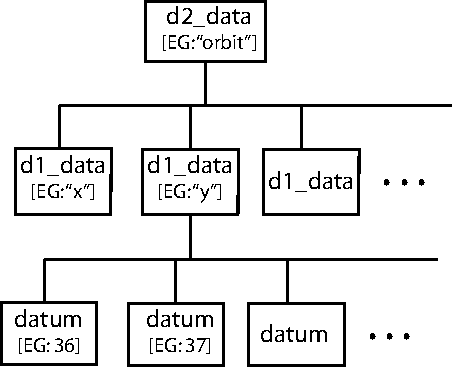
\includegraphics[width=4in]{data-tree.pdf}
  \caption[Data tree structure]
{A \vn{d2_data} structure holds a set of \vn{d1_data} structures. 
A \vn{d1_data} structure holds an array of datums.}
  \label{f:data.tree}
\end{figure}

\index{d2_data}\index{d1_data}
The horizontal orbit at a particular BPM is an example of an
individual \vn{datum}.  For ease of manipulation, arrays of datums are
grouped into what is called a \vn{d1_data} structure. Furthermore,
sets of \vn{d1_data} structures are grouped into what is called a
\vn{d2_data} structure.  This is illustrated in
Figure~\ref{f:data.tree}.  For example, a \vn{d2_data} structure for
orbit data could contain two \vn{d1_data} structures --- one
\vn{d1_data} structure for the horizontal orbit data and another
\vn{d1_data} structure for the vertical orbit data. Each datum of,
say, the horizontal orbit \vn{d1_data} structure would then correspond
to the horizontal orbit at some point in the machine.

When issuing \tao commands, all the
data associated with a \vn{d2_data} structure is specified using the
\vn{d2_data} structure's \vn{name}.  The data associated with a
\vn{d1_data} structure is specified using the format
\begin{example}
  d2_name.d1_name
\end{example}
For example, if a \vn{d2_data} structure has the
name ``\vn{orbit}'', and one of its \vn{d1_data} structures has the
name ``\vn{x}'', then \tao commands that refer to the data in this
\vn{d1_data} structure use the name ``\vn{orbit.x}''. Sometimes there
is only one \vn{d1_data} structure for a given \vn{d2_data}
structure. In this case the data can be referred to simply by using
the \vn{d2_data} structure's name. The individual datums can be
referred to using the notation
\begin{example}
  <d2_name>.<d1_name>[<list_of_datum_indexes>]
\end{example}
For example, \vn{orbit.x[10]} refers to the horizontal orbit datum
with index 10. Notice that the beginning (lowest) datum index is user
selectable and is therefore not necessarily 1. 

It is important to note that the name given to \vn{d2_data} and \vn{d1_data}
structures is arbitrary and does not have to correspond to the 
type of data contained in the 
structures. In fact, a \vn{d1_data} array can contain heterogeneous data types.
Thus, for example, it is perfectly permissible (but definitely not recommended) 
to set up the data structures so that, say, \vn{orbit.x[10]} 
is the $a$-mode emittance at a certain element and \vn{orbit.x[11]}
is the $b$-mode beta function at the same element.

Ranges of data can be referred to using using a comma \vn{,} to
separate the indexes combined with the notation \vn{n1:n2} to specify
all the datums between \vn{n1} and \vn{n2} inclusive. For example
\begin{example}
  orbit.x[3:6,23]
\end{example}
refers to datums 3, 4, 5, 6, and 23. 

If multiple universes are present, then, as explained in
\sref{s:universe}, the prefix \vn{"@"} may be used to specify which
universe the data applies to. The general notation is
\begin{example}
  [<universe_range>]@<d2_name>.<d1_name>[<datum_index>]
\end{example}
Examples:
\begin{example}
  [2:4,7]@orbit.x ! The \vn{orbit.x} data in universes 2, 3, 4 and 7.
  [2]@orbit.x     ! The \vn{orbit.x} data in universe 2. 
  2@orbit.x       ! Same as "2@orbit.x".
  orbit.x         ! The \vn{orbit.x} data in the current default universe.
  -1@orbit.x      ! Same as "orbit.x".
\end{example}

As explained in Section~\sref{s:data.anatomy}, each individual datum
has a number of components. The syntax to refer to a component is:
\begin{example}
  d2_name.d1_name[datum_index]|component
\end{example}
For example:
\begin{example}
  orbit.x[3:10]|meas     ! The measured data values
\end{example}

In referring to datums, a ``\vn{*}'' can be used as a wild card to 
denote ``all''. Thus:
\begin{example}
  *@orbit.x       ! The \vn{orbit.x} data in all universes.
  *               ! All the data in the current default universe.
  *.*             ! Same as "*"
  *@*             ! All the data in all the universes. 
  *@*.*           ! Same as "*@*"
  orbit.x[*]|meas ! All measured values of orbit.x
  orbit.x[]|meas  ! No values. That is, the empty set.
  orbit.x|meas    ! Same as orbit.x[*]|meas.
\end{example}
The last example shows that when referring to an entire block of data
encompassed by a \vn{d1_data} structure, the \vn{[*]} can be omitted.

%------------------------------------------------------------------------
\section{Anatomy of a Datum}
\label{s:data.anatomy}

Each datum has a number of components associated with it:
\begin{example}
  data_type        ! Character: Type of data: "orbit.x", etc.
  ele_name         ! Character: Name of lattice element where datum is evaluated.
  ele_start_name   ! Character: Name of starting lattice element in a range.
  ele_ref_name     ! Character: Name of reference lattice element.
  merit_type       ! Character: Type of constraint: "target", "max", etc.
  data_source      ! Character: How the datum is calculated. "lat", "beam", etc.
  ix_ele           ! Integer: Index of "ele" in the lattice element list.
  ix_branch        ! Integer: Lattice branch index.
  ix_ele_start     ! Integer: Index of "ele_start" in the lattice element list.
  ix_ele_ref       ! Integer: Index of "ele_ref" in the lattice element list.
  ix_ele_merit     ! Integer: Lattice index where merit is evaluated.
  ix_d1            ! Integer: Index number in d1_data structure
  ix_data          ! Integer: Index in the global data array
  ix_dModel        ! Integer: Row number in the dModel_dVar derivative matrix.
  ix_bunch         ! Integer: Bunch number to get the data from.
  eval_point       ! Character/integer: Evaluation point relative to the lattice element.
  meas             ! Real: Measured datum value. 
  ref              ! Real: Measured datum value from the reference data set.
  model            ! Real: Datum value as calculated from the model.
  design           ! Real: What the datum value is in the design lattice.
  old              ! Real: Used by \tao to save the model at some previous time.
  base             ! Real: The value as calculated from the base model.
  fit              ! Real: This value is not used by \tao.
  invalid          ! Real: The value used for delta_merit if good_model = False.
  delta_merit      ! Real: Diff used to calculate the merit function term 
  weight           ! Real: Weight for the merit function term
  merit            ! Real: Merit function term value: weight * delta^2
  s                ! Real: longitudinal position of ele.
  s_offset         ! Real: Offset of the evaluation point.
  exists           ! Logical: Does the datum exist?
  good_model       ! Logical: Does the model  component contain a valid value?
  good_design      ! Logical: Does the design component contain a valid value?
  good_base        ! Logical: Does the base   component contain a valid value?
  good_meas        ! Logical: Does the meas   component contain a valid value?
  good_ref         ! Logical: Does the ref    component contain a valid value?
  good_user        ! Logical: Does the user want this datum used in optimization?
  good_opt         ! Logical: Can be used in Tao extensions.
  good_plot        ! Logical: Can be used in Tao extensions.
  useit_plot       ! Logical: Is this datum to be used in plotting?
  useit_opt        ! Logical: Is this datum to be used for optimization?
\end{example}
When running \tao, the \vn{show data}
(\sref{s:show}) command can be used to view the components of a datum. 
The \vn{set} command (\sref{s:set}) can be used to set some of these components.

\begin{description}
  \item[base] \Newline
The value of the datum as calculated from the base lattice (\sref{s:datum.values}).
  \item[data_source] \Newline
The \vn{data_source} component specifies where the data is coming from
(\sref{s:data.source}).
  \item[data_type] \Newline
The type of data (\sref{s:data.types}). For example, \vn{beta.a}. At startup, if the
\vn{data_type} is not specified, it is set to \vn{<d2_name>.<d1_name>} where
\vn{<d2_name>} is the name of the associated \vn{d2} data structure and \vn{<d1_name>} is 
the name of the associated \vn{d1} data structure (\sref{s:init.data}).
  \item[delta_merit] \Newline
Difference used to calculate the contribution of the datum to the merit function (\sref{s:lattice.correction}).
  \item[design] \Newline
The value of the datum as calculated from the design lattice (\sref{s:datum.values}).
  \item[ele_name] \Newline
Name of the associated lattice element where the datum is evaluated
(\sref{s:datum.opt}). Also see \vn{eval_point} and \vn{s_offset} components.
  \item[ele_start_name] \Newline
Starting element of a range of lattice elements (\sref{s:data.lat.ele}).
  \item[ele_ref_name] \Newline
Reference lattice element (\sref{s:data.lat.ele}).
  \item[eval_point] \Newline
Used with \vn{s_offset} to determine where the datum is evaluated at (\sref{s:dat.eval}).
  \item[exists] \Newline
Set by \tao to True if the datum exists (\sref{s:datum.opt}). 
  \item[fit] \Newline
Not used by \tao. Can be used with custom code.
  \item[good_base] \Newline
Set by \tao. Is the \vn{base} value valid?
  \item[good_design] \Newline
Set by \tao. Is the \vn{design} value valid?
  \item[good_meas] \Newline
Set by \tao. Is the \vn{meas} value valid?
  \item[good_model] \Newline
Set by the user. Is the \vn{meas} value valid?
  \item[good_opt] \Newline
Set by the user. Is the datum valid for optimization?
  \item[good_plot] \Newline
Set by the user. Is the datum to be used in plotting?
  \item[good_ref] \Newline
Set by the user. Is the \vn{ref} value valid?
  \item[good_user] \Newline
Set by the user. Is the datum valid for optimization or plotting?
  \item[invalid] \Newline
The value used for \vn{delta_merit} if good_model = False. 
  \item[ix_branch] \Newline
The index of the lattice branch that contains \vn{ele}, \vn{ref_ele}, and \vn{start_ele}.
  \item[ix_ele] \Newline
Index of the lattice element where the datum is evaluated at. 
  \item[ix_ele_start] \Newline
Index of the start element.
  \item[ix_ele_ref] \Newline
Index of the reference element.
  \item[ix_ele_merit] \Newline
Set by \tao. When the \vn{merit_type} is set to \vn{max} or \vn{min} and there is a range
of elements that over which the there is an evaluation, ix_ele_merit is set to the element
where the value is the \vn{max} or \vn{min}.
  \item[ix_d1] \Newline
Index of the associated \vn{d1_data} array.
  \item[ix_data] \Newline
For convenience, all the datums of a given universe are put into one large array. \vn{ix_data} is the index
of the datum in this array. This is useful for debugging purposes.
  \item[ix_dModel] \Newline
For optimization, \tao creates a derivative matrix dMerit_i/dVar_j. \vn{ix_dmodel} is set
to the i\Th column of this matrix. This is useful for debugging purposes
  \item[ix_bunch] \Newline
For datums that have \vn{data_source} set to \vn{beam}, \vn{ix_bunch} selects which bunch
of the beam the datum is evaluated at.
  \item[meas] \Newline
The value of the datum as obtained from some measurement (\sref{s:datum.values}).
  \item[merit] \Newline
The contribution to the merit function due to this datum (\sref{s:lattice.correction}).
  \item[merit_type] \Newline
The type of merit (\sref{s:generalized.design}). 
  \item[model] \Newline
The value of the datum as calculated from the \vn{model} lattice (\sref{s:datum.values}).
  \item[old] \Newline
A datum value that was saved at some point in \tao's calculations. This value
can be ignored (\sref{s:datum.values}).
  \item[ref] \Newline
The reference datum value as obtained from some reference measurement (\sref{s:datum.values}).
  \item[s] \Newline
Longitudinal $s$-position of the lattice element.
  \item[s_offset] \Newline
Offset of the evaluation point when there is an associated lattice element (\sref{s:dat.eval}).
  \item[useit_opt] \Newline
Datum is possibly valid for optimization. \vn{useit_opt} is set by \tao using the other
\vn{logicals} components. A datum is used in the optimization if both \vn{useit_opt} and
\vn{good_meas} are true.
  \item[useit_plot] \Newline
Datum is valid for plotting
  \item[weight] \Newline
Weight used in evaluating the contribution of the datum to the merit function (\sref{s:lattice.correction}).
\end{description}

%------------------------------------------------------------------------
\section{Datum values}
\label{s:datum.values}

\index{data!measured}\index{data!reference}\index{data!model}
\index{data!base}\index{data!design}
A given datum has six values associated it:
\vspace{-2ex}
\begin{description}
  \vspace{-1ex}
  \item[meas] \Newline 
The value of the datum as obtained from some measurement. This is the
target or limit value that is used when running the optimizer. When
doing lattice design, the measured value corresponds to a constraint
value (\ref{c:opti}).
  \vspace{-1ex}
  \item[base] \Newline
The datum value as calculated from the \vn{base} lattice (\sref{s:lattice}).
  \vspace{-0.5ex}
  \item[design] \Newline
The value of the datum as calculated from the \vn{design} lattice (\sref{s:lattice}).
  \vspace{-0.5ex}
  \item[fit] \Newline
The \vn{fit} value is not used by \tao directly and is available for use by custom code.
  \vspace{-0.5ex}
  \item[model] \Newline
The value of the datum as calculated from the \vn{model} lattice (\sref{s:lattice}).
  \vspace{-0.5ex}
  \item[old] \Newline
A datum value that was saved at some point in \tao's calculations. This value
can be ignored.
  \vspace{-0.5ex}
  \item[ref] \Newline
The reference datum value as obtained from some reference measurement. For example,
a measurement before some variable is varied could be designated as
the \vn{reference}, and the datum taken after the variation could be 
designated the \vn{measured} datum.
\end{description}

%------------------------------------------------------------------------
\section{Evaluation Point of a Datum}.
\label{s:dat.eval}

When the datum is to be evaluated at a specific point in the lattice, that is, when there
is an associated lattice element, the default position for evaluating the datum is at the
downstream end of the element. This evaluation point can be shifted using the
\vn{eval_point} and/or \vn{s_offset} components. 

The \vn{eval_point} component can be set to one of:
\begin{example}
  beginning   ! entrance end of lattice element.
  center      ! Center of lattice element
  end         ! Exit end of lattice element. Default.
\end{example}
The evaluation point is shifted by \vn{s_offset} from the \vn{eval_point}.

If there is a reference point, the setting of \vn{eval_point} is used to determine where
the reference point is but the setting of \vn{s_offset} is ignored.

Due to internal logic considerations, Not all \vn{data_type}s are compatible with a finite
\vn{s_offset} or a setting of \vn{eval_point} to \vn{center}. The table of \vn{data_type}s
(\sref{t:data.types}) shows which \vn{data_type}s are compatible and which are not.

Another restriction is that specifying a range of elements for evaluation (that is,
specifying \vn{ele_start_name} \sref{s:init.data}) is not compatible with a finite
\vn{s_offset} or a setting of \vn{eval_point} to \vn{center}.

%------------------------------------------------------------------------
\section{Datums in Optimization}
\label{s:datum.opt}

When using optimization for lattice correction or lattice design
(\sref{c:opti}), Individual datums can be excluded from the process
using the \vn{veto} (\sref{s:veto}), \vn{restore} (\sref{s:restore}),
and \vn{use} (\sref{s:use}) commands. These set the \vn{good_user}
component of a datum. This, combined with the setting \vn{exists},
\vn{good_meas}, \vn{good_ref}, and \vn{good_opt}
determine the setting of \vn{useit_opt} which is the component that
determines if the datum is used in the computation of the merit
function. The settings of everything but \vn{good_user} is determined
by \tao

The \vn{exists} component is set by \tao to True if the datum exists
and False otherwise. A datum may not exist if the type of datum
requires the designation of an associated element but the
\vn{ele_name} component is blank. For example, a \vn{d1_data} array
set up to hold orbit data may use a numbering scheme that fits the
lattice so that , say, datum number 34 in the array does not
correspond to an existing BPM.

The \vn{good_model} component is set according to whether a datum
value can be computed from the \vn{model} lattice. For example, If a
circular lattice is unstable, the beta function and the closed orbit
cannot be computed. Similarly, the \vn{good_design} and \vn{good_base}
components mark whether the \vn{design} and \vn{base} values
respectively are valid.

When doing optimization, the \vn{delta_merit} component is set to the
\vn{delta} value used in computing the contribution to the merit
function (\sref{s:generalized.design}). If the datum's value cannot be
computed, that is, \vn{good_model} is False, or, if the design or base
values are being used in the merit calculation, \vn{good_base} or
\vn{good_design} is False, then the \vn{invalid} component is used for
\vn{delta_merit}.

\vn{good_meas} is set True if the \vn{meas} component value is set in
the data initialization file (\sref{s:init.data}) or is set using the
\vn{set} command (\sref{s:set}). Similarly, \vn{good_ref} is set True
if the \vn{ref} component has been set. \vn{good_ref} only affects the
setting of \vn{useit_opt} if the optimization is using reference data
as set by the global variable \vn{opt_with_ref} (\sref{s:globals}).

Finally \vn{good_opt} is meant for use in custom versions of \tao
(\sref{c:custom.tao}) and is always left True by the standard \tao code.

Example of using a \vn{show data} (\sref{s:show}) to check the logicals
in a datum:
\begin{example}
  Tao> show data 3@beta[1]

  Universe:   3
  %ele_name          = IP_L0
  %ele_ref_name      =
  %ele_start_name    =
  %data_type         = beta.a
      ... etc ...
  %exists            =  T
  %good_model        =  T
  %good_meas         =  F
  %good_ref          =  F
  %good_user         =  T
  %good_opt          =  T
  %good_plot         =  F
  %useit_plot        =  F
  %useit_opt         =  F
\end{example}
Here \vn{useit_opt} is False since \vn{good_meas} is False and
\vn{good_meas} is False since the \vn{meas} value of the datum (not
shown) was not set in the \tao initialization file.

%------------------------------------------------------------------------
\section{Data_source}
\index{data!data_source}
\label{s:data.source}

The \vn{data_source} component specifies where the data is 
coming from. Possible values are:
\begin{example}
  "beam"        ! Data from from multiparticle beam distribution
  "data"        ! Data from from a \tao datum in a data array.
  "lat"         ! Data from from the lattice.
\end{example}
If \vn{data_source} is set to \vn{"beam"}, the data is calculated
using multiparticle tracking.  If \vn{data_source} is set to
\vn{"lat"}, the data is calculated using the ``lattice'' which here
means everything {\em but} multiparticle tracking.  For example, the
\vn{"beam"} based calculation of the emittance uses the bunch sigma
matrix obtained through multiparticle tracking. The \vn{"lat"} based
calculation of the emittance uses radiation integrals.

Some data types may be restricted as to which \vn{data_source} is
possible. For example, a datum with \vn{data_type} set to
\vn{n_particle_loss} must use \vn{"beam"} for the \vn{data_source}. 
Table~\ref{t:data.types} lists which \vn{data_source} values are valid
for what data types.

%------------------------------------------------------------------------
\section{Datum Evaluation and Associated Lattice Elements}
\index{data!associated lattice elements}
\label{s:data.lat.ele}

Datums can be divided up into two classes. In one class are the datums
that are \vn{``local''}, like the beam orbit, which need to be evaluated at
either a particular point are evaluated over some finite region of the
machine. Other datums, like the emittance, are \vn{``global''} and do not
have associated evaluation points.

As mentioned, \vn{local} datums may be evaluated at a specific point
or over some evaluation region, an evaluation region is used when, for
example, the maximum or minimum value over a region is wanted. To
specify an evaluation point, an \vn{evaluation element} must be
associated with a datum. The evaluation point will be at the exit end
of this element. To specify an evaluation region, a \vn{start element}
must also be associated with a datum along with the \vn{evaluation
element}. The evaluation region is from the exit end of the \vn{start
element} to the exit end of the \vn{evaluation element}.

In addition to the \vn{evaluation element} and the \vn{start element},
a \vn{local} datum may have an associated \vn{reference element}.  A
\vn{reference element} is used as a fiducial point and the datum value
is calculated relative to that point. For example, a datum value may
be the position of the \vn{evaluation element} relative to the
position of the \vn{reference element}. The evaluation point of a
\vn{reference element} is the exit end of that element.

The components in a datum corresponding to the \vn{evaluation
element}, the \vn{reference element}, and the \vn{start element}.  are
shown in Table~\ref{t:datum.elements}.  These three elements may be
specified for a datum by either setting the name component or the
index component of the datum. Using the element index over the element
name is necessary when more than one element in the lattice has the
same name.

\begin{table}[htb]
\centering
\begin{tabular}{lll}
  \toprule
  &\multicolumn{2}{c}{\it Data Component} \\ \cmidrule{2-3}
  {\it Element} & {\it name} & {\it index} \\ \midrule
  Reference Element  & \vn{ele_ref_name}   & \vn{ix_ele_ref}   \\
  Start Element      & \vn{ele_start_name} & \vn{ix_ele_start} \\
  Evaluation Element & \vn{ele_name}       & \vn{ix_ele}       \\ \bottomrule
\end{tabular}
\caption[The three lattice elements associated with a datum.]
{The three lattice elements associated with a datum may be
specified in the datum by setting the appropriate name component or by 
setting the appropriate index component.}
\label{t:datum.elements}
\end{table}

If a datum has an associated \vn{evaluation} element, but no
associated \vn{start} or \vn{reference} elements, the \vn{model} value
of that datum is the value of the \vn{data_type} at the \vn{evaluation}
element. For example, if a datum has:
\begin{example}
  data_type      = "orbit.x"
  ele_name       = "q12"
\end{example}
here the \vn{model} value of this datum will be the horizontal orbit
at the element with name \vn{q12}.

If a datum has an associated \vn{start} element, specified by either
setting the \vn{ele_start_name} or \vn{ix_ele_start} datum components, the
datum is evaluated over a region from the exit end of the \vn{start} element
to the exit end of \vn{evaluation} element. For example, if a datum has:
\begin{example}
  data_type      = "beta.a"
  ele_name       = "q12"
  ele_start_name = "q45"
  merit_type     = "max"
\end{example}
then the \vn{model} value of this datum will be the maximum value of
the a-mode beta function in the region from the exit end of the
element with name \vn{q12} to the exit end of the element with name
\vn{q45}. Notice that when a range of elements is used, a
\vn{merit_type} of \vn{target} does not make sense. 

Typically, in evaluating a datum over some region to find the maximum
or minimum, \tao will only evaluate the datum at the ends of the
elements with the assumption that this is good enough. If this is not
good enough, marker elements can be inserted into the lattice at
locations that matter. For example, the maximum or minimum of the beta
function typically occurs near the middle of a quadrupole so inserting
marker elements in the middle of quadrupoles will improve the accuracy
of finding the extremum beta.

If a datum has an associated \vn{reference} element, specified by either
setting the \vn{ele_ref_name} or \vn{ix_ele_ref} datum components, the
\vn{model} value of the datum is the value at the \vn{evaluation} element (or the value
over the range \vn{ele_start} to the \vn{evaluation} element if \vn{ele_start} is
specified), minus the \vn{model} value at \vn{ele_ref}. For example,
if a datum has:
\begin{example}
  data_type      = "beta.a"
  ele_name       = "q12"
  ele_start_name = "q45"
  ele_ref_name   = "q1"
  merit_type     = "max"
\end{example}
then the \vn{model} value of the datum will be the same as the
previous example minus the value of the a-mode beta function at the
exit end of element \vn{q1}. There are a number of exceptions to the
above rule and datum types treat the \vn{reference} element in a different
manner. For example, the \vn{r.} data type uses the \vn{reference} element
as the starting point in constructing a transfer matrix.

%------------------------------------------------------------------------
\section{Tao Data Types}\index{data!data Types}
\label{s:data.types}

The \vn{data_type} component of datum specifies what type of data the
datum represents. For example, a datum with a \vn{data_type} of
\vn{orbit.x} represents the horizontal orbit. Table~\ref{t:data.types} lists
what data types \tao knows about.

It is important to note the difference between the \vn{d2.d1} name
that is used to refer to a datum and the actual type of data, given by
\vn{data_type}, of the datum. The \vn{d2.d1} name is arbitrary and is
specified in the \tao initialization file (\sref{s:init.data}). Often,
these names do reflect the actual type of data. However, there is no
mandated relationship between the two. For example, it is perfectly
possible to set create a data set with a \vn{d2.d1} name of
\vn{orbit.x} to hold, say, global floor position data. In fact, the
datums in a given \vn{d1} array do not all have to be of the same
type. Thus the user is free to group data as s/he sees fit.

Description of the data types:

  \begin{description}

  \item[alpha.a, .b] \Newline
Twiss function \vn{alpha}.
  \item[apparent_emit.x, .y] \Newline
The apparent emittance is the emittance that one would calculate based
upon a measurement of the beam size\cite{b:emit}. It can be useful to
compare this to the true normal mode emittance. Also See the
\vn{norm_apparent_emit}, \vn{emit.} and \vn{norm_emit.} data types.
With \vn{data_source} set to \vn{"beam"}, \vn{apparent_emit.x} is
\begin{equation}
  \text{emit}_x = \frac{\sigma_{xx} - \eta_x^2 \, \sigma_{p_zp_z}}{\beta_a}
\end{equation}
with a similar equation for \vn{apparent_emit.y}. Here $\sigma$ is the beam size matrix
\begin{equation}
  \sigma_{r_1r_2} \equiv \left< r_1 \, r_2 \right>
\end{equation}
With \vn{data_source} set to \vn{"lat"}, The apparent emittance is
calculated from the true normal mode emittance and the Twiss
parameters (Cf.~ Eqs (4) and (5) of \cite{b:emit}).

  \item[beta.a, .b, .c] \Newline
Lattice normal mode betas.

  \item[beta.x, .y, .z] \Newline
Beam projected beta functions. \vn{beta.x} is defined by
\begin{equation}
  \beta.x = \frac{<x^{2}>}{\sqrt{<x^{2}> <x'^{2}> - <x x'>^{2}}}.
\end{equation}
with similar equations for the other planes.
The average \vn{<>} is over all the particles in the beam.

Note: If the beta function is calculated from the beam distribution,
the initial beam emittance must be set to something non-zero.

  \item[bpm_cbar.22a, .12a, .11b, .12b] \Newline
The normalized Cbar coupling parameters. The computed \vn{model} values include
detector misalignments, rotations, gain errors, etc. This type of datum is useful for
simulating how well actual coupling corrections are. See the \bmad manual for more
details.

  \item[bpm_eta.x, y] \Newline
The horizontal and vertical dispersion components. The computed \vn{model} values include
detector misalignments, rotations, gain errors, etc. This type of datum is useful for
simulating how well actual dispersion corrections are. See the \bmad manual for more
details.

  \item[bpm_orbit.x, y] \Newline
Beam Orbit. The computed \vn{model} values include detector misalignments, rotations, gain
errors, etc. This type of datum is useful for simulating how well actual orbit corrections
are. See the \bmad manual for more details.

  \item[bpm_phase.a, b] \Newline
Betatron phase. The computed \vn{model} values include detector misalignments, rotations, gain
errors, etc. This type of datum is useful for simulating how well actual orbit corrections
are. See the \bmad manual for more details.

  \item[bpm_k.22a, .12a, .11b, .12b] \Newline
Measured beam coupling components. The computed \vn{model} values include detector misalignments, rotations, gain
errors, etc. This type of datum is useful for simulating how well actual coupling corrections
are. See the \bmad manual for more details.

  \item[bunch_max, bunch_min.x, .px, .y, .py, .z, .pz] \Newline
Maximum or minimum phase space coordinate in a bunch, relative to its centroid.

  \item[c_mat.11, .12, .21, .22] \Newline
Coupling matrix components. The 2x2 C matrix describe the $x$-$y$ coupling of the beam.
See the \bmad manual for more details.

  \item[cbar.11, .12, .21, .22] \Newline
Normalized coupling matrix components. The 2x2 C matrix describe the $x$-$y$ coupling of the beam.
The normalized matrix is normalized by factors of $\beta$. See the \bmad manual for more details.

  \item[chrom.a, .b] \Newline
Chromaticities. Old names: \vn{chrom.dtune.a} and \vn{chrom.dtune.b}

  \item[chrom.dbeta.a, .dbeta.b] \Newline
The normalized change of the beta function with energy
$(1/\beta_{a,b})\partial\beta_{a,b}/\partial\delta$. Unlike the standard chromaticities,\vn{chrom.a} and \vn{chrom.b},
the these chromaticities are evaluated at individual elements.

  \item[chrom.deta.a, .deta.b] \Newline
The chromatic dispersion $\partial\eta_{x,y}/\partial\delta$. Unlike the standard
chromaticities,\vn{chrom.a} and \vn{chrom.b}, the these chromaticities are evaluated at
individual elements.

  \item[chrom.detap.a, .detap.b] \Newline
The chromatic dispersion derivatives $\partial\eta'_{x,y}/\partial\delta$. Unlike the standard
chromaticities,\vn{chrom.a} and \vn{chrom.b}, the these chromaticities are evaluated at
individual elements.

  \item[chrom.dphi.a, .dphi.b] \Newline
The chromatic betatron phase $\partial\phi_{a,b}/\partial\delta$. Unlike the standard
chromaticities,\vn{chrom.a} and \vn{chrom.b}, the these chromaticities are evaluated at
individual elements.

  \item[damp.j_a, .j_b, .j_z] \Newline
Damping partition numbers.

  \item[dpx_dx, dpy_dy, etc.] \Newline
Bunch sigma matrix ratios, <x px> / <$x^2$> \& Etc.

  \item[e_tot_ref] \Newline
The reference energy of the lattice. This is the same as the \vn{E_tot} attribute of a lattice element.
For the actual particle energy, use \vn{orbit.e_tot}.

  \item[element_attrib.<attrib_name>] \Newline
The \vn{element_attrib.<attrib_name>} data type is associated with the
lattice element attribute named \vn{<attrib_name>}. See the \bmad
(\cite{b:bmad}) manual for information on attribute names. For
example, to plot the dipole bend strength \vn{g}, the following
plot template (\sref{s:init.plot}) can be used:
\begin{example}
  &tao_template_plot
    plot%name = 'bend_g'
    plot%n_graph = 1
    plot%x_axis_type = 'index'
  /

  &tao_template_graph
    graph%name = 'g'
    graph%type = 'data'
    graph_index = 1
    graph%y%label = 'g'
    graph%n_curve = 1
    curve(1)%name = 'g'
    curve(1)%data_type = 'element_attrib.g'
    curve(1)%draw_line = F
  /
\end{example}

  \item[emit.a, .b, .c] \Newline
True normal mode (eigen) emittances.  With \vn{data_source} set to \vn{"beam"}, the
emittance is calculated from the beam sigma matrix. With \vn{data_source} set to
\vn{"lat"}, the normal mode emittance is calculated using the standard radiation
integrals.

  \item[emit.x, .y, .z] \Newline
``Projected'' emittances\cite{b:emit}. 
For a linear lattice, the emittance varies along the length
of the line while for a circular lattice there is a single emittance
number. 

With \vn{data_source} set to \vn{"beam"}, the emittance is calculated from the beam sigma
matrix. The formula for $\epsilon_x$ is
\begin{equation}
  \epsilon_x = \sqrt{ \wt\sigma_{xx} \, \wt\sigma_{p_xp_x} - \wt\sigma_{xp_x}^2}
\end{equation}
With a similar equation for $\epsilon_y$. Here $\wt\sigma$ is the energy normalized
beam size:
\begin{equation}
  \wt\sigma_{xx} = \langle x \, x \rangle - 
  \frac{\langle x \, p_z \rangle \, \langle x \, p_z \rangle}{\langle p_z \, p_z \rangle}
\end{equation}
with similar definitions for the other $\wt\sigma$ components. 
Note that the projected emittance is sometimes defined using
$x'$ and $y'$ in place of $p_x$ and $p_y$. However, in the vast
majority of cases, this does not appreciably affect the numeric
results.

See also the \vn{norm_emit.}, \vn{apparent_emit.}, and
\vn{norm_apparent_emit.} data types.

  \item[expression: <arithmetic_expression>] \Newline
\vn{<arithmetic_expression>} is an arithmetic expression (\sref{s:arithmetic.exp}) which
is evaluated to get the value of the datum. For example:
\begin{example}
  datum(i)%data_type = "expression: 1@ele::q10w[beta_a] - 2@ele::q10w[beta_a]"
\end{example}
With this, the value of the datum will be the difference between the a-mode beta at
element \vn{q10w} for universe 1 and universe 2. In this example, the source of both terms
in the expression is explicitly given as \vn{ele}.  This is not necessary if the
\vn{datum%data_source} is set to \vn{ele}
\begin{example}
  datum(i)%data_type = "expression: 1@q10w[beta_a] - 2@q10w[beta_a]"
  datum(i)%data_source = "ele"
\end{example}
An expression can also be used as the \vn{default_data_type}. In this case, the evaluation
point is implicit. For example:
\begin{example}
  default_data_source = "data"
  default_data_type = "expression: 1@beta.a - 2@beta.a"
\end{example}
which is equivalent to:
\begin{example}
  default_data_type = "expression: 1@data::beta.a - 2@data::beta.a"
\end{example}

To be valid, if an expression has a term with a \vn{data} source, the
expression must be evaluated after the \vn{data} source components are
evaluated. Data evaluation is done universe by universe starting with
universe 1, then universe 2, etc. Within a given universe, the order
of evaluation can be complicated but in this case a datum using an
expression will always be evaluated after any datum that appears
earlier in the initialization file.  In the last example above, the
expression terms involve an evaluation of \vn{beta.a} in universe 2.  
Therefore, this expression datum should
be in universe 2 or higher. Notice that while all datums must be
assigned a universe, in this case, since all the terms explicitly give
a universe number, the value of the datum will be independent of the
universe it is in.

In the above examples, the lattice elements involved were explicitly specified.
To apply an expression to the lattice element associated with a datum use
the syntax ``\vn{ele::\#}'' to represent the associated lattice element. Example:
\begin{example}
  default_data_type = "expression: ele::#[k1] * ele::#[l]"
  datum(1:4)%ele_name = "Q01", "Q02", "Q03", "Q04"
\end{example}
In this example the values of the four datums will the integrated quadrupole strength K1*L
of the associated lattice elements \vn{Q01} for the first datum, etc.

  \item[floor.x, .y, .z] \Newline
Position of the element in the global ``floor'' coordinate system. This is the nominal
position ignoring any misalignments. See the \bmad manual for details on the global
coordinate system. See also \vn{rel_floor.} and \vn{will.}.

  \item[floor.theta, .phi, .psi] \Newline
Orientation of the element in the global ``floor'' coordinate system. This is the nominal
position ignoring any misalignments. See the \bmad manual for details on the global
coordinate system. See also \vn{rel_floor.}.

  \item[gamma.a, .b] \Newline
Normal mode Twiss gamma function.

  \item[k.11b, .12a, .12b, .22a] \Newline
Measured beam coupling parameters. See also \vn{bpm_k.11b, ...}.

  \item[momentum] \Newline
Particle momentum.

  \item[momentum_compaction] \Newline
Momentum compaction factor. Also see \vn{r56_compaction}.

  \item[multi_turn_orbit.x, .y, .z, .px, .py, .pz] \Newline
Used for storing the orbit over many turns. Only used for plotting purposes.
See \sref{s:plot.data} for more details.

  \item[n_particle_loss] \Newline
If the reference element is not specified, \vn{n_particle_loss} gives
the number of particles lost at the evaluation element. If the
reference element is specified, \vn{n_particle_loss} gives the
cumulative loss between the exit end of the reference element and the
exit end of the evaluation element. That is, this sum does not count
any losses at the reference element itself. If neither reference nor
evaluation element is given then the total number of lost particles is
given.

  \item[norm_apparent_emit.x, .y] \Newline
Energy normalized apparent emittance. The normalization is the standard gamma factor:
\Begineq
  \text{emit}_{\text{norm}} = \gamma \, \text{emit}
\Endeq
See the \vn{apparent_emit.x, .y} data type for more details.

  \item[norm_emit.a, .b, .c] \Newline
Energy normalized normal mode emittance. The normalization is the standard gamma factor:
\Begineq
  \epsilon_{norm} = \gamma \, \epsilon
\Endeq

  \item[norm_emit.x, .y, .z] \Newline
Energy normalized projected emittance. The normalization is the standard gamma factor:
\Begineq
  \epsilon_{norm} = \gamma \, \epsilon
\Endeq

  \item[normal.<type>.$i$.<monomial>] \Newline
Components of the normal form decomposition of the one-turn-map $M$ for a ring. 
Possible settings for \vn{type} is
\begin{example}
  M, A, A_inv, dhdj, ReF, or ImF
\end{example}      
$i$ is an integer between 1 and 6, and \vn{monomial} is a six digit number that specifies
a monomial. For example: \vn{100001}. 

In the symplectic case:
\Begineq \label{normalform1}
  M = A\circ \exp\left(:h:\right)\circ A^{-1},
\Endeq
where $A$ is the nonlinear normalizing map, and $h$ is a function of the amplitudes $J_i =
(1/2)(x_i^2 + p_i^2)$ only. The amplitude dependent tune shifts are given by $\mu_i =
-dh/dJ_i$, and can be accessed through \vn{normal.dhdj}. Terms of $A$ and $A^{-1}$ can be
accessed through \vn{normal.A} and \vn{normal.A_inv}.  In the general case,
\Begineq \label{normalform2}
M = A_1\circ C \circ L \circ \exp\left(F\cdot\nabla\right)I\circ C^{-1} \circ A_1^{-1}.
\Endeq
Here $C$ is the linear map to the resonance basis: $h_\pm = x \pm i p$, $L$ is a complex
linear map, $A_1$ is the (real) first order normalizing map, and $I$ is the identity
map. All of the nonlinearities are therefore in the complex vector field $F$. The real and
imaginary parts of $L$ and $F$ can be accessed through \vn{normal.ReF}, \vn{normal.ImF},
\vn{normal.ReL}, and \vn{normal.ImL}.

  \item[null] \Newline
A \vn{null} data type is used for data where \tao is not able to calculate a model value. Such data
cannot be used in an optimization. For example, in a linac where the beam intensity is measured at
the BPMs, \tao has no model for calculating the current variation down the linac. Nevertheless, it
could be useful to read in the measured values and plot them.

  \item[orbit.amp_a, .amp_b] \Newline
``Invariant'' amplitude of the orbital motion.

  \item[orbit.norm_amp_a, .norm_amp_b] Newline
Energy normalized ``invariant'' amplitude of the orbital motion.

  \item[orbit.e_tot] \Newline
The \vn{orbit.e_tot} data type gives the total energy of a tracked particle (with
\vn{data_source} = \vn{lat}) or the average energy of a beam (with \vn{data_source} =
\vn{beam}).

Notice that this is different from the \vn{E_tot} attribute of a lattice element which
is the reference energy at that element.

  \item[orbit.x, .y, .z, .px, .py, .pz] \Newline
Orbit position and momenta

  \item[periodic.tt.$ijklm\ldots$] \Newline
This is like the \vn{tt.} datum except here the terms are from the
periodic Taylor map defined by
\Begineq
  T_p \equiv (T_0 - I_4)^{-1}
\Endeq
Here $T_p$ is the
periodic map, $T_0$ is the one-turn map from some point back to that
point, and $I_4$ is a linear map defined by the matrix
\Begineq
  I_4 \equiv 
    \begin{pmatrix}
      1 &   &   &   &   &   \\
        & 1 &   &   &   &   \\
        &   & 1 &   &   &   \\
        &   &   & 1 &   &   \\
        &   &   &   & 0 &   \\
        &   &   &   &   & 0
    \end{pmatrix}
\Endeq
The periodic map give information about the closed orbit, dispersion,
etc. For example, the zeroth order terms are the closed orbit, the r16
term gives the horizontal dispersion, etc.

If a reference lattice element is specified, the map $T_0$ will be
the transfer map from the reference element to the evaluation element.

Note: If the reference element is not specified, or if the reference
element is the same as the evaluation element, this data type cannot
be used with a linear lattice.

  \item[phase.a, .b] \Newline
Betatron phase.  If a \vn{d1_data} array has a set of
\vn{phase} datums, and if the reference element is {\em not}
specified, the average phase used for optimizations ($D$ in
\Eq{m1}) and plotting for all the datums within a \vn{d1_data}
array are set to zero by adding a fixed constant to all the datums.
This is done since, without a reference point that defines a zero
phase, the overall average phase is arbitrary and so the average phase
is taken in \tao to be zero. This can be helpful in optimizations
since one does not have to worry about arbitrary offsets between the
\vn{model} and \vn{measured} values. If the reference element is
specified then there is no arbitrary constant in the evaluation.

  \item[phase_frac.a, .b] \Newline
Fractional betatron phase. Also see the discussion under \vn{phase.a, .b}.

  \item[phase_frac_diff] \Newline
Fractional betatron phase difference between the $a$ and $b$ normal modes. 
$-\pi < d\phi_{\mbox{frac}} < \pi$

  \item[photon.intensity] \Newline
Photon total intensity.

  \item[photon.intensity_x, .intensity_y] \Newline
Photon intensity components in the horizontal and vertical planes.

  \item[photon.phase_x, .phase_y] \Newline
Photon phases in the horizontal and vertical planes.

  \item[ping_a.amp_x, .phase_x, .amp_y, .phase_y, .cos_y, .sin_y] \Newline
Phase and amplitude response at a BPM from turn-by-turn data acquired after the beam is
pinged. Ignoring damping, the beam response will be the sum of three components, one for
each beam oscillation eigenmode. \vn{ping_a} data is for the response at the \vn{a}-mode
frequency. 

At each BPM, the response will have a component in the \vn{x} (horizontal) and \vn{y}
(vertical) planes. If there is no coupling, vertical response for the \vn{a}-mode
component is zero. The \vn{a}-mode response can be characterized by the equation
\begin{align}
  x_a(n) &= A_{ax} \, \sin(n \, \omega_a + \phi_{ax} + \phi_{a0}) \CRNO
  y_a(n) &= A_{ay} \, \sin(n \, \omega_a + \phi_{ay} + \phi_{a0})
\end{align}
where $\omega_a$ is the $a$-mode tune, $x_a(n)$ and $y_a(n)$ are the horizontal and
vertical positions of the \vn{a}-mode component on the n\Th turn. $A_{ax}$ and $A_{ay}$
are the response amplitudes, $f_a$ is the \vn{a}-mode frequency $\phi_{ax}$ and
$\phi_{ay}$ are the oscillation phases, and $\phi_{a0}$ is an overall phase dependent upon
how turn $n = 0$ is defined. 
In terms of \tao's data parameters, the correspondence is
\begin{example}
    ping_a.amp_x   \(\longrightarrow A_{ax}\)
    ping_a.phase_x \(\longrightarrow \phi_{ax}\)
    ping_a.amp_y   \(\longrightarrow A_{ay}\)
    ping_a.phase_y \(\longrightarrow \phi_{ay}\)
    ping_a.sin_y   \(\longrightarrow A_{ay} \, \sin \phi_{ay}\)
    ping_a.cos_y   \(\longrightarrow A_{ay} \, \cos \phi_{ay}\)
\end{example}
In terms of how \tao analyses ping data, only differences in phases are important so $\phi_{a0}$ is
ignorable. 

The response can be related to the lattice Twiss parameters as given by Eq.~(7) of reference
\cite{b:beta.meas}
\begin{align}
  x_a(n) &=  A_a \, \sqrt{\beta_a} \, \cos(n \omega_a) , \CRNO
  y_a(n) &= -A_a \, \sqrt{\beta_b} \Bigl( \cbar{22} \, \cos(n \omega_a) +
     \cbar{12} \, \sin(n \omega_a) \Bigr)
  \label{xabno}
\end{align}

Roughly, if the coupling is not large, the ``in-plane'' \vn{x} oscillation is insensitive to any
coupling so that \vn{ping_a.amp_x} and \vn{ping_a.phase_x} can be directly related to the Twiss
parameters computed without coupling. On the other hand, the ``out-of-plane'' \vn{y} oscillation is
a direct measure of the coupling. This can be used to measure and correct skew-quadrupole
errors. Since the design coupling in many machines is zero or very small, in such cases the
\vn{ping_a.sin_y} and \vn{ping_a.cos_y} datums are better for analysis as opposed to the
\vn{ping_a.amp_y} and \vn{ping_a.phase_y} datums since the value of \vn{ping_a.phase_y} is
meaningless when the local coupling, and hence \vn{ping_a.amp_y}, is zero.

For the \vn{design} and \vn{model} values of a datum, \Eq{xabno} is used with $A_a$ taken
to be unity. To be able to compare the \vn{design} and/or \vn{model} values with the
actual data stored in \vn{meas} and/or \vn{ref}, the \vn{meas} values will be multiplied by a
constant $C_m$ computed so that the average \vn{meas} value is equal to the average
\vn{model} value:
\Begineq
  C_m \, \sum \text{ping_a.amp_x}_\text{meas} = \sum \text{ping_a.amp_x}_\text{model}
\Endeq
where the sums are over all \vn{ping_a.amp_x} data points where the \vn{exists},
\vn{good_model}, \vn{good_user}, and \vn{good_meas} components (\sref{s:data.anatomy}) are
all true. The \vn{ping_a.amp_y} data points are not used for the computation of $C_m$
since, with a decoupled lattice, the \vn{model} values are zero.

There is a similar multiplier defined for the reference data. The values of these two
multipliers are shown with the \vn{show data} command.

  \item[ping_b.amp_y, .phase_y, .amp_x, .phase_x, .sin_x, .cos_x] \Newline
Similar to \vn{ping_a} except this is for the \vn{b}-mode component of the response.  Here
the \vn{design} and \vn{model} values are calculated from Eq.~(8) of reference
\cite{b:beta.meas}:
\begin{align}
  x_b(n) &= A_b \, \sqrt{\beta_a} \Bigl( \cbar{11} \, \cos(n \omega_b) -
     \cbar{12} \, \sin(n \omega_b) \Bigr) , \CRNO
  y_b(n) &= A_b \, \sqrt{\beta_b} \, \cos(n \omega_b) .
  \label{yabno}
\end{align}
with \vn{A_b} taken to be unity for the evaluation.

The corresponding multiplicative values are derived from \vn{ping_b.amp_y} in an analogous
fashion to the multiplicative values for the $a$-mode ping data.

  \item[r.$ij$] \Newline
Terms of the linear transfer map. $1 \le i,j \le 6$.

  \item[ \begin{tabular}{@{}l}
  rad_int.i1, .i2, .i2_e4, .i3, .i3_e7, .i4a, .i4b, .i4z, .i5a, .i5b, .i5a_e6, .i5b_e6 \\
  rad_int1.i1, .i2, .i2_e4, .i3, .i3_e7, .i4a, .i4b, .i4z, .i5a, .i5b, .i5a_e6, .i5b_e6
  \end{tabular}] \Newline
Synchrotron radiation integrals. See the \bmad manual for details.
The \vn{rad_int1.xxx} datums are the radiation integrals over a single element.
With the \vn{rad_int.xxx} datums, the integral is from \vn{ele_ref} to \vn{ele}.
\begin{example}
  .i1         ! I1 radiation integral
  .i2         ! I2 radiation integral
  .i2_e4      ! Energy normalized I2 radiation integral
  .i3         ! I3 radiation integral
  .i3_e7      ! I3 radiation integral
  .i4a        ! $a$ mode I4 radiation integral
  .i4b        ! $b$ mode I4 radiation integral
  .i4z        ! Sum of I4a, and I4b radiation integrals
  .i5a        ! $a$ mode I5 radiation integral
  .i5b        ! $b$ mode I5 radiation integral
  .i5a_e6     ! Energy normalized I5a
  .i5b_e6     ! Energy normalized I5b
\end{example}

  \item[r56_compaction] \Newline
This datum is defined to be
\Begineq
  M_{5,6} + \sum_{i=1}^4 M_{5,i} \, \eta_i
\Endeq
where $\Bf M$ is the transfer matrix between the reference element and the element where the datum
is evaluated and $\eta$ is the dispersion vector evaluated at the reference element.

This datum is closely related to the momentum compaction. When \vn{r56_compaction} is evaluated
from the start of the lattice to the end, the value of \vn{r56_compaction} will be related to the
momentum compaction via:
\begin{example}
  r56_compaction = -momentum_compaction * L
\end{example}
where \vn{L} is the length of the lattice. 

  \item[ref_time] \Newline
This is the time the reference particle passes the exit end of the element.
If the particle is ultra-relativistic then this is just $c * s$ where $s$
is the longitudinal distance from the start of the lattice.

  \item[rel_floor.x, .y, .z, .theta] \Newline
This is the global floor position at the exit end of the evaluation
element relative to the exit end of the reference element in a global
coordinate system where the exit end of the reference element is taken to be at
\vn{x = y = z = theta = phi = 0}. See the \bmad manual for details on
the global coordinate system. See also \vn{floor.} and \vn{wall.}.

  \item[sigma.x, .y, .z, .px, .py, .pz, .$ij$, .Lxy] \Newline
Beam sizes \vn{sigma.x}, \vn{sigma.px}, etc., and angular momentum
\vn{sigma.Lxy} = $<xp_x - yp_x>$ are calculated from the beam sigma matrix
if the \vn{data_source} is set to \vn{beam} and calculated from the linear
Twiss parameters if the \vn{data_source} is set to \vn{lat}.

\vn{sigma.$ij$} with $1 \le i,j,k,\ldots \le 6$ are components of the beam sigma matrix.

Irregardless of the setting of \vn{data_source}, the beam emittance and longitudinal sigma
values will be taken from the \vn{beam_init} structure (\sref{s:beam.init}) and {\em not}
any emittances or longitudinal sigma values specified in the lattice file.

  \item[t.$ijk$,  tt.$ijklm\ldots$] \Newline
Taylor map components between two points with $1 \le i,j,k,\ldots \le 6$.  The difference
between \vn{t.$ijk$} and \vn{tt.$ijklm\ldots$} is that \vn{t.$ijk$} is restricted to
exactly three indices and \vn{tt.$ijklm\ldots$} is not. \vn{t.$ijk$} is superfluous but is
keep for backwards compatibility.

Calculation of \vn{t.$ijk$} and \vn{tt.$ijklm\ldots$} datums involve symplectic
integration through lattice elements. One point to be kept in mind is that results will be
dependent upon the integration step size through an element set by the \vn{ds_step}
attribute of that element (see the \bmad manual for more details). When a smooth curve
(\sref{s:template}) is plotted for \vn{t.$ijk$} and \vn{tt.$ijklm\ldots$} data types, and
the longitudinal (\vn{"s"}) position is used for the x-axis, the integration step used in
generating the points that define this curve will be decreased if the s-distance between
points is smaller than the \vn{ds_step}.  In this case, discrepancies between the plot and
datum values may be observed.

  \item[time] \Newline
Time (in seconds) a particle or the bunch centroid is at the evaluation element.

  \item[tune.a, .b] \Newline
Tune in radians.

  \item[unstable.orbit] \Newline
The \vn{unstable.orbit} datum is used for linear lattices in an
optimization to avoid unstable solutions (\sref{s:generalized.design}).

For single particle tracking, the value of an \vn{unstable.orbit}
datum is zero if the tracked particle survives (has not been lost) up
to the evaluation element and, if it has been lost, is set to
\Begineq
 1 + i_{\mbox{ele}} - i_{\mbox{lost}} + \frac{1}{2}
 \left[ \tanh\left( \frac{r_{orbit}}{r_{lim}} - 1 \right) - E \right]
\Endeq
where $i_{\mbox{ele}}$ is the index of the evaluation element in the
lattice and $i_{\mbox{lost}}$ is the index of the element where the
particle was lost. In the above equation, $E$ is the function
\Begineq
  E = 
  \begin{cases}
    1 & \text{if the particle is lost at the exit end of the element.} \\
    0 & \text{if the particle is lost at the entrance end of the element.}
  \end{cases}
\Endeq
In the abouve equation, $r_{orbit}$ is the particle amplitude at the
point of loss and $r_{lim}$ is the aperture limit. The form of the
above equation has been choisen so that the datum value will be
monotonic with increasing stability.

The default for the evaluation element, if \vn{ele_name} nor
\vn{ix_ele} is not specified, is to use the last element in the
lattice. 

When tracking beams, the value of \vn{unstable.orbit} is the averaged
value over all particles in the bunch.

  \item[unstable.ring] \Newline
\vn{unstable.ring} is used for storage rings. The value of an
\vn{unstable.ring} datum is zero if the ring is stable and set to the
largest growth rate of all the normal modes of oscillation if the ring
is unstable. \vn{unstable.ring} is used in an optimization to avoid
unstable solutions (\sref{s:generalized.design}).

\begin{figure}
  \centering
  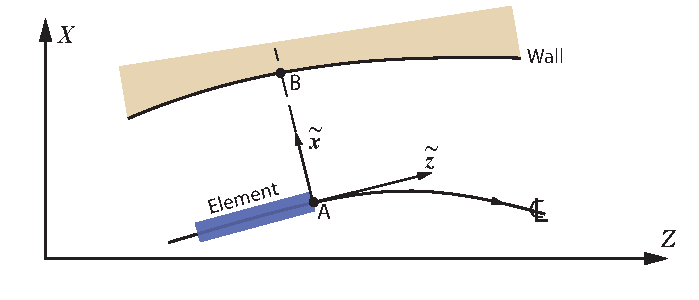
\includegraphics[width=5in]{building-wall-constraint.pdf}
  \caption[Building wall datum]
{A \vn{wall.} datum is a measure of the distance between the
centerline of a machine and the walls of the containment building.}
  \label{f:wall.constraint}
\end{figure}

  \item[wall.left_side, .right_side] \Newline
The \vn{wall} data data type is used to constrain the shape of a machine to fit
inside a building's walls (\sref{s:building.wall}). The general layout is shown in
Figure~\ref{f:wall.constraint}. The machine centerline is projected onto the horizontal
$(Z, X)$ plane in the Global (floor) coordinate system. Point \vn{A} is an evaluation
point at the exit end of some element. $\wt z$ is the projection of the local $z$-axis
onto the $(Z, X)$ plane and $\wt x$ is the coordinate in the $(Z, X)$ plane perpendicular
to $\wt z$. In the typical situation, where a machine is planer (no out-of-plane bends),
the $\wt z$-axis corresponds to the local $z$-axis and the $\wt x$-axis corresponds to the
$x$-axis (see the \bmad manual for an explanation of local and global coordinate systems).

The distance from the machine at point \vn{A} to the wall is defined to be the distance
from \vn{A} to a point \vn{B} on the wall where point \vn{B} is along the $\wt x$ axis
(has $\wt z = 0$) as shown in Figure~\ref{f:wall.constraint}.

By definition, the \vn{``left side''} of the machine corresponds to be the $+\wt x$ side
and the \vn{``right side''} corresponds to be the $-\wt x$ side. That is, left and right
are relative to someone looking in the same direction as the beam is
propagating. Correspondingly, there are two wall data types: \vn{wall.left_side} and
\vn{wall.right_side}. With the \vn{wall.left_side} data type, the datum value is positive
if point \vn{B} is on the left side and negative if on the right. Vice versa for a
\vn{wall.right_side} datum.  If there are multiple wall points \vn{B}, that is, if there
are multiple points on the wall with $\wt z = 0$, the datum value will be the minimum
value. Notice that only wall sections that have a \vn{constraint} matching the datum will
be used when searching for possible points \vn{B}. If there are no wall points with $\wt z
= 0$, the datum value is set to a large number.

For \vn{wall} data there can be no reference element since this does
not make sense.

  \item[wire.<angle>] \Newline
\vn{wire} data simulates the measurement of a wire scanner. The angle
specified is the angle of the wire with respect to the horizontal
axis. The measurement then measures the second moment $<uu>$ along an
axis which is 90 degrees off of the wire axis. For example,
\vn{wire.90} is a wire scanner oriented in the vertical direction and
measures the second moment of the beam along the horizontal axis,
$<xx>$. The resultant data is not the beam size, but the beam size
squared.

  \end{description}


\index{data!calculation method}
\index{unstable.orbit}\index{beta}\index{alpha}\index{eta}\index{eta}
\index{etap}\index{phase}\index{orbit}\index{wire}\index{building wall}\index{spin}
\index{cbar}\index{coupling}\index{floor}\index{r}\index{t}\index{tt}
\index{rad_int.i5a_e6}\index{rad_int.i5b_e6}\index{s_position}\index{e_tot}
\index{unstable.ring}\index{emittance}\index{chrom}\index{norm_emittance}
\index{sigma}\index{dpx_dx}\index{dpy_dy}\index{dpz_dz}\index{dpa_da}
\index{dpb_db}\index{rad_int.i1}\index{rad_int.i2}\index{rad_int.i2_e4}
\index{rad_int.i3}\index{rad_int.i3_e7}

%----------------------------------------------------------------------------------------------

{\tt\small
\begin{longtable}{llll} 
  \caption{Predefined Data Types in Tao}
  \label{t:data.types}
  \\ \hline

  {\it Data_Type}                    & {\it Description}   & data_source & \parbox{0.5in}{\begin{tabular}{@{}l}
                                                                              Can use \\
                                                                              s_offset?
                                                                        \end{tabular}} \\ \hline\hline 
  \endfirsthead

  \caption[]{(continued)} \\ \hline
  {\it Data_Type}                    & {\it Description}   & data_source & \parbox{0.5in}{\begin{tabular}{@{}l}
                                                                              Can use \\
                                                                              s_offset?
                                                                        \end{tabular}} \\ \hline\hline 
  \endhead

  alpha.a, .b                         & Normal-Mode alpha function                & lat         & Yes \\ \hline 
  apparent_emit.x, .y                 & Apparent emittance                        & beam, lat   & No  \\ \hline

  beta.a, .b, .c                      & Normal-mode beta function                 & beam, lat   & Yes \\ \hline 
  beta.x, .y, .z                      & Projected beta function                   & beam, lat   & No  \\ \hline 
  bpm_cbar.22a, .12a, .11b, .12b      & Measured coupling                         & lat         & Yes \\ \hline
  bpm_eta.x, .y                       & Measured dispersion                       & lat         & Yes \\ \hline
  bpm_orbit.x, .y                     & Measured orbit                            & lat         & Yes \\ \hline
  bpm_phase.a, .b                     & Measured betatron phase                   & lat         & Yes \\ \hline
  bpm_k.22a, .12a, .11b, .12b         & Measured coupling                         & lat         & Yes \\ \hline
  bunch_max.x, .px, .y, .py, .z, .pz  & Max relative to centroid                  & beam        & No \\ \hline
  bunch_min.x, .px, .y, .py, .z, .pz  & Min relative to centroid                  & beam        & No \\ \hline


  c_mat.11, .12, .21, .22             & Coupling                                  & lat         & Yes \\ \hline 
  cbar.11, .12, .21, .22              & Coupling                                  & lat         & Yes \\ \hline 
  chrom.a, .b                         & Chromaticities for a ring                 & lat         & No  \\ \hline
  chrom.dbeta.a, .dbeta.b             & Normalized Chromatic beta                 & lat         & No  \\ \hline
  chrom.deta.x, .deta.y               & Chromatic dispersions                     & lat         & No  \\ \hline
  chrom.detap.x, .detap.y             & Chromatic dispersion slopes               & lat         & No  \\ \hline
  chrom.dphi.a, .dphi.b               & Chromatic betatron phase                  & lat         & No  \\ \hline

  damp.j_a, .j_b, .j_z                & Damping partition number                  & lat         & No  \\ \hline
  dpx_dx, dpx_dy, etc.                & Bunch <x px> / <$x^2$> \& Etc...          & beam        & No  \\ \hline 

  e_tot_ref                           & Lattice reference energy (eV)             & lat         & No \\ \hline
  element_attrib.<attrib_name>        & lattice element attribute                 & lat         & No  \\ \hline
  emit.a, .b, .c                      & Emittance                                 & beam, lat   & No  \\ \hline
  eta.x, .y, .z                       & Lab Frame dispersion                      & beam, lat   & Yes \\ \hline 
  eta.a, .b                           & Normal-mode dispersion                    & beam, lat   & Yes \\ \hline 
  etap.x, .y                          & Lab Frame dispersion derivative           & beam, lat   & Yes \\ \hline 
  etap.a, .b                          & $a$ \& $b$-mode dispersion derivative     & beam, lat   & Yes \\ \hline 
  expression:<expression>             & See text above                            & lat         & No  \\ \hline 

  floor.x, .y, .z                     & Global (``floor'') position               & lat         & Yes \\ \hline 
  floor.theta, .phi, .psi             & Global (``floor'') orientation            & lat         & Yes \\ \hline 

  gamma.a, .b                         & Normal-mode gamma function                & lat         & Yes \\ \hline 

  k.11b, .12a, .12b, .22a             & Coupling                                  & lat         & Yes \\ \hline 

  momentum                            & Momentum: P*C_light (eV)                  & lat         & Yes \\ \hline
  momentum_compaction                 & Momentum compaction factor                & lat         & No  \\ \hline

  \begin{tabular}{@{}l}   
    multi_turn_orbit.x, .y, .z \\ 
    multi_turn_orbit.px, .py, .pz
  \end{tabular}                       & Store orbit over many turns               & lat         & No  \\ \hline 

  n_particle_loss                     & Number of particles lost                  & beam        & No  \\ \hline 
  norm_apparent_emit.x, .y            & Normalized apparent emittance             & beam, lat   & No  \\ \hline
  norm_emit.a, .b, .c                 & Normalized beam emittance                 & beam, lat   & No  \\ \hline 
  norm_emit.x, .y, .z                 & Normalized projected emittance            & beam, lat   & No  \\ \hline 
  normal.<type>.$i$.<monomial>        & Normal Form map component                 & lat         & No  \\ \hline

  null                                & Data without model evaluation             & lat, beam   & No  \\ \hline
  
  orbit.e_tot                         & Beam energy (eV)                          & beam, lat   & Yes \\ \hline

  orbit.x, .y, .z                     & Orbit position                            & beam, lat   & Yes \\ \hline 
  orbit.px, .py, .pz                  & Orbit Momenta                             & beam, lat   & Yes \\ \hline 
  orbit.amp_a, .amp_b                 & Orbit amplitude                           & lat         & Yes \\ \hline 
  orbit.norm_amp_a, .norm_amp_b       & Energy normalized amplitude               & lat         & Yes \\ \hline 

  \begin{tabular}{@{}l}
    periodic.tt.$ijklm\ldots$ \\
    $1 \le i,j,k,\ldots \le 6$   
  \end{tabular}
                                      & Taylor term of the periodic map           & lat         & No  \\ \hline 

  phase.a, .b                         & Betatron phase                            & lat         & Yes \\ \hline 
  phase_frac.a, .b                    & \begin{tabular}{@{}l}
                                         Fractional betatron phase \\       
                                         $-\pi < \phi_{\mbox{frac}} < \pi$ \\
                                       \end{tabular}                              & lat         & No  \\ \hline 

  phase_frac_diff                     & Phase diff between $a$ and $b$ modes      & lat         & No  \\ \hline 
  photon.intensity                    & Photon total intensity                    & beam, lat   & No  \\ \hline 
  \begin{tabular}{@{}l}
    photon.intensity_x, \\
    photon.intensity_y
  \end{tabular}                       & Photon intensity components               & beam, lat   & No  \\ \hline
  photon.phase_x, .phase_y            & Photon phase                              & beam, lat   & No  \\ \hline

  \begin{tabular}{@{}l}
    ping_a.amp_x, .phase_x,      \\
    ping_a.amp_y, .phase_y       \\
  \end{tabular}                       & Amp \& phase of $a$-mode response         & lat        & No  \\ \hline

  \begin{tabular}{@{}l}
    ping_b.amp_x, .phase_x       \\
    ping_b.amp_y, .phase_y       \\
  \end{tabular}                       & Amp \& phase of $b$-mode response         & lat        & No  \\ \hline

  r.$ij$ \hspace{10pt} $1 \le i,j \le 6$
                                      & Term in linear transfer map               & lat         & No  \\ \hline 
  r56_compaction                      & R56 like compaction factor.               & lat         & No  \\ \hline
  rad_int.i1, .i2, etc.               & Lattice Radiation integrals               & lat         & No  \\ \hline
  rad_int1.i1, .i2, etc.              & Element radiation integrals               & lat         & No  \\ \hline
  ref_time                            & Reference time                            & beam, lat   & Yes \\ \hline
  rel_floor.x, .y, .z, .theta         & Relative global floor position            & lat         & No  \\ \hline 

  s_position                          & longitudinal length constraint            & lat         & Yes \\ \hline 

  \begin{tabular}{@{}l}   
    sigma.x, .y, .z \\
    sigma.px, px, .pz \\
    sigma.$ij$ \hspace{10pt} $1 \le i,j \le 6$, \\
    sigma.Lxy
  \end{tabular}                       & Bunch size                                & beam, lat   & No  \\ \hline 

  \begin{tabular}{@{}l}   
    spin.amp, .theta, .phi          \\
    spin.x, .y, .z          
  \end{tabular}                       & Particle spin                             & beam, lat   & No  \\ \hline 
  time                                & Particle time (sec)                       & beam, lat   & Yes \\ \hline
  t.$ijk$ \hspace{10pt} $1 \le i,j,k \le 6$
                                      & Term in 2\Nd order transfer map           & lat         & No  \\ \hline 
  tt.$ijklm\ldots$ \hspace{10pt} 
                                      & Term in n\Th order transfer map           & lat         & No  \\ \hline 
  tune.a, .b                          & Tune                                      & lat         & No  \\ \hline 
  unstable.orbit                      & \begin{tabular}{@{}l}   
                                          Nonzero if particles are \\
                                          lost in tracking
                                        \end{tabular}                             & lat         & No  \\ \hline
  unstable.ring                       & Nonzero if a ring is unstable             & lat         & No  \\ \hline
  wall.left_side, .right_side         & Building wall constraint                  & lat         & No  \\ \hline
  wire.<angle>                        & Wire scanner at <angle>                   & beam        & No  \\ \hline
\end{longtable}
}

\chapter{Plotting}
\index{plotting}
\label{c:plotting}

\begin{figure}[tb]
  \centering
  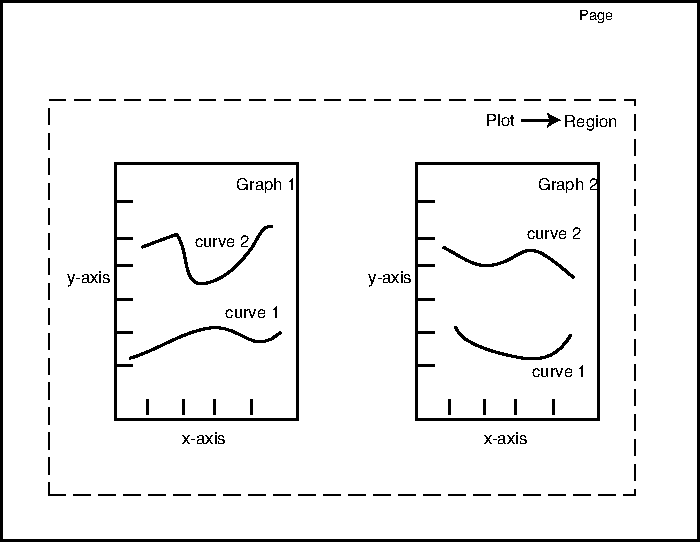
\includegraphics{plot.pdf}
  \caption[A plot has a collection of graphs.]
{A plot has a collection of graphs and a graph has a 
collection of curves. A plot becomes visible when it is associated
with some region on the page using the \vn{place} command. Note that
on the actual page the plot/region border is not visible.}
  \label{f:plot}
\end{figure}

Some definitions:
  \vspace*{-3ex}
\begin{description}
\index{curve|hyperbf}
\item[Curve] \Newline
A \vn{curve} is a set of (x,y) points to be plotted.
\index{graph|hyperbf}
\item[Graph] \Newline
A \vn{graph} consists of horizontal and vertical axes along with a set
of \vn{curve}s that are plotted within the graph. 
\index{plot|hyperbf}
\item[Plot] \Newline
A \vn{plot} is essentially a collection of \vn{graphs}.
\index{page|hyperbf}
\item[Page] \Newline
The \vn{page} refers to the X11 window where graphics are displayed or the 
corresponding printed graphics page.
\index{region}
\item[Region] \Newline
The \vn{page} is divided up into a number of rectangles called
\vn{regions}. \vn{Regions} may overlap.
\end{description}

\index{template plot}\index{region}\index{place command}
\index{plot!initialization file}
The plot initialization file (cf.~Chapter~\ref{c:init}) defines a set of \vn{template
plots}. A \vn{template} defines what type of data is to be plotted (orbit, beta function,
etc.), how many \vn{graphs} there are, what the scales are for the \vn{graph} axes, how
the \vn{graph}s are laid out, etc.  The plot initialization file also defines a set of
\vn{region}s within the \vn{page}. Any \vn{template plot} can be placed in any
region. Using the \vn{place} command (see Chapter~\ref{c:command} for a full descriptions
of all commands) one can assign a particular \vn{template plot} to a particular region for
plotting.  The relationship between \vn{region}, \vn{plot}, \vn{graph}, and \vn{curve} is
shown graphically in Figure~\ref{f:plot}.

Figures~\ref{f:plot.page1} and \ref{f:plot.page2} show examples of a plot
\vn{page}. Figure~\ref{f:plot.page1} was generated by defining two regions called \vn{top}
and \vn{bottom} in the plot initialization file. The \vn{top} region was defined to cover
the upper half of the \vn{page} and the \vn{bottom} region was defined to cover the bottom
half. \vn{Template plots} were defined to plot phase and orbit data from a defined set of
detector elements in the lattice. Each \vn{template plot} defined two graphs which in both
cases where assigned the names \vn{x} and \vn{y}. The orbit \vn{template plot} was placed
in the \vn{top} region and the phase \vn{template plot} was placed in the \vn{bottom}
region. The horizontal axis numbering is by detector \vn{index}.  Displayed plots are
referred to by the \vn{region} name (\vn{top} and \vn{bottom} in this case). Individual
graphs and curves are referred to using the nomenclature \vn{region.graph.curve}. Thus, in
this example, the horizontal orbit graph would be referred to as \vn{top.x}.  Using the
\vn{set plot}, \vn{set graph}, or \vn{set curve} commands (\sref{s:set}) one can then
specify what \vn{components} are plotted. ``\vn{component}'' refers to \vn{measured},
\vn{reference}, \vn{model}, \vn{base}, and/or \vn{design} data (\sref{s:plot.data}).
Notice that the same \vn{template plot} can be assigned to different \vn{regions} and the
plots in different \vn{regions} can have different scales for their axes or different
\vn{components}. In the example in Figure~\ref{f:plot.page1}, the \vn{component} for the
\vn{top} plot is \vn{model} and for the \vn{bottom} plot it is \vn{model - design}.

Plots may be referred to by their template name or by the name of the region they are
placed in. For example, the orbit plot in Figure~\ref{f:plot.page1} may be referred to
using the region name (\vn{top}) or the template name (\vn{orbit}). A template may be
placed in multiple regions.  For example, you may wish to plot the \vn{model} data for the
orbit in one region and the \vn{design} data for the orbit in another region. In this case
the command \vn{scale orbit} would scale the plots in both regions while to scale the plot
in only one of the regions you would need to use the region name.

A graph of a plot is specified using the format \vn{plot_name.graph_name} where
\vn{plot_name} is a template or region name and \vn{graph_name} is the name of the
graph. For example, if the horizontal orbit graph of the \vn{orbit} plot is named \vn{x}
then it would be referred to as \vn{orbit.x} or \vn{top.x}. If a plot has only one graph,
the graph may be specified by just using the plot name.

A curve within a graph is specified using the format
\vn{plot_name.graph_name.curve_name}. If a graph has only one curve, the curve may be
specified using only the graph name \vn{plot_name.graph_name}. Additionally, if the there
is only one curve in a plot, the curve can be specified by just using the \vn{plot_name}.

The \vn{use}, \vn{veto}, \vn{restore}, and \vn{clip} commands are used to control what
data is used in fitting the model to the data in the optimization process (see
Chapter~\ref{c:opti}). The general rule is that these commands only affect measured and
reference data. If plotting \vn{model}, \vn{design} and/or \vn{base} data then the data
will be displayed irregardless. If plotting \vn{meas} and/or \vn{ref} data then the data
displayed will vary with these commands.  \vn{meas} or \vn{ref} data vetoed for display is
also vetoed for fitting.  However, measured data that is off the vertical or horizontal
scale may still be used by the optimizer unless vetoed with the \vn{veto} or \vn{clip}
command.  If there are data points off the vertical scale then ``**Limited**'' will appear
in the upper right-hand corner of the graph. If plotting measured data then these points
off scale will still be used by the optimizer.

The \vn{x_axis} and \vn{x_scale} commands are used to set the axis type and scale for each
graph. The axis type can be either \vn{index}, \vn{ele_index} or \vn{s} which corresponds
to the data index number, element index number and longitudinal position in the lattice
(from element 0) respectively.

Figure~\ref{f:plot.page2} shows another example of a plot \vn{page}.  In this case the
\vn{page} was generated by again defining two vertically stacked regions but in this case
the regions have different heights.  A \vn{template plot} with a single graph was placed
in the bottom most \vn{region}.  This \vn{graph} contains a \vn{key_table}.  A
\vn{key_table} is used in conjunction with \vn{single mode} and is explained in
Chapter~\sref{c:single}. A \vn{template plot} containing five \vn{graphs} was placed in
the uppermost region. The uppermost \vn{graph} of this \vn{template plot} contains a
\vn{lat_layout} which shows the placement of lattice elements.  What elements are
displayed in a \vn{lat_layout} and what shapes they are represented by is specified in the
initialization file. The horizontal scale is longitudinal position (\vn{s}).  The
remaining four graphs show dispersion and beta data from two different universes
representing the low energy and high energy transport in an energy recovery linac. The
individual data points here (hard to see in this example) have been slaved to the
\vn{lat_layout} and represent the beta and dispersion at the edges of the displayed
elements in the \vn{lat_layout}.

\begin{figure}
  \centering
  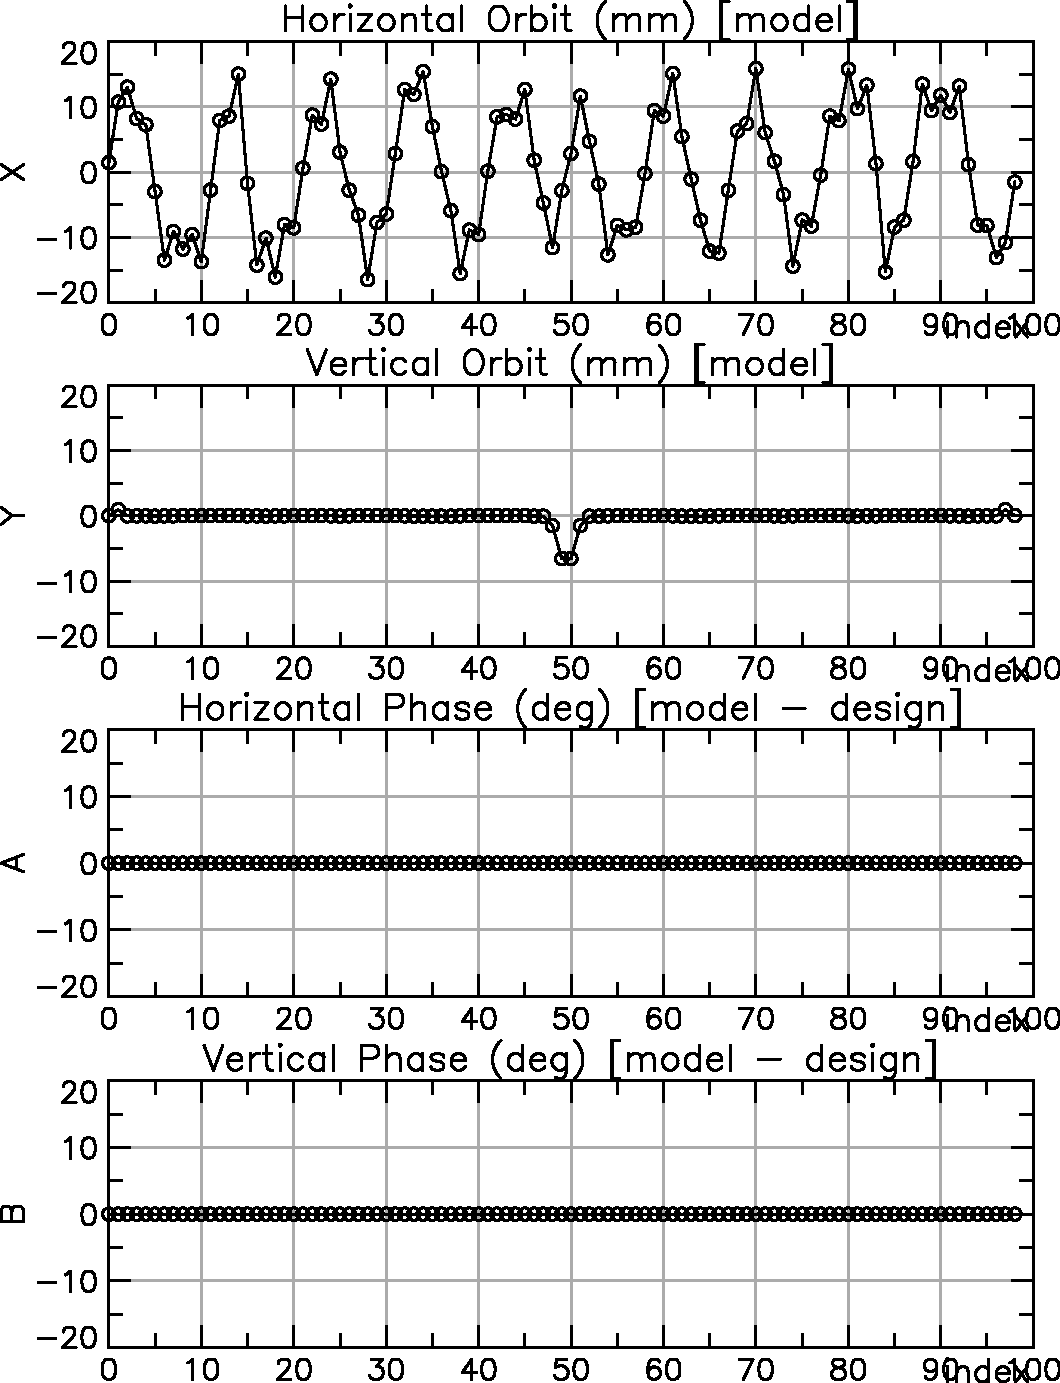
\includegraphics[width=5in]{plot-page1.pdf}
  \caption{Example of a plot page}
  \label{f:plot.page1}
\end{figure}

\begin{figure}
  \centering
  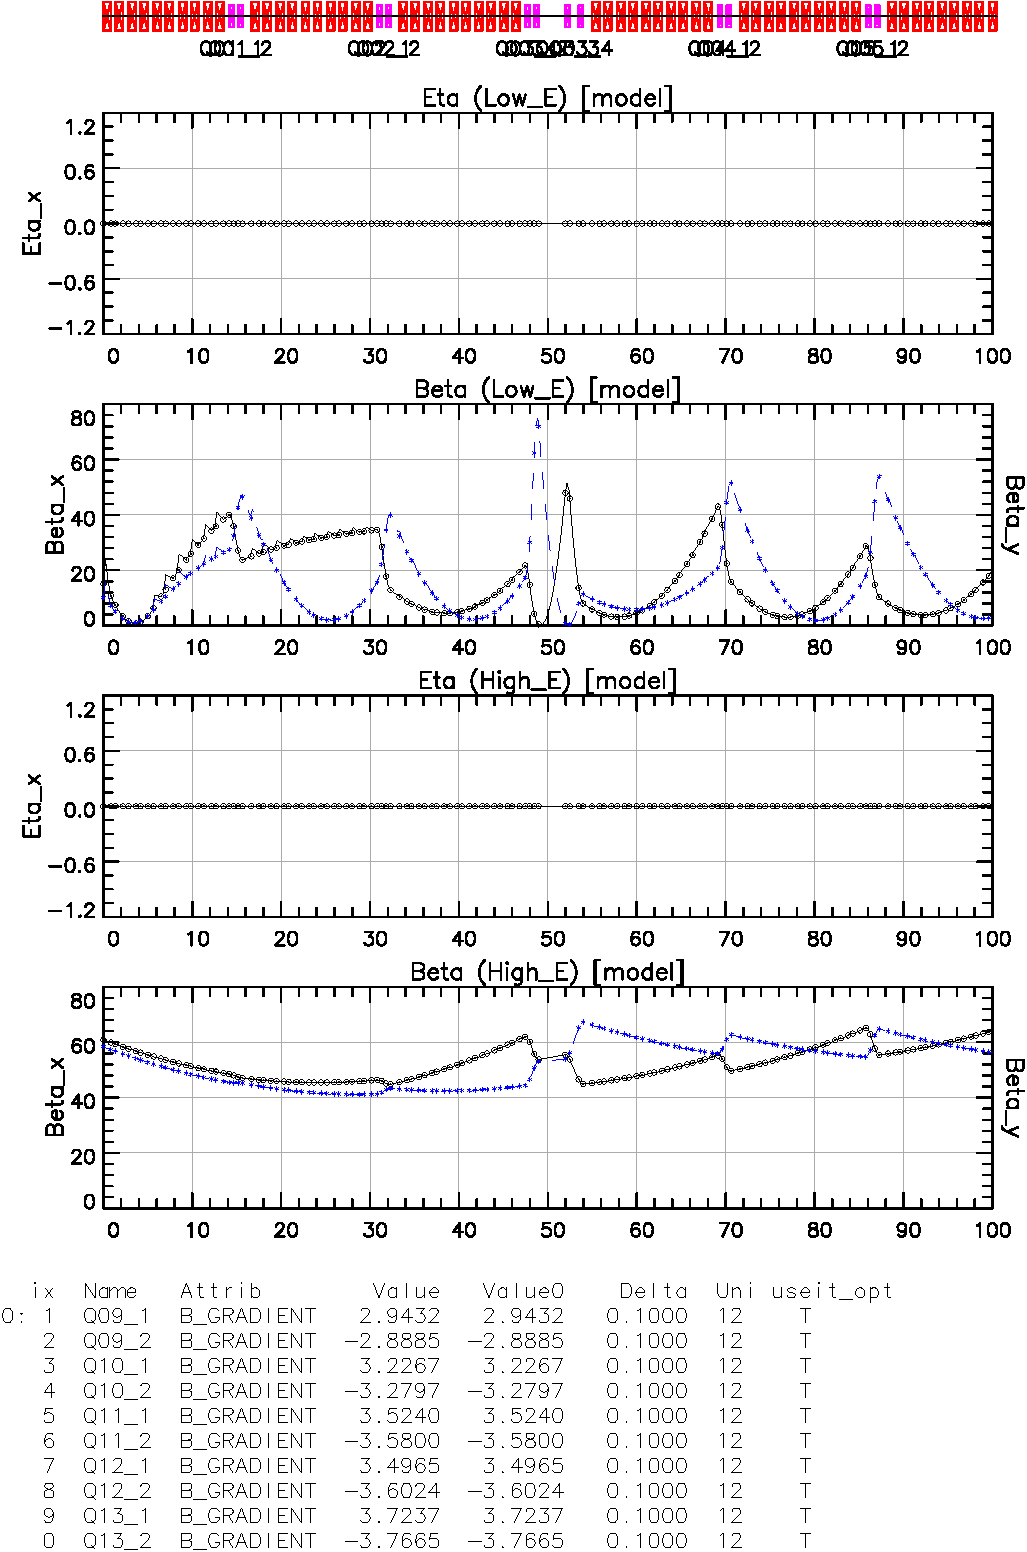
\includegraphics[width=5in]{plot-page2.pdf}
  \caption{Another example of a plot page.}
  \label{f:plot.page2}
\end{figure}

\vfill
\break

\chapter{Optimization: Lattice Correction and Design}
\label{c:opti}

\index{optimization|hyperbf}
\index{merit function}
This chapter covers the process of \vn{optimization} which involves minimization of a
\vn{Merit Function}. Optimization can be used to correct or to design lattices. Examples of \vn{lattice
corrections} include flattening the orbit and adjusting quadrupoles to correct the
measured betatron phase. \vn{Lattice design} involves creating a lattice that conforms to
a set of desirable properties. For example, requiring that the beta function in a certain
region never exceeds a given value. In this chapter,
Section~\sref{s:lattice.correction} presents the merit function in the context of lattice
corrections while Section~\sref{s:lattice.design} discuses the merit function in the
context of lattice design. Since the concepts used in \vn{lattice corrections} and
\vn{lattice design} are similar, \tao combines the two into one generalized process as
discussed in Section~\sref{s:generalized.design}.

%------------------------------------------------------------------------
\section{Lattice Corrections}
\label{s:lattice.correction}
\index{modeling data}
\index{lattice corrections}

\index{optimization!merit function}
Consider the problem of problem of modifying the orbit of a beam through a lattice to
conform to some desired orbit (typically a ``flat'' orbit running through the centers of
the quadrupoles). The process generally goes through three stages: First the orbit is
measured, then corrections to the steering elements are calculated and finally the
corrections are applied to the machine. Since these are necessarily machine specific, \tao
has no specific routines to measure orbits or to load steering corrections but they could
be implemented with some custom coding as discussed in Chapter~\sref{c:custom.tao}. What
\tao does, however, is to implement a generalized algorithm procedure for minimizing a
\vn{merit function} which can be used to calculate the corrections.  The idea is to vary a
set of variables (steerings in the case of an orbit correction) within the \vn{model}
lattice (\sref{s:universe}) with the aim to make the \vn{measured} \vn{data} (position
data for an orbit correction) correspond to the values as calculated from the \vn{model}
lattice.  Once the model lattice the \vn{model} and \vn{measured} data agree, the
difference between the \vn{model}, which represents the state of the machine when the
measurement is made, and the \vn{design}, which represents the desired state of the
machine, is used to calculate corrections. In the case of flattening an orbit, the
difference between the \vn{model} steering strengths and the \vn{design} steering
strengths (typically the \vn{design} steering strengths are zero) is what the real
steerings need to be changed by to flatten the orbit.

The merit function \vn{M} that is a measure of how well the data as calculated from the
\vn{model}, fits the measured data. \tao uses a merit function of the form
\Begineq
  {\cal M} \equiv 
    \sum_{i} w_i \, \bigl[ \delta D_i \bigr]^2 + 
    \sum_{j} w_j \, \bigl[ \delta V_j \bigr]^2
  \label{m1}
\Endeq
where
\begin{align}
  \delta D &= \data\_\model - \data\_\meas \CRNO
  \delta V &= \var\_\model  - \var\_\meas
  \label{dd1}
\end{align}
\vn{data_model} is the data as calculated from the \vn{model} and \vn{data_meas} is the
measured data. \vn{var_model} is the value of a variable in the \vn{model} and
\vn{var_meas} is the value as measured at the time the data was taken (for example, by
measuring the current through a steering and using a calibration factor to calculate the
kick) and the sum \vn{j} runs over all variables that are allowed to be varied to minimize
\vn{M}. The second term in the merit function prevents degeneracies (or near
degeneracies) in the problem which would allow \tao to find solutions where
\vn{data_model} matches \vn{data_measured} with the \vn{var_model} having ``unphysical''
values (values far from \vn{var_meas}). The weights $w_i$ and $w_j$ need to be set
depending upon how accurate the measured data is relative to how accurate the calibrations
for measuring the \vn{var_meas} values are. With the second term in the merit function,
the number of constraints (number of terms in the merit function) is always larger than
the number of variables and degeneracies can never occur.

In a correction one wants to change the machine variables so that the
measured data corresponds to the design values \vn{data_design}. Thus
the change in the data that one wants is
\begin{example}
  data_change = data_design - data_meas
\end{example}
Once a fit has been made, and presuming that the \vn{data_model} is
reasonably close to the \vn{data_meas} this data change within the
\vn{model} lattice can be accomplished by changing the variables by
\begin{example}
  var_change = var_design - var_model
\end{example}
This assumes the system is linear. For many situations this is true
since typically \vn{var_change} is ``small''. Since the variables have
a measured value of \vn{var_meas} the value that the variables should
be set to is
\begin{example}
  var_final = var_meas + (var_design - var_model)
\end{example}
Notice that the fitting process is independent of the \vn{design}
lattice. It is only when calculating the corrections to the
variables that the \vn{design} lattice plays a role. 

Sometimes it is desired to fit to changes in data as opposed to the absolute value of the
data. For example, when closing an orbit bump knob what is important is the difference in
orbits before and after the bump knob is varied. Designating one of these orbit the
\vn{reference}, the appropriate deltas to be used in \Eq{m1} are
\begin{align}
  \delta D &= (\data\_\model - \data\_\design) - (\data\_\meas - \data\_\reference) \CRNO
  \delta V &= (\var\_\model - \var\_\design)   - (\var\_\meas - \var\_\reference)
  \label{dd2}
\end{align}
where \vn{data_ref} and \vn{var_ref} refer to the reference measurement.  These deltas
are acceptable if the reference data is taken with the machine reasonably near the
design setup so that nonlinearities can be ignored. If this is not the case then the
fitting becomes a two step process: The first step is to fit the \vn{model} to the
\vn{reference} data using the deltas of \Eq{dd1}. The \vn{base} lattice is then set
equal to the \vn{model} lattice. The second step is to fit the model using the deltas
\begin{align}
  \delta D &= (\data\_\model - \data\_\base) - (\data\_\meas - \data\_\reference) \CRNO
  \delta V &= (\var\_\model - \var\_\base)   - (\var\_\meas - \var\_\reference)
  \label{dd3}
\end{align}

Control of what data and what variables are to be used in the fitting
process is controlled by the \vn{use}, \vn{veto}, \vn{restore}, and
\vn{clip} commands.

%------------------------------------------------------------------------
\section{Lattice Design}
\label{s:lattice.design}
\index{optimization!lattice design}
\index{optimization!constraints}

Lattice design is the process of calculating \vn{variable} strengths
to meet a number of criteria called constraints. For example, one
constraint could be that the beta function in some part of the lattice
not exceed a certain value. In this case we can proceed as was done
for lattice corrections and use \Eq{m1}. In this case, the deltas
are computed to limit values to some range so a typical delta
would be of the form
\Begineq
  \delta D \; \text{or} \; \delta V = 
    \begin{cases}
    \mbox{model} - \mbox{limit}  & \mbox{model $>$ Limit} \\
    0                            & \mbox{otherwise}
    \end{cases}
\Endeq
or a constraint is used to keep the \vn{model} at a certain value so
the form of the constraint would be
\Begineq
    \delta D \; \text{or} \; \delta V = \mbox{model} - \mbox{target}  
\Endeq
Here \vn{model} is the value as calculated from the \vn{model}
lattice. \vn{target} and \vn{limit} are given numbers. Part of the
optimization process is in deciding what the values should be for any
\vn{target} or \vn{limit}.

%------------------------------------------------------------------------
\section{Generalized Design}
\label{s:generalized.design}
\index{optimization!generalized merit function}

The form of the deltas used in the merit function is determined by two global logicals
called \vn{opt_with_ref} and \vn{opt_with_base} (\sref{s:globals}) as shown in
Table~\ref{t:delta}.
\begin{table}[ht] 
\centering 
{\tt
\begin{tabular}{lll} \toprule
  \vn{Opt_with_ref} & \vn{Opt_with_base} & \vn{delta} \\ \midrule
  F & F & model - meas                \\
  T & F & model - meas + ref - design \\
  F & T & model - meas - base         \\
  T & T & model - meas + ref - base   \\
\bottomrule
\end{tabular}
} 
\caption{The form of \vn{delta}}  
\label{t:delta}
\end{table}
An exception occurs when using a \vn{common base lattice}
(\sref{s:cbl}). In this case, the common universe does not have base
or reference values associated with it. Thus all data and variables
that are associated with the common universe calculate their
\vn{delta} as if both \vn{opt_with_ref} and \vn{opt_with_base} were
set to \vn{False}.

Another exception occurs with data when the datum value cannot be
computed (\sref{s:datum.opt}). In this case, the datum's \vn{invalid} value
is used for the \vn{delta}. This is useful, for example, in a linear
lattice when the particle trajectory results in the particle being lost.

The \vn{Non-Zero-Condition} needed for a non--zero $D_i$ is dependent
upon the \vn{merit_type} of the datum (\sref{s:data.anatomy}).
There are five \vn{merit_type} constraint
types as given in Table~\ref{t:con.type}.
\begin{table}[ht]
\centering
{\tt
\begin{tabular}{|l|l|l|} \toprule
  {\it Merit\_Type}       & {\it Non-zero-Condition} \\ \midrule
  \vn{target}            & Any \vn{delta}   \\
  \vn{min}, \vn{abs_min} & \vn{delta} $<$ 0 \\
  \vn{max}, \vn{abs_max} & \vn{delta} $>$ 0 \\
\bottomrule
\end{tabular}
}
\caption{Constraint Type List.}
\label{t:con.type}
\end{table}
\index{optimization!optimize with reference}

For variables, the form of the terms $V_i$ is determined by its \vn{merit_type}.
Here the \vn{merit_type} may be:
\begin{example}
  target
  limit
\end{example}
A \vn{target} \vn{merit_type} for a variable is the same as for
datum. In this case \vn{model} is just the value of the variable.
A \vn{limit} \vn{merit_type} has the form
\Begineq
  \delta V = 
    \begin{cases}
    \mbox{model} - \mbox{high\_lim}  & \mbox{model} > \mbox{high\_lim} \\
    \mbox{model} - \mbox{low\_lim}   & \mbox{model} < \mbox{low\_lim} \\
    0                                & \mbox{Otherwise}
    \end{cases}
\Endeq
The default \vn{merit_type} for a variable is \vn{limit}.

Note: when doing lattice design \vn{opt_with_ref} and
\vn{opt_with_base} are both set to \vn{False} and the \vn{target} and
\vn{limit} values are identified with \vn{Meas}.

When optimizing a storage ring, If the ring is unstable so that the
twiss parameters, closed orbit, etc. cannot be computed, the
contribution to the merit function from the corresponding datums is
set to zero. This tends to lower the merit function and in this case
an optimizer will never leave the unstable region. To avoid this,
an \vn{unstable_ring} constraint (\sref{s:data.types}) must be set.

To see a list of constraints when running \tao use the \vn{show
constraints} command (\sref{s:show}). To see how a particular variable
or datum is doing use the \vn{show data} or \vn{show variable}
commands.  See \sref{s:datum.opt} for details on how datums are
chosen to be included in an optimization.

%------------------------------------------------------------------------
\section{Variable Limits and Optimization}
\label{s:limit}

High (\vn{high_lim}) and low (\vn{low_lim}) limiting values can be set
for any variable (\sref{s:init.var}). If not explicitly set,
\vn{high_lim} defaults to $10^30$ and \vn{low_lim} defaults to
$-10^30$. When running the optimizer, if the (model) value of a
variable is outside of the range set by the limits, the value will be
set to the value of the appropriate limit and the variable's
\vn{good_user} parameter (\sref{c:var}) is set to False so that no
further variation by the optimizer is done.

If the parameter \vn{global%var_limits_on} (\sref{s:globals}) is set
to \vn{False}, limit settings are ignored. 

By default, any variable value outside of the limit range will
reset. Even those variables that are not varied by the optimizer. If
this behavior is not desired, the parameter
\vn{global%only_limit_opt_vars} may be set to \vn{True}.  If this is
done, only variables that the optimizer is allowed to vary are
restricted.

The \vn{global%optimizer_var_limit_warn} parameter controls
whether a warning is printed when a variable value goes past a limit.
The default is \vn{True}.

%------------------------------------------------------------------------
\section{Optimizers in Tao}
\label{s:tao.opti}
\index{optimization!optimizer}

The algorithm used to vary the \vn{model} variables to minimize \vn{M} is called an
\vn{optimizer}. In \vn{command line mode} the \vn{run} command is used to invoke an
\vn{optimizer}. In \vn{single mode} the \vn{g} key starts an optimizer. In both modes the
period key (\vn{``.''}) stops the optimization (however, the
\vn{global%optimizer_allow_user_abort} parameter (\sref{s:globals}) can be set to False to
prevent this). Running an optimizer is also called ``fitting'' since one is trying to get
the \vn{model} data to be equal to the \vn{measured} data. With orbits this is also called
``flattening'' since one generally wants to end up with an orbit that is on--axis.

The optimizer that is used can be defined when using the \vn{run} command but
the default optimizer can be set in the \tao input file by setting the
\vn{global%optimizer} component (\sref{s:globals}).

When the optimizer is run in \tao, the optimizer, after it initializes
itself, takes a number of \vn{cycles}. Each cycle consists of changing
the values of the variables the optimizer is allowed to change. The
number of steps that the optimizer will take is determined by the
parameter \vn{global%n_opti_cycles} (\sref{s:globals}). When the
optimizer initializes itself and goes through
\vn{global%n_opti_cycles}, it is said to have gone through one
\vn{loop}. After going through through \vn{global%n_opti_loops} loops,
the optimizer will automatically stop.  To immediately stop the
optimizer the period key \vn{``.''} may be pressed. Note: In
\vn{single_mode} (\sref{c:single}), \vn{n_opti_loops} is ignored and
the optimizer will loop forever.

There are currently three optimizers that can be used: 
  \begin{description}
  \index{lm optimizer}
  \item{\vn{lm}} \Newline
\vn{lm} is an optimizer based upon the Levenburg-Marquardt algorithm
as implemented in \vn{Numerical Recipes}\cite{b:nr}. This algorithm
looks at the local derivative matrix of \vn{dData/dVariable} and takes
steps in variable space accordingly. The derivative matrix is
calculated beforehand by varying all the variables by an amount set by
the variable's \vn{step} component (\sref{s:init.var}). The \vn{step}
size should be chosen large enough so that round-off errors will not
make computation of the derivatives inaccurate but the step size
should not be so large that the derivatives are effected by
nonlinearities. By default, the derivative matrix will be recalculated
each \vn{loop} but this can be changed by setting the
\vn{global%derivative_recalc} global parameter (\sref{s:globals}). The
reason to not recalculate the derivative matrix is one of time.
However, if the calculated derivative matrix is not accurate (that is,
if the variables have changed enough from the last time the matrix was
calculated and the nonlinearities in the lattice are large enough),
the \vn{lm} optimizer will not work very well.  In any case, this
method will only find local minimum.
  \index{lmdif optimizer}
  \item{\vn{lmdif}} \Newline
The \vn{lmdif} optimizer is like the \vn{lm} optimizer except that it
builds up the information it needs on the derivative matrix by
initially taking small steps over the first \vn{n} cycles where \vn{n}
is the number of variables. The advantage of this is that you do not
have to set a \vn{step} size for the variables. The disadvantage is
that for \vn{lmdif} to be useful, the number of \vn{cycles} must be
greater than the number of variables. Again, like \vn{lm}, this method
will only find local minimum.
  \index{de optimizer}
  \item{\vn{de}} \Newline
The \vn{de} optimizer stands for \vn{differential
evolution}\cite{b:de}. The advantage of this optimizer is that it
looks for global minimum. The disadvantage is that it is slow to find
the bottom of a local minimum. A good strategy sometimes when trying
to find a global minimum is to use \vn{de} in combination with \vn{lm}
or \vn{lmdif} one after the other. One important parameter with the
\vn{de} optimizer is the \vn{step} size. A larger step size means that
the optimizer will tend to explore larger areas of variable space but
the trade off is that this will make it harder to find minimum in the
locally. One good strategy is to vary the \vn{step} size to see what
is effective. Remember, the optimal step size will be different for
different problems and for different starting points. The \vn{step}
size that is appropriate of the \vn{de} optimizer will, in general, be
different from the \vn{step} size for the \vn{lm} optimizer. For this
reason, and to facilitate changing the step size, the actual step size
used by the \vn{de} optimizer is the step size given by a variable's
\vn{step} component multiplied by the global variable
\vn{global%de_lm_step_ratio}. This global variable can be varied using
the \vn{set} command (\sref{s:set}). The number of trial solutions used 
in the optimization is
\begin{example}
  population = number_of_variables * global%de_var_to_population_factor
\end{example}
There are also a number of parameters that can be set that will affect
how the optimizer works. See Section~\sref{s:globals} for more
details.
  \index{svd optimizer}
  \item{\vn{svd}} \Newline
The \vn{svd} optimizer uses a singular value decomposition
calculation.  See the description of \vn{svdfit} from Numerical
Recipes\cite{b:nr} for more details. With the \vn{svd} optimizer, the
setting of the \vn{global%n_opti_cycles} parameter is ignored. One
optimization loop consists of applying svd to the derivative matrix to
locate a new set of variable values.  If the merit function decreases
with the new set, the new values are retained and the optimization
loop is finished. If the merit function increases, and if the global
variable \vn{global%svd_retreat_on_merit_increase} is True (the
default), the variables are set to the original variable settings. In
either case, an increasing merit function will stop the execution of
additional loops.

The \vn{global%svd_cutoff} variable can be used to vary the cutoff
that SVD uses to decide what eigenvalues are sigular. See the
documentation for the Numerical Recipes routine \vn{svdfit} for more
details.
  \end{description}

%------------------------------------------------------------------------
\section{Optimization Troubleshooting Tips}
\label{s:opt.trouble}
\index{optimization troubleshooting}

Optimizations can behave in strange ways. Here are some tips on how to diagnose problems.

The \vn{show optimizer} (\sref{s:show.optimizer}) command will show global parameters
associated with optimizations. This will show some of the parameters that can be 
varied to get better convergence. One quick thing to do is to increase the number of
optimization loops and/or optimization cycles:
\begin{example}
	set global n_opti_loops = ...
	set global n_opti_cycles = ...
\end{example}

One of the first things to check is the merit function, the top contributors can be seen
with the command \vn{show top10} (\sref{s:show.top10}). And individual contributions
can be viewed using the \vn{show variable} and \vn{show data} commands.

If using an optimizer that uses the derivative matrix (\vn{lm}, \vn{geodesic_lm} and 
\vn{svd} optimizers), The variable \vn{step} sizes that are used to calculate the derivative
should be checked to make sure that the \vn{step} is not too small so that roundoff is a problem
but yet not too large so that nonlinearities make the calculation inaccurate. One way to
check that the step size is adequate for a given variable is to vary the variable using
the command \vn{change var} (\sref{s:change}). This command will print out the the change
in the merit function per change in variable which can be compared to the derivatives 
as shown with the \vn{show top10 -derivative} (\sref{s:show.top10}) or the
\vn{show derivative} (\sref{s:show.derivative}) command.

%------------------------------------------------------------------------
\section{Common Base Lattice (CBL) Analysis}
\label{s:cbl}
\index{common base lattice}

Some data analysis problems involve varying variables in a both the
\vn{model} and \vn{base} lattices simultaneously. Such is the case
with Orbit Response Matrix (\vn{ORM}) analysis\cite{b:orm}. With
\vn{ORM}, the analysis starts with a set of difference orbits. A given
difference orbit is generated by varying a given steering by a known
amount and the steering varied is different for different difference
orbits. Typically, The number $N$ of difference orbits is equal to the
number of steering elements in the machine. In \tao, this will result
in the creation of $N$ universes, one for each difference
measurement. The \vn{model} lattice in a universe will correspond to
the machine with the corresponding steering set to what it was when
the data was taken. Conversely, the \vn{base} lattices in all the
universes all correspond to the common condition without any steering
variation.

In \tao, this arrangement is called \vn{Common Base Lattice}
(\vn{CBL}) analysis. To do a CBL analysis, the \vn{common_lattice}
switch must be set at initialization time (\sref{s:init.lat}).  With
\vn{CBL}, \tao will set up a \vn{``common''} universe with index 0.
The \vn{model} lattice of this common universe will be used as the
\vn{base} lattice for all universes. 

The variables (fit parameters) in a \vn{CBL} analysis can be divided
into two classes. One class consists of the parameters that were
varied to get the data of the different universes. With \vn{ORM},
these are the steering strengths. At initialization
(\sref{s:init.var}), variables must be set up that control these
parameters. A single variable will control that particular parameter in
a particular universe, that was varied to create the data for that
universe. 

The second class of variables consists of everything that is
to be varied in the common base lattice. With \vn{ORM}, this generally
will include such things as quadrupole and BPM error tilts, etc. That
is, parameters that did {\em not} change during data taking. The
\tao variables that are created for these parameters will control
parameters of the \vn{model} lattice in the common universe.

To cut down on memory usage when using \vn{CBL} (the number of data
sets, hence the number of universes, can be very large), \tao does
not, except for the common \vn{model} lattice, reserve separate memory
for each \vn{model} lattice. Rather, it reserves memory for a single
\vn{``working''} lattice and the \vn{model} lattice for a particular
universe is created by first copying the common \vn{base} lattice to
the \vn{working} lattice and then applying the variable(s) (a steering
in the case of \vn{ORM}) appropriate for that universe.  As a result,
except for the common \vn{model} lattice, it is not possible to vary a
parameter of a \vn{model} lattice unless that parameter has a \tao
variable that associated with it. The \vn{change} command
(\sref{s:change}) is thus restricted to always vary parameters in
the common \vn{model} lattice.

With \vn{CBL}, the \vn{opt_with_base} and \vn{opt_with_ref}
(\sref{s:generalized.design}) global logicals are generally set to
True. Since \vn{opt_with_base}, and \vn{opt_with_ref} do not make
sense when applied to the data in the common universe, The
contribution to the merit function from data in this universe is
always calculated as if \vn{opt_with_base} and \vn{opt_with_ref} were
set to False.

With \vn{opt_with_base} set to True, the \vn{base} value for a
datum is evaluated by looking for a corresponding datum in the common
universe and using its \vn{model} value. To simplify the bookkeeping,
it is assumed that the structure of the data arrays is identical from
universe to universe. That is, the \vn{show data} command gives
identical results independent of the default universe. 

\chapter{Wave Analysis}
\label{c:wave}

%----------------------------------------------------------------
\section{General Description}
\label{s:wave.general}

A ``wave analysis'' is method for finding isolated ``kick errors'' in
a machine by analyzing the appropriate data. Types of data that can be
analyzed and the associated error type is shown in
Table~\ref{t:wave0}.  

The analysis works on difference quantities. For example, the
difference between measurement and theory or the difference between
two measurements, etc. Orbit and vertical dispersion measurements are the
exception here since an analysis of, say, just an orbit measurement can
be considered to be the difference between the measurement and a
perfectly flat (zero) orbit.

\begin{table}[h]
\centering{\tt
\begin{tabular}{|l|l|} \hline
  {\it Measurement Type}  & {\it Error Type}           \\ \hline
  Orbit                   & Steering errors            \\ \hline
  Betatron phase          & Quadrupolar errors         \\ \hline
  Beta function           & Quadrupolar errors         \\ \hline
  Coupling                & Skew quadrupolar errors    \\ \hline
  Dispersion              & Sextupole errors           \\ \hline
\end{tabular}}
\caption[Wave measurement types.]
{Types of measurements that can be used in a wave analysis and the 
types of errors that can be diagnosed.}
\label{t:wave0}
\end{table}

\begin{figure}[t]
  \centering
  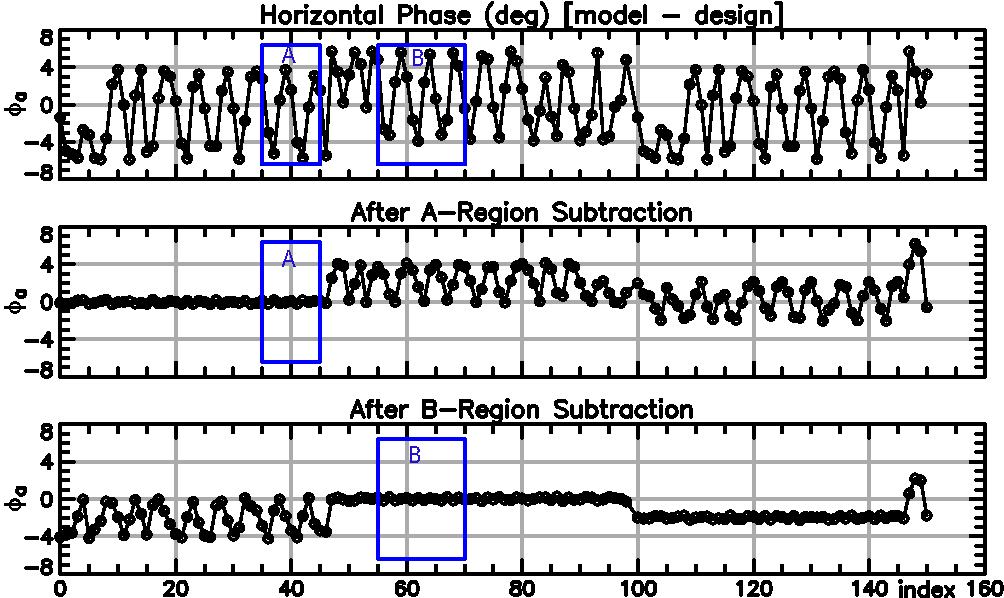
\includegraphics[width=6in]{wave.pdf}
  \caption[Example wave analysis.]
{Example wave analysis for betatron phase data.}
  \label{f:wave}
\end{figure}

The formulation of the wave analysis for quadrupolar and skew
quadrupolar errors is presented by Sagan\cite{b:wave}.  Although not
discussed in the paper, the wave analysis for orbit and dispersion
measurements is similar to the beta function analysis that is
presented. 

The wave analysis is similar for all the measurement types. How the
wave analysis works is illustrated in Figure~\ref{f:wave}.
Figure~\ref{f:wave}a shows the difference between \vn{model}
and \vn{design} values for the $a$-mode betatron phase for the Cornell's 
Cesr storage ring. In this example, one quadrupole in the model has 
been varied from it's design value. The horizontal axis is the detector index. 

For the wave analysis, two regions of the machine, labeled $A$ and $B$
in the figure, are chosen (more on this later). For each region in
turn, the data in that region is fit using a functional form that
assumes that there are no kick errors in the regions. 
For phase differences, this functional form is
\Begineq
  \delta phi(s) = D \, \sin(2 \, \phi(s) + phi_0) + C
  \label{xabps}
\Endeq
where $\phi$ is the phase
advance and the quantities $C$, $D$ and $\phi_0$ are varied to give the best
fit.  Once $C$, $D$, and $\phi_0$ are fixed, \Eq{xabps} can be evaluated at
any point. Figure~\ref{f:wave}b shows the orbit of \ref{f:wave}a
with the fit to the $A$ region subtracted off. Similarly,
Figure~\ref{f:wave}c shows the orbit of Figure~\ref{f:wave}a with
the fit to the $B$ region subtracted off. Concentrating on
Figure~\ref{f:wave}b, since there are no kick errors in the $A$
region, the fit is very good and hence the difference between the data
and the fit is nearly zero. Moving to the right from the $A$ region in
Figure~\ref{f:wave}b, this difference is nearly zero up to where the
assumption of no kick errors is violated. That is, at the location of
the quadrupole error  near detector 47. Similarly, since there are no kick errors
in region $B$, the difference between the data and the $B$ region fit
is nearly zero in Figure~\ref{f:wave}c and this remains true moving leftward
from region $B$ up to the quadrupole near detector 47.

By taking the fitted values for $C$, $D$, and $\phi_0$ for the regions $A$
and $B$, the point between the regions where the kick is generated and
the amplitude of the kick can be calculated. This calculation is
similar to that used to find quadrupolar errors from beta
data\ref{f:wave}. The one difference is a factor of 2 that appears
in the beta calculation due to the fact that a freely propagating beta
wave oscillates at $2\phi(s)$. 

The success of the wave analysis in finding a kick error depends upon
whether there are regions of sufficient size on both sides of the kick
that are kick error free. That is, whether the kick error is
``isolated''. The locations of the $A$ and $B$ regions are set by the
user and the general strategy is to try to find, by varying the
location of the regions, locations where the data is well fit within
the regions. The data is well fit if the difference between data and
fit is small compared to the data itself. If there are multiple
isolated kick errors, then each error in turn can be bracketed and
analyzed. If there are multiple errors so close together that they
cannot be resolved, this will throw off the analysis, but it may still
be possible to give bounds for the location where the kicks are at and
an ``effective'' kick amplitude can be calculated.

For circular machines, to be able to analyze kicks near the beginning
or end of the lattice, the wave analysis can be done by ``wrapping''
the data past the end of the lattice for another 1/2 turn. This is
illustrated in Figure~\ref{f:wave}. In the Cesr machine, there are
approximately 100 detectors labeled from 0 to 99.  The detectors from
100 to 150 are just the detectors from 0 to 50 shifted by 100. Thus,
for example, the detector labeled 132 in the figure is actually
detector 32.

%----------------------------------------------------------------
\section{Wave Analysis in Tao}
\label{s:wave.tao}

Performing a wave analysis in \tao is a three step process:
\begin{example}
  1) Plot the data to be analyzed.
  2) Use the \vn{wave} command to select the data.
  3) Use the \vn{set wave} command to vary the fit regions.
\end{example}

In general, the accuracy of the wave analysis depends upon the
accuracy with which the beta function and phase advances are known in
the baseline lattice used. \tao uses the \vn{model} lattice for the
baseline. If possible, One strategy to improve the accuracy of the
wave analysis is first use a measurement to calculate what the
quadrupole strengths in the \vn{model} lattice should be. Possible
measurements that can give this information include an orbit response
matrix (ORM) analysis, fits to beta or betatron phase measurements, etc.

%----------------------------------------------------------------
\subsection{Preparing the Data} 
\label{ss:wave.data}

At present (due to limited manpower to do the
coding), the wave analysis is restricted to data that is stored in a
\vn{d1_data} array (\sref{c:data}). That is, the plotted curve to be
analyzed must have its \vn{data_type} parameter set to
\vn{``data''} (\sref{s:init.data}). The possible data types that
can be analyzed are:
\begin{example}
  orbit.x, orbit.y
  beta.a,  beta.b
  phase.a, phase.b
  eta.x, eta.y
  cbar.11, cbar.12, cbar.21      ! Analysis not possible for cbar.21
  ping_a.amp_x, ping_a.phase_x
  ping_a.sin_y, ping_a.cos_y
  ping_b.amp_y, ping_b.phase_y
  ping_b.sin_x, ping_b.cos_x
\end{example}
The curve to be analyzed must be visible. Any combination of data
components may be used:. "meas", "meas-ref", "model", etc.

If data from a circular machine is being analyzed, the data is wrapped
past the end of the lattice for another 1/2 turn. The translation from
the data index in the wrapped section to the first 1/2 section of the
lattice is determined by the values of \vn{ix_min_data} and
\vn{ix_max_data} of the \vn{d1_data} array under consideration
(\sref{s:init.data}):
\begin{example}
  index_wrap \(\longrightarrow\) index_wrap - (ix_max_data - ix_min_data + 1)
\end{example}
For example, for the Cesr example in the previous section,
\vn{ix_min_data} was 0 and \vn{ix_max_data} was 99 to the translation
was
\begin{example}
  index_wrap \(\longrightarrow\) index_wrap - 100
\end{example}

%----------------------------------------------------------------
\subsection{Wave Analysis Commands and Output}
\label{ss:wave.cmd.out}

The \vn{wave} command (\sref{s:wave}) sets which plotted data curve
is used for the wave analysis. The \vn{set wave} command (\sref{s:set}) 
is used for setting the $A$ and $B$ region locations. Finally the 
\vn{show wave} command (\sref{s:show}) prints analysis results. 

Example wave analysis output with \vn{show wave}:
\begin{example}
  ix_a:  35  45
  ix_b:  55  70
  A Region Sigma_Fit/Amp_Fit:     0.018
  B Region Sigma_Fit/Amp_Fit:     0.015
  Sigma_Kick/Kick:    0.013
  Sigma_phi:          0.019
  Chi_C:              0.037 [Figure of Merit]

  Normalized Kick = k * l * beta [dimensionless]
     where k = quadrupole gradient [rad/m^2].
  After Dat#     Norm_K       phi
         46      0.0705    30.431
         49      0.0705    33.573
         53      0.0705    36.715
\end{example}
This output is for analysis of betatron phase data but the output for
other types of data is similar.  The first two lines of the output
show where the $A$ and $B$ regions are. The next two lines show
$\sigma_{a}/A_a$ and $\sigma_{b}/A_b$ where $\sigma_a$ and $\sigma_b$
are given by Eq.~(42) of Sagan\cite{b:wave} and 
\Begineq
  A_a \equiv \sqrt{\xi_a^2 + \eta_a^2}
\Endeq
with a similar equation for $A_b$. $\sigma_{a}/A_a$ and
$\sigma_{b}/A_b$ are thus a measure of how well the data is fit in the
$A$ and $B$ regions with a value of zero being a perfect fit and a
value of one indicating a poor fit. Notice that a poor fit of one of
the regions may simply be a reflection that the wave amplitude being
there. The next three lines of the output are $\sigma_{\delta
k}/\delta k$, $\sigma_\phi$, and $\xi_C$, and are given by Eq.~(39),
(43), and (44) respectively of \cite{b:wave}. The last three lines of
the analysis tell where the wave analysis predicts the kicks are and
what the normalized kick amplitudes are. Thus the first of these three
lines indicates that the kick may be somewhere after the location of
datum \#46 (but before the location of datum \#47), The normalized
quadrupole kick amplitude is 0.0705, and the betatron phase at the
putative kick is 30.431 radians.

\chapter{Tao Initialization}
\index{Initialization}
\label{c:init}

\tao is customized for specific machines and specific calculations
using input files and custom software routines. Writing custom
software is covered in the programmer's guide section. This chapter
covers the input files.

In general, the input files tell \tao:
\begin{example}
  * What the "standard" variables should be.
  * What the "standard" data is.
  * What to plot and where to plot it.
\end{example}

Example initialization files can be found in the \tao distribution in
the directory
\begin{example}
  tao/examples
\end{example}

%-----------------------------------------------------------------
\section{Format}
\label{s:format}

Initialization parameters are read in from a file using Fortran
namelist input. Fortran namelist breaks up the input file into
blocks. The first line of a namelist block starts with an ampersand
``\&'' followed by the block identifying name. Variables are assigned
using an equal sign ``='' and the end of the block is denoted by a
slash ``/'' For example:
\begin{example}
  &namelist_block_name
    var1 = 0.123   ! exclamation marks are used for comments
    var2 = 0.456
  /
\end{example}
Variables that have default values can be omitted from the block.  The
order of the variables inside a block is irrelevant except if the
same variable appears twice in which case the last occurrence is determinative.
In between namelist blocks all text is ignored. Inside a block comments may be
included by using an exclamation mark ``!''.

Care must be taken when setting arrays in a namelist as the following example
shows:
\begin{example}
  &namelist_name
    var_array(8:11) = 34             ! Only sets var_array(8)
    var_array(8:11) = 34 34 81 81    ! OK. Sets all 4 values
    var_array(8:11) = 34, 34, 81, 81 ! OK. Same as above
    var_array(8:11) = 34, 34,        ! Lines may be continued ...
                      81, 81         !   ... like this.
    var_array(8:11) = 2*34 2*81      ! Equivalent to the preceding examples
    var_array(8:)   = 2*34 2*81      ! Also equivalent
    var_array(1:2) = 1 2 3           ! Error: Too many RHS values.
    string_arr = '1st' "2nd" '3rd'   ! Setting a string array.
    string_arr(1:3) = 1st 2nd 3rd    ! Same as above. [Not accepted by all compilers.]
    string_arr(1:3) = 1st,2nd,3rd    ! Same as above. [Not accepted by all compilers.]
    string_arr = 'A B' "2/" "&"      ! Quotes needed here.
  /
\end{example}
The first line to set the \vn{var_array} may look like it is setting 
the four values \vn{var_array(8:11)} but the general rule is that with \vn{n}
values on the RHS, only \vn{n} values in the array are set. Notice the notation
\vn{n*number} does not denote multiplication but instead can be used to denote
multiple values. Also note that the compiler may be picky about blanks so 
that ``2*34'' will be accepted but ``2 * 34'' may not.

For string input it is always best to use quotes. Some compilers will
accept strings without quotes. Even those that do will generally not
accept strings with special characters.  Thus the following characters
should not be used in unquoted strings:
\begin{example}
  Blank or Tab character.
  Period if it is the first character in the string.
  &   ,   /    !   %   *   (   )   =   ?   '   "
\end{example}
Note: While there are exceptions, in general \tao string variables are
case sensitive.

Logical variables should be set to \vn{T} or \vn{TRUE} when true and
\vn{F} or \vn{FALSE} when false. This is case insensitive. It is
possible to use the words \vn{.true.} and \vn{.false.} for logicals,
however this may not always work. The reason for this is that a
variable that is documented to be a logical may actually be a string
variable! In this case a beginning period will cause problems. Why use
string variables? Without going into detail, string variables are used
in place of logical variables when \tao needs to know if the variable
has been explicitly set.

%-----------------------------------------------------------------
\section{Beginning Initialization}
\index{Initialization!beginning}
\label{s:init.global} 

\index{tao_start}\index{tao.init}\index{lattice_file}
\index{data_file}\index{var_file}\index{plot_file}
\index{single_mode_file}\index{startup_file}\index{startup_single_mode}
\index{beam_file}\index{hook_init_file}
The initialization starts with the \tao initialization file. The default name for
this file is \vn{tao.init} (See \sref{s:command.line}).
The first namelist block read in from this initialization file is a 
\vn{tao_start} namelist. This block is optional (in which case the defaults
are used).  This namelist contains the variables:
\begin{example}
  &tao_start
    beam_file          = "<file_name>"  ! Default = Tao initialization file.
    building_wall_file = "<file_name>"  ! No Default.
    data_file          = "<file_name>"  ! Default = Tao initialization file.
    var_file           = "<file_name>"  ! Default = Tao initialization file.
    plot_file          = "<file_name1> \{<file_name2>\} ..."  
                                       ! Default = Tao initialization file.
    single_mode_file   = "<file_name>"  ! Default = Tao initialization file.
    startup_file       = "<file_name>"  ! Default = "tao.startup"
    hook_init_file     = '<file_name>'  ! Default = 'tao_hook.init'
    init_name          = "<init_name>"  ! Default = "Tao"
  /
\end{example}
Rule: A file name obtained from the \tao initialization file (as opposed to
being present on the command line) is always relative to the directory
that the \tao initialization file lives in. Example: If \tao is started from
the system command line like:
\begin{example}
    tao -data data.cl -init ../tao.init
\end{example}
And if the \vn{tao_start} namelist in \vn{../tao.init} looks like:
\begin{example}
  &tao_start
    data_file = "dat.in"
    plot_file = "plot.in"
    var_file  = "/nfs/var.in"
  /
\end{example}
Then, relative to the current working directory, the files used will be
\begin{example}
  data_file: "data.cl"      ! Command line arguments have preference
  plot_file: "../plot.in"   ! Relative to ../tao.init.
  var_file:  "/nfs/var.in"  ! Absolute paths are never modified.
\end{example}

\vn{init_name} is for naming the initialization. This is useful to
distinguish between multiple initialization files with custom versions
of \tao. The other parameters specify which files to find the other
initialization namelists. The \vn{plot_file} variable can be an array
of plot files. 

The following sections describe each of these initialization namelists
and their locations are listed in table~\ref{t:init.files}. Note: If
\vn{plot_file} specifies multiple files, the \vn{tao_plot_page},
\vn{lat_layout_drawing} and \vn{floor_plan_drawing}
namelists are taken from the first file on the list. All files,
however, can contain \vn{tao_template_plot} and
\vn{tao_template_graph} namelists.

\index{tao_design_lattice}\index{tao_params}
\index{tao_beam_init}\index{tao_var}\index{tao_d2_data}
\index{tao_d1_data}\index{tao_plot_page}\index{tao_template_plot}
\index{tao_template_graph}\index{lat_layout_drawing}
\index{floor_plan_drawing}
\begin{table}[ht]
\centering {\tt
\begin{tabular}{|l|l|l|l|} \hline
  {\it Namelist} & {\it File Name} & {\it Initialized here}  & {\it Section} \\ \hline
  \vn{lat_layout_drawing}        & \vn{plot_file}$^*$ & Plotting      & \sref{s:layout.and.floor}     \\ \hline
  \vn{floor_plan_drawing}        & \vn{plot_file}$^*$ & Plotting      & \sref{s:layout.and.floor}     \\ \hline
  \vn{tao_beam_init}             & \vn{beam_file}     & Particle beam & \sref{s:beam.init}     \\ \hline
  \vn{tao_building_wall}         & \vn{building_wall_file} & Plotting & \sref{s:building.wall} \\ \hline 
  \vn{tao_design_lattice}        & "tao.init"  & lattice files        & \sref{s:init.lat}      \\ \hline
  \vn{tao_d1_data}               & \vn{data_file}     & Data          & \sref{s:init.data}     \\ \hline
  \vn{tao_d2_data}               & \vn{data_file}     & Data          & \sref{s:init.data}     \\ \hline
  \vn{tao_params}                & "tao.init"  & Global Variables     & \sref{s:globals}       \\ \hline
  \vn{tao_plot_page}             & \vn{plot_file}$^*$ & Plotting      & \sref{s:init.plot}     \\ \hline
  \vn{tao_template_graph}        & \vn{plot_file}     & Plotting      & \sref{s:init.plot}     \\ \hline
  \vn{tao_template_plot}         & \vn{plot_file}     & Plotting      & \sref{s:init.plot}     \\ \hline
  \vn{tao_var}                   & \vn{var_file}      & Variables     & \sref{s:init.var}      \\ \hline
\end{tabular}}
\break
$^*$This namelist taken from the first file in the {plot\_file} array.
\caption{Table of \vn{tao} Initialization Namelists.}
\label{t:init.files}
\end{table}

%-----------------------------------------------------------------
\section{Lattice Initialization}\index{initialization!lattice}
\label{s:init.lat} 

In the \vn{tao_start} namelist, the \vn{lattice_file} variable gives
the name of the file that contains the \vn{tao_design_lattice}
namelist. This namelist defines where the lattice input files are. The
variables that are set in the \vn{tao_design_lattice} namelist are:
\index{tao_design_lattice}\index{design_lattice}\index{design_lattice!file}
\index{design_lattice!parser}\index{n_universes}\index{common_lattice}
\begin{example}
  &tao_design_lattice
    n_universes        = <integer>      ! Number of universes. Default = 1.
    unique_name_suffix = "<string>"
    combine_consecutive_elements_of_like_name = <logical>
    common_lattice = <logical>                        ! Default = False
    design_lattice(i) = "<lattice_file>", \{"<lattice2_file>"\}
    design_lattice(i)%one_turn_map_calc = <logical>     ! Default = False
    design_lattice(i)%dynamic_aperture_calc = <logical> ! Default = False
  /
\end{example}

\vn{n_universes} is the number of universes to be created not counting
the possible common universe created when using \vn{CBL} analysis. The
default is 1.  \vn{design_lattice(i)} gives the lattice file name for
universe \vn{i}.  
The syntax for \vn{<lattice_file>} is:
\begin{example}
  \{<parser>::\}<lattice_file>\{\#reverse\}\{@<use_line>\}
\end{example}
Possible choices for the <parser> are:
\index{bmad}\index{xsif}\index{digested}
\begin{example}
  bmad      ! For a standard bmad lattice file. This is the default.
  xsif      ! For an xsif lattice file.
  digested  ! For a digested BMAD file.
\end{example}
If \vn{\#reverse} is present, tracking will be in the reverse direction from the end of
the lattice to the beginning. The sign of the charge of the tracked particle
will also be reversed. This is useful for simulating beams that go in the backward direction.

Example:
\begin{example}
  &tao_design_lattice
    n_universe = 4
    design_lattice(1) = "this.lat#reverse"  ! Default: Bmad format lattice file.
    design_lattice(2) = "xsif::that.lat", "floor_coords.bmad"
                                            ! XSIF file. For universe \#2 
    design_lattice(3) = "third.lat@my_line"     ! Specify a different line.
    design_lattice(3)%one_turn_map_calc = True  ! Calculate higher order maps.
  /
\end{example}
In this example, the lattice of universe 1 is given by the file
\vn{this.lat} and the lattice of universe 2 is given by the file
\vn{that.lat}. The \vn{"xsif::"} prefix for \vn{design_lattice(2)}
indicates that the xsif parser is to be used. Alternatively, a
\vn{".xsif"} suffix signals that a file uses the \vn{xsif}
format. 
\vn{design_lattice(2)} in the example also specifies a ``secondary
lattice file'' called \vn{floor_coords.bmad} which will be parsed
after the ``primary'' \vn{that.lat} file is read. This secondary
lattice file must only have statements that are valid post lattice
expansion.  See the \bmad manual manual for a discussion of lattice
expansion. A secondary lattice file must be in Bmad standard
format. This can be especially useful if \vn{lattice_file} is not a
bmad file. For example, a \vn{lattice2_file} can be used to set
non-zero floor coordinates to an XSIF lattice file. 

If there is no \vn{design_lattice} specified for a given universe then
the last \vn{design_lattice} is used. Thus, in the above example,
universes 4 use the same lattice as universe 3.

The \vn{design_lattice(i)%one_turn_map_calc} sets whether a
one-turn-map calculation for a ring using PTC will be done. If the
calculation is made, the \vn{normal.} data type is populated.  See
Eq.~\ref{normalform1} and Eq.~\ref{normalform2}. After startup, the
map calculation can be toggled on/off by using the \vn{set universe
one_turn_map_calc} command (\sref{s:set}).

The \vn{design_lattice(i)%dynamic_aperture} component sets whether the
dynamic aperture calculation (\sref{s:dynamicaperture}) will be
done. After startup, this calculation can be toggled on/off by
using the \vn{set universe dynamic_aperture_calc} command (\sref{s:set}).

Normally, a lattice file will specify which ``line'' will be used to
specify the lattice. Occasionally, it is convenient to override this
specification and to use a different line. To do this in \tao, the
name of the line to be used to specify the lattice can be appended to
the lattice file name. Thus, in the example above, universe 3 will
have the lattice specified by the line ``my\_line'' from the lattice
``third.lat''.

\vn{global%combine_consecutive_elements_of_like_name} takes a lattice
and combines all pairs of consecutive elements that have the same name
and attributes. Why is this useful? Some programs, not based on \bmad,
cannot generate the Twiss parameters inside the element. If the Twiss
parameters at the center of an element are desired, a lattice where the
element has been split into two identical pieces is needed. This,
however, makes tasks like setting up lattice optimization
cumbersome. Note: The recombination of like elements happens when the
lattice is read in during initialization.

\vn{unique_name_suffix} is used to append a unique character string to
element names that are not unique. \vn{unique_name_suffix} uses
element list format (\sref{s:ele.list.format}). The class is used to
restrict which elements can have their names changed. The \vn{name}
part is used as a suffix. This suffix must have a single \vn{``?''}
character.  When this suffix is applied to an element's name, a unique
integer is inserted in place of the \vn{``?''}. For example, if
\vn{unique_name_suffix} is \vn{"quad::\#\#?"}, and if the following
quadrupoles are in the lattice:
\begin{example}
        QA    QB    QX    QA    QB     QB
\end{example}
then after initialization, the names will be:
\begin{example}
        QA##1  QB##1  QX    QA##2  QB##2   QB##3
\end{example}
Using \vn{\#\#?"} as the suffix is convenient since it corresponds
to the \bmad standard convention for distinguishing elements of the
same name. See the \bmad manual for more details on this.

Setting \vn{aperture_limit_on} to \vn{False} will turn off the
aperture limits set in all lattices. This overrides the setting of
\vn{parameter[aperture_limit_on]} in a lattice file.

The \vn{common_lattice} switch can be used when there is a baseline
lattice that is common to all universes. See \sref{s:cbl} for more
details.

%-----------------------------------------------------------------
\section{Initializing Globals}\index{initialization!globals}
\label{s:globals} 

Global variables are initialized in the \vn{data_and_var_file} using a
namelist block named \vn{tao_params} The syntax of this block is:
\index{tao_params}\index{global}\index{bmad_com}\index{csr_param}\index{opti_de_param}
\begin{example}
  &tao_params
    global        = <tao_global_struct>     ! global parameters.
    bmad_com      = <bmad_com_struct>       ! Bmad global parameters.
    csr_param     = <csr_parameter_struct>  ! CSR global parameters.
    opti_de_param = <opti_de_param_struct>  ! de optimizer parameters.
  /
\end{example}
Example:
\begin{example}
  &tao_params
    global%optimizer = "lm"  ! Set the default optimizer.
  /
\end{example}

The \vn{tao_global_struct} structure contains \tao global parameters.
\index{y_axis_plot_dmin}\index{n_opti_cycles}\index{ix_key_bank}
\index{n_lat_layout_label_rows}\index{phase_units}
\index{bunch_to_plot}\index{random_seed}
\index{beam_random_engine}\index{beam_random_gauss_converter}
\index{track_type}\index{prompt_string}\index{Optimization!setting the optimizer}
\index{write_file}\index{var_limits_on}\index{only_limit_opt_vars}
\index{plot_on}\index{opt_with_ref}\index{opt_with_base}
\index{single_mode}\index{init_opt_wrapper}\index{lm_opt_deriv_reinit}
\index{label_lattice_elements}\index{label_keys}\index{derivative_recalc}
\index{init_plot_needed}\index{lattice_calc_on}\index{command_file_print_on}
\index{print_command}\index{default_init_file}\index{derivative_uses_design}
\index{current_init_file}\index{var_out_file}\index{draw_curve_off_scale_warn}
\begin{example}
type tao_global_struct
  real(rp) y_axis_plot_dmin = 1e-4    ! Minimum y_max-y_min allowed for a graph.
  real(rp) lm_opt_deriv_reinit = -1   ! Derivative matrix cutoff. -1 => ignore this.
  real(rp) de_lm_step_ratio = 1       ! Step sizes between DE and LM optimizers.
  real(rp) de_var_to_population_factor = 5 
  real(rp) svd_cutoff = 1e-5          ! SVD singular value cutoff limit.
  real(rp) random_sigma_cutoff = -1   ! Cut-off in sigmas.
  real(rp) merit_stop_value = -1      ! Value below which an optimizer will stop.
  integer n_opti_cycles = 20          ! number of optimization cycles
  integer n_opti_cycles = 1           ! number of optimization loops
  integer n_lat_layout_label_rows = 1 ! How many rows with a lat_layout
  integer phase_units = radians\$      ! Phase units on output.
  integer bunch_to_plot = 1           ! Which bunch to plot
  integer random_seed = 0             ! use system clock by default
  character(16)  random_engine = "pseudo"         ! Random number engine to use
  character(16)  random_gauss_converter = "exact" ! Uniform to gauss conversion method
  character(16)  track_type = "single"            ! "single" or "beam" 
  character(16)  prompt_string = "Tao"
  character(16)  optimizer     = "de"             ! optimizer to use.
  character(40)  print_command = "lpr"
  character(80)  var_out_file  = "var#.out"
  logical command_file_print_on = T     ! Toggle printing when using a command file.
  logical derivative_recalc = T         ! Recalc derivatives before each optimizer loop?
  logical derivative_uses_design = F    ! Derivative matrix uses the design lattice?
  logical disable_smooth_line_calc = F  ! Disable the plotting smooth line calc?
  logical draw_curve_off_scale_warn = T ! Display warning on graphs when any part of the 
                                        !   curve is out-of-bounds
  logical init_opt_wrapper = T
  logical init_plot_needed = T          ! reinitialize plotting?
  logical label_lattice_elements = T    ! For lat_layout plots
  logical label_keys = T                ! For lat_layout plots
  logical lattice_calc_on = T           ! Master switch.
  logical opt_with_ref = F              ! use reference data in optimization?
  logical opt_with_base = F             ! use base data in optimization?
  logical optimizer_var_limit_warn = T  ! Warn when vars reach a limit when optimizing?
  logical plot_on = T                   ! Do plotting?
  logical rf_on = F                     ! RF cavities on?
  logical svd_retreat_on_merit_increase = T    
  logical var_limits_on = T             ! Respect the variable limits?
  logical only_limit_opt_vars = F       ! Apply limits only if variable is used in optimization?
  logical single_step = F               ! Single step through a command file?
  logical optimizer_allow_user_abort = T ! See below.
end type
\end{example}

All global parameters can be changed from their initial value using
the \vn{set} command (\sref{s:set}).

  \begin{description}
  \item{\vn{global%command_file_print_on}} \Newline
The \vn{} switch controls whether printing is suppressed when a command file is called.

  \item{\vn{global%derivative_recalc}} \Newline
The \vn{global%derivative_recalc} logical determines whether the derivative matrix is
recalculated every optimization loop. The \vn{global%derivative_uses_design} logical
determines if the design lattice is used in the derivative matrix calculation instead of
the model lattice.

  \item{\vn{global%disable_smooth_line_calc}} \Newline
The \vn{global%disable_smooth_line_calc} is used to disable computation of the ``smooth
curves'' used in plotting.  This can be used to speed up \tao as discussed in
\sref{s:plot.data}.

  \item{\vn{global%lattice_calc_on}} \Newline
\vn{global%lattice_calc_on} controls whether lattice calculations are done. This switch is
useful in controlling unnecessary calculational overhead.  A typical scenario where this
switch is used involves first setting \vn{%lattice_calc_on} to \vn{False} (using the
\vn{set} command (\sref{s:set})), then executing a set of commands, and finally setting
\vn{%lattice_calc_on} back to \vn{True}. This saves some of the calculational overhead
that each command generates. Similarly, \vn{global%plot_on} can be toggled to save even
more time.

  \item{\vn{global%merit_stop_value}} \Newline
The \vn{global%merit_stop_value} establishes a point such that, during optimization, if
the merit function falls below that value, the optimization stops. If the value is
negative (the default), \vn{global%merit_stop_value} is ignored.

  \item{\vn{global%optimizer_allow_user_abort}} \Newline
Normally \vn{optimizer_allow_user_abort} defaults to True which allows the optimizer, when
it is run, to look for user input from the terminal (\sref{s:tao.opti}). If the user types
a period ``.'', the optimization is aborted cleanly. However, if \tao is started with
standard input redirected from a file (using the ``<'' character) \tao will not be able to
distinguish between input meant as a \tao command and input meant for aborting the
optimization. In this case, \vn{optimizer_allow_user_abort} will default to False so that
the optimizer will not do any checking.

  \item{\vn{Random Number Generation}} \Newline
Random number generation in \tao is divided into two categories: Random numbers used for
generating the initial coordinates of the particles in a beam and random numbers used for
everything else.  As explained below, there are four parameters that govern how random
numbers are generated. For beam particle generation, three of the four (everything except
the random number seed) are accessed through the \vn{beam_init} structure
(\sref{s:beam.init}). For everything else, these parameters are accessed through the
\vn{tao_global_struct}.

  \item{\vn{global%random_engine}} \Newline
\vn{global%random_engine} selects the algorithm used for generating the random
numbers. \vn{"pseudo"} causes \tao to use a pseudo-random number generator. \vn{"quasi"}
uses Sobel quasi-random number generator which generates a distribution that is smoother
then the pseudo-random number generator. \vn{"pseudo"} is the default.

  \item{\vn{global%random_gauss_converter}} \Newline
\vn{global%random_gauss_converter} selects the algorithm used in the conversion from a
uniform distribution to a Gaussian distribution.  \vn{"exact"} is an exact conversion and
\vn{"limited"} has a cut-off so that no particles are generated beyond. This cutoff is set
by \vn{global%random_gauss_cutoff}.

  \item{\vn{global%random_gauss_cutoff}} \Newline
See \vn{global%random_gauss_converter}.

  \item{\vn{global%random_seed}} \Newline
\vn{global%random_seed} sets the seed number for the pseudo-random number generator. A
value of \vn{0} (the default) causes the seed number to be picked based upon the system
clock. Use the \vn{show global} command to see what the seed number is.

  \item{\vn{global%rf_on}} \Newline
The rf cavities in circular lattices can be be toggled on or off using the
\vn{global%rf_on} switch. The default is False. Notice that with the RF off, the beam
energy will be independent of the closed orbit which is not the case when the RF is on.

  \item{\vn{global%single_step}} \Newline
For use with command files. If set True, this is equivalent to putting a "pause -1" after
each line in a command file. Useful for debugging.

  \item{\vn{global%track_type}} \Newline
The setting of the \vn{global%track_type} parameter can be
\begin{example}
  "single"
  "beam"
\end{example}
The \vn{"single"} setting is used when single particle tracking is desired and \vn{"beam"}
is used when tracking with a beam of particles. Note that with \vn{"single"} tracking,
synchrotron radiation fluctuations (but not damping) is always turned off.

  \item{\vn{global%var_limits_on}} \Newline
The \vn{global%var_limits_on} switch controls whether a variable's model value is limited
by the variable's \vn{high_lim} and \vn{low_lim} settings (\sref{s:init.var}). This is
particularly important during optimization. If a variable's model value moves outside of
the limits, the value is set at the limit and the variable's \vn{good_user} parameter is
set to \vn{False} so it will not be further varied in the optimization.

  \item{\vn{global%only_limit_opt_vars}} \Newline
The \vn{global%only_limit_opt_vars} switch controls whether only the variables being
optimized are limited or whether all variables are limited. The
\vn{global%optimizer_var_limit_warn} switch controls whether a warning is printed when a
variable value goes past a limit.

\end{description}

The \vn{bmad_com_struct} holds bmad global variables. 
\index{radiation_damping_on}\index{taylor_order}
\index{radiation_fluctuations_on}\index{sr_wakes_on}\index{lr_wakes_on}
\begin{example}
  type bmad_com_struct
    real(rp) max_aperture_limit = 1e3    
    real(rp) d_orb(6) = 1e-5  ! for the make_mat6_tracking routine
    real(rp) default_ds_step    = 0.2_rp    ! Integration step size.
    real(rp) significant_length = 1e-10     ! meter
    real(rp) rel_tol_tracking = 1e-8
    real(rp) abs_tol_tracking = 1e-10
    real(rp) rel_tol_adaptive_tracking = 1e-8   ! Adaptive tracking relative tolerance.
    real(rp) abs_tol_adaptive_tracking = 1e-10  ! Adaptive tracking absolute tolerance.
    real(rp) init_ds_adaptive_tracking = 1e-3   ! Initial step size
    real(rp) min_ds_adaptive_tracking = 0       ! Min step size to take.
    real(rp) fatal_ds_adaptive_tracking = 1e-8  ! particle lost if step size is below this.
    integer taylor_order = 3               ! 3rd order is default
    integer default_integ_order = 2        ! PTC integration order.
    integer ptc_max_fringe_order = 2       ! PTC max fringe order (2 => Quadrupole !).
                                           !   Must call set_ptc after changing.
    logical use_hard_edge_drifts = T       ! Insert drifts when tracking through cavity?
    logical sr_wakes_on = T                ! Short range wakefields?
    logical lr_wakes_on = T                ! Long range wakefields
    logical mat6_track_symmetric = T       ! symmetric offsets
    logical auto_bookkeeper = T            ! Automatic bookkeeping?
    logical space_charge_on = F            ! Space charge switch
    logical coherent_synch_rad_on = F      ! Longitudinal csr 
    logical spin_tracking_on = T           ! Do particle spin tracking
    logical radiation_damping_on = F       ! Damping toggle.
    logical radiation_fluctuations_on = F  ! Fluctuations toggle.
    logical conserve_taylor_maps = T       ! Enable bookkeeper to set ele%map_with_offsets = F?
    logical absolute_time_tracking_default = F  ! Default for lat%absolute_time_tracking
    logical rf_auto_scale_phase_default = T     ! Default for lat%rf_auto_scale_phase
    logical rf_auto_scale_amp_default = T       ! Default for lat%rf_auto_scale_amp
    logical use_ptc_layout_default = F          ! Default for lat%use_ptc_layout
  end type
\end{example}
See the \bmad manual for more details.

The \vn{csr_parameter_struct} holds global variables for the coherent
synchrotron radiation calculations. 
\begin{example}
  type csr_parameter_struct
    real(rp) ds_track_step = 0          ! Tracking step size
    real(rp) beam_chamber_height = 0    ! Used in shielding calculation.
    real(rp) sigma_cutoff = 0.1         ! Cutoff for the lsc calc. If a bin sigma
                                           !  is < cutoff * sigma_ave then ignore.
    integer n_bin = 0                   ! Number of bins used
    integer particle_bin_span = 2       ! Longitudinal particle length / dz_bin
    integer n_shield_images = 0         ! Chamber wall shielding. 0 = no shielding.
    integer ix1_ele_csr = -1            ! Start index for csr tracking
    integer ix2_ele_csr = -1            ! Stop index for csr tracking
    logical lcsr_component_on = T       ! Longitudinal csr component
    logical lsc_component_on = T        ! Longitudinal space charge component
    logical tsc_component_on = T        ! Transverse space charge component
    logical small_angle_approx = T      ! Use lcsr small angle approximation?
  end type
\end{example}
See the \bmad manual on the \vn{csr_parameter_struct} for more details. In \tao,
Besides setting the \vn{csr_parameter_struct} components, the following must
be done to enable CSR computations:
\begin{Itemize}
\item 
The \vn{global%track_type} (see above this section) must be set to \vn{"beam"} and the appropriate
beam initialization parameters (\sref{s:beam.init}) must be set.
\item 
The parameter \vn{bmad_com%coherent_synch_radiation} (see above this section) must be set to \vn{True}.
\item
In the \bmad lattice file, \vn{csr_calc_on} must be set for the elements where CSR tracking is to be
done (see the \bmad manual).
\end{Itemize}

The \vn{opti_de_param_struct} holds parameters that influence the behavior
of the \vn{de} optimizer (\sref{s:tao.opti})
\begin{example}
                         Default
  real(rp) CR               0.8    ! Crossover Probability.
  real(rp) F                0.8    !
  real(rp) l_best           0.0    ! Percentage of best solution used.
  logical  binomial_cross   False  ! IE: Default = Exponential.
  logical  use_2nd_diff     False  ! use F * (x_4 - x_5) term
  logical  randomize_F      False  !
  logical  minimize_merit   True   ! F => maximize the Merit func.
\end{example}
See the \bmad manual for more details.

If \vn{ix1_ele_csr} and \vn{ix2_ele_csr} are set, The effect of
coherent synchrotron radiation is only included in tracking in the
region from the exit end of the lattice element with index
\vn{ix1_ele_csr} through the exit end of the lattice element with index
\vn{ix2_ele_csr}. By restricting the CSR calculation,
the calculational time to track through a lattice is reduced.

See \sref{s:lattice.correction} for more details on
\vn{global%n_opti_cycles} and \vn{global%n_opti_loops}. 

%-----------------------------------------------------------------
\section{Initializing Particle Beams}\index{initialization!beams}
\label{s:beam.init}

A particle beam is initialized in the \vn{tao_beam_init} namelist block.
The syntax is as follows:
\index{tao_beam_init}\index{ix_universe}
\index{beam_init}\index{beam_init!a_norm_emit}
\index{beam_init!b_norm_emit}
\index{beam_init!dPz_dZ}\index{beam_init!center}\index{beam_init!sig_e}
\index{beam_init!sig_z}\index{beam_init!n_bunch}\index{beam_init!dt_bunch}
\index{beam_init!n_particle}\index{beam_init!bunch_charge}
\index{beam_init!renorm_center}\index{beam_init!renorm_sigma}
\index{beam_init!center_jitter}\index{beam_init!emit_jitter}
\index{beam_init!sig_z_jitter}\index{beam_init!sig_e_jitter}
\index{beam_init!polarization}\index{track_start}\index{track_end}
\begin{example}
  &tao_beam_init
    ix_universe                 = <integer>    ! Universe to apply to.
    beam0_file                  = <string>     ! File used in place of beam_init.
    beam_all_file               = <string>     ! File used in place of beam tracking.
    beam_saved_at               = "<ele_list>" ! Where to save the beam info.
    track_start                 = "<ele_name>" ! Element start tracking name or index.
    track_end                   = "<ele_name>" ! Element end tracking name or index.
    beam_init%distribution_type(3) = "<type>"  ! "ELLIPSE", "KV", "GRID", "" (default)
    beam_init%ellipse(3)%...    = ...          ! Parameters for an ellipse type distribution.
    beam_init%KV%...            = ...          ! Parameters for a KV distribution
    beam_init%grid(i)%...       = ...          ! Parameters for a grid distribution.
    beam_init%a_norm_emit       = <real>       ! A-mode energy normalized emittance
    beam_init%b_norm_emit       = <real>       ! B-mode energy normalized emittance
    beam_init%a_emit            = <real>       ! A-mode emittance
    beam_init%b_emit            = <real>       ! B-mode emittance
    beam_init%dPz_dZ            = <real>       ! Energy-Z correlation
    beam_init%center            = <real>*6     ! Bunch center offset relative to
                                               !   reference particle (BMAD coords)
    beam_init%sig_e             = <real>       ! e_sigma in dE/E0
    beam_init%sig_z             = <real>       ! Z sigma in m
    beam_init%n_bunch           = <integer>    ! Number of bunches
    beam_init%dt_bunch          = <real>       ! Time between bunches (meters)
    beam_init%n_particle        = <real>       ! Number of particles per bunch
    beam_init%bunch_charge      = <real>       ! charge per bunch (Coulombs)
    beam_init%renorm_center     = <logical>    ! Default is T
    beam_init%renorm_sigma      = <logical>    ! Default is F
    beam_init%center_jitter     = <real>*6     ! Bunch center rms jitter (meters)
    beam_init%emit_jitter       = <real>*2     ! Emittance rms jitter (\(d\epsilon/\epsilon\)) 
    beam_init%sig_z_jitter      = <real>       ! bunch length rms jitter (dz/z)
    beam_init%sig_e_jitter      = <real>       ! bunch energy spread rms jitter (dE/E)
    beam_init%spin%polarization = <real>       ! spin polarization (1.0 = 100%)
    beam_init%spin%theta        = <real>       ! spin orientation  (polar coordinate)
    beam_init%spin%phi          = <real>       ! spin orientation  (polar coordinate)
    beam_init%init_spin         = <logical>    ! Initialize the spin (default: False)
    beam_init%preserve_dist     = <logical>    ! Use the same particle distribution.
    beam_init%random_engine     = "pseudo"     ! random number engine to use
    beam_init%random_gauss_converter = "exact" ! Uniform to gauss conversion method
    beam_init%random_sigma_cutoff = 4.0        ! Cut-off in sigmas.
    beam_init%use_t_coords      = <logical>    ! Use time coords (for e_guns)?
    beam_init%use_z_as_t        = <logical>    ! Use time instead of z (for e_guns)?
  /
\end{example}
\vn{ix_universe} refers to the universe index.
See the \bmad documentation on the \vn{beam_init_struct} for what
the \vn{beam_init} parameters refer to. The charge per particle is set to
$\vn{bunch_charge} / \vn{n_particle}$ and is used when calculating wakefield
effects.

The emittances used construct to the beam's particle distribution can
be set using the energy normalized emittances \vn{%a_norm_emit} and
\vn{%b_norm_emit} or the unnormalized (``geometric'') \vn{%a_emit} and
\vn{%b_emit}. If not set, the emittances set in the lattice file
are used. These emittances are also used as the initial emittance in a
linear lattice for the emittance calculation using the radiation
integrals.

\label{s:beamfile}
The \vn{beam0_file} component specifies a beam data file (which can be
created with the \vn{write beam -at <ele_name>} command) which
contains a beam's particle coordinates which are to be used at the
start of the lattice.  Note: The file name can be overridden by using
the \vn{-beam0} argument on the command line
(\sref{s:command.line}). The file can either be in binary format
(binary files can be created by the \vn{write beam} command), or
written in ASCII. The ASCII file format is:
\begin{example}
  <ix_ele>         ! Lattice element index. This is ignored.
  <n_bunch>        ! Number of bunches.
  <n_particle>     ! Number of particles per bunch to use
  [bunch loop: ib = 1 to n_bunch]
    BEGIN_BUNCH    ! Marker to mark the beginning of a bunch specification block.
    <species_name> ! Species of particle
    <bunch_charge> ! Charge of bunch. 0 => Use <particle_charge>.
    <z_center>     ! z position at center of bunch.
    <t_center>     ! t position at center of bunch.
    [particle loop: Stop when END_BUNCH marker found]
      <x> <px> <y> <py> <z> <pz> <charge> <state> <spin_x> <spin_y> <spin_z> 
    [end particle loop]
    END_BUNCH      ! Marker to mark the end of the bunch specification block
  [end bunch loop]
\end{example}
Example:
\begin{example}
  0       ! ix_ele
  1       ! n_bunch
  25000   ! n_particle
  BEGIN_BUNCH
    POSITRON
    3.2E-9   ! bunch_charge
    0.0      ! z_center
    0.0      ! t_center
   -6.5E-3  9.6E-3 -1.9E-2  8.8E-3  2.2E-2 -2.4E-2  1.2E-13  1 1.0 0.0 0.0
    8.5E-3  5.5E-3  4.0E-2 -1.9E-2 -4.9E-3  2.1E-2  1.2E-13  1 1.0 0.0 0.0
    1.1E-2 -1.9E-2 -2.5E-2  1.0E-2 -1.8E-2 -7.1E-3  1.2E-13  1 1.0 0.0 0.0
   -3.4E-2 -2.7E-3 -4.1E-3  1.3E-2  1.3E-2  1.0E-2  1.2E-13  1 1.0 0.0 0.0
    6.8E-3 -4.5E-3  2.5E-3  1.4E-2 -2.3E-3  7.3E-2  1.2E-13  1 1.0 0.0 0.0
    1.2E-2 -9.8E-3  1.7E-3  6.4E-3 -9.8E-3 -7.2E-2  1.2E-13  1 1.0 0.0 0.0
    1.1E-2 -3.5E-4  1.2E-2  1.8E-2  5.4E-3  1.4E-2  1.2E-13  1 1.0 0.0 0.0
       ... etc. ...
  END_BUNCH
\end{example}

The first line of the file gives \vn{ix_ele}, the index of the lattice
element at which the distribution was created. This is ignored when
the file is Read. The second line gives \vn{<n_bunch>}, the number
of bunches. The third line gives \vn{n_particle} the number of
particles in a bunch. After this, there are \vn{<n_bunch>} blocks of
data, one for each bunch. Each one of these blocks starts with a
\vn{BEGIN_BUNCH} line to mark the beginning of the block and ends with
a \vn{END_BUNCH} marker line. In between, the first four lines give
the \vn{species} name, \vn{bunch_charge}, \vn{z_center}, and
\vn{t_center} values. The \vn{species} name may be one of:
\begin{example}
  positron  ! default
  electron
  proton
  antiproton
  muon
  antimuon
  photon
\end{example}

The lines following the \vn{t_center} line specify particle
coordinates. One line for each particle.
Only the first six number which are the phase space
coordinates need to be specified for each particle. if
\vn{<particle_charge>} is not present, or is zero, it defaults to
\vn{bunch_charge/n_particle}. The \vn{<state>} parameter
indicates whether a particle is alive or dead. Values are
\begin{example}
  1     ! Alive
  2-7   ! Dead
\end{example}

The particle spin is specified by $x$, $y$ and $z$ components.

The number rows specifying particle coordinates may be more then
\vn{<n_particle>}. In this case, particles will be discarded so that
the the beam has \vn{<n_particle>} particles. If
\vn{beam_init%n_particle}, if set in the \tao input file, this will
override the setting of \vn{<n_particle>} in the beam file.

Each particle has an associated \vn{<particle_charge>}. If
\vn{<bunch_charge>} is set to a non-zero value, the charge of all the
particles will be scaled by a factor to make the bunch charge equal
to \vn{<bunch_charge>}. Additionally, if \vn{beam_init%bunch_charge}
is set in the \tao input file, this will override the setting of
\vn{bunch_charge} in the beam file.

\index{change}\index{beam_start}\index{beam_init}
When the particle coordinates are read in from the \vn{beam0_file},
the centroid will be shifted by the setting of \vn{beam_init%center}.
To vary the centroid of the beam on the \tao command line, the \vn{set
beam_init%center} command (\sref{s:set}) can be used.

The \vn{beam_all_file} component specifies a beam data file (which can
be created with the \vn{write beam} command) which contains the
particle coordinates of the tracked beam at every element. This causes
\tao to use the data from the file in lieu of actual tracking. This
can be helpful when the time for \tao to track a bunch through the
lattice becomes long. The file name can be overridden by using the
\vn{-beam_all} argument on the command line
(\sref{s:command.line}). Note: \tao will set the variable
\vn{use_saved_beam_in_tracking} to \vn{True} to prevent actual
tracking.  Note: A \vn{beam_all_file} will supersede a \vn{beam0_file}

When there is no \vn{beam0_file} the Twiss parameters at the beginning
of the lattice are used in initializing the beam distribution.  For
circular lattices the Twiss parameters will be found from the closed
orbit, and the emittance will be calculated using the \bmad routine
\vn{radiation_integrals}.

\vn{track_start} and \vn{track_end} are used when it is desired to only track the beam
through part of the root lattice branch.  \vn{track_start} gives the starting element name
or index. Tracking will start at the exit end of this element so the beam {\em will not}
be tracked through this element. The tracking will end at the exit end of the lattice
element with name or index \vn{track_end}. The default, if \vn{track_start} and
\vn{track_end} are not present, is to track through the entire root lattice branch.
\vn{track_start} and \vn{track_end} is ignored for lattice branches other than the root
branch (branch 0).

If spin tracking is desired then \vn{beam_init%init_spin} must be set
to true.  If it is desired to use the exact same distribution of
particles for each time the beam is tracked then set
\vn{beam_init%preserve_dist} to True. Otherwise, a new random
distribution will be generated. The initialization routine does
attempt to renormalize the beam to the specified parameters,
nevertheless if tracking a small number of particles the distribution
is subject to small random fluctuations unless
\vn{beam_init%prserve_dist} is True.

\tao re-tracks the beam through the lattice every time a lattice
parameter is changed. For example, during optimizations or when the
\vn{set} command (\sref{s:set}) is used. For the re-tracking, the
particle distribution at the beginning of the lattice is fixed. That
is, the a new random distribution is {\emph not} generated. To force a
new distribution, use the \vn{reinitialize beam} command
(\sref{s:reinit}).

The default is single particle tracking. To turn on particle tracking the
\vn{global%track_type} parameter must be set to \vn{"beam"}. This can be placed in
the \vn{tao_params} namelist above, for example,
\begin{example}
  &tao_params
    global%optimizer = "lm"  ! Set the default optimizer.
    global%track_type = "beam"
  /
\end{example}

\vn{beam_saved_at} is used to specify at what elements the beam
distribution is to be saved at. The syntax used is
element list format as explained in \sref{s:ele.list.format}.
The \vn{BEGINNING} element (with index 0 in the lattice
list) and the last element are automatically saved.
\begin{example}
  &tao_beam_init
    beam_saved_at = "marker::m* *34w*" ! Save beam at all markers starting with "m"
                                      !   and all elements that have "34w" in their name. 
  /
\end{example}

The three random number generator parameters (\vn{%random_engine},
\vn{%random_gauss_converter}, and \vn{%random_sigma_cutoff}) used for
initializing the beam are set in the \vn{tao_global_struct}
(\sref{s:globals}). They may, however, be overridden for beam particle
generation by setting the corresponding parameters in the
\vn{beam_init} structure. That is, separate parameters may be setup
for beam particle generation verses everything else.  These parameters
are explained in Section~\sref{s:globals}.

%-----------------------------------------------------------------
\section{Initializing Variables}\index{initialization!variables}
\label{s:init.var} 

\vn{Variable}s are initialized using the \vn{tao_var} namelist. The
format for this is
\index{tao_var}\index{v1_var!name}\index{default_universe}
\index{default_attribute}\index{default_weight}\index{default_step}
\index{default_merit_type}\index{default_low_lim}\index{default_high_lim}
\index{ix_min_var}\index{ix_max_var}\index{var!name}
\index{var!ele_name}\index{var!attribute}\index{var!universe}
\index{var!weight}\index{var!step}\index{var!low_lim}
\index{var!high_lim}\index{var!merit_type}\index{var!good_user}
\index{use_same_lat_eles_as}\index{search_for_lat_eles}
\begin{example}
  &tao_var
    v1_var%name          = "<var_array_name>"  ! Variable array name.
    use_same_lat_eles_as = "<d1_name>"         ! Reuse a previous element list.
    search_for_lat_eles  = "<element_list>"    ! Find elements by name.
    default_universe     = "<integer>"         ! Universe variables belong in.
    default_attribute    = "<attribute_name>"  ! Attribute to control.
    default_weight       = <real>              ! Merit_function weight.
                                               ! default = 0.0
    default_step         = <real>              ! Small step value.
                                               ! default = 0.0
    default_merit_type   = "<merit_type>"      ! Sets how the merit is calculated.
                                               ! default = "limit"
    default_low_lim      = <real>              ! Lower variable value limit. 
                                               ! default = -1e30
    default_high_lim     = <real>              ! Upper variable value limit. 
                                               ! default =  1e30
    default_key_bound    = <logical>           ! Variables to be bound?
    default_key_delta    = <real>              ! Change when key is pressed.
    ix_min_var           = <integer>           ! Minimum array index.
    ix_max_var           = <integer>           ! Maximum array index.
    var(i)%ele_name      = "<ele_name>"        ! Element to be controlled.
    var(i)%attribute     = "<attrib_name>"     ! Attribute to be controlled.
    var(i)%universe      = "<uni_list>"        ! Universe containing variable to 
                                               !    be controlled. "*" => All.
    var(i)%weight        = <real>              ! Merit function weight.
    var(i)%step          = <real>              ! Small step size.
    var(i)%low_lim       = <real>              ! Lower variable value limit
    var(i)%high_lim      = <real>              ! Upper variable value limit
    var(i)%merit_type    = "<merit_type_name>" ! Sets how the merit is calculated.
    var(i)%good_user     = <logical>           ! Good optimization variable?
    var(i)%key_bound     = <logical>           ! Variable bound to a key
    var(i)%key_delta     = <real>              ! Change when key is pressed.
  /
\end{example}
Example:
\begin{example}
  &tao_var
    v1_var%name      = "v_steer"   ! vertical steerings
    default_universe  = "clone 2,3"
    default_attribute = "vkick"     ! vertical kick attribute
    default_weight    = 1e3
    default_step      = 1e-5
    ix_min_var        = 0
    ix_max_var        = 99
    var(0:99)%ele_name  = "v00w", "v01w", "v02w", "    ", "v04w", ...
  /
\end{example}

A \vn{tao_var} block is needed for each variable array to be defined.
\vn{v1_var%name} is the name of the array to be used with \tao
commands. The \vn{var(i)} array of variables has an index \vn{i} that
runs from \vni{ix_min_var} to \vni{ix_max_var}. A lattice element name
\vn{var(i)%ele_name} and the element's attribute to vary
\vn{var(i)%attribute} needs to specified. Not all elements need to
\vn{exist} and the element names of non--existent elements should be
undefined or set to a name with only spaces in it. For those variables
where \vn{var(i)%attribute} is not specified in the namelist the
\vn{default_attribute} will be used.

\vn{var(i)%key_bound} and \vn{var(i)%key_delta} are used to bind
variables to keys on the keyboard. The default values for these
parameters are set by \vn{default_key_bound} and
\vn{default_key_delta}. If not set, \vn{default_key_bound} is set to
\vn{False} and \vn{default_key_delta} is set to \vn{0}.
See~\sref{s:key.bind} for more details.

\vn{var(i)%step} establishes what a ``small'' variation of the
variable is. This is used, for example, by some optimizers when
varying variables. If \vn{var%step(i)} is not given for a
particular variable then the default \vn{default_step} is
used. 

\vn{var(i)%good_user} is a logical that the user can toggle when
running \tao (\sref{c:var}). The initial default value of
\vn{%good_user} is True.

\vn{var(i)%universe} gives the universe that the lattice element lives
in. Multiple universes can be specified using a comma delimited list.
For example:
\begin{example}
  var(10)%universe = "2, 3"
\end{example}
If \vn{var(i)%universe} is not present, or is blank, the value of
\vn{default_universe} is used instead. If both \vn{var(i)%universe} and
\vn{default_universe} are not present or blank then all universes are assumed.
In addition to a number (or numbers), 
\vn{default_universe} can have values:
\index{gang}\index{clone}
\begin{example}
  "gang"     -- Multiple universe control (default).
  "clone"    -- Make a var array block for each universe.
\end{example}
\vn{"gang"} means that each variable will control the given attribute
in each universe simultaneously. \vn{"clone"} means that the array of
variables will be duplicated, one for each universe.  To differentiate
variables from different universes \vn{_u<n>} will be appended to each
\vn{v1_var%name} where \vn{<n>} is the universe number.  For example,
if \vn{v1_var%name} is \vn{quad_k1} then the variable block name for
the first universe will be \vn{quad_k1_u1}, 
second universe will be \vn{quad_k1_u2}, etc. With \vn{"clone"},
individual \vn{var(i)%universe} may not be set in the namelist. The
default if both \vn{default_universe} and all \vn{var(i)%universe} are
not given is for \vn{default_universe} to be \vn{"gang"}. Examples:
\begin{example}
  default_universe = "gang"        ! Gang all universes together.
  default_universe = "gang 2, 3"   ! Gang universes 2 and 3 together.
  default_universe = "2, 3"        ! Same as "gang 2, 3".
  default_universe = "clone 2, 3"  ! Make two var arrays. 
                                   !   One for universe 2 and one for universe 3. 
\end{example}

\vn{var(i)%weight} gives the weight coefficient for the contribution
of a variable to the merit function.  If not present then the default
weight of \vn{default_weight} is used.  \vn{var(i)%low_lim} and
\vn{var(i)%high_lim} give the lower and upper bounds outside of which
the value of a variable should not go. If not present
\vn{default_low_lim} and \vn{default_high_lim} are used. If these are
not present as well then by default
\begin{example}
  low_lim  = -1e30
  high_lim =  1e30
\end{example}
\vn{var(i)%merit_type} determines how the merit contribution is calculated.
Possible values are:
\index{limit}\index{target}
\begin{example}
  "limit"       ! Default
  "target"      
\end{example}
For details on \vn{limit} and \vn{target} constraints see Chapter~\ref{c:opti}
on Optimization.

If elements in the \vn{var} array do not exist the corresponding
\vn{var%ele_name} should be left blank. Lists of names can be reused
using the syntax:
\index{use_same_lat_eles_as}
\begin{example}
  use_same_lat_eles_as = "<d1_name>"     ! Reuse a previous element list.
\end{example}
For example:
\begin{example}
  &tao_var
    v1_var%name     = "quad_tilt"  
    default_attribute = "tilt"
    ...
    use_same_lat_eles_as = "quad_k1"
  /
\end{example}

\index{search_for_lat_eles}
Instead of specifying a list of lattice element names for \vn{var(:)%ele_name}, 
\tao can be told to search for the elements by name using the syntax:
\begin{example}
   search_for_lat_eles = "{-no_grouping} <element_list>"  
\end{example}
Where \vn{<element_list>} is a list of elements using the element list format
(\sref{s:ele.list.format}). The searching will
automatically exclude any superposition and multipass slaves elements.
If the \vn{-no_grouping} flag is not present, the default behavior
is that all matched elements with the same name are grouped under a single
variable. That is, a single variable can control multiple elements.
On the other hand, if the \vn{-no_grouping} flag is present, each
element will be assigned an individual variable.  For example:
\begin{example}
  search_for_lat_eles = "sbend::b*"
\end{example}
will search for all non-lord bend lattice elements whose names begins
with \vn{"B"} followed by any set of characters. In this example, if,
for example, two bends have the name, say "bend0", then a single variable will be
set up to control these two bends.

Note: \vn{search_for_lat_eles} and \vn{use_same_lat_eles_as} cannot be
used together.

%-----------------------------------------------------------------
\section{Initializing Data and Constraints}
\index{initialization!data}\index{initialization!constants}
\label{s:init.data} 

A set of data (\sref{c:data}) is initialized using a \vn{tao_d2_data}
namelist block and one or more \vn{tao_d1_data} namelist blocks. The
format of the \vn{tao_d2_data} namelist is
\index{tao_d2_data}
\index{d2_data!name}
\index{Universe}
\index{default_merit_type}
\index{n_d1_data}
\begin{example}
  &tao_d2_data
    d2_data%name = "<d2_name>"          ! d2_data name.
    universe     = "<list>"             ! Universes data belong in.
                                        !   "*" => all universes (default).
    default_merit_type = "<merit_type>" ! Sets how the merit is calculated.
    n_d1_data          = <integer>      ! Number associated d1_data arrays.
  /
\end{example}
For example:
For example:
\begin{example}
  &tao_d2_data
    d2_data%name = "orbit"
    universe     = "1,3:5"  ! Apply to universes 1, 3, 4, and 5
    n_d1_data    = 2
  /
\end{example}
A \vn{tao_d2_data} block is needed for each \vn{d2_data} structure
defined. The \vn{d2_data%name} component gives the name of the
structure. The \vn{universe} component gives a list of the universes
that the data is associated with. A value of \vn{"*"} means that a
\vn{d2_data} structure is set up in each universe. Ranges of universes
can be specified in the list using a \vn{:}.

The \vn{default_merit_type} component determines how the merit
function terms are calculated for the individual datum
points. Possibilities are:
\index{target}\index{max}\index{min}
\index{abs_max}\index{abs_min}
\begin{example}
  "target"
  "max"
  "min"
  "abs_max"
  "abs_min"
\end{example}
See Chapter~\ref{c:opti} on optimization for more
details.

The associated \vn{tao_d1_data} namelists must come directly after
their associated \vn{tao_d2_data} namelist.  The \vn{n_d1_data}
parameter in the \vn{tao_d2_data} namelist defines how many
\vn{d1_data} structures are associated with the \vn{d2_data}
structure. For each \vn{n_d1_data} structure there must be a
\vn{tao_d1_data} namelist which has the form:
\index{tao_d1_data}\index{ix_d1_data}\index{d1_data!name}
\index{default_data_type}\index{default_weight}\index{ix_min_data}
\index{ix_max_data}\index{data!name}\index{data!data_type}
\index{data!ele_name}\index{data!ele_ref_name}\index{data!ele_start_name}\index{data!merit_type}
\index{data!meas}\index{data!weight}\index{data!good_user}
\index{data!ix_bunch}\index{use_same_lat_eles_as}\index{search_for_lat_eles}
\begin{example}
  &tao_d1_data
    ix_d1_data             = <integer>           ! d1_data index
    use_same_lat_eles_as   = "<d1_name>"         ! Reuse previous element list.
    search_for_lat_eles    = "<element_list>"    ! Find elements by name.
    d1_data%name           = "<d1_name>"         ! d1_data name.
    default_data_type      = <type_name>         ! Eg: orbit.x, e_tot, etc...
    default_weight         = <real>              ! Merit function weight. Dflt: 0.0
    default_data_source    = "<source>"          ! "lat" (dflt), "data", "var", or "beam". 
    ix_min_data            = <integer>           ! Minimum array index.
    ix_max_data            = <integer>           ! Maximum array index.
    datum(j)%data_source    = "<source>"         ! "lat" (dflt), "data", "var", or "beam". 
    datum(j)%data_type      = "<type_name>"      ! Eg: "orbit.x", etc.
    datum(j)%ele_name       = "<ele_name>"       ! Lattice element name.
    datum(j)%ele_start_name = "<ele_start_name>" ! Start element name.
    datum(j)%ele_ref_name   = "<ele_ref_name>"   ! Reference element names.
    datum(j)%merit_type     = "<merit_type>"     ! Sets how the merit is calculated.
    datum(j)%meas           = "<real>  "         ! Datum "measured" value
    datum(j)%weight         = "<weight>"         ! Merit function weight.
    datum(j)%good_user      = <logical>          ! Use for optimization and plotting?
    datum(j)%ix_bunch       = <integer>          ! Bunch index. Dflt: 0 = all bunches.
    datum(j)%eval_point     = "<where>"          ! "beginning", "center", or "end" (dflt).
    datum(j)%s_offset       = <real>             ! Default: 0.
  /
\end{example}
For example:
\begin{example}
  &tao_d1_data
    ix_d1_data        = 1 
    d1_data%name      = "x"  
    default_weight    = 1e6
    ix_min_data       = 0
    ix_max_data       = 99
    datum(0:)%ele_name = "DET_00W", " ", "DET_02W", ...
  /
\end{example}
Alternatively, one can specify a datum in a single line. For example, 
\begin{example}
  &tao_d1_data
    ix_d1_data        = 1 
    d1_data%name      = "t"  
    !           data_      ele_ref  ele_start ele     merit    meas   weight good
    !           type       name     name      name    type     value         user ..
    datum( 1) = "beta.a"   "S:2.3"  ""       "Q16_1"  "max"     30    0.1     T  ...
    datum( 2) = "phase.b"  "Q09_1"  "B22"    "Q16_1"  "max"     30    0.1     T  ...
    datum( 3) = "floor.x"  ""        ""      "end"    "target"   3    0.01    T  ...     
    datum( 4) = "floor.x"  "B1"      ""      "B2"     "target"   3    0.01    T  ...     
    ... etc. ...
  /
\end{example}
When specifying data one line at a time, the columns are
\begin{example}
  data_type
  ele_ref_name
  ele_start_name
  ele_name
  merit_type
  meas_value
  weight
  good_user
  data_source
  eval_point
  s_offset
  ix_bunch
\end{example}
Default values will be used if an individual line does not include all columns.

\vn{ix_min_data} and \vn{ix_max_data} give the bounds for the
\vn{datum(i)} structure array that is associated with the \vn{d1_data}
structure. \vn{datum(:)%ele_name} gives the lattice element names
associated with the data points.

\vn{datum(i)%good_user} is a logical that the user can toggle when
running \tao (\sref{s:data.anatomy}). The initial default value of
\vn{%good_user} is True.

A range of elements can be specified by giving an \vn{ele_start_name} that
is not a blank string. Thus, in the above example, the value of
\vn{datum(2)} is the maximum horizontal beta in the range between the
end of element \vn{B22} to the end of element \vn{Q16_1}. Elements
can be specified by name (Eg: \vn{Q16_1}) or by longitudinal position
using the notation \vn{"S:<s_distance>"}. This will match to the
element whose longitudinal position at the exit end is closest to
\vn{<s_distance>}.

\index{data_source}
\index{default_data_source}
The \vn{datum(:)%data_source} component specifies where the data is 
coming from. Possible values are:
\begin{example}
  "beam"        ! Value is from multiparticle beam tracking.
  "data"        ! Used with expressions.
  "lat"         ! Value is from the lattice.
  "var"         ! Used with expressions.
\end{example}
With \vn{%data_source} set to \vn{"beam"}, the particular bunch that the data is extracted
from can be specified via \vn{datum(:)%ix_bunch}.  The default is \vn{0} which combines
all the bunches for the datum calculation.  If the \vn{%data_source} is not set, the value
of the \vn{default_data_source} is used. If both \vn{%data_source} and
\vn{default_data_source} are not specified, \vn{"lat"} is the default. A \vn{%data_source}
of \vn{"data"} or \vn{"var"} establishes the default data source for evaluating
expressions (see \vn{"expression:"} in \sref{s:data.types}).

If elements in the \vn{data} array do not exist the corresponding
\vn{data%ele_name} should be left blank. Lists of names can be reused
using the syntax:
\index{use_same_lat_eles_as}
\begin{example}
  use_same_lat_eles_as = "<d1_name>"     ! Reuse previous element list.
\end{example}
For example:
\begin{example}
  &tao_d1_data
    ix_d1_data       = 2
    d1_data%name     = "y"  
    ...
    use_same_lat_eles_as = "orbit.x"
  /
\end{example}

\index{search_for_lat_eles}
\tao can search for the elements in the lattice to be associated with 
each data type by using the syntax:
\begin{example}
   search_for_lat_eles = "\{-no_lords\} \{-no_slaves\} <element_list>"
\end{example}
\vn{<element_list>} specifies elements using the standard element list
format (\sref{s:ele.list.format}). The \vn{-no_lords} and
\vn{-no_slaves} switches, if present, are used to restrict the counting
of lord or slave elements. The \vn{-no_lords} switch excludes all group,
overlay, and girder elements. The \vn{-no_slaves} switch vetoes
superposition or multipass slave elements. For example:
\begin{example}
  search_for_lat_eles = "-no_lords sbend::b*
\end{example}
This will search for all non-lord bend lattice elements whose names
begins with \vn{"B"} followed by any set of characters.
\vn{search_for_lat_eles} and \vn{use_same_lat_eles_as} cannot be used
together.

\index{data!data_type}
If \vn{datum(j)%data_type} is not given, and \vni{default_data_type} is not specified,
then the \vni{d2_data} name and the \vni{d1_data} name are combined for each datum to form
the datum's \vn{type}. For example, if the \vn{d2_data} name is \vn{orbit}, and the
\vn{d1_data} name is \vn{x}, then the \vn{data_type} is \vn{orbit.x}. The \vn{data_type}s
recognized by \tao. are given by Table~\ref{t:con.type}. Custom data types not
specified in this table must have a corresponding definition in
\vn{tao_hook_load_data_array.f90}. See Chapter~\ref{c:custom.tao} for details.

\index{data%weight}
\vn{datum(:)%weight} gives the weight coefficient for a datum in the
merit function. If not present then the default weight of
\vni{default_weight} is used. 

%-----------------------------------------------------------------
\subsection{Old Data Format}

In the present data format there are three elements that are
associated with a given datum: \vn{ele_ref}, \vn{ele_start}, and
\vn{ele}. There exists an old, deprecated, data format where only two
elements are given for a given datum. These elements are called
\vn{ele0} and \vn{ele}. In this old format, \vn{data} is used in place
of \vn{datum}. For example:
\begin{example}
  &tao_d1_data
    ! OLD SYNTAX. DO NOT USE!
    !          data_      ele0_     ele_     merit_   meas_    weight good_
    !            type       name      name     type     value           user
    data( 1) = "beta.a"   "S:12.3"  "Q16_1"  "max"      30      0.1     T
    data( 2) = "phase.b"  "Q09_1"   "Q16_1"  "max"      30      0.1     T
    data( 3) = "floor.x"  " "       "end"    "target"    3      0.01    T       
    data( 4) = "floor.x"  "B1"      "B2"     "target"    3      0.01    T       
    ... etc. ...
  /
\end{example}
The interpretation of \vn{ele0} was dependent upon the data type. With
data types denoted as ``\vn{relative}'', \vn{ele0} was interpreted as
\vn{ele_ref}. For non-relative data types, \vn{ele0} was interpreted
as being equivalent to \vn{ele_start}. The relative data types where:
\begin{example}
  floor.x, floor.y, floor.z, floor.theta
  momentum_compaction         
  periodic.tt.\(ijklm\ldots\)    
  phase.a, phase.b             
  phase_frac.a, phase_frac.b            
  phase_frac_diff            
  r.\(ij\)                       
  rel_floor.x, rel_floor.y,
  rel_floor.z, rel_floor.theta
  s_position                  
  t.\(ijk\)                      
  tt.\(ijklm\ldots\)
\end{example}

%-----------------------------------------------------------------
\section{Initializing a Building Wall}
\index{building walls}
\label{s:building.wall}

\begin{figure}
  \centering
  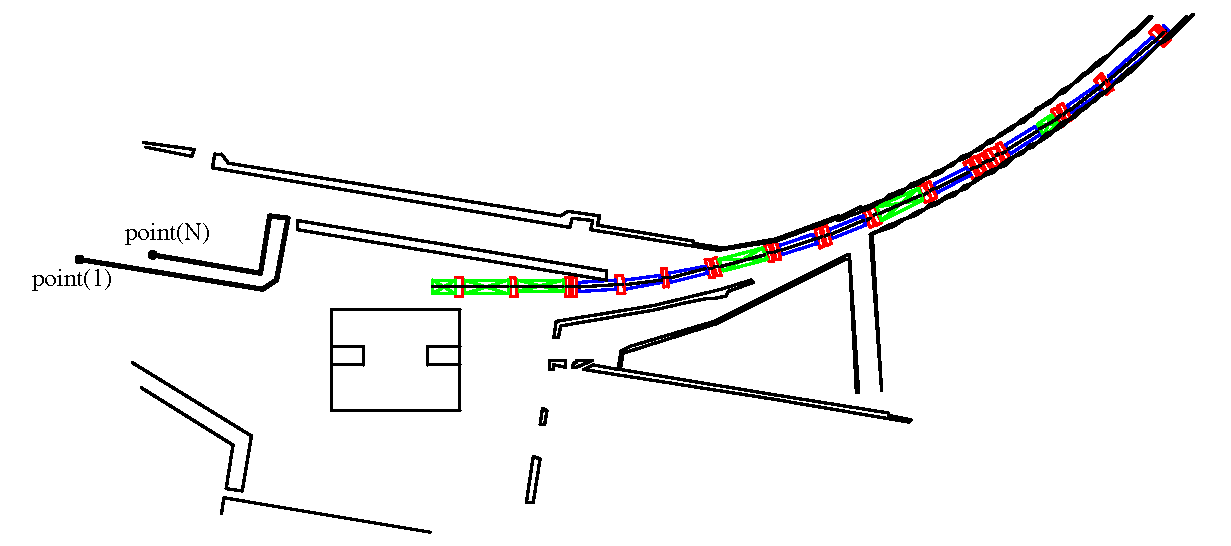
\includegraphics[width=5in]{building-wall.pdf}
  \caption[Floor plot showing the walls of the building]
{Floor plot showing the walls of the building (along with a section
of a recirculation arc). Defining building walls can be useful for
such things as floor plots and designing a machine to fit in an
existing building.}
  \label{f:building.wall}
\end{figure}

A two dimensional outline of the building containing the machine under
simulation may be defined in \tao. This may be useful when drawing
floor plans of the machine (\sref{s:floor.plan}) or to design a
machine to fit within an existing building by optimizing
(\sref{c:opti}) the position of the machine to be within the
building's walls.

The walls of a building are defined by a set of ``sections'' which are
just curves that mark the wall boundaries. One such section is
highlighted in Figure~\ref{f:building.wall} starting at the point
marked ``point(1)'' and ending at the point marked ``point(N)''. Each
section is defined by a set of points which are connected together using
straight lines or circular arcs.

The name of the file containing the building wall definition is given
by the \vn{building_wall_file} variable in the \vn{tao_start} namelist
(\sref{s:init.global}). This file will contain a number of
\vn{building_wall_section} namelists. Each \vn{building_wall_section}
namelist defines a single wall section. The syntax of this namelist is
\begin{example}
  &building_wall_section
    \{constraint = <type>\}
    point(1) = <z1>, <x1>
    point(2) = <z2>, <x2>, \{<r2>\}
    point(3) = <z3>, <x3>, \{<r3>\}
    ... etc ...
    point(N) = <zN>, <xN>, \{<rN>\}
  /
\end{example}
The global coordinate system in \bmad (see the \bmad manual) defines
the $(Z, X)$ plane as being horizontal.  [Note: $(Z, X)$ is used
instead of $(X, Z)$ since $(Z, X, Y)$ forms a right handed coordinate
system.] The points that define a wall section are specified in this
coordinate system.  In the \vn{building_wall_section} namelist, the
$(Z, X)$ position of each point defining a wall section is given along
with an optional radius $r$. If a non-zero radius is given for point
$j$, then the segment between point $j-1$ and $j$ is a circular arc of
the given radius. If no radius is given, or if it is zero, the segment
is a straight line. A radius for the first point, number 1, cannot be
specified since this does not make sense. Additionally, a radius must
be at least half the distance between the two points that define the
end points of the arc.

In general, given two end points and a radius, there are four possible
arcs that can be drawn. The arc chosen follows the following convention:
\begin{enumerate}
\item
The angle subtended by the arc is 180 degrees or less.
\item
If the radius for the arc from $j-1$ to $j$ is positive, the arc
curves in a clockwise manner. If the radius is negative, the arc
curves counterclockwise. This convention mimics the convention used
for \vn{rbend} and \vn{sbend} elements.
\end{enumerate}
To define a wall that is circular, use three points with two 180
degree arcs in between.

When designing a machine to fit within the walls of a building, the
\vn{constraint} variable of the namelist is used to designate whether
the given wall section is on the $+x$ side of the machine or the $-x$
side. Here $x$ is the local reference frame transverse coordinate. See
the write up of the \vn{wall.right_side} and \vn{wall.left_side} constraints in
\sref{s:data.types} for more details. Possible values for
\vn{constraint} are:
\begin{example}
  "right_side"  ! Section is to be used with wall.x+ constraints
  "left_side"   ! Section is to be used with wall.x- constraints
  "none"        ! Default. Section is ignored in any constraint calculation.
\end{example}

Example:
\begin{example}
  &building_wall_section
    constraint = "left_side"   
    point(1) =  23.2837,    8.2842
    point(2) = -10.9703,   13.8712, 107.345
    point(3) = -10.8229,   14.7737
  /
\end{example}
In this example, point 1 is at $(Z, X) = (23.2837, 8.2842)$, the
segment between points 1 and 2 is an arc with a radius of 107.345
meters, and the segment between points 2 and 3 is a straight
line. Also this wall section is to be used when evaluating any
\vn{wall.x+} constraint.

Note: To position a machine in the global coordinate system, the
starting point and starting orientation can be adjusted using
\vn{beginning[...]} statements as explained in the \bmad manual.

%-----------------------------------------------------------------
\section{Initializing Dynamic Aperture}
\index{dynamic aperture}
\label{s:dynamicaperture}

For rings, the dynamic aperture can be calculated if \vn{tao_dynamic_aperture} is defined:

\begin{example}
  &tao_dynamic_aperture
   da_init(ix_uni)%pz = 0, 0.01, ...     ! List of particle energies to use
   da_init(ix_uni)%n_angle = 64          ! Number of angles in scan of each energy
   da_init(ix_uni)%min_angle = 0         ! Starting scan angle.
   da_init(ix_uni)%max_angle = 3.14159   ! Ending scan angle.
   da_init(ix_uni)%n_turn = 100          ! Number of turns a particle must survive
   da_init(ix_uni)%x_init = 1e-3_rp      ! initial estimate for horizontal aperture
   da_init(ix_uni)%y_init = 1e-3_rp      ! initial estimate for vertical aperture
   da_init(ix_uni)%accuracy = 1e-5_rp    ! resolution of bracketed aperture (meters)
  /
\end{example}

where \vn{ix_uni} indicates the universe number. Here \vn{pz} is a list of relative momenta
to calculate the aperture for. If the RF is off, then a new closed orbit will be calculated 
for each of these momenta. 

Optionally parameters \vn{n_angle}, \vn{min_angle}, and \vn{max_angle} can be set to indicate
the angle in the $x-y$ plane to scan about the closed orbit.

By default, the dynamic aperture calculation is off for all universes. To turn it on,
use the \vn{set} command (\sref{s:set}):
\begin{example}
  set universe 1 dynamic_aperture_calc on
\end{example}

If Tao is compiled with the appropriate OpenMP flags, then this calculation will be done in parallel. 

The results can be plotted. See \sref{s:dynamicapertureplot}. 

\clearpage
%-----------------------------------------------------------------
\section{Initializing Plotting}
\index{plotting initializing}
\label{s:init.plot} 

\subsection{Plot Window}
\label{s:plot.page}
\index{initialization!plotting!plot window}

Plotting is defined by an initialization file whose name is defined
by the \vn{tao_start} namelist (\sref{s:init.global}).
The first namelist block in the file has a block
name of \vn{tao_plot_page}. This block sets the size of the plot
window (also called the plot page) and defines the ``regions'' where
plots go. The syntax of this block is:
\index{tao_plot_page}\index{plot_page!n_curve_pts}
\index{plot_page!size}\index{plot_page!border}
\index{plot_page!text_height}\index{plot_page!title}
\index{region!name}\index{region!location}\index{place}
\begin{example}
  &tao_plot_page
    plot_page%plot_display_type        = <string>  ! Display type: 'X' or 'TK'
    plot_page%size                     = <x_size>, <y_size>         ! size in POINTS 
    plot_page%border                   = <x1\(_{\dstyle{b}}\)>, <x2\(_{\dstyle{b}}\)>, <y1\(_{\dstyle{b}}\)>, <y2\(_{\dstyle{b}}\)>, "<units>"
    plot_page%text_height              = <real>   ! height in POINTS. Def = 12
    plot_page%main_title_text_scale    = <real>   ! Relative to text_height. Def = 1.3
    plot_page%graph_title_text_scale   = <real>   ! Relative to text_height. Def = 1.1
    plot_page%axis_number_text_scale   = <real>   ! Relative to text_height. Def = 0.9
    plot_page%axis_label_text_scale    = <real>   ! Relative to text_height. Def = 1.0
    plot_page%legend_text_scale        = <real>   ! Relative to text_height. Def = 0.8
    plot_page%key_table_text_scale     = <real>   ! Relative to text_height. Def = 0.9
    plot_page%floor_plan_shape_scale   = <real>   ! Floor_plan shape size scaling.
    plot_page%lat_layout_shape_scale   = <real>   ! Lat_layout shape size scaling.
    plot_page%title(i)                 = <string>, {<x>, <y>, "<units>", "<justify>"}
    plot_page%n_curve_pts              = <intger> ! Num points used to construct a 
                                                  !   smooth curve. Default = 401
     = <T/F>    ! Used with "show plot" command.
    plot_page%box_plots                = <T/F>    ! For debugging. Default = F.
    include_default_plots              = <T/F>    ! Include default templates? Def = T.
    region(i) = "<region_name>" <x1\(_{\dstyle{r}}\)>, <x2\(_{\dstyle{r}}\)>, <y1\(_{\dstyle{r}}\)>, <y2\(_{\dstyle{r}}\)>  
    place(i)  = "<region_name>", "<template_name>"
    default_plot%...                            ! See below.
    default_graph%...                           ! See below. 
  /
\end{example}

%-----------------------

\begin{figure}[bt]
  \centering
  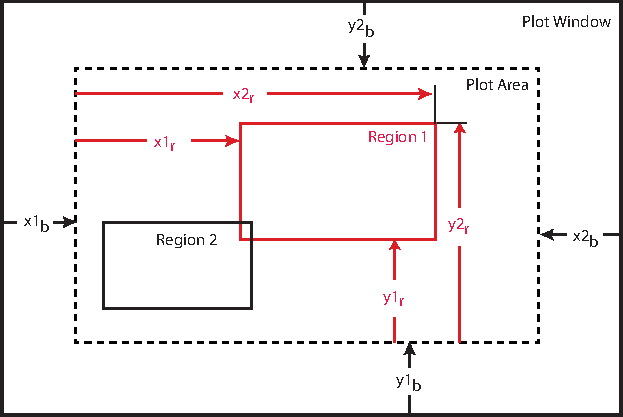
\includegraphics{plot-page.pdf}
  \caption[The plot window.]{The plot window has a boarder whose position is determined by 
the \vn{plot_page\%border} parameter in the tao_plot_page namelist.  Plots are placed
in ``\vn{regions}'' whose location is determined by the setting of the \vn{region(i)} parameters in
the same namelist. Regions may overlap.} 
  \label{f:plot.page}
\end{figure}

%-----------------------

For example:
\begin{example}
  &tao_plot_page
    plot_page%plot_display_type = "X"        ! X11 window.  "TK" is alternative.
    plot_page%size        = 700, 800         ! Points
    plot_page%border      = 0, 0, 0, 50, "POINTS"  
    plot_page%text_height = 12.0
    plot_page%title(1)    = "CESR Lattice", 0.5, 0.996, "%PAGE", "CC"
    region(1) = "top"    0.0, 1.0, 0.5, 1.0
    region(2) = "bottom" 0.0, 1.0, 0.0, 0.5
    place(1)  = "top",    "orbit"
    place(2)  = "bottom", "phase"
    default_plot%x%min = 100
    default_plot%x%max = 200
  /
\end{example}

\vn{plot_page%size} sets the horizontal and vertical size of the plot
window in \vn{points} units (72 points = 1 inch. Roughly 1 point = 1
pixel). 

\vn{plot_page%text_height} sets the overall height of the text that is
drawn. Relative to this, various parameters can be used to scale
individual types of text:
\begin{example}
  plot_page%main_title_text_scale  = 1.3 ! Main title height. 
  plot_page%graph_title_text_scale = 1.1 ! Graph title height.
  plot_page%axis_number_text_scale = 0.9 ! Axis number height
  plot_page%axis_label_text_scale  = 1.0 ! Axis label height.
  plot_page%key_table_text_scale   = 0.8 ! Key Table text (\sref{s:key.table}).
  plot_page%legend_text_scale      = 0.9 ! Lat Layout or floor plan text.
\end{example}
The default values for these scales are given above.

The \vn{plot_page%plot_display_type} component sets the type of plot display
window used. possibilities are:
\begin{example}
  "X"      X11 window
  "TK"     tk window
  "QT"     Available only when using PLPLOT (and not the default PGPLOT)
\end{example}
Note: The environmental variable \vn{ACC_PLOT_DISPLAY_TYPE} sets the default display
type. You can set this variable in your login file to avoid having to setup a \tao
init file to set this.

\vn{plot_page%border} sets a border around the edges of the window. As shown in
Figure~\ref{f:plot.page} x1$_{\dstyle{b}}$, x2$_{\dstyle{b}}$ are the right and left border widths
and y1$_{\dstyle{b}}$ and y2$_{\dstyle{b}}$ are the bottom and top border widths respectively.  The
rectangle within this border is called the plot area.

\vn{plot_page%title(i)} set the page title. There are two title areas (i = 1,2). If only the title
string is given then the other variables are set to the defaults \vn{x} = 0.5, \vn{y} = 0.995,
\vn{justify} = "CC" and \vn{units} = "\vn{%PAGE}". See the quickplot documentation for the
\vn{justify} variable syntax.

The plot area is divided up into rectangular regions where plots may be placed (what defines a plot
is discussed below).  \vn{region(i)} in the \vn{tao_plot_page} namelist is an array of five elements
that defines the i\Th region. The first element of this array is the name of the region. This name
may not contain a dot ``.''.  The last four elements of the \vn{retion(i)} array, x1$_{\dstyle{r}}$,
x2$_{\dstyle{r}}$, y1$_{\dstyle{r}}$ and y2$_{\dstyle{r}}$ define the location of the region as
illustrated in Figure~\ref{f:plot.page}.  x1$_{\dstyle{r}}$ and x2$_{\dstyle{r}}$ are normalized to
the width of the plot area and y1$_{\dstyle{r}}$ and y2$_{\dstyle{r}}$ are normalized to the height
of the plot area. That is, these four number should be in the range $[0, 1]$.  Regions may overlap
any one can define as many regions as one likes.

Besides the regions that the user sets up in the \vn{tao_plot_page} namelist, \tao defines a number
of default regions whose names begin with the letter '\vn{r}'. Use the \vn{show plot} command
(\sref{s:plot}) to view a list of these plots.

When \vn{plot_page%delete_overlapping_plots} is True (the default), Placing a plot (using
the \vn{place} command \sref{s:place}) causes any existing plots that overlap the
placed plot to become invisible. 

The \vn{plot_page%n_curve_pts} sets the default number of points to use for drawing ``smooth''
curves. Default is 401. This default may be overridden by setting the \vn{plot%n_curve_pts}
component of a plot (\sref{s:template}).

\vn{place(i)} determines the initial placement of plots.

\vn{default_plot} sets the defaults for any \vn{plot}s
defined in the \vn{tao_template_plot} namelists
(\sref{s:template}). Similarly, \vn{default_graph} sets defaults for the
\vn{graph} structure defined in the \vn{tao_template_graph} namelist
(\sref{s:template}). In the example above, the default x-axis min and
max are set to 100 and 200 respectively.

If \vn{include_default_plots} is set to \vn{False}, the collection of default template
plots (\sref{s:template}) that \tao uses by default are not used along with the template
plots defined in the plotting file.

%-----------------------------------------------------------------
\subsection{Plot Templates}
\label{s:template}
\index{plot templates}

As shown in Figure~\ref{f:plot}, a ``plot'' is made up of a collection
of ``graphs'' and a graph consists of axes plus a set of ``curves''.
In the \vn{tao_plot.init} file there needs to be defined a set of
``template plots''. A template plot specifies the layout of a plot:
How the graphs are placed within a plot, what curves are associated
with what graphs, etc. When running \tao, the information in a
template plot may then be transferred to a region using the \vn{place}
command and this will produce a visible plot.

Template plots are defined using namelists with a name of
\vn{tao_template_graph}. The general syntax is:
\index{tao_template_plot}
\index{plot!name}
\index{plot!x}
\index{plot!x_axis_type}
\index{plot!n_graph}
\index{plot!autoscale_gang_x}
\index{plot!autoscale_gang_y}
\index{plot!autoscale_x}
\index{plot!autoscale_y}
\begin{example}
  &tao_template_plot
    plot%name        = "<plot_name>"
    plot%x           = <qp_axis_struct>
    plot%x_axis_type = "<x_axis_type>"   ! "index", "ele_index" "s", "lat", or "var". 
                                         ! Default is "index".
    plot%n_graph     = <n_graphs>
    plot%autoscale_gang_x = <logical>    ! Default: True.
    plot%autoscale_gang_y = <logical>    ! Default: True.
    plot%autoscale_x = <logical>         ! Default: False.
    plot%autoscale_y = <logical>         ! Default: False.
    plot%n_curve_pts = <integer>         ! Used to override plot_page%n_curve_pts.
    default_graph%...                    ! See below
  /
\end{example}
For example:
\begin{example}
  &tao_template_plot
    plot%name                = "orbit"
    plot%x%min               =   0
    plot%x%max               = 100
    plot%x%major_div_nominal = 10
    plot%x%label             = "Index"
    plot%n_graph             = 2
    default_graph%y%max      = 10
  /
\end{example}

\vn{default_graph} sets defaults for the \vn{graph} structure defined
in the \vn{tao_template_graph} namelist (\sref{s:template}). This
overrides \vn{default_graph} settings made in the
\vn{tao_template_plot} namelist (\sref{s:init.plot}) but only for
graphs associated with the \vn{tao_template_plot} the
\vn{default_graph} is defined in.

\vn{plot%x} sets the properties of the horizontal axis. For more
information see the \vn{Quick Plot} documentation on the
\vn{qp_axis_struct} in the Bmad manual. The major components are
\index{qp_axis_struct!min}
\index{qp_axis_struct!max}
\index{qp_axis_struct!major_div_nominal}
\index{qp_axis_struct!major_div}
\index{qp_axis_struct!minor_div}
\index{qp_axis_struct!label}
\begin{example}
  min        ! Left edge value.
  max        ! Right edge value.
  major_div  ! Number of major divisions. 
             !  Number of major tick marks is one less.
  major_div_nominal ! Nominal number of major divisions
  minor_div  ! Number of minor divisions. 0 = auto choose.
  label      ! Axis label.
\end{example}
If \vn{min} and \vn{max} are absent, then \tao will autoscale the
axis.  If it is desired to have differing scales for different graphs,
the \vn{graph%x} component can be used (see below).

Both \vn{major_div} and \vn{major_div_nominal} set the number of major
divisions in the plot. The difference between the two is that with
\vn{major_div} the number of major divisions is fixed at the set value
and with \vn{major_div_nominal} the number of major divisions can vary
from the set value when \tao scales a graph. If
\vn{major_div_nominal} is set, this will override any setting of
\vn{major_div}. If neither \vn{major_div} nor \vn{major_div_nominal}
is set, a value will be chosen for \vn{major_div_nominal} by \tao. If
you are unsure which to set, it is recommended that
\vn{major_div_nominal} be used.

Plots with \vn{plot%autoscale_x} and/or \vn{plot%autoscale_y}
logicals, set to true will automatically rescale after any
calculation. The \vn{plot%autoscale_gang_x} and
\vn{plot%autoscale_gang_y} components set how the \vn{x_scale}
(\sref{s:x.scale}) and \vn{scale} (\sref{s:scale}) commands behave
when autoscaling entire plots. See these individual commands for more
details.

\vn{plot%name} is the name that is used with \tao commands to identify
the plot. It is important that this name not contain any blank spaces since
\tao uses this fact in parsing the command line. 

\vn{plot%x_axis_type} sets what is plotted along the
\vn{x_axis}. Possibilities are:
\index{index}
\index{ele_index}
\index{s}
\begin{example}
    "index"      ! Data Index
    "ele_index"  ! Element lattice number index
    "s"          ! Longitudinal position in the lattice.
    "data"       ! From a data array
    "lat"        ! Lattice variable. See \sref{s:plot.var}.
    "var"        ! Tao variable value. See \sref{s:plot.var}.

\end{example}
The \vn{ele_index} switch is used when plotting data arrays. In this
case the \vn{index} switch refers to the index of the data array and
\vn{ele_index} refers to the index of the lattice element that the
datum was evaluated at.

\vn{n_graph} sets the number of graphs associated with the plot and
each one needs a \vn{tao_template_graph} namelist to define it. These
namelists should be placed directly after their respective
\vn{tao_template_graph} namelists. The general format of the
\vn{tao_template_graph} namelist is:
\index{tao_template_graph}\index{graph!y}\index{curve!name}
\index{graph_index}\index{graph}\index{graph!name}\index{curve}
\index{graph!type}\index{graph!box}\index{graph!title}\index{graph!margin}
\index{graph!y2}\index{graph!n_curve}\index{graph!clip}\index{graph!component}
\index{graph!symbol_size_scale}
\index{graph!floor_plan_rotation}
\index{graph!floor_plan_view}
\index{curve!data_type}\index{curve!data_source}
\index{curve!x_axis_units_factor}\index{curve!y_axis_units_factor}
\index{curve!use_y2}\index{curve!line}\index{curve!ele_ref_name}
\index{curve!draw_line}\index{curve!draw_symbols}\index{curve!ix_universe}
\index{curve!symbol}\index{curve!symbol_every}\index{curve!convert}
\index{curve!ix_bunch}\index{curve!ix_ele_ref}\index{curve!data_type_x}
\begin{example}
  &tao_template_graph
    graph_index             = <integer>
    graph%name              = "<string>"       ! Default is  "g<n>" <n> = graph_index. 
    graph%type              = "<string>"       ! "data", "floor_plan", etc.
    graph%box               = <ix>, <iy>, <ix_tot>, <iy_tot>
    graph%title             = "<string>"       ! Title above the graph.
    graph%margin            =  <ix1>, <ix2>, <iy1>, <iy2>, "<Units>"
    graph%scale_margin      =  <ix1>, <ix2>, <iy1>, <iy2>, "<Units>"
    graph%x                 = <qp_axis_struct> ! Horizontal axis.
    graph%y                 = <qp_axis_struct> ! Left axis.
    graph%y2                = <qp_axis_struct> ! Right axis.
    graph%clip              = <logical>        ! Clip curves at boundary? Default = T
    graph%draw_axes         = <logical>        ! Default = T
    graph%draw_grid         = <logical>        ! Default = T
    graph%allow_wrap_around = <logical>        ! Wrap curves around lattice ends?
    graph%component         = "<string>"       ! Eg: "model - design"
    graph%symbol_size_scale      = <real>      ! Phase_space plots symbol scale factor
    graph%correct_xy_distortion  = <logical>   ! For Floor Plan plots: Default = F
    graph%ix_universe            = <integer>   ! Default = -1 => Use default universe
    graph%floor_plan_rotation    = <real>      ! Rotation of floor plan plot: 1.0 -> 360 deg. 
    graph%floor_plan_view        = <string>    ! View plane for floor plan plot. default = 'zx'
    graph%floor_plan_orbit_scale = <real>      ! Scale for drawing orbits. Default: 0 -> Do not draw.
    graph%floor_plan_orbit_color = <string>    ! Color of orbit. Default = 'RED'
    graph%floor_plan_size_is_absolute = <logical>     ! Shape sizes scaled to absolute dimensions?
    graph%floor_plan_draw_only_first_pass = <logical> ! Draw only first pass with multipass elements?
    graph%draw_only_good_user_data_or_vars     ! Veto data or variables with good_user = F?
                                 = <logical>   !   Default = T.
    graph%x_axis_scale_factor    = <factor>    ! Scale the x-axis by this.
    graph%n_curve                = <integer>   ! number of curves
    curve(i)%name                = "<string>"  ! Default is "c<i>", <i> = curve num.
    curve(i)%data_source         = "<string>"  ! Source for the data curve points
    curve(i)%data_type_x         = "<string>"  ! Used with plot%x_axis_type = "data" or "var".
    curve(i)%data_type           = "<string>"  ! Default = plot%name.graph%name
    curve(i)%component           = "<string>"  ! Eg: "model - design". Overrides graph%component.
    curve(i)%data_index          = "<string>"  ! Index number for data points.
    curve(i)%legend_text         = "<string>"  ! Text for curve legend. 
                                               !   Default is the data_type.
    curve(i)%y_axis_scale_factor = <factor>    ! Scale the y-axis by this.
    curve(i)%use_y2              = <logical>   ! Use left-axis scale?
    curve(i)%draw_line           = <logical>   ! Connect data with lines?
    curve(i)%draw_symbols        = <logical>   ! Draw data symbols?
    curve(i)%draw_symbol_index   = <logical>   ! Print index number next to the data symbol?
    curve(i)%ix_universe         = <integer>   ! Default = -1 => Use graph%ix_universe.
    curve(i)%ix_branch           = <integer>   ! Default = 0  => Use main lattice.  
    curve(i)%ix_bunch            = <integer>   ! Bunch index. Default = 0 (all bunches).
    curve(i)%line        = <qp_line_struct>    ! Line spec (color, width, etc.)
    curve(i)%symbol      = <qp_symbol_struct>  ! Symbol spec (color size, etc.)
    curve(i)%symbol_every     = <integer>      ! Plot symbol every # datums
    curve(i)%ele_ref_name     = "<string>"     ! Name of reference element.
    curve(i)%ix_ele_ref       = <integer>      ! Index number of reference element.
    curve(i)%smooth_line_calc = <Logical>      ! Calc data between symbol points? 
    curve(i)%units            = "<string>"     ! Data units
  /
\end{example}
For example:
\begin{example}
  &tao_template_graph
    graph_index               = 1
    graph%name                = "x"
    graph%type                = "data"
    graph%box                 = 1, 1, 1, 2
    graph%title               = "Horizontal Orbit (mm)"
    graph%margin              =  60, 200, 30, 30, "POINTS"
    graph%y%label             = "X"
    graph%y%max               =  4
    graph%y%min               = -4
    graph%y%major_div_nominal = 4
    graph%n_curve             = 1
    graph%component           = "model - design"
    curve(1)%data_source      = "data"
    curve(1)%data_type        = "orbit.x"
    curve(1)%units_factor     = 1000
    curve(1)%use_y2           = F
  /
\end{example}

\vn{graph%title} is the string just above the graph. The full string will also include information
about what is being plotted and the horizontal axis type. To fully suppress the title leave it
blank.

If there are multiple curves drawn with a graph then a curve legend showing what lines are
associated with what data will be drawn. The default is to draw this legend in the upper left hand
corner of the graph. By default, the \vn{data_type} of each curve will be used as the text for that
curve's line in the legend.  This default can be changed by setting a curve's \vn{curve%legend_tex}.

\vn{graph%name} and \vn{curve%name} define names to be used with commands. The default names are
just the letter \vn{g} or \vn{c} with the index of the graph or curve. Thus, in the example above,
the name of the curve defaults to \vn{c1} and it would be referred to as \vn{orbit.x.c1}.  It is
important that these names do not contain any blank spaces since \tao uses this fact in parsing the
command line.

\vn{graph%box} sets the layout of the box which the \vn{graph} is placed in. For a definition of
what a box is see the Quick Plot documentation in the \bmad reference manual. In the above example
the graph divides the region into two vertically stacked boxes and places itself into the bottom
one.

\vn{graph%allow_wrap_around} sets if, for a lattice with closed geometry, the curves contained in
the graph are ``wrapped'' around the ends of the lattice. The default is \vn{True}.

\vn{graph%margin} sets the margin between the \vn{graph} and the \vn{box}
it is drawn in.

\vn{graph%scale_margin} is used to set the minimum space between what is being drawn and the edges
of the \vn{graph} when a \vn{scale}, \vn{x_scale}, or a \vn{xy_scale} command is issued. Normally
this is zero but is useful for \vn{floor plan} drawings.

\vn{graph%type} is the type of graph. \tao knows about the
following types:
\index{data}\index{lat_layout}\index{key_table}\index{phase_space}
\index{floor_plan}\index{beam_chamber_wall}
\begin{example}
  "data"               ! Data and/or variable plots (default) (\sref{s:plot.data}).
  "floor_plan"         ! A 2-dimensional birds-eye view of the machine (\sref{s:floor.plan}).
  "histogram"          ! Histogram of plot (\sref{s:histogram}).
  "key_table"          ! Key binding table for single mode (\sref{s:key.table}).
  "lat_layout"         ! Schematic showing placement of the lattice elements (\sref{s:lat.layout}).
  "phase_space"        ! Phase space plots (\sref{s:phase.space}).
\end{example}

With \vn{graph%type} set to \vn{"beam_chamber_wall"} (\sref{s:beam.wall.draw}), the beam chamber
wall is drawn if it has been defined in the \bmad lattice file.

With \vn{graph%type} set to \vn{"data"} (\sref{s:plot.data}), data such as orbits and/or variable
values such as quadrupole strengths are plotted. Here ``data'' can be data from a defined data
structure (\sref{c:data}) or computed directly from the lattice, beam tracking, etc. A \vn{"data"}
graph type will contain a number of \vn{curves} and multiple data and variable curves can be drawn
in one graph.

With \vn{graph%type} set to \vn{floor_plan} (\sref{s:floor.plan}), the two dimensional layout of the
machine is drawn.

With \vn{graph%type} set to \vn{histogram} (\sref{s:histogram}), such things such as beam densities
can be histogrammed.

With \vn{graph%type} set to \vn{"key_table"} (\sref{s:key.table}), the key bindings for use in
single mode (\sref{s:key.bind}) are displayed.  Note: The \vn{"key_table"} graph type does not have
any associated \vn{curve}s.

With \vn{graph%type} set to \vn{lat_layout} (\sref{s:lat.layout}), the elements of the lattice are
symbolical drawn in a one dimensional line as a function of the longitudinal distance along the
machine centerline.

With \vn{graph%type} set to \vn{phase_space} (\sref{s:phase.space}), phase space plots are produced.

%-----------------------------------------------------------------
\subsection{Data and Variable plotting}
\label{s:plot.data}

A \vn{graph} (\sref{s:template}), with \vn{graph%type} equal to \vn{"data"}, is used to draw
``data'' such as orbits and/or variable values such as quadrupole strengths. A data \vn{graph} will
have a number of associated \vn{curve}s with each curve defining a particular data type to plot.

The data values will depend upon where the data comes from. This is determined, in part, by the
setting of \vn{graph%component} and \vn{curve%component}. \vn{graph%component} and
\vn{curve%component} may be one of:
\index{model}\index{design}\index{base}\index{meas}\index{ref}
\begin{example}
  "model"             ! model values. Default.
  "design"            ! design values.
  "base"              ! Base values
  "meas"              ! data values.
  "ref"               ! reference data values.
  "beam_chamber_wall" ! Beam chamber wall
\end{example}
Additionally, \vn{graph%component} may be set to plot a linear combination of the above. For
example:
\begin{example}
  graph%component = "model - design"
\end{example}
This will plot the difference between the \vn{model} and \vn{design} values.

If \vn{curve%component} is set, it will override \vn{graph%component}. If \vn{graph%component} is
not set in the initialization file, and if there are curves of the graph that have not been set,
\vn{graph%component} will be given a default setting of \vn{model}.

\index{data}\index{var}\index{calculation}
\index{curve!data_source}
The \vn{curve} structure is used to define the data that is plotted in each graph.
\vn{curve%data_source} is the type of information for the source of the data points.
\vn{curve%data_source} must be one of:
\begin{example}
  "data"              ! A d1_data array is the source of the curve points.
  "var"               ! A v1_var array is the source of the curve points.
  "lat" (Default)     ! The curve points are computed directly from the lattice.
  "beam"              ! The curve points are computed tracking a beam of particles.
  "multi_turn_orbit"  ! Computation is from multi-turn tracking. 
\end{example}
The default for \vn{curve%data_source} is \vn{"lat"}. With \vn{curve%data_source} set to \vn{data},
the values of the curve points come from the \vn{d1_data} array structure named by
\vn{curve%data_type}. Thus in the above example the curve point values are obtained from
\vn{orbit.x} data. To be valid the data structure named by \vn{curve%data_type} must be set up in an
initialization file. If not given, the default \vn{curve%data_type} is
\begin{example}
  <plot%name>.<graph%name>
\end{example}
If \vn{curve%data_source} is set to \vn{var}, the values of the curve points come from a \vn{v1_var}
array structure. If it is set to \vn{lat} the curve data points are calculated from the lattice
without regard to any data structures. \vn{curve%data_source} can be set to \vn{beam} when tracking
beams of particles. In this case, the curve points are calculated from the tracking. With \vn{beam},
the particular bunch that the data is extracted from can be specified via \vn{curve%ix_bunch}. The
default is \vn{0} which combines all the bunches of the beam for the calculation.

Example: With \vn{curve%data_type} set to \vn{beta.x}, the setting of \vn{curve%data_source} to
\vn{lat} gives the beta as calculated from the lattice and \vn{beam} gives the beta as calculated
from the shape of the beam.

\vn{curve%draw_symbols} determines whether a symbol is drawn at the data points. The size, shape and
color of the symbols is determined by \vn{curve%symbol}. A given symbol point that is drawn has
three numbers attached to it: The $(x, y)$ position on the graph and an index number to help
identify it. The index number of a particular symbol is the index of the datum or variable
corresponding the symbol in the \vn{d1_data} or \vn{v1_var} array. These three numbers can be
printed using the \vn{show curve -symbol} command (\sref{s:show}).  \vn{curve%draw_symbol_index}
determines whether the index number is printed besides the symbol. Use the \vn{set curve} command
(\sref{s:set}) to toggle the drawing of symbols. The default value for \vn{curve%draw_symbol} is
False if \vn{plot%x_axis_type} is \vn{"s"} and True otherwise. The
default\vn{curve%draw_symbol_index} is always False.

\vn{curve%draw_line} determines whether a curve is drawn through the data point symbols. The
thickness, style (solid, dashed, etc.), and color of the line can be controlled by setting
\vn{curve%line}. If \vn{plot%x_axis_type} is \vn{"s"}, and \vn{graph%component} does not contain
\vn{"meas"} or \vn{"ref"}, \tao will attempt to calculate intermediate values in order to draw a
smooth, accurate curve is drawn. Occasionally, this process is too slow or not desired for other
reasons so setting \vn{curve%smooth_line_calc} to False will prevent this calculation and the curve
will be drawn as a series of lines connecting the symbols. The default of
\vn{curve%smooth_line_calc} is True. Use the \vn{set curve} command (\sref{s:set}) to toggle the
drawing of lines. Alternatively, the \vn{-disable_smooth_line_calc} switch can be used on the
command line (\sref{s:command.line}) or the global variable \vn{global%disable_smooth_line_calc} can
be set in the \tao initialization file (\sref{s:globals}).

The \vn{graph%draw_only_good_user_data_or_vars} switch determines whether datums
(\sref{s:init.data}) or variables (\sref{s:init.var}) with a \vn{good_user} component set to
\vn{False} are drawn. The default is to not draw them which means that data or variables not used in
an optimization are not drawn.

A graph has two vertical axes. The one on the left is called \vn{"y"} and the one on the right is
called \vn{"y2"}. For example, \vn{graph%y%label} sets the axis label for the \vn{y} axis and
\vn{graph%y2%label} sets the axis label for the \vn{y2} axis. Normally there is only one vertical
scale for a graph and this is associated with the \vn{y} axis. However, if any curve of a given
graph has \vn{curve%use_y2} set to \vn{True} then the \vn{y2} axis will have an independent second
scale. In this case, the \vn{y2} axis numbers will be drawn. Notice that simply giving the \vn{y2}
axis a label does {\em not} make the \vn{y2} axis scale independent of the \vn{y} axis scale.

Typically, a graph's horizontal scale is set by the \vn{plot%x} component. If it is desired to have
differing scales for different graphs, the \vn{graph%x} component can be used.

%-----------------------------------------------------------------
\subsection{Graphing a Data Slice}\index{plot!data slice}
\label{s:graph.data.slice}

The standard data graph, as presented in the previous subsection,
plots data from a given \vn{d1_data} array. It is also possible to
graph data that has been ``sliced'' in other ways. For example,
suppose a number of universes have been established, with each
universe representing the same machine but with different steerings
powered. If in each universe an \vn{orbit} \vn{d2_data} structure has
been defined, an example of a data slice is the collection of
points (x, y) where:
\begin{example}
  (x, y) = (<n>@orbit.x[23], <n>@orbit.y[23]),   <n> = 1, ..., n_universe
\end{example}
When defining a template for graphing a data slice, the
plot%x_axis_type is set to \vn{"data"}, and the \vn{graph%type} must
be set to \vn{"data"}, the \vn{curve(:)%data_source} must be set to
\vn{"data"} and the \vn{curve(:)%data_type_x} and
\vn{curve%data_type} are used to define the x and y axes respectively.
In the strings given by \vn{<curve%data_type_x} or
\vn{<curve%data_type}, all substrings that look like \vn{\#ref} are
eliminated and the string given by \vn{curve%ele_ref_name} is
substituted in its place.  Similarly, a \vn{\#comp} string is used as a
place holder for the \vn{graph%component} Example:
\begin{example}
  &tao_template_plot
    plot%name = "at_bpm"
    plot%x%label = "x"
    plot%x_axis_type = "data"
    plot%n_graph = 1
  /

  &tao_template_graph
    graph_index = 1
    graph%title = "Orbit at BPM"
    graph%y%label = "y"
    graph%component = "meas - ref"
    graph%type = "data"
    graph%n_curve = 1
    graph%x_axis_scale_factor = 1000
    curve(1)%data_source = "data"
    curve(1)%data_type_x = "[2:57]@orbit.x[#ref]|#comp"
    curve(1)%data_type   = "[2:57]@orbit.y[#ref]|#comp"
    curve(1)%data_index  = "[2:57]@orbit.y[#ref]|ix_uni"
    curve(1)%y_axis_scale_factor = 1000
    curve(1)%ele_ref_name = "23"
    curve(1)%draw_line = F
  /
\end{example}
In this example, \vn{curve(1)%data_type_x} expands to
\vn{"[2:57]@orbit.x[23]|meas-ref"}. That is, the \vn{meas - ref}
values of \vn{orbit.x[23]} from universes 2 through 57 is used for the
x-axis.  Similarly, \vn{orbit.y[23]} is used for the y-axis. The
\vn{set} command (\sref{s:set}) can be used to change
\vn{curve%ele_ref_name} and \vn{graph%component} strings. 

\vn{curve%data_index} sets the index number for the symbol points
(\sref{s:template}). In the above example, \vn{curve%data_index} is
set to \vn{"[2:57]@orbit.y[\#ref]|ix_uni"}. The \vn{|ix_uni} component
will result in the symbol index number being the universe number.
Additionally, the component \vn{|ix_d1} can be used to specify the
index in the \vn{d1_data} array, and the component \vn{|ix_ele} can be
used to specify the lattice element index. Setting the symbol index
number is important when \vn{curve%draw_symbol_index} is set to True
so that the symbol index is drawn with the curve. Additionally, the
command \vn{show curve -symbol} (\sref{s:show}) will print the symbol
index number along with the $(x, y)$ coordinates of the symbols.

Arithmetic expressions (\sref{s:arithmetic.exp}) may be mixed with
explicit datum components in the specification of
\vn{curve(:)%data_type_x} and \vn{curve(:)%data_type}. Example:
\begin{example}
  curve(1)%data_type_x = "[#ref]@orbit.x|model"
  curve(1)%data_type   = "[#ref]@orbit.x|meas-ref"
  curve(1)%ele_ref_name = "3"
\end{example}
The plots the \vn{model} values of \vn{orbit.x} verses \vn{meas - ref}
of \vn{orbit.x} for the data in universe 3. Note: Whenever explicit
components are specified, the \vn{graph%component} settings are ignored for
that expression.

%-----------------------------------------------------------------
\subsection{Plotting With a Variable Parameter on the X-Axis}
\index{plot!plotting as a function of a variable}
\label{s:plot.var}

Data can be plotted as a function of a lattice parameter by setting
\vn{plot%x_axis_type} to \vn{"lat"} (for lattice variables) or
\vn{"var"} (for \tao variables) and setting \vn{curve(:)%data_type_x}
to the name of the variable. In this case, the \vn{curve(:)%data_type}
must evaluate to a single number.

Example:
\begin{example}
  &tao_template_plot
    plot%x_axis_type = "lat"
    plot%n_curve_pts = 50
    ...
  /

  &tao_template_graph
    ...
    curve(1)%data_type_x = "beam_start[x]"  ! X-axis values.
    curve(1)%data_type   = "orbit.x[10]"    ! Y-axis values.
    ...
  /
\end{example}
Here the number of curve points has been set to 50 to reduce the evaluation overhead.

Note: \tao treats the \vn{design} and \vn{base} lattices as static so
that varying a variable will not affect these lattices. Thus,
constructing a plot with \vn{graph%component} set to, for example,
\vn{"model - design"} will {\em not} produce a plot that is the
difference between varying a variable in both \vn{model} and
\vn{design} lattices. In the case where such a plot is desired, a
second universe needs to be established. In this case, one would set
\vn{curve(:)%data_type} to something like
\begin{example}
    curve(1)%data_type   = "1@orbit.x[10] - 2@orbit.x[10]"    
\end{example}
where the universe \#2 \vn{model} lattice would be setup to be equal
to the universe \#1 \vn{design} lattice.

%-----------------------------------------------------------------
\subsection{Drawing a Lattice Layout}
\index{lattice layout}
\label{s:lat.layout}

\begin{figure}
  \centering
  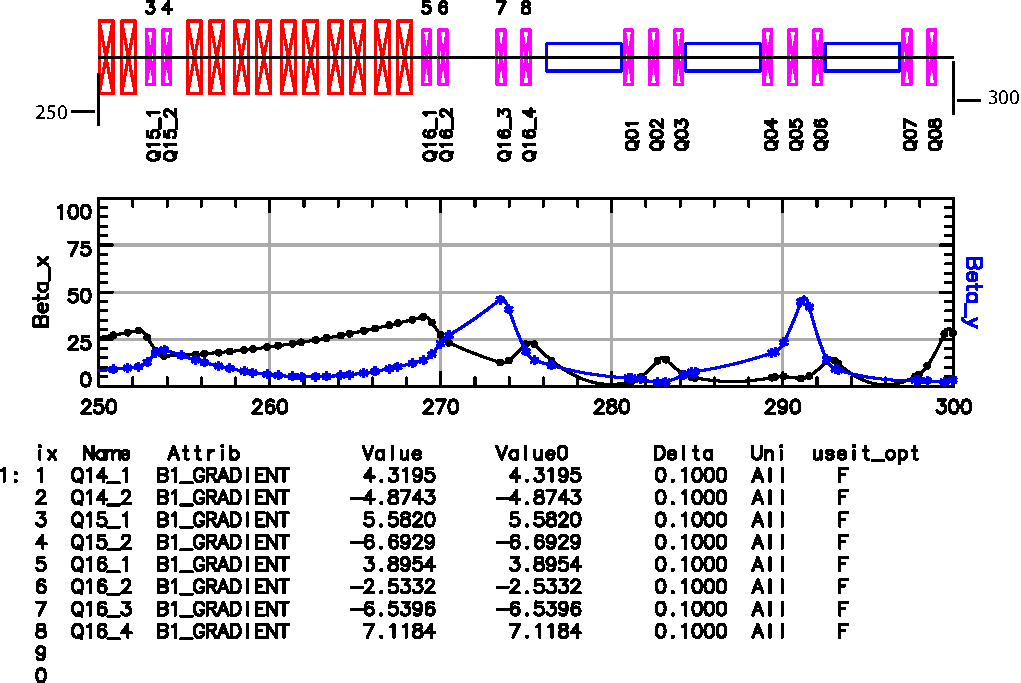
\includegraphics[width=5in]{layout-graph-table.pdf}
  \caption[Example lattice layout and data plots]
{A lattice layout plot (top) above a data plot (middle) 
which in turn is above a key table plot (bottom). The points on the
curves in the data plot mark the edges of the elements displayed in
the lattice layout. Elements that have attributes that are varied as
shown in the key table have the corresponding key table number printed
above the element's glyph in the lattice layout.}
  \label{f:layout.table}
\end{figure}

A lattice layout plot draws the lattice
along a straight line with colored rectangles representing the various elements.
An example is shown in Figure~\ref{f:layout.table}.
The \vn{tao_template_plot} needed to define a lattice layout looks like:
\index{tao_template_plot}\index{plot!name}
\index{plot!x!min}\index{plot!x!max}\index{plot!n_graph}
\index{tao_template_graph}\index{graph_index}\index{graph!name}
\index{graph!type}\index{graph!title}\index{graph!box}
\index{graph!ix_universe}\index{graph!margin}\index{graph!n_curve}
\begin{example}
  &tao_template_plot
    plot%name        = "<plot_name>"
    plot%x%min       = <real>  
    plot%x%max       = <real>  
    plot%n_graph     = <integer>
    plot%x_axis_type = "s"
  /
  &tao_template_graph
    graph_index       = <integer>
    graph%name        = <name>
    graph%type        = "lat_layout"
    graph%title       = "Layout Title"
    plot%box          = <ix>, <iy>, <ix_tot>, <iy_tot>
    graph%ix_universe = <integer> ! -1 => use current default universe
    graph%ix_branch   = <integer> !  0 => use main lattice.
    graph%margin      = <ix1>, <ix2>, <iy1>, <iy2>, "<Units>"
    graph%y%min       = <real>    ! Default: -100
    graph%y%max       = <real>    ! Default:  100
  /
\end{example}
Example:
\begin{example}
  &tao_template_plot
    plot%name        = "layout"
    plot%x%min       =   0
    plot%x%max       = 100
    plot%n_graph     = 1
    plot%x_axis_type = "s"
  /

  &tao_template_graph
    graph_index       = 1
    graph%name        = "u1"
    graph%type        = "lat_layout"
    graph%box         = 1, 1, 1, 1
    graph%ix_universe = 1
    graph%margin      = 0.12, 0.12, 0.30, 0.06, "%BOX"
  /
\end{example}

Which elements are drawn is under user control and is defined 
using an \vn{lat_layout_drawing} namelist. See Section~\sref{s:layout.and.floor}
for more details.

The longitudinal distance markers at either end of the lattice layout can be 
suppressed by setting
\begin{example}
  graph%x%draw_numbers = F
\end{example}

%-----------------------------------------------------------------
\subsection{Drawing a Floor Plan}
\index{floor plan drawing}
\label{s:floor.plan}

\begin{figure}
  \centering
  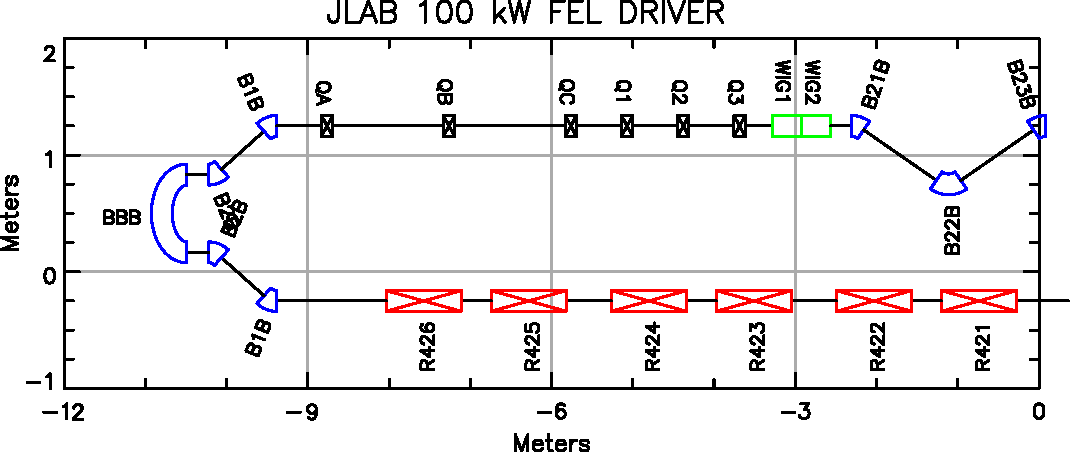
\includegraphics[width=5in]{floor-plan.pdf}
  \caption{Example Floor Plan drawing.}
  \label{f:floor.plan}
\end{figure}

A \vn{floor plan} drawing gives a display of the machine projected
onto the horizontal plane.  An example is shown in
Figure~\ref{f:floor.plan}. Like a \vn{Lattice Layout}
(\sref{s:lat.layout}), Elements are represented by colored rectangles
and which elements are drawn is determined by an
\vn{floor_plan_drawing} namelist (see~\sref{s:layout.and.floor}).

The placement of an element in the drawing is determined by the
element's coordinates in \vn{global reference system}.  See the Bmad
manual for more information on the \vn{global reference system}.  In
the \vn{global reference system}, the $(Z, X)$ plane is the horizontal
plane. 

What plane a floor plan is projected onto is determined by the setting
of the \vn{graph%floor_plan_view} switch. This switch is a two
character string.  Each character is either 'x', 'y', or 'z' and the
characters must not be both the same. Default is 'zx'. The first
character determines which global coordinate are mapped to the
horizontal axis of the graph and the second character determines which
global coordinate is mapped to the vertical axis of the graph. There
are six possible two character combinations. The default 'zx' setting
represents looking at the horizontal plane from above. A setting of
'xz' represents looking at the horizontal plane from below. Etc.

An overall rotation of the floor plan can be controlled by setting
\vn{graph%floor_plan_rotation}. A setting of 1.0 corresponds to
360$^\circ$. Positive values correspond to counter-clockwise
rotations. Example: (\sref{s:init.plot})
\begin{example}
  &tao_plot_page
    graph%floor_plan_rotation = 0.5  ! Rotate 180 degrees
  /
\end{example}

The beam orbit can be drawn upon the floor plan. This is done by setting
\vn{graph%floor_plan_orbit_scale} to something nonzero. A value of zero suppresses the
drawing of the orbit. This scale is used to scale the distance between the centerline of
the elements and the orbit. Note: If \vn{graph%floor_plan_orbit_scale} is not unity, the
plotted orbit when going through a \vn{patch} element with a finite transverse offset will
show a discontinuity due to the discontinuity of the reference orbit.

The color of a drawn beam orbit is controlled by \vn{graph%floor_plan_orbit_color}. The
default color is 'RED'.

Alternatively, the global coordinates at the start of the lattice can
be defined in the lattice file and this can rotate the floor plan.
Unless there is an offset specified in the lattice file, a lattice
will start at $(x, y) = (0, 0)$. Assuming that the machine lies in the
horizontal plane with no negative bends, the reference orbit will
start out pointing in the negative $x$ direction and will circle
clockwise in the $(x, y)$ plane.

Example Floor Plan template:
\begin{example}
  &tao_template_plot
    plot%name = "floor"
    plot%x%min = -12  
    plot%x%max = 0    
    plot%x%major_div_nominal = 4
    plot%x%minor_div = 3
    plot%x%label = "Meters"
    plot%n_graph = 1
  /

  &tao_template_graph
    graph_index = 1
    graph%name = "1"
    graph%type = "floor_plan"
    graph%box = 1, 1, 1, 1
    graph%margin = 0.10, 0.10, 0.10, 0.10, "%BOX"
    graph%ix_universe = 1
    graph%y%label = "Meters"
    graph%y%max = 2  
    graph%y%min = -1 
    graph%correct_xy_distortion = T
    graph%floor_plan_view = 'xz'  ! Looking from beneath
  /
\end{example}
To prevent the drawing of the axes set \vn{graph%draw_axes} to False.
To prevent the drawing of a grid at the major division points set
\vn{graph%draw_grid} to False.

By default, the horizontal or vertical margins of the graph will be
increased so that the horizontal scale (meters per plotting inch) is
equal to the vertical scale.  If \vn{graph%correct_xy_distortion} is
set to \vn{False}, this scaling will not be done.

Note: The \vn{show ele -floor} command (\sref{s:show}) can be used to
view an element's global coordinates.

%-----------------------------------------------------------------
\subsection{Defining Shapes for Lat_layout and Floor_plan Drawings}
\index{lat_layout drawings}
\index{floor_plan drawings}
\label{s:layout.and.floor}

\vn{Floor plan} (\sref{s:floor.plan}) and \vn{lattice layout} drawings
use various shapes, sizes, and colors to represent lattice
elements. The association of a particular element with a given shape
is determined via two namelists: \vn{lat_layout_drawing} for the
lattice layout and \vn{floor_plan_drawing} for floor plan drawings.
Two different namelists are used since, for example, a size that is
good for a layout will not necessarily be good for a floor plan.

The namelist syntax is the same for both:
\begin{example}
  &lat_layout_drawing
    ele_shape(i) = "<name>" "<shape>" "<color>" "<size>" "<label>" <draw> <multi>
  /

  &floor_plan_drawing
    ... same as lat_layout_drawing ...
  /
\end{example}
For Example:                 
\begin{example}
  &floor_plan_drawing
    !               ele_id                   Shape      Color     Size     Label Draw? Multi?
    ele_shape(1) = "quadrupole::q*"          "box"      "red"     0.75     "name"  T    
    ele_shape(2) = "quadrupole::*"           "xbox"     "red"     0.75     "none" 
    ele_shape(3) = "sbend::sb*"              "box"      "blue"    0.37     "none"  T    T
    ele_shape(3) = "sbend::*"                "box"      "blue"    0.37     "none"  
    ele_shape(4) = "wiggler::*"              "xbox"     "green"   0.50     "name"  F
    ele_shape(5) = "var::quad_k1"            "circle"   "purple"  0.25     "name"
    ele_shape(6) = "data::orbit.x|design"    "vvar_box" "orange"  0.25     "name"
    ele_shape(7) = "wall::building"          "-"        "black"    0       "-"
  /
\end{example}
A figure is drawn for each lattice element in the lattice that matches
the \vn{<ele_id>} specification (\sref{s:ele.list.format}) of any
\vn{ele_shape(:)}.  Thus, in the example above, \vn{ele_shape(1)} will
match to all quadrupoles whose name begins with ``q'' and
\vn{ele_shape(2)} will match all quadrupoles. If an element matches
more than one shape, what is drawn depends upon the setting of
\vn{<multi>}. If \vn{<multi>} is False (the default) for the first
shape matched in the list of shapes, only this shape will be used.  If
\vn{<multi>} is True for the first shape matched, \tao will look for
additional matches. Each time a match is found, the setting of
\vn{<multi>} for that shape will be used to determine whether
additional shapes are searched for.

For a floor plan, for \vn{wiggler}s or \vn{undulators} that have an
\vn{x_ray_line_len} attribute (see the \bmad manual), The X-ray line
will be drawn if an \vn{ele_shape} for a \vn{photon_branch} is
present.

Use the \vn{show plot -shape} command to see the defined shapes.  use
the \vn{set shape} command (\sref{s:set})) to set shape parameters on the
command line.

Data and variables can also be specified to be drawn by using a
\vn{<ele_id>} beginning with \vn{data::} for drawing data and \vn{var::}
for drawing variable locations. In the above example, it is assumed
that a \vn{quad_k1} variable array and a \vn{orbit.x} data array have
been setup. A circle will be drawn at each element under control of a
\vn{quad_k1} variable. For the \vn{orbit.x} data, an ``x'' will de
drawn where the data is being evaluated but only for datums whose
\vn{useit_opt} parameter is True.

For \vn{floor_plan} drawings, the building wall
(\sref{s:building.wall}) can be drawn by specifying an \vn{ele_shape}
whose name is \vn{"wall::building"}. For the building wall, the only
\vn{ele_shape} attribute that is relevant is the \vn{color}.

The width of a drawn shape is the width of the associated element. The
exception is the \vn{"x"} shape whose width is always the same as the
height determined by the \vn{<size>} setting.

\vn{<size>} is the half height of the shape. That is, the size
transverse to the longitudinal dimension. For \vn{lat_layout}
drawings, \vn{<size>} = 1.0 corresponds to full scale if the default
\vn{graph%y%min} = -1 and \vn{graph%y%max} = 1 are used. For For
{floor_plan} drawings, to determine the size of a shape, \vn{<size>}
is combined with the \vn{graph} parameter
\begin{example}
  floor_plan_size_is_absolute  ! Default: False.
\end{example}
If \vn{floor_plan_size_is_absolute} is False (the default),
\vn{<size>} is taken to be the size of the shape in points (1 point is
approximately 1 pixel). If \vn{floor_plan_size_is_absolute} is True,
\vn{<size>} is taken to be the size in meters. That is, if
\vn{floor_plan_size_is_absolute} is False, zooming in or out will not
affect the size of an element shape while if
\vn{floor_plan_size_is_absolute} is True then the size of an element
will scale with the zoom.

The \vn{graph%floor_plan_draw_only_first_pass} logical, if set True, suppresses drawing of
\vn{multipass_slave} lattice elements that are associated with the second and higher
passes. This logical defaults to False. Setting to True is only useful in some extreme
circumstances where the plotting of additional passes leads to large pdf/ps file sizes.

The overall size of all the shapes can be scaled using the
\vn{plot_page} (\sref{s:init.plot}) parameters
\begin{example}
  floor_plan_shape_scale     ! For floor_plan drawings. Default = 1
  lat_layout_shape_scale     ! For lat_layout drawings. Default = 1
\end{example}

The text size in both \vn{floor_plan} and \vn{lat_layout}
plots can be scaled by using the \vn{plot_page} parameter
\begin{example}
  legend_text_scale          ! Default = 1
\end{example}
Use the \vn{show plot} command to view these parameters. Use the
\vn{set plot_page} command to set these parameters.

\vn{<color>} is the color of the shape. Good colors to use are:
\index{element shape!color}
\begin{example}
  "black"
  "blue"
  "cyan"
  "green"
  "magenta"
  "orange"
  "purple"
  "red"
  "yellow"
\end{example}

The \vn{<label>} indicates what type of label to print next to the corresponding
element glyph. Possibilities are:
\begin{example}
  name            -- The element name (default).
  none            -- No label is drawn.
  s               -- Draw longitudinal s position.
\end{example}
The default is \vn{"name"}

The \vn{<draw>} field determines if a shape is drawn or not. The
default is \vn{T}. This can be useful for toggling on and off the
drawing of shapes using the \vn{set shape} command (\sref{s:set}).

Note: There is an old, deprecated syntax where both the lattice layout
and floor plan drawings are specified via one \vn{element_shapes}
namelist.

The \vn{<shape>} parameter is the shape of the figure
drawn. Valid Shapes are:
\index{box}\index{xbox}
\begin{example}
  "asym_var_box"   -- Like var_box but is not symmetric about the center line.
  "asym_vvar_box"  -- Like asym_var_box except scaled to variable strength.
  "box"            -- Rectangular box
  "var_box"        -- Rectangular box with variable height. 
                       The box is symmetric about the center line.
  "vvar_box"       -- Like var_box except scaled to variable strength.
  "bow_tie"        -- Bow-tie shape.
  "circle"         -- Circle centered at center of element.
  "diamond"        -- Diamond shape.
  "pattern:<pattern_name>" 
                   -- Custom curve specified by <name>.
  "x"              -- "X" centered at center of element
  "xbox"           -- Rectangular box with an x through it.
\end{example}

If an element's shape is set to \vn{var_box} or \vn{asym_var_box}, the drawn size of the
element is proportional to the element's magnetic or electric strength. The associated
\vn{<size>} setting is the multiplier used to scale from element strength to height. For
example, for a quadrupole the height is proportional to the \vn{K1} focusing strength. The
difference between \vn{var_box} or \vn{asym_var_box} is that with \vn{var_box} the drawn
box is symmetric with respect to the centerline with a size independent of the sign of the
element strength. On the other hand, with \vn{asym_var_box}, the drawn box will terminate
with one side on the centerline and the side on which it is drawn will depend upon the the
sign of the element strength. Note: Not all lattice elements can be used with a
\vn{var_box} or \vn{asym_var_box}.

A \vn{vvar_box} shape is like a \vn{var_box} and a \vn{asym_vvar_box} is like a
\vn{asym_var_box}. The difference is that \vn{vvar_box} and \vn{asym_vvar_box} shapes may
only be used when the \vn{<ele_id>} is associated with data or variables. In this case the
height of the box, instead of being proportional to the strength of the element, is
proportional to the value of the associated datum or variable. If no datum or variable
component is specified in the \vn{ele_id}, the model value will be used. Thus in the above
example where \vn{ele_id} was set to \vn{"data::orbit.x|design"}, the design value is
used.

The \vn{pattern:<pattern_name>} shape allows for a custom pattern to be specified. Custom
patterns are specified by a \vn{shape_pattern} namelist:
\begin{example}
  &shape_pattern
    name = "<curve_name>"
    curve(1)%pt(1) = <s>, <x>, <radius>
    curve(1)%pt(2) = <s>, <x>, <radius>
    curve(1)%line%color = <color_name> 
    curve(1)%line%width = <line_width>
    curve(1)%scale = "none"
    curve(2)%...
  /
\end{example}
Example:
\begin{example}
  &floor_plan_drawing
    ...
    ele_shape(2) = "quadrupole::*"     "pattern:q_pat"     "red"     0.75     "none" 
    ...
  /

  &shape_pattern
    name = "q_pat"
    curve(1)%pt(1) = 0, -1
    curve(1)%pt(2) = 1, -1
    curve(1)%pt(3) = 0.9, 1
    curve(1)%pt(4) = 0.1, 1
    curve(1)%pt(5) = 0, -1
  /
\end{example}
The \vn{name} of the \vn{shape_pattern} namelist (in this example it is "q_pat") must
match the name given by \vn{"pattern:<pattern_name>"}. The pattern is a series of curves.
Each curve is specified by a number of points. Between the points, an arc is drawn with
the given \vn{radius} or a line segment if the \vn{radius} is zero (which is the
default). If there is only one point specified with a non-zero \vn{radius}, the \vn{s, x}
value is taken to be the center of a circle with the given radius. In the above example,
there is one curve with five points which represents an isosceles trapezoid.  When drawn,
the \vn{s} coordinate is scaled so that $s = 0$ corresponds to the entrance end of the
element and $s = 1$ corresponds to the exit end. The \vn{x} coordinate is scaled by the
\vn{size} attribute of the \vn{ele_shape}. The default color for a given curve is taken to
be the \vn{color} attribute of the \vn{ele_shape} ("red" in the example).

%-----------------------------------------------------------------
\subsection{Drawing a Dynamic Aperture}
\index{dynamic aperture drawing}
\label{s:dynamicapertureplot}


\begin{figure}
  \centering
  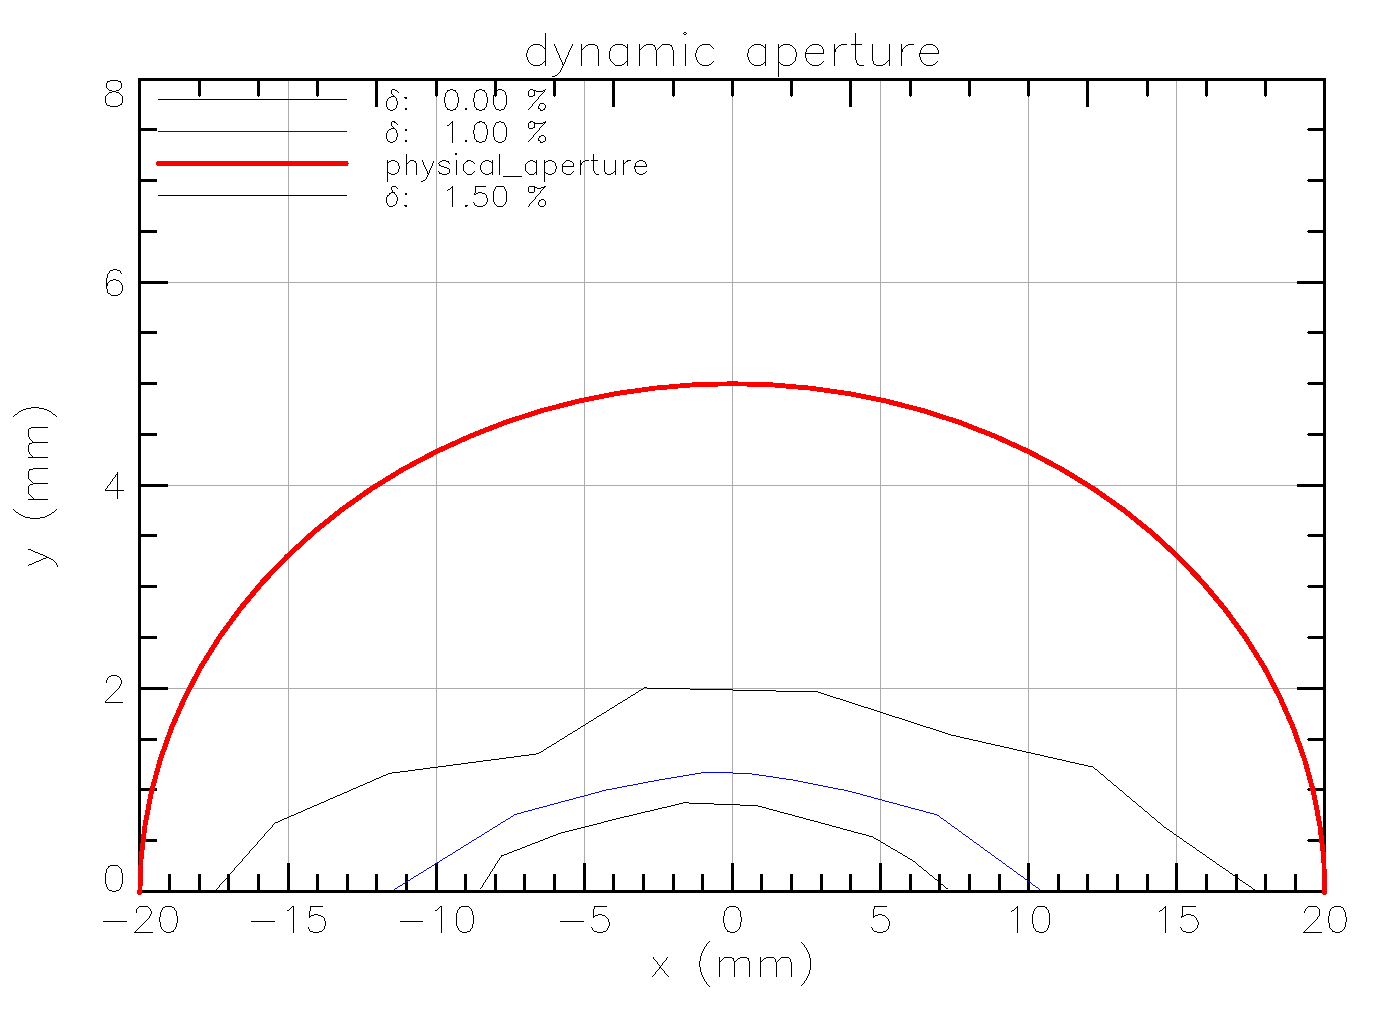
\includegraphics[width=5in]{dynamic-aperture.pdf}
  \caption{Example dynamic aperture plot.}
  \label{f:dynamic-aperture}
\end{figure}

A \vn{dynamic_aperture} drawing displays the results of the dynamic aperture
calculation. For example, the template
\begin{example}
&tao_template_plot
  plot%name = 'da'
  plot%x%min = -20
  plot%x%max =  20
  plot%x%major_div_nominal = 10
  plot%x%label = 'x (mm)'
  plot%x_axis_type = 'phase_space'
  plot%n_graph = 1
/

&tao_template_graph
  graph%name = 'g1'
  graph%type = 'dynamic_aperture'
  graph_index = 1
  graph%title = 'dynamic aperture'
  graph%margin =  0.15, 0.06, 0.12, 0.12, '%BOX'
  graph%x_axis_scale_factor = 1000
  graph%y%label = 'y (mm)'
  graph%y%label_offset = .2
  graph%y%max = 0
  graph%y%min = 0
  graph%y%major_div = 4
  graph%n_curve = 3
  curve(1)%y_axis_scale_factor = 1000
  curve(2)%y_axis_scale_factor = 1000
  curve(3)%y_axis_scale_factor = 1000
  curve(1)%draw_symbols = F
  curve(2)%draw_symbols = F
  curve(3)%draw_symbols = F
  curve(3)%data_type = 'physical_aperture'
  curve(3)%line%color = 2
  curve(3)%line%width = 5 
/
\end{example}
produces the plot on Fig.~\ref{f:dynamic-aperture}.  Each curve represents a single
momentum calculation according to \sref{s:dynamicaperture}.  If there are more momenta
than curves (as in this case), additional curves will automatically be created using the
styles of the previous curves. Note that apertures are calculated at element 0. If
\vn{curve(i)%ix_ele_ref} is nonzero, then the aperture will be propagated to this element.

Dynamic aperture curves can have the following \vn{%data_type}:
\begin{example}
  'dynamic_aperture' or ''    ! (default) points include the reference orbit
  'dynamic_aperture_centered' ! points are centered (relative to) the reference orbit
  'physical_aperture'         ! draws the physical aperture based on x1_limit, etc. 
\end{example}




%-----------------------------------------------------------------
\subsection{Drawing a Histogram}
\index{histogram drawing}
\label{s:histogram}



A \vn{histogram} drawing displays a histogram of phase space beam
density. Histogram plotting is associated with a \vn{graph} by setting
\vn{graph%type} equal to \vn{"histogram"}. The concepts here are
similar to \vn{phase space} plotting (\sref{s:phase.space}). An example is shown in
Fig.~\ref{f:histogram}, using the example
histogram template:
\begin{example}
&tao_template_plot
  plot%name = 'zhist'
  plot%x%min = -6
  plot%x%max =  6
  plot%x%label = 'z (mm)'	
  plot%n_graph = 1
/

&tao_template_graph
  graph_index = 1
  graph%name = 'z'
  graph%type = 'histogram'
  graph%box = 1, 1, 1, 1
  graph%title = 'Bunch Histogram: Z'
  graph%margin =  0.15, 0.06, 0.12, 0.12, '%BOX'
  graph%y%label = 'Current (A)'
  graph%n_curve = 1
  graph%y%label_offset = .1
  graph%x_axis_scale_factor = 1000.00 !m->mm

  curve1%hist%density_normalized = T
  curve1%hist%weight_by_charge = T
  curve1%hist%number = 100
  curve1%line%color = 4
  curve1%line%pattern = 2
  curve1%y_axis_scale_factor = 299792458  !Q/m * c_light
  curve1%data_type = 'z' 
  curve1%data_source = 'beam_tracking'
  curve1%ele_ref_name = "BEGINNING"
  curve1%symbol%type = 1
/
\end{example}

\begin{figure}
  \centering
  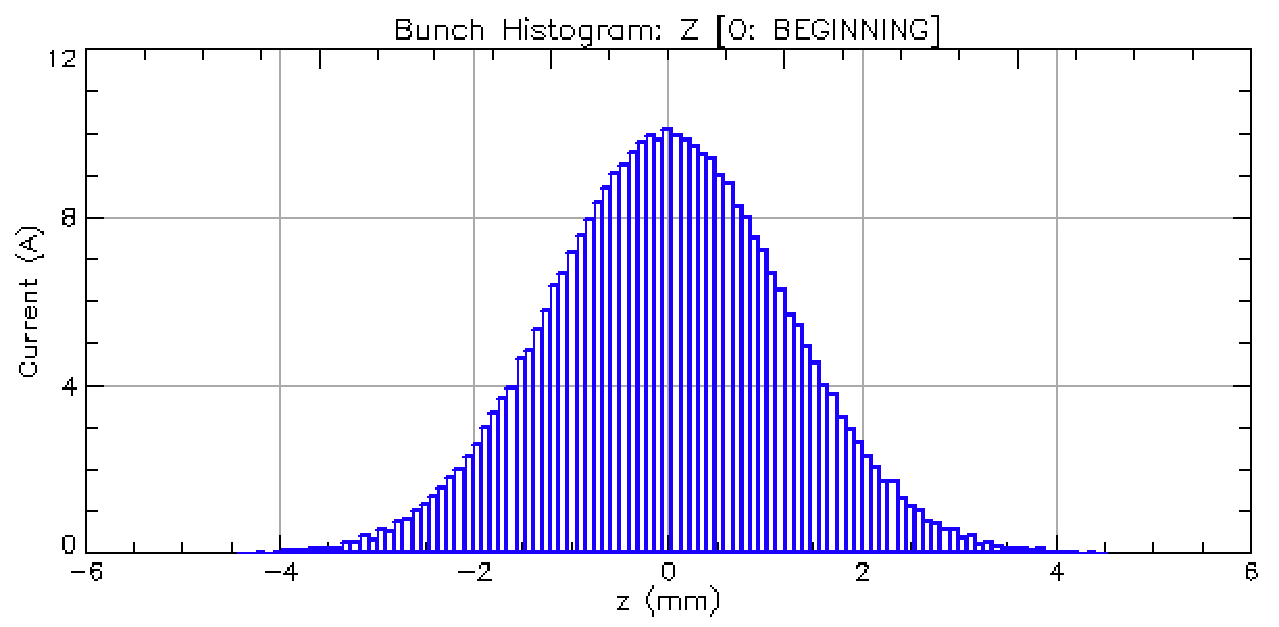
\includegraphics[width=5in]{histogram.pdf}
  \caption{Example histogram plot.}
  \label{f:histogram}
\end{figure}

For a \vn{"histogram"} type graph, \vn{curve%data_type} determines
what coordinate is plotted along the x-axis.
Valid \vn{curve%data_type} values are:
\index{x}\index{px}\index{y}\index{py}\index{z}\index{pz}
\begin{example}
  "x"
  "px"
  "y"
  "py"
  "z"
  "pz"
  "intensity"       -- Photon total intensity 
  "intensity_x"     -- Photon intensity along x-axis 
  "intensity_y"     -- Photon intensity along y-axis
  "phase_x"         -- Photon phase along x-axis
  "phase_y"         -- Photon phase along y-axis
\end{example}
In this example above, the $x$-axis of the plot will correspond to the
$z$ phase space coordinate.

The maximum and minimum of the bins is set automatically to fit the data.
The \vn{curve%hist%number} establishes the number of bins. Alternatively, 
if \vn{curve%hist%number = 0}, then \vn{curve%hist%width}  establishes
 the width of the histogram bins and sets the number automatically. 

If \vn{curve%hist%density_normalized = T}, then the height of a bin will be
divided by its width. If \vn{curve%hist%weight_by_charge = T}, then the particle
charge will be used to bin, otherwise the particle count will be used to bin.

The \vn{curve%hist%center} will insure that a bin will be centered at this location.

\index{curve!ele_ref_name}\index{curve!ix_ele_ref}
To change the place in the lattice where the data for the
\vn{histogram} is evaluated, use the \vn{set curve ele_ref_name} or
\vn{set curve ix_ele_ref} commands.

If \vn{graph%type} is \vn{"histogram"} then \vn{curve%data_source} 
must be either:
\begin{example}
  "beam"
  "multi_turn_orbit"
\end{example} 
\vn{"beam"} indicates that the points of the histogram plot
will be obtained correspond to the positions of the particles within a
tracked beam. \vn{multi_turn_orbit"} is used for rings where a single
particle is tracked multiple turns and the position of this particle
is recorded each turn. In this case, a \vn{d2_data} structure must
have been set up to hold the turn--by--turn orbit. This \vn{d2_data}
structure must be called \vn{multi_turn_orbit} and must have
\vn{d1_data} data arrays for the histogram planes to be plotted. For
example, if the histogram plot is \vn{x} versus \vn{px}, then there
must be \vn{d1_data} arrays named \vn{"x"} and \vn{"px"}. The number
of turns is determined by the setting of \vn{ix_max_data} in the
\vn{tao_d1_data} namelist (\sref{s:init.data}).

%-----------------------------------------------------------------
\subsection{Drawing the Beam Chamber Wall}
\index{beam chamber wall}
\label{s:beam.wall.draw}

If a beam chamber wall has been defined in the lattice file, This wall
can be drawn in a \vn{curve} by setting \vn{curve%type} to
\vn{"beam_chamber_wall"}.

Beam chamber walls are drawn, like a \vn{lat_layout}, on a one
dimensional line as a function of longitudinal position along the
machine centerline.

Note: Use the command \vn{show ele -wall} to print information about the
beam chamber wall for a particular element.

%-----------------------------------------------------------------
\subsection{Drawing a Key Table}
\index{key table}
\label{s:key.table}

The \vn{key table} is explained more fully in
Section~\sref{s:key.bind}.  An example is shown in
Figure~\ref{f:layout.table}. A template to create a key table looks
like:
\begin{example}
  &tao_template_plot
    plot%name = "table" 
    plot%n_graph = 1
  /

  &tao_template_graph
    graph%type = "key_table" 
    graph_index = 1
    graph%n_curve = 0
  /
\end{example}

The number in the upper left corner, to the left of the first column, 
(\vn{1} in Fig.~\ref{f:layout.table})
shows the active \vn{key bank}. The columns in the Key Table are:
\begin{example}
  Ix         ! Key index.
  Name       ! Element name whose attribute is bound.
  Attrib     ! Name of the element attribute that is bound.
  Value      ! Current value of bound attribute.
  Value0     ! Initial value of bound attribute.
  Delta      ! Change in value when the appropriate key is pressed.
  Uni        ! Universe that contains the element.
  Opt        ! Shows if bound attribute is used in an optimization.
\end{example}

Note that in a \vn{Lattice Layout}, if a displayed element has a bound
attribute, then the key index number will be displayed just above the
element's glyph.

The \vn{key_table} is drawn with respect to the upper left hand corner
of the region in which it is placed.

%-----------------------------------------------------------------
\subsection{Phase Space Plotting}
\index{phase space plotting}
\label{s:phase.space}

\begin{figure}
  \centering
  \begin{subfigure}[b]{0.45\textwidth}
    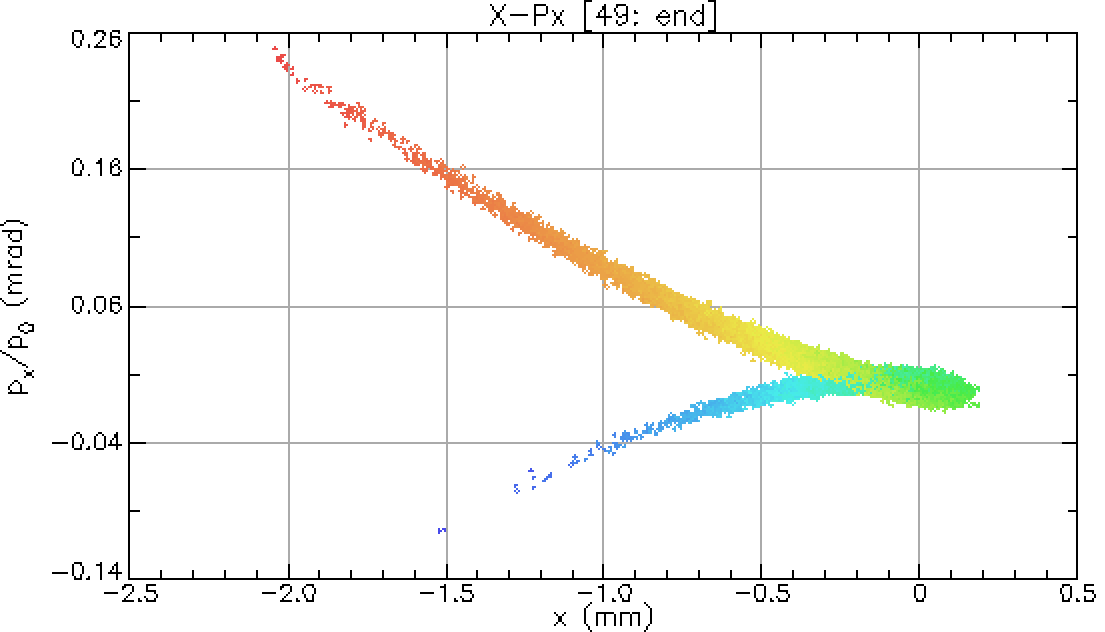
\includegraphics[width=\textwidth]{plot-color-xpx}
    \caption{Horizontal phase space}
  \end{subfigure}
  \begin{subfigure}[b]{0.45\textwidth}
    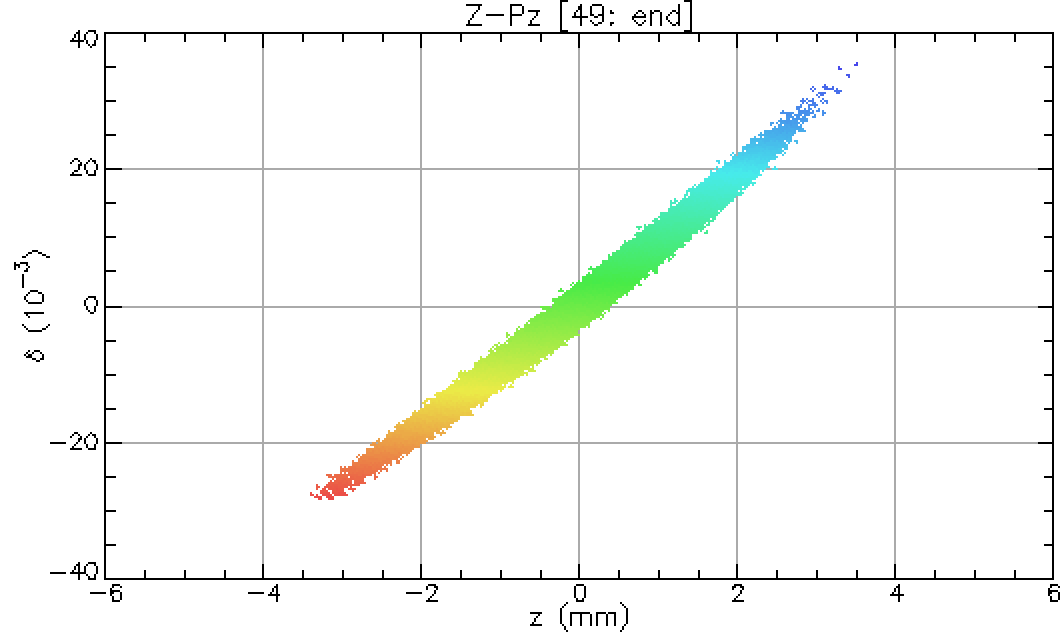
\includegraphics[width=\textwidth]{plot-color-zpz}
    \caption{Longitudinal phase space}
  \end{subfigure}  
  \caption{Example Phase Space plot, with points colored by the \vn{pz} coordinate.}
  \label{f:phase.space}
\end{figure}

A \vn{phase space} plot displays a particle or particles phase space
coordinates at a given location. Phase space plotting is associated
with a \vn{graph} by setting \vn{graph%type} equal to
\vn{"phase_space"}. The concepts here are similar to data plotting
(\sref{s:plot.data}). An example is show in Figure~\ref{f:phase.space}.
Example Phase Space template:
\begin{example}
&tao_template_plot
  plot%name = "xphase"
  plot%x%min =   -2.5
  plot%x%max = 0.5
  plot%x%label = "x (mm)"
  plot%n_graph = 1
/

&tao_template_graph
  graph_index = 1
  graph%name = "x"
  graph%type = "phase_space"
  graph%box = 1, 1, 1, 1
  graph%title = "X-Px"
  graph%margin =  0.15, 0.06, 0.12, 0.12, "%BOX"
  graph%x_axis_scale_factor = 1000.00 !m->mm
  graph%y%label =  "p\textbackslash{}dx\textbackslash{}u/p\textbackslash{}d0\textbackslash{}u (mrad)"
  graph%y%major_div = 4
  graph%n_curve = 1
  graph%y%label_offset=.4
  curve(1)%data_type = "x-px" 
  curve(1)%y_axis_scale_factor = 1000 !rad->mrad
  curve(1)%data_source = "beam_tracking"
  curve(1)%ele_ref_name = "END"
  curve(1)%symbol%type = 1
  curve(1)%data_type_z = "pz"
  curve(1)%use_z_color = T
  /
\end{example}

For a \vn{"phase_space"} type graph, \vn{curve%data_type_x} determines
what phase space coordinate is plotted along the x-axis and
\vn{curve%data_type} determines what phase space coordinate is plotted
along the y-axis. The phase space coordinates are:
\index{x}\index{px}\index{y}\index{py}\index{z}\index{pz}
\begin{example}
  "x"
  "px"
  "y"
  "py"
  "z"
  "pz"
  "intensity"       -- Photon total intensity 
  "intensity_x"     -- Photon intensity along x-axis 
  "intensity_y"     -- Photon intensity along y-axis
  "phase_x"         -- Photon phase along x-axis
  "phase_y"         -- Photon phase along y-axis
\end{example}
In this example above, the $x$-axis of the plot will correspond to the
$z$ phase space coordinate and the $pz$-axis will correspond to the
$px$ coordinate.

\index{curve!ele_ref_name}\index{curve!ix_ele_ref}
To change the place in the lattice where the data for the
\vn{phase_space} curve is evaluated, use the \vn{set curve
ele_ref_name} or \vn{set curve ix_ele_ref} commands.

Points can be colored by another phase space coordinate by activating
\vn{use_z_color = T}. 
The available curve options and defaults are:
\begin{example}
  use_z_color = F
  data_type_z = "" 
  z_color0 = 0
  z_color1 = 0
  autoscale_z_color = T
\end{example}
These can be the init file, or in Tao using the \vn{set curve} command. 
The \vn{data_type_z} can be set to any of the available phase space coordinates.
\vn{z_color0} and \vn{z_color1} specify the minimum and maximum of this coordinate
to be used in the color range. Values above or below this range will be colored
Black or Grey, respectively. 
If \vn{autoscale_z_color=T}, then these will be set automatically based on the
limits of the \vn{data_type_z} coordinate. 

If \vn{graph%type} is \vn{"phase_space"} then \vn{curve%data_source} 
must be either:
\begin{example}
  "beam"
  "multi_turn_orbit"
  "twiss"
\end{example} 
\vn{"beam"} indicates that the points of the phase space plot
will be obtained correspond to the positions of the particles within a
tracked beam. \vn{multi_turn_orbit"} is used for rings where a single
particle is tracked multiple turns and the position of this particle
is recorded each turn. In this case, a \vn{d2_data} structure must
have been set up to hold the turn--by--turn orbit. This \vn{d2_data}
structure must be called \vn{multi_turn_orbit} and must have
\vn{d1_data} data arrays for the phase space planes to be plotted. For
example, if the phase space plot is \vn{x} versus \vn{px}, then there
must be \vn{d1_data} arrays named \vn{"x"} and \vn{"px"}. The number
of turns is determined by the setting of \vn{ix_max_data} in the
\vn{tao_d1_data} namelist (\sref{s:init.data}). Using \vn{"twiss"} as
the \vn{curve%data_source} indicates that the phase space plot will be
an ellipse whose shape is based upon the Twiss and coupling
parameters, and the normal mode emittances. If the normal mode
emittances have not been computed then a nominal value of 1e-6~m-rad
is used.


\chapter{Tao Line Mode Commands}
\label{c:command}

\tao has two \vn{modes} for entering commands. In \vn{Line Mode}, described in this
chapter, \tao waits until the \vn{return} key is depressed to execute a command. That is,
a command consists of a single line of input. Conversely, \vn{Single Mode}, which is
described in Chapter~\sref{c:single}, interprets each keystroke as a command. Single Mode
is useful for quickly varying parameters to see how they affect a lattice but the number
of commands in Single Mode is limited. To put \tao into \vn{single mode} use the
\vn{single_mode} command (\sref{s:sing}).

\index{commands!Command List} 
Commands are case sensitive. The list of commands is shown in
Table~\ref{t:commands}. Multiple commands may be entered on one line using the semicolon
``;'' character as a separator.  [However, a semicolon used as as part of an \vn{alias}
(\sref{s:alias}) definition is part of that definition.]  An exclamation mark ``\vn{!}''
denotes the beginning of a comment and the exclamation mark and everything after it to the
end of the line is ignored.  Example:
\begin{example}
  set default uni = 2; show global  ! Two commands and a comment
\end{example}

This chapter uses the following special characters to define the command line syntax:
\begin{example}
  \{\}        ! Identifies an optional argument. 
              !   Arguments now enclosed in brackets are required
  <>        ! Indicates a non-literal argument.
\end{example}

Example:
\begin{example}
  change \{-silent\} variable <name>[<locations>] <number>
\end{example}
Here the \vn{-silent} argument is optional while the \vn{variable} argument is
mandatory. Appropriate values for \vn{<name>}, \vn{<locations>}, and \vn{<number>} must be
substituted. A possible

\begin{example}
  change var steering[34:36] @1e-3  ! set the steering strength #34-36 to 0.001
\end{example}

%% command_table -----------------------------------------------------

\begin{table}[h]
\centering {\tt
\begin{tabular}{|l|l||l|l|} \hline
  {\it Command} & {\it Section}     & {\it Command} & {\it Section}     \\ \hline
  alias         & \sref{s:alias}    & re_execute    & \sref{s:re.exe}   \\ \hline
  call          & \sref{s:call}     & read          & \sref{s:read}     \\ \hline
  change        & \sref{s:change}   & restore       & \sref{s:restore}  \\ \hline 
  clip          & \sref{s:clip}     & reinitialize  & \sref{s:reinit}   \\ \hline 
  continue      & \sref{s:continue} & run_optimizer & \sref{s:run}      \\ \hline 
  derivative    & \sref{s:deriv}    & scale         & \sref{s:scale}    \\ \hline 
  do, enddo     & \sref{s:do}       & set           & \sref{s:set}      \\ \hline  
  end_file      & \sref{s:end.file} & show          & \sref{s:show}     \\ \hline 
  exit          & \sref{s:exit}     & single_mode   & \sref{s:sing}     \\ \hline 
  flatten       & \sref{s:flatten}  & spawn         & \sref{s:spawn}    \\ \hline 
  help          & \sref{s:help}     & timer         & \sref{s:timer}    \\ \hline
  misalign      & \sref{s:misalign} & use           & \sref{s:use}      \\ \hline 
  pause         & \sref{s:pause}    & veto          & \sref{s:veto}     \\ \hline 
  place         & \sref{s:place}    & value         & \sref{s:value}    \\ \hline
  plot          & \sref{s:plot}     & wave          & \sref{s:wave}     \\ \hline
  ptc           & \sref{s:ptc}      & write         & \sref{s:write}    \\ \hline 
  python        & \sref{s:python}   & x_axis        & \sref{s:x.axis}   \\ \hline 
  quiet         & \sref{s:quiet}    & x_scale       & \sref{s:x.scale}  \\ \hline 
  quit          & \sref{s:quit}     & xy_scale      & \sref{s:xy.scale} \\ \hline
\end{tabular}}
\caption{Table of \tao commands.}
\label{t:commands}
\end{table}

%% Marker: "help" will not display anything after this  -----------

\vfil
\break

%% alias --------------------------------------------------------------
\section{alias}\index{commands!alias}
\label{s:alias}

The \vn{alias} command defines command shortcuts. Format:
\begin{example}
  alias \{<alias_name> <string>\}
\end{example}

\vskip 0.1in

\vn{Alias} is like Unix aliases. Using the \vn{alias} command without any arguments
results in a printout of the aliases that have been defined. When using an alias up to 9
arguments may be substituted in the \vn{<string>}. The i\Th argument is substituted in
place of the sub-string ``[[i]]''.  arguments that do not have a corresponding ``[[i]]''
are placed at the end of \vn{<string>}.

Aliases can be set up for multiple commands using semicolons.

Examples:
\begin{example}
    alias xyzzy plot [[1]] model  ! Define xyzzy
    alias                         ! Show all aliases
    xyzzy top                     ! Use an alias
    plot top model                ! Equivalent to "xyzzy top"
    xyzzy top abc                 ! Equivalent to "plot top model abc"
    alias foo  show uni; show top ! "foo" equivalent to "show uni; show top"
\end{example}
In the above example ``xyzzy'' is the alias for the string ``plot [[1]] model''.  When the
command xyzzy is used ``top'' is substituted for ``[[1]]'' in the string.

%% call --------------------------------------------------------------
\section{call}\index{commands!call}
\label{s:call}

The \vn{call} command opens a command file (\sref{s:command.files}) and executes the
commands in it.  Format:
\begin{example}
  call <filename> \{<arg_list>\}  \Strut
  call -ptc <filename>
\end{example}

\vskip 0.2in 
\tao first looks in the current directory for the command file.

The \vn{call} command without \vn{-ptc} is for running a set of \tao commands.  Up to 9
arguments may be passed to the command file. The i\Th argument is substituted in place of
the string ``[[i]]'' in the file. Nesting of command files (command files calling other
command files) is allowed. There is no limit to the number of nested files.  See
Section~\sref{s:command.files} for more details.

The \vn{call -ptc} command passes the command file to PTC for processing. Previous to such
a call, the command \vn{ptc init} must be issued.

If the command file has the \vn{quiet} command in it, output to the terminal is surpresed (but
only for the duration of the execution of the file).

Command loops can be implemented in a command file. See Section~\sref{s:do} for more details.

Other useful commands to put in a command file are to speed up execution are:
\begin{example}
  set global lattice_calc_on = F   ! Stop lattic calculations
  set global plot_on = F           ! Halt replotting
\end{example}
If set, at the end of the command file these logicals should be toggled back to True.

Examples:
\begin{example}
    call my_cmd_file abc def 
\end{example}
In the above example the argument ``abc'' is substituted for any ``[[1]]'' appearing the
file and ``def'' is substituted for any ``[[2]]''.  \Newline

%% change --------------------------------------------------------------
\section{change}\index{commands!change}
\label{s:change}

The \vn{change} command changes element attribute values or variable values in the
\vn{model} lattice. Format:
\begin{example}
  change element <element_list> <attribute> \{prefix>\} <number>
  change \{-silent\} variable <name>[<locations>] \{<prefix>\} <number>
  change  \{n@\}beam_start <coordinate> \{prefix>\} <number>
\end{example}

\vskip 0.2in 

The \vn{change} is used for changing real (as opposed to integer or logical)
parameters. Also see the \vn{set} command (\sref{s:set}) which is more general.

If \vn{<prefix>} is not present, \vn{<number>} is added to the existing value
of the attribute or variable. That is:
\begin{example}
  final_model_value = initial_model_value + <number>
\end{example}
If \vn{<prefix>} is present, it may be one of
\begin{example}
  @       final_model_value = <number>
  d       final_model_value = design_value + <number>
  \%       final_model_value = initial_model_value * (1 + <number> / 100)
\end{example}

Element list format (\sref{s:ele.list.format}), without any embedded blanks, is used for
the \vn{<element_list>} argument.

For \vn{change beam_start}, The optional \vn{n@} universe specification
(\sref{s:universe}) may be used to specify the universe or universes to apply the change
command to.

For lattices with an open geometry, \vn{change beam_start <coordinate> <number>} can be
used to vary the starting coordinates for single particle tracking or the centroid
coordinates for beam tracking. Here \vn{<coordinate>} is one of:
\begin{example}
  x, px, y, py, z, pz, t
\end{example}
For photons, \vn{<coordinate>} may also be:
\begin{example}
  field_x, field_y, phase_x, phase_y
\end{example}
For closed lattices only the \vn{pz} component is applicable. For lattices that have an
\vn{e_gun} (which necessarily implies that the lattice has an open geometry), the time
\vn{t} coordinate must be varied instead of \vn{pz}.

For open lattices, \vn{change element beginning <twiss>} can be used to vary the starting
Twiss parameters where \vn{<twiss>} is one of:
\begin{example}
  beta_a, beta_b, alpha_a, alpha_b 
  eta_a, eta_b,etap_a, etap_b    
\end{example}

The \vn{-silent} switch, if present, suppresses the printing of what variables are
changed.

Examples:
\begin{example}
  change ele 3@124 x_offset 0.1        ! Offset element #124 in universe 3 by 0.1
  change ele 1,3:5 x_offset 0.1        ! Offset elements 1, 3, 4, and 5 by 0.1
  change ele q* k1 d 1.2e-2            ! Set the k1 strength of all elements starting with
                                       !   the letter "q" relative to the design
  change ele quadrupole::* k1 d 1.2e-2 ! Set the k1 strength of all quadrupole elements.
  change var steering[34:36] @1e-3     ! set the steering strength #34-36 to 0.001
  change var steering[*] \%10           ! vary all steering strengths by 10\%
  change 2@beam_start x @0.001         ! set beginning x position in universe 2 to 1 mm.
\end{example}


%% clip --------------------------------------------------------------
\section{clip}\index{commands!clip}
\label{s:clip}

The \vn{clip} command vetoes data points for plotting and optimizing. That is, the
\vn{good_user} logical of the data associated with the out-of-bound plotted points are set
to False.  Format:
\begin{example}
  clip \{-gang\} \{<where> \{<limit1> \{<limit2>\}\}\}
\end{example}

\vskip 0.2in 

Which graphs are clipped is determined by the \vn{<where>} switch. If \vn{<where>} is not
present, all graphs are clipped. If \vn{where} is a plot name, then all the graphs of that
plot are clipped. If \vn{where} is the name of a \vn{d2_data} (for example, \vn{orbit}) or
a \vn{d1_data} (for example, \vn{orbit.x}) structure, then those graphs that display this
data are clipped.

The points that are clipped those points whose $y$ values are outside a certain range
defined by \vn{<limit1>} and \vn{<limit2>}. If neither \vn{<limit1>} nor \vn{<limit2>} are
present, the clip range is taken to be outside the graph minimum and maximum $y$--axis
values. If only \vn{<limit1>} is present then the clip range is outside the region from
-\vn{<limit1>} to +\vn{<limit1>}. If both are present than the range is from \vn{<limit1>}
to \vn{<limit2>}.

The \vn{-gang} switch is apply a clip to corresponding data in a \vn{d2_data} structure.
For example
\begin{example}
  clip -g orbit.x   ! Clips both orbit.x and orbit.y 
\end{example}
Here the \vn{orbit.x} data is clipped and the corresponding data in \vn{orbit.y} is also
vetoed. For example, if datum number 23 in \vn{orbit.x} is clipped, datum number 23 in
\vn{orbit.y} will be vetoed.

Examples:
\begin{example}
  clip top.x -3  7  ! Clip the curves in the x graph in the top region
  clip bottom       ! Clip the graphs in the bottom region
  clip -g orbit.x   ! Clip the 
\end{example}

%% continue --------------------------------------------------------------
\section{continue}\index{commands!continue}
\label{s:continue}

The \vn{continue} command is used to continue reading of a suspended command file
(\sref{s:command.files}) after a \vn{pause} command (\vn{s:pause}). Format:
\begin{example}
  continue
\end{example}

%% do --------------------------------------------------------------
\section{do, enddo}\index{commands!do}
\label{s:do}

Command loops can be implemented in a command file files. Format:
\begin{example}
  do <var> = <l_bound>, <u_bound> \{<incr>\}
    ...   ! use the syntax ``[[<var>]]'' to refer to a variable.
  enddo
\end{example}
Note: ``\vn{enddo}'' is one word and my not be split into two words.
Loops can be nested and the number of levels is not unlimited. 

A loop will execute the code in between the \vn{do} and \vn{enddo} lines a certain number of
times. Each time trough the the the integer variable \vn{<var>} will be increamented by \vn{<incr>},
starting at \vn{<l_bound>} and stopping before \vn{<var>} is greater than \vn{<u_bound>}. If
\vn{<incr>} is not present, the increment will be 1. Note: \vn{<l_bound>}, \vn{<u_bound>}, and
\vn{<incr>} must all be integers.

Example:
\begin{example}
  do j = 0, 10, 2
    set beam_start pz = 1e-3 * [[j]]
    ...
  enddo
\end{example}
As shown in the above example, to refer to a loop variable in a command, use the syntax ``[[<var>]]''.

%% end_file --------------------------------------------------------------
\section{end_file} \label{s:end.file}
\index{commands!end_file}

The \vn{end_file} command is used in command files (\sref{s:command.files}) to signal the
end of the file. Everything after an \vn{end_file} command is ignored. An \vn{end_file}
command entered at the command line will simply generate an error message.  Format:
\begin{example}
  end_file
\end{example}

%% exit --------------------------------------------------------------
\section{exit}\index{commands!exit}
\label{s:exit}

The \vn{exit} command exits the program. Same as \vn{Quit}.  Format:
\begin{example}
  exit
\end{example}

%% derivative --------------------------------------------------------------
\section{derivative}\index{commands!derivative}
\label{s:deriv}

The \vn{derivative} command calculates the \vn{dModel_Data/dVar} derivative matrix needed
for the \vn{lm} optimizer.  Format:
\begin{example}
  derivative
\end{example}

%% flatten --------------------------------------------------------------
\section{flatten}\index{commands!flatten}
\label{s:flatten}

The \vn{Flatten} command runs the optimizer to minimize the merit function. This is the
same as the \vn{run_optimizer} command.  See the \vn{run_optimizer} command for more
details.  Format:
\begin{example}
  flatten \{<optimizer>\}
\end{example}

\vskip 0.2in

%% help --------------------------------------------------------------
\section{help}\index{commands!help}
\label{s:help}

The \vn{help} command gives help on \tao commands. Format:
\begin{example}
  help \{<command> \{<subcommand>\}\}
\end{example}

\vskip 0.2in

The \vn{help} command without any arguments gives a list of all commands.  Some commands,
like \vn{show}, are so large that help on these commands is divided up by their
subcommand.

Examples:
\begin{example}
  help            ! Gives list of commands.
  help run        ! Gives help on the run_optimizer command.
  help show       ! Help on the show command.
  help show alias ! Help on the show alias command.
\end{example}

Note: The \vn{help} command works by parsing the file \vn{\$TAO_DIR/doc/command-list.tex}
which is the LaTeX file for the Line Mode Commands chapter of the \tao manual. Thus, for
the \vn{help} command to work properly, the environmental variable \vn{TAO_DIR} must be
appropriately defined. Generally, \vn{TAO_DIR} will be defined if the appropriate setup
script has been run. For ``Distributions'', this is the same setup script used to setup a
distribution. See your local \bmad guru for details.

%% misalign --------------------------------------------------------------
\section{misalign}\index{command!misalign}
\label{s:misalign}

The \vn{misalign} command misaligns a set of lattice elements. Format:
\begin{example}
   misalign <wrt> <ele_type> <range> <ele_attrib> <misalign_value>
\end{example}

\vskip 0.2in 

\vn{<ele_type>} is the type of element to misalign.  Only elements of type \vn{<ele_type>}
will be misaligned within the range.  If \vn{<ele_type>} begins with "*@" then choose all
universes. If \vn{<ele_type>} begin with "n@" then choose universe n. Otherwise the
default universe (\sref{s:universe})) is used.

A lattice element will only be misaligned if its lattice index falls within a range given
by \vn{<range>}. \vn{<range>} is of the form \vn{nnn:mmm} or the word \vn{ALL}.

The element attribute \vn{<ele_attrib>} is ``misaligned'' by the rms value
\vn{<misalign_value>} with respect to the setting of \vn{<wrt>}. Any element attribute can
be misaligned provided the attribute is free to vary.

If \vn{<misalign_value>} is prepended by 'x' then the misalignment value will be a
relative misalignment with respect to the \vn{<wrt>} value. Otherwise, it's an absolute
rms value about the \vn{<wrt>} value.

In the special case where sbend strengths are misaligned then use \vn{<ele_attrib> =
g_err}. However, if a relative error is specified it will be relative to 'g'.

The possible values of \vn{<wrt>} are:
\begin{example}
  wrt_model          ! Misalign about the current model value
  wrt_design         ! Misalign about the design value
  wrt_survey         ! Misalign about the zero value
\end{example}

Examples
\begin{example}
   ! The following will misalign all quadrupole vertical positions in the default
   ! universe within the lattice element range 100:250 with respect to the zero 
   ! value by 300 microns
  misalign wrt_survey quadrupole 100:250 y_offset 300e-6
   ! The following will misalign all quadrupole strengths in all universes for
   ! the entire lattice with respect to the design value by 1%.
  misalign wrt_design *@quadrupole ALL k1 x0.01
\end{example}

%% pause --------------------------------------------------------------
\section{pause}\index{commands!pause}
\label{s:pause}

The \vn{pause} command is used to pause \tao when executing a command file
(\sref{s:command.files}). Format:
\begin{example}
  pause \{<time>\} ! Pause time in seconds.
\end{example}
\vskip 0.2in

If \vn{<time>} is not present or zero, \tao will pause until the \vn{CR} key is
pressed. Once the \vn{CR} key is pressed, the command file will be resumed. If \vn{<time>}
is negative, \tao will suspend the command file. Commands can now be issued from the
keyboard and the command file will be resumed when a \vn{continue} command
(\sref{s:continue}) is issued. Multiple command files can be simultaneously suspended.
Thus, while one command file is suspended, a second command file can be run and this
command file too can be suspended. A \vn{continue} command will resume the second command
file and when that command file ends, another \vn{continue} command will be needed to
complete the first suspended command file. Use the \vn{show global} command to see the
number of suspended command files.

Example:
\begin{example}
  pause 1.5    ! Pause for 1.5 seconds.
  pause -1     ! Suspend the command file until a \vn{continue} 
               !   command is issued.
\end{example}

%% place --------------------------------------------------------------
\section{place}\index{commands!place}
\label{s:place}

The \vn{place} command is used to associate a \vn{<template>} plot with a \vn{<region>}
and thus create a visible plot in that region. Format:
\begin{example}
  place <region> <template>
  place <region> none
  place * none
\end{example}

\vskip 0.2in 

To erase a plot from a region use \vn{none} in place of a template name. Notice that by
using multiple \vn{place} commands a \vn{template} can be associated with more than one
region.  \vn{place * none} will erase all plots.

Examples:
\begin{example}
  place top orbit  ! place the orbit template in the top region
  place top none   ! erase any plots in the top region
\end{example}

%% plot --------------------------------------------------------------
\section{plot}\index{commands!plot}
\label{s:plot}

The \vn{plot} command is used to determine what ``components'' (\sref{s:plot.data}) are
plotted in the specified graphs or plots. Format:
\begin{example}
  plot <plot_or_graph> <component>
\end{example}

\vskip 0.2in 

components are a property of a graph (or curve) so when <plot_or_graph> specifies a plot,
all the graphs associated with the plot are assigned the \vn{<component>}.

Note: The plot command is a shortcut for the commands:
\begin{example}
  set plot <plot_name> component = <component>     ! and
  set graph <graph_name> component = <component>
\end{example}
Also see the \vn{set curve} command.

Use a ``-'' for baselines. 

Examples:
\begin{example}
  plot bottom.g1 model - design        ! Plot model - design in the g1 graph of the bottom region
  plot top meas - model + design - ref ! Set the components for the graphs in the top region.
\end{example}

%% ptc -----------------------------------------------------------
\section{ptc}\index{commands!ptc}
\label{s:ptc}

The \vn{ptc} command is used manipulating PTC layouts associated with Bmad
lattices. Format:
\begin{example}
  ptc init            ! Init associated PTC layout.
\end{example}

\vskip 0.2in 

The \vn{ptc init} command must be run before running any other \vn{ptc} command is used.

Also see:
\begin{example}
  call -ptc <file>         ! Run a PTC script
  read ptc                 ! Read a PTC lattice
  write ptc                ! Write a PTC lattice
\end{example}

Examples:
\begin{example}
  ptc init
\end{example}

%% python -----------------------------------------------------------
\section{python}\index{commands!python}
\label{s:python}

The \vn{python} command is like the \vn{show} command in that the \vn{python} command
prints information to the terminal. The difference is that the output from the \vn{show}
command is meant for viewing by the user while the output of the \vn{python} command is
meant for easy parsing. Format:
\begin{example}
  python \{-append <file_name>\} \{-noprint\} <what_to_print>
  python \{-write <file_name>\} \{-noprint\} <what_to_print>
\end{example}

The \vn{python} command has \vn{-append} and \vn{-write} optional arguments which can be
used to write the results to a file. The \vn{python -append} command will appended to the
output file. The \vn{python -write} command will first erase the contents of the output
file. Example:
\begin{example}
  python -write d2.dat data_d2    ! Write to file "d2.dat"
\end{example}

The \vn{-noprint} option suppresses printing and is useful when writing large amounts of
data to a file.  The \vn{python} command can be used to pass information to a parent
process when \tao is run as a subprocess.  The parent process may be any scripting program
like Python, Perl, Tcl, etc.  In particular, see \sref{c:python} for details on how to run
\tao as a Python subprocess.

For long term maintainability of python scripts, the advantage of using the \vn{python}
command in the scripts over the \vn{show} command comes from the fact that the output
syntax of the \vn{show} command can (and does) change.

For further documentation on the python command, please look at the file tao/code/tao_python.f90.

Note: At this point in time, the \vn{python} command is still in development.  Please
contact David Sagan if needed.

%% quiet --------------------------------------------------------------
\section{quiet}\index{commands!quiet}
\label{s:quiet}

Format:
\begin{example}
  quiet
\end{example}

The \vn{quiet} command can only be used in command files (\sref{s:call}).
When placed in a command file, output to the terminal is surpresed (but
only from the \vn{quiet} command for the duration of the execution of the file).

Other useful commands to put in a command file are to speed up execution are:
\begin{example}
  set global lattice_calc_on = F   ! Stop lattic calculations
  set global plot_on = F           ! Halt replotting
\end{example}
If set, at the end of the command file these logicals should be toggled back to True.

%% quit --------------------------------------------------------------
\section{quit}\index{commands!quit}
\label{s:quit}

\vn{Quit} exits the program. Same as \vn{exit}.
Format:
\begin{example}
  quit
\end{example}

%% re_execute --------------------------------------------------------------
\section{re_execute}
\index{commands!re_execute}
\label{s:re.exe}

The \vn{re_execute} command reruns prior commands.  Format:
\begin{example}
  re_execute <index>   ! Re-execute a command with the given index number.
  re_execute <string>  ! Re-execute last command that begins with <string>.
\end{example}

\vskip 0.2in 
Every \tao command entered is recorded in a ``history stack''. These
commands can be viewed using the \vn{show history} command. The \vn{show_history}
command will also display the index number associated with each command.

Examples
\begin{example}
  re_exe 34   ! Re-execute command number 34.
  re_exe set  ! Re-execute last ``set'' command.  
\end{example}

%% read --------------------------------------------------------------
\section{read}\index{commands!read}
\label{s:read}

The \vn{read} command is used to modify the (\bmad) \vn{model} lattice or the associated
\vn{PTC} lattice.  Format:
\begin{example}
  read lattice <file_name>
  read ptc \{-old\} <file_name>
\end{example}

\vskip 0.2in 

With the \vn{read lattice} command, the \vn{model} lattice contained in the default
universe (\sref{s:universe}) is modified using a ``secondary'' lattice file.  [See the
\bmad manual for the definition of secondary.]

For example, with the appropriate file, the \vn{read} command can be used to misalign the
lattice elements. The input file must be in Bmad standard lattice format.

Note: Due to bookkeeping complications, the number of lattice elements may not be
modified. If it is desired to initiate \tao using both ``primary'' and secondary lattice
files, this can be done as illustrated in \sref{s:init.lat}.

The \vn{read ptc} command reads in a PTC lattice. WARNING: This command is
untested. Please contact David Sagan if you want to use it.

%% restore --------------------------------------------------------------
\section{restore}\index{commands!restore}
\label{s:restore}

The \vn{restore} command cancels data or variable
vetoes. Format:
\begin{example}
  restore data  <data_name> <locations>
  restore var <var_name> <locations>
\end{example}

\vskip 0.2in 

See also the \vn{use} and \vn{veto} commands.

Examples:
\begin{example}
  restore data orbit.x[23,34:56]   ! un-veto orbit.x 23 and 34 through 56.
  restore data orbit.x[23,34:56:2] ! un-veto orbit.x 23 and even data between 34 
                                   !                                          and 56
  restore data *@orbit[34]         ! un-veto orbit data in all universes.
  restore var quad_k1[67]          ! un-veto variable
\end{example}

%% reinitialize -------------------------------------------------------
\section{reinitialize}\index{commands!reinitialize}
\label{s:reinit}

The \vn{reinitialize} command reinitializes various things. Format:
\begin{example}
  reinitialize beam
  reinitialize data
  reinitialize tao \{command line optional arguments\}
\end{example}

\vskip 0.2in 

The \vn{reinitialize beam} command reinitializes the beam at the start of the
lattice. That is, a new random distribution is generated.  Note: This also reinitializes
the model data.

\vn{reinitialize data} forces a recalculation of the model data.  Normally, a
recalculation is done automatically when any lattice parameter is changed so this command
is generally only useful for debugging purposes.

\vn{reinitializes tao} reinitializes \tao. This can be useful to reset everything to
initial conditions or to perform analysis with more than one initialization file. See
section \sref{s:command.line} for a list of the optional arguments.  If an argument is not
set, the \vn{reinitialize} command uses the same argument value that were used in the last
\vn{reinitialize} command, or, if this is the first reinitialization, what was used to
start \tao.

Examples:
\begin{example}
  reinit tao                         ! Reinit using previous arguments
  reinit tao -init tao_special.init  ! Reinitializes \tao with the initialization file 
                                     !   tao_special.init
\end{example}


%% run --------------------------------------------------------------
\section{run_optimizer}\index{commands!run}
\label{s:run}

The \vn{run_optimizer} command runs an optimizer. Format:
\begin{example}
  run_optimizer \{<optimizer>\}
\end{example}

\vskip 0.2in 

\index{de!optimizer}\index{lm!optimizer}
If \vn{<optimizer>} is not given then the default optimizer is used. 
Use the \vn{show optimizer} (\sref{s:show.optimizer}) command to see optimizer parameters.
To stop the optimizer
before it is finished press the period ``.''  key. If you want the optimizer to run
forever run the optimizer in \vn{single mode}. Valid optimizers are:
\begin{example}
  de            ! Differential Evolution
  geodesic_lm   ! ``Geodesic'' Levenburg-Marquardt 
  lm            ! Levenburg-Marquardt from Numerical Recipes 
  lmdif         ! Levenburg-Marquardt 
\end{example}

See Chapter~\sref{c:opti} for details on how \tao structures optimization and 
for more details on the different optimizers.

Examples:
\begin{example}
  run         ! Run the default optimizer
  run de      ! Run the de optimizer
\end{example}

%% scale --------------------------------------------------------------
\section{scale}\index{commands!scale}
\label{s:scale}

The \vn{scale} command scales the vertical axis of a graph or set of graphs.  Format:
\begin{example}
  scale \{-y\} \{-y2\} \{-gang\} \{-nogang\} \{<where>\} \{<value1> \}<value2>\}\}\}
\end{example}

Which graphs are scaled is determined by the \vn{<where>} switch. If \vn{<where>} is not
present or \vn{<where>} is \vn{all} then all graphs are scaled. \vn{<where>} can be a plot
name or the name of an individual graph withing a plot.

\vskip 0.2in 

\vn{scale} adjusts the vertical scale of graphs. If neither \vn{<value1>} nor
\vn{<value2>} is present then an \vn{autoscale} is performed and the scale is adjusted so
that all the data points are within the graph region. If an autoscale is performed upon an
entire plot, and if \vn{plot%autoscale_gang_y} (\sref{s:template}) is True, then the
chosen scales will be the same for all graphs. That is, a single scale is calculated so
that all the data of all the graphs is within the plot region. The affect of
\vn{plot%autoscale_gang_y} can be overridden by using the \vn{-gang} or \vn{-nogang}
switches.

If only \vn{<value1>} is present then the scale is taken to be from -\vn{<value1>} to
+\vn{<value1>}. If both are present than the scale is from \vn{<value1>} to \vn{<value2>}.

A graph can have a \vn{y2} (left) axis scale that is separate from the \vn{y} (right)
axis. Normally, the \vn{scale} command will scale both axes.  Scaling of just one of these
axes can be achieved by using the \vn{-y} or \vn{-y2} switches.

Examples:
\begin{example}
  scale top.x -3  7  ! Scale the x graph in the top region
  scale -y2 top.x    ! Scale only the y2 axis of the top.x graph.
  scale bottom       ! Autoscale the graphs of the plot in the bottom region
  scale              ! Scale everything
\end{example}


%% set --------------------------------------------------------------
\section{set}\index{commands!set}
\label{s:set}


The \vn{set} command is used to set values for data,
variables, etc. Format:
\begin{example}
  set beam_init \{n@\}<component> = <value>                   ! \sref{s:set.beam.init}
  set beam_start \{n@\}<coordinate> = <value>                 ! \sref{s:set.beam.start}
  set bmad_com <component> = <value>                        ! \sref{s:set.bmad.com}
  set csr_param <component> = <value>                       ! \sref{s:set.csr.param}
  set curve <curve> <component> = <value>                   ! \sref{s:set.curve}
  set data <data_name>|<component> = <value>                ! \sref{s:set.data}
  set default <parameter> = <value>                         ! \sref{s:set.default}
  set element <element_list> <attribute> = <value>          ! \sref{s:set.element}
  set floor_plan <component> = <value>                      ! \sref{s:set.floor.plan}
  set geodesic_lm <component> = <value>                     ! \sref{s:set.geodesic.lm}
  set global <component> = <value>                          ! \sref{s:set.global}
  set graph <graph> <component> = <value>                   ! \sref{s:set.graph}
  set key <key> = <command>                                 ! \sref{s:set.key}
  set lat_layout <component> = <value>                      ! \sref{s:set.lat.layout}
  set lattice \{n@\}<destination\_lat> = <source\_lat>          ! \sref{s:set.lattice}
  set opti_de_param <component> = <value>                   ! \sref{s:set.opti.de.param}
  set plot <plot> <parameter> = <value>                     ! \sref{s:set.plot}
  set plot_page <parameter> = <value1> \{<value2>\}           ! \sref{s:set.plot.page}
  set ran_state = <random_number_generator_state>           ! \sref{s:set.ran.state}
  set universe <what_universe> <on/off>                     ! \sref{s:set.universe}
  set universe <what_universe> recalculate                  ! \sref{s:set.universe}
  set universe <what_universe> mat6_recalc <on/off>         ! \sref{s:set.universe}
  set universe <what_universe> track_recalc <on/off>        ! \sref{s:set.universe}
  set variable <var_name>|<component> = <value>             ! \sref{s:set.variable}
  set wave <component> = <value>                            ! \sref{s:set.wave}
\end{example}

\vskip 0.2in 

Also see the \vn{change} command (\sref{s:change}). The \vn{change} command is specialized
for varying real parameters while the \vn{set} command is more general.

Note: The \vn{show} command (\sref{s:show}) is able to display the settings of many variables
that can be set by the \vn{set} command.

To apply a set to all data or variable classes use ``*'' in place of \vn{<data_name>} or
\vn{var_name}.

To set the prompt color, use the command
\begin{example}
  set global prompt_color = <value>
\end{example}
Where \vn{<value>} may be one of:
\begin{example}
  'BLACK'
  'RED'
  'GREEN'
  'YELLOW'
  'BLUE'
  'MAGENTA'
  'CYAN'
  'GRAY'
  'DEFAULT'       ! Default foreground color
\end{example}

% Use the command:
%   help set <what>
% to obtain more information on a particular set subtopic. Example:
%   help set plot

%% set beam_init --------------------------------------------------------------

\subsection{set beam_init}
\label{s:set.beam.init}

Format:
\begin{example}
  set beam_init \{n@\}<component> = <value>
\end{example}

For \vn{set beam_init}, the \vn{<component>}s that can be set can be found in
section~\sref{s:beam.init}. The optional \vn{n@} allows the specification of the universe
or universes the set is applied to. The current default universe (\sref{s:universe}) will
be used if no universe is given. Use the \vn{show beam} command (\sref{s:show}) to see the
current values of the \vn{beam_init} structure.

Examples:
\begin{example}
  set beam_init 3@center(2) = 0.004  ! Set px center of beam for universe 3.
  set beam_init [1,2]@sig_e = 0.02   ! Set sig_e for universes 1 and 2.
\end{example}

%% set beam_start --------------------------------------------------------------

\subsection{set beam_start}
\label{s:set.beam.start}

Format:
\begin{example}
  set beam_start \{n@\}<coordinate> = <value>
\end{example}

The optional \vn{n@} universe specification (\sref{s:universe}) may be used to specify the universe
or universes to apply the set command to.

For lattices with an open geometry, \vn{set beam_start <coordinate> <number>} can be used to vary
the starting coordinates for single particle tracking or the centroid coordinates for beam
tracking. Here \vn{<coordinate>} is one of:
\begin{example}
  x, px, y, py, z, pz, t
\end{example}
For photons, \vn{<coordinate>} may also be:
\begin{example}
  field_x, field_y, phase_x, phase_y
\end{example}
For closed lattices only the \vn{pz} component is applicable. For lattices that have an
\vn{e_gun} (which necessarily implies that the lattice has an open geometry), the time
\vn{t} coordinate must be varied instead of \vn{pz}.

To see the values for \vn{beam_start} use the command \vn{show element 0}.

Examples:
\begin{example}
  set beam_start 2@x = 0.001         ! set beginning x position in universe 2 to 1 mm.
\end{example}

%% set bmad_com --------------------------------------------------------------

\subsection{set bmad_com}
\label{s:set.bmad.com}

Format:
\begin{example}
  set bmad_com <component> = <value>
\end{example}


For \vn{set bmad_com}: The \vn{show global} command will give a list of 
\vn{<component>}s.

Example:
\begin{example}
  set bmad_com radiation_fluctuations_on = T ! Turn on synchrotron radiation fluctuations.
\end{example}

%% set csr_param --------------------------------------------------------------

\subsection{set csr_param}
\label{s:set.csr.param}

Format:
\begin{example}
  set csr_param <component> = <value>
\end{example}


Sets coherent synchrotron radiation parameters. Use the \vn{show global -csr_param}
command to see a list of \vn{<component>}s.

Example:
\begin{example}
  set csr_param n_bin = 30  ! Set number of bins used in the csr calc.
\end{example}

%% set curve --------------------------------------------------------------

\subsection{set curve}
\label{s:set.curve}

Format:
\begin{example}
  set curve <curve> <component> = <value>
\end{example}


For \vn{set curve}, the \vn{<component>}s that can be set are:
\begin{example}
  ele_ref_name        = <string>  ! Name of reference element
  component           = <string>  ! \sref{s:plot.data}
  ix_branch           = <number>  ! Branch index.
  ix_bunch            = <number>  ! Bunch index.
  ix_ele_ref          = <number>  ! Index of reference element
  ix_universe         = <number>  ! Universe index.
  symbol_every        = <number>  ! Symbol skip number.
  y_axis_scale_factor = <number>  ! Scaling of y axis
  draw_line           = <logical> 
  draw_symbols        = <logical> 
  draw_symbol_index   = <logical> 
\end{example}
See Section~\sref{s:template} for a description of these attributes.  Use the \vn{show
curve} (\sref{s:show}) to see the settings of the attributes.

Examples:
\begin{example}
  set curve top.x.c1 ix_universe = 2  ! Set universe number for curve
\end{example}

%% set data --------------------------------------------------------------

\subsection{set data}
\label{s:set.data}

Format:
\begin{example}
  set data <data_name>|<component> = <value>
\end{example}


For \vn{set data}, the \vn{<component>}s that can be set are:
\begin{example}
  base        ! Base model value
  design      ! Design model value
  meas        ! Measured data value.
  ref         ! Reference data value.
  weight      ! Weight for the merit function.
  exists      ! Valid datum for computations?
  good_meas   ! A valid measurement has been taken?
  good_ref    ! A valid reference measurement has been taken?
  good_opt    ! Good for using in the merit function for optimization?
  good_plot   ! Good for using in a plot?
  good_user   ! This is what is set by the use, veto, and restore commands.
  merit_type  ! How merit contribution is calculated.
\end{example}
Besides a numeric value \vn{<value>} can be any of the above along with:
\begin{example}
  meas        ! Measured data value.
\end{example}

Examples:
\begin{example}
  set data *|ref = *|meas            ! Set ref data = measured in current universe.
  set data 2@orbit.x|base = 2@orbit.x|model 
                                     ! Set the base orbit.x in universe 2 to model
  set data beta.x[10]|weight = 1e-5  ! Set weight of datum.
\end{example}

%% set default --------------------------------------------------------------

\subsection{set default}
\label{s:set.default}

Format:
\begin{example}
  set default <parameter> = <value>
\end{example}

The parameters that can be set are:
\begin{example}
  branch            ! See: \sref{s:lattice}
  universe          ! See: \sref{s:universe}
\end{example}

Use the \vn{show global} (\sref{s:show}) command to see the current
default values.

Example:
\begin{example}
  set default universe = 3
\end{example}

%% set element --------------------------------------------------------------

\subsection{set element}
\label{s:set.element}

Format:
\begin{example}
  set element <element_list> <attribute> = <value>
\end{example}

The \vn{set element} command sets the attributes of an element. Use the \vn{show element}
command to view the attributes of an element.

Note: If an element in the \vn{<element_list>} does not sepcify a universe or universes,
only the element in the viewed universe is used. See the examples below.

Note: It is also possible to use the \vn{change element} command to change
real (as opposed to logical or integer) attributes.

Examples:
\begin{example}
  set ele rfcav::* is_on = F        ! Turn off all rfcavity elements the viewed universe.
  set ele *@rfcav::* is_on = F      ! Turn off all rfcavity elements in all universes.
  set ele A:B track_method = linear ! Set tracking_method for all elements between 
                                    !   elements A and B
  set ele q10w k1 = 0.7             ! Set element q10w k1 of the viewed universe.
\end{example}

%% set floor_plan --------------------------------------------------------------

\subsection{set floor_plan}
\label{s:set.floor.plan}

Format:
\begin{example}
  set floor_plan <component> = <value>
\end{example}


Sets parameters for \vn{floor_plan} plots (\sref{s:layout.and.floor}).  Possible
\vn{<components>} are:
\begin{example}
  <shape_name>%<shape_component>
  draw_beam_chamber_wall
  beam_chamber_wall_scale
\end{example}
Where \vn{<ele_shape_name>} is of the form ``\vn{shape<n>}'' where \vn{<n>} is the index
of the \vn{ele_shape} in the \vn{floor_plan_drawing} namelist.  Use ``\vn{show plot
-floor_plan}'' to see the current state of the \vn{floor_plan} parameters

Example:
\begin{example}
  set floor_plan shape2%draw = F  ! Veto drawing of ele_shape(2)
  set floor_plan beam_chamber_scale = 0.5
\end{example}

%% set geodesic_lm --------------------------------------------------------------

\subsection{set geodesic_lm}
\label{s:set.geodesic.lm}

Format:
\begin{example}
  set geodesic_lm <component> = <value>
\end{example}

For \vn{set geodesic_lm}: The \vn{show optimizer geodesic_lm} command will give a list of
\vn{<component>}s.

Example:
\begin{example}
  set geodesic_lm imethod = 10
\end{example}

%% set global --------------------------------------------------------------

\subsection{set global}
\label{s:set.global}

Format:
\begin{example}
  set global <component> = <value>
\end{example}

For \vn{set global}: The \vn{show global} command will give a list of \vn{<component>}s.

Example:
\begin{example}
  set global n_opti_loops = 30  ! Set number of optimization cycles
  set global rf_on = T          ! Turn on the RF cavities.
\end{example}

%% set graph --------------------------------------------------------------

\subsection{set graph}
\label{s:set.graph}

Format:
\begin{example}
  set graph <graph> <component> = <value>
\end{example}

For \vn{set graph}, the \vn{component}s that can be set are:
\begin{example}
  component   = <string>     ! \sref{s:plot.data}
  clip        = <logical>
  ix_universe = <number>
  margin      = <qp_rect_struct>
  x           = <qp_axis_struct>
  y           = <qp_axis_struct>
  y2          = <qp_axis_struct>
\end{example}

For setting the \vn{component} attribute see also the commands:
\begin{example}
  plot                    ! \sref{s:plot}
  set plot component      ! \sref{s:set.plot}
  set curve component     ! \sref{s:set.curve}
\end{example}

Example:
\begin{example}
  set graph orbit.x component = model - design  
                          ! Plot model orbit - design orbit in the graph
\end{example}


%% set key --------------------------------------------------------------

\subsection{set key}
\label{s:set.key}

Format:
\begin{example}
  set key <key> = <command>
\end{example}

Binds a custom command to a key for use in single mode (\sref{c:single}).  This will
override the default behavior (if there is one) of the key.  The command \vn{default} will
reset the key to its default usage.

Example:
\begin{example}
  set key h = veto var *
  set key j = default
\end{example}


%% set lat_layout --------------------------------------------------------------

\subsection{set lat_layout}
\label{s:set.lat.layout}

Format:
\begin{example}
  set lat_layout <component> = <value>
\end{example}

Sets parameters for \vn{lat_layout} plots (\sref{s:layout.and.floor}).  Syntax for
``\vn{set lat_layout}'' is identical to syntax of ``\vn{set floor_plan}''.  See ``\vn{set
floor_plan}'' for more details.

Use ``\vn{show plot -lat_layout}'' to see a listing of all shapes. 

Example:
\begin{example}
  set lat_layout shape2%draw = F  ! Veto drawing of shape \#2
\end{example}

%% set lattice --------------------------------------------------------------

\subsection{set lattice}
\label{s:set.lattice}

Format:
\begin{example}
  set lattice \{n@\}<destination_lat> = <source_lat>
\end{example}

The \vn{set lattice} command transfers lattice parameters (element strengths, etc., etc.)
from one lattice (the \vn{source} lattice) to another (the \vn{destination} lattice). Both
lattices are restricted to be from the same universe. The optional \vn{n@} prefix
(\sref{s:universe}) of the destination lattice can be used to specify which universe the
lattices are in. If multiple universes are specified, the corresponding destination
lattice will be set to the corresponding source lattice in each universe. Note: At this
time, it is not permitted to transfer parameters between lattices in different universes.

The destination lattices that can be set are:
\begin{example}
  model      ! Model lattice.
  base       ! Base lattice
\end{example}
The source lattice can be:
\begin{example}
  model       ! model lattice.
  base        ! base lattice.
  design      ! design lattice
\end{example}

Note: \tao variables that control parameters in multiple universes can complicate
things. If, for example, there are two universes, and a \tao variable controls, say, the
quadrupole strength of quadrupoles in both universes, then a ``set lat 2@model = design''
will result in the quadrupole strengths of those quadrupoles controlled by the variable in
universe 1 being changed.

Example:
\begin{example}
  set lattice *@model = design  ! Set the model lattice to the design in 
                                !   all universes.
  set lattice base = model      ! Set the base lattice to the model lattice in 
                                !   the default universe.
\end{example}

%% set opti_de_param --------------------------------------------------------------

\subsection{set opti_de_param}
\label{s:set.opti.de.param}

Format:
\begin{example}
  set opti_de_param <component> = <value>
\end{example}

For \vn{set opti_de_param}: The \vn{show global} command will give a list of 
\vn{<component>}s.

Example:
\begin{example}
  set opti_de_param binomial_cross = T  ! Use binomial crossovers 
\end{example}

%% set plot --------------------------------------------------------------

\subsection{set plot}
\label{s:set.plot}

Format:
\begin{example}
  set plot <plot_or_region> <parameter> = <value>
\end{example}

For \vn{set plot}, \vn{<component>}s that can be set are:
\begin{example}
  autoscale_x = <logical>
  autoscale_y = <logical>
  visible     = <logical>
  component   = <string>    ! \sref{s:plot.data}
\end{example}

The \vn{visible} parameter hides a plot but keeps the plot associated with the associate region. If
the plot window is not enabled (\vn{-noplot} option used at startup), the \vn{visible} parameter is
used by \tao to decide whether to calculate the points needed for plotting curves (saves time if the
computation is not needed). This is relavent when \tao is interfaced to a \vn{gui}
(\sref{s:gui.plot}).

Note: If the \vn{component} parameter is set, the \vn{<value>} is stored in each of the graphs of
the plot since the \vn{component} attribute is associated with individual graphs and not the plot as
a whole. Other commands that involve \vn{component} are:
\begin{example}
  plot                    ! \sref{s:plot}
  set graph component     ! \sref{s:set.graph}
  set curve component     ! \sref{s:set.curve}
\end{example}

Example:
\begin{example}
  set plot orbit visible = F        ! Hide orbit plot
  set plot beta component = design  ! 
\end{example}

%% set plot_page --------------------------------------------------------------

\subsection{set plot\_page}
\label{s:set.plot.page}

Format:
\begin{example}
  set plot_page <component> = <value1> \{<value2>\}
\end{example}

For \vn{set plot_page}, the \vn{<component>}s that can be set are:
\begin{example}
  title        = <string>          ! Set the plot title text
  subtitle     = <string>          ! Set the subtitle text
  subtitle_loc = <number> <number> ! Set the subtitle location (\%PAGE)
\end{example}
The \vn{subtitle_loc} component can be used to place the subtitle anywhere on the plot
page. This can be useful for referencing a noteworthy part of a graph data.

Example:
\begin{example}
  set plot_page title = 'XYZ'  ! Set plot page title string
\end{example}

%% set ran_state --------------------------------------------------------------

\subsection{set ran\_state}
\label{s:set.ran.state}

Format:
\begin{example}
  set ran_state = <random_number_generator_state>
\end{example}

Sets the state of the random number generator to a specific state. Use \vn{show global
-ran_state} to show the random number generator state.

%% set universe --------------------------------------------------------------

\subsection{set universe}
\label{s:set.universe}

Format:
\begin{example}
        set universe <what_universe> <on/off> 
        set universe <what_universe> recalculate
        set universe <what_universe> mat6_recalc <on/off>
        set universe <what_universe> dynamic_aperture_calc <on/off>
        set universe <what_universe> one_turn_map_calc <on/off>
        set universe <what_universe> track_recalc <on/off>
\end{example}

The \vn{set universe <what_universe> <on/off>} command will turn the specified universe(s)
on or off. Turning a universe off is useful to speed up lattice calculations when this
universe is not being used. Or, if many changes are to be performed to a universe and
there is no need to do any lattice calculations between commands then turning off all
universes will speed things up. To specify the currently default universe
(\sref{s:universe}), you can use \vn{-1} as an index. To specify all universes, use
\vn{*}.

If optimizing while one or more universes are turned off, the variables associated with
that universe will still be included in the merit function but not the data for that
universe. The variables will still vary in the turned off universe.

The \vn{set universe <what_universe> recalculate} command will recalculate the lattice
parameters for that universe.

The \vn{set universe <what_universe> dynamic_aperture_calc} command will enable the
dynamic aperture calculation for a ring. See \sref{s:dynamicaperture}. To enable the
dynamic aperture calculation at startup, set the \vn{design_lattice(i)%dynamic_aperture}
component (\sref{s:init.lat}).

The \vn{set universe <what_universe> one_turn_map_calc} command will enable a one-turn-map
calculation for a ring using PTC, and populate the normal form taylor maps. See
Eq.~\ref{normalform1} and Eq.~\ref{normalform2} in the \vn{normal.} data type. To enable
the map calculation at startup, set the \vn{design_lattice(i)%one_turn_map_calc} component
(\sref{s:init.lat}).

The commands
\begin{example}
  set universe <what_universe> mat6_recalc  and
  set universe <what_universe> track_recalc
\end{example}
will set whether the 6x6 transfer matrices and the central orbit (closed orbit for
circular rings) is calculated for a given universe. Turning this off is useful in speeding
up calculations in the case where the transfer matrices and/or orbit is not being used
(Warning: The transfer matrices are needed to compute the Twiss parameters). Use the
\vn{show universe} command to see the state of these switches are.

Example:
\begin{example}
  set universe 1 off
  set universe -1 on    ! Set on currently default universe.
  set universe * recalc ! Recalculate in all universes.
\end{example}

%% set variable --------------------------------------------------------------

\subsection{set variable}
\label{s:set.variable}

Format:
\begin{example}
  set variable <var_name>|<component> = <value>
\end{example}

For \vn{set var}, the \vn{<component>}s that can be set are:
\begin{example}
  model       ! Model lattice value.
  base        ! Base model value
  design      ! Design model value
  meas        ! Value at the time of a measurement.
  ref         ! Value at the time of a reference measurement.
  weight      ! Weight for the merit function.
  exists      ! Does this variable actually correspond to something?
  good_var    ! The optimizer can be allowed to vary it
  good_opt    ! Good for using in the merit function for optimization?
  good_plot   ! Good for using in a plot?
  good_user   ! This is what is set by the use, veto, and restore commands.
  step        ! Sets what a "small" variation of the variable is.
  merit_type  ! How merit contribution is calculated.
  key_bound   ! Model value can be modified using keyboard?
  key_delta   ! Change in model value when key is pressed.
\end{example}

Example:
\begin{example}
  set var quad_k1|weight = 0.1         ! Set quad_k1 weights. 
\end{example}

%% set wave --------------------------------------------------------------

\subsection{set wave}
\label{s:set.wave}

Format:
\begin{example}
  set wave <component> = <value>
\end{example}

The \vn{set wave} command sets the boundaries of the $A$ and $B$ regions for the wave
analysis (\sref{c:wave}). The components are
\begin{example}
  ix_a = <ix_a1> <ix_a2>  ! A-region left and right boundaries.
  ix_b = <ix_b1> <ix_b2>  ! B-region left and right boundaries.
\end{example}

Example:
\begin{example}
  set wave ix_a = 15 27    ! Set A-region to span from datum #15 to #27
\end{example}

Note: Use the \vn{wave} command (\sref{s:wave}) first to setup the display of the wave analysis.

%--------------------------------------------------------------------------
%% show --------------------------------------------------------------

\section{show}\index{commands!show}
\label{s:show}

The \vn{show} command is used to display information.
Format:
\begin{example}
  show \{-append <file_name>\} \{-noprint\} <what_to_show>
  show \{-write <file_name>\} \{-noprint\} <what_to_show>
\end{example}

\vn{<what_to_show>} may be one of:
\begin{example}
  show alias                                                          ! \sref{s:show.alias}
  show beam \{<element_name_or_index>\}                                 ! \sref{s:show.beam}
  show branch \{-universe <universe>\}                                  ! \sref{s:show.branch}
  show building_wall                                                  ! \sref{s:show.building}
  show constraints                                                    ! \sref{s:show.constraints}
  show curve \{-line\} \{-no_header\} \{-symbol\} <curve_name>              ! \sref{s:show.curve}
  show data \{<data_name>\}                                             ! \sref{s:show.data}
  show derivative <data_name(s)> <var_name(s)>                        ! \sref{s:show.derivative}
  show dynamic_aperture                                               ! \sref{s:show.dynamic}
  show element \{-attributes\} \{-base\} \{-data\} \{-design\} \{-all\} \{-field\} 
        \{-floor_coords\} \{-no_slaves\} \{-ptc\} \{-taylor\} \{-wall\} 
        \{-xfer_mat\} <ele_name>                                        ! \sref{s:show.element}
  show field <ele> <x> <y> <z> \{<t>\}                                    ! \sref{s:show.field}
  show global \{-bmad_com\} \{-csr_param\} \{-optimization\} \{-ran_state\}   ! \sref{s:show.global}
  show graph <graph_name>                                             ! \sref{s:show.graph}
  show history \{-no_num\} \{<num_to_display>\}                         ! \sref{s:show.history}
  show hom                                                            ! \sref{s:show.hom}
  show key_bindings                                                   ! \sref{s:show.key}
  show lattice \{-0undef\} \{-all\} \{-attribute <attrib>\} \{-base\} 
        \{-blank_replacement <string>\} \{-branch <name_or_index>\} 
        \{-custom <file_name>\} \{-design\} \{-floor_coords\} \{-lords\} \{-middle\} 
        \{-no_label_lines\} \{-no_tail_lines\} \{-no_slaves_lines\} \{-orbit\} 
        \{-radiation_integrals\} \{-remove_line_if_zero <column \#>\} \{-s <s1>:<s2>\} 
        \{-spin\} \{-tracking_elements\} \{<elements>\}                     ! \sref{s:show.lattice}
  show matrix \{-s\} \{loc1 \{loc2\}\}                                      ! \sref{s:show.matrix}
  show normal_form \{-order <n_order>\} <type>                        ! \sref{s:show.normal}
  show optimizer \{-geodesic_lm\}                                     ! \sref{s:show.optimizer}
  show particle \{-bunch <bunch_name_or_index>\} \{-particle <particle_index> 
        \{-element <element_name_or_index>\} \{-lost\} \{-all\}           ! \sref{s:show.particle}
  show plot \{-floor_plan\} \{-lat_layout \} \{<plot_region_name>\} 
        \{<template_plot_name>\}                                      ! \sref{s:show.plot}
  show taylor_map \{-order <n_order>\} \{-s\} \{loc1 \{loc2\}\}             ! \sref{s:show.taylor}
  show top10 \{-derivative\}                                          ! \sref{s:show.top10}
  show twiss_and_orbit \{-base\} \{-branch <name_or_index>\} \{-design\} 
        \{-universe <ix_uni>\} <s_position>                           ! \sref{s:show.twiss}
  show universe \{universe_number\}                                   ! \sref{s:show.universe}
  show use                                                          ! \sref{s:show.use}
  show value <expression>                                           ! \sref{s:show.value}
  show variable \{-no_label_lines\} \{-universe <universes>\}            
         \{-good_opt_only\} \{-bmad_format\} \{<var_name>\}                ! \sref{s:show.variable}
  show wakes                                                        ! \sref{s:show.wakes}
  show wall \{-branch <name_or_index>\} \{-section <index>\} \{-angle <angle>\} 
        \{-s <s1>:<s2>\} \{<n1>:<n2>\}                                  ! \sref{s:show.wall}
  show wave                                                         ! \sref{s:show.wave}
\end{example}

\vskip 0.2in 

The \vn{show} command has \vn{-append} and \vn{-write} optional arguments which can be
used to write the results to a file.  The \vn{show -append} command will appended to the
output file. The \vn{show -write} command will first erase the contents of the output
file. If \vn{global%write_file} has a \vn{*} character in it, a three digit number is
substituted for the \vn{*}. The value of the number starts at \vn{001} and increases by 1
each time \vn{show -write} is used.  Example:
\begin{example}
  show -write orb.dat orbit    ! Write orbit data to the file "orb.dat".
\end{example}

The \vn{-noprint} option suppresses printing and is useful when writing large amounts of
data to a file.

Note: When running \tao as a subprocess, consider using the \vn{python} command
(\sref{s:python}) instead of the \vn{show} command for communicating with the parent
process.

% Use the command:
%   help show <what>
% to obtain more information on a particular show subtopic. Example:
%   help show plot

%% show alias --------------------------------------------------------------

\subsection{show alias}
\label{s:show.alias}

Syntax:
\begin{example}
  show alias
\end{example}

Shows a list of defined aliases. See the \vn{alias} command for more details.

%% show beam --------------------------------------------------------------

\subsection{show beam}
\label{s:show.beam}

Syntax:
\begin{example}
  show beam \{<element_name_or_index>\}
\end{example}

If \vn{<element_name_or_index>} is absent, \vn{show beam} shows parameters used with beam
tracking including the number of particles in a bunch, etc.  If
\vn{<element_name_or_index>} is present, \vn{show beam} will show beam parameters at the
selected element. Also see \vn{show particle}.  Use the \vn{set beam_init} command to set
values of the \vn{beam_init} structure.

%% show branch --------------------------------------------------------------

\subsection{show branch}
\label{s:show.branch}

Syntax:
\begin{example}
  show branch \{-universe <universe>\}
\end{example}


Lists the lattice branches of the lattice associated with the given universe along with
information on the fork elements connecting the branches.  If no universe is given, the
current default universe (\sref{s:universe}) is used.

Example:
\begin{example}
  show branch -u 2     ! Show info on lattice branches associated with universe 2
\end{example}

%% show building_wall --------------------------------------------------------------

\subsection{show building_wall}
\label{s:show.building}

Syntax:
\begin{example}
  show building_wall
\end{example}
 

List all building wall (\sref{s:building.wall}) sections along with the points that define
the sections.

For vacuum_chamber, capillary, and diffraction_plate walls use the ``show wall'' command.

%% show constraints --------------------------------------------------------------

\subsection{show constraints}
\label{s:show.constraints}

Syntax:
\begin{example}
  show constraints
\end{example}


Lists data and variable constraints.

%% show curve --------------------------------------------------------------

\subsection{show curve}
\label{s:show.curve}

Syntax:
\begin{example}
  show curve \{-line\} \{-no_header\} \{-symbol\} <curve_name>
\end{example}


Show information on a particular curve of a particular plot. See \sref{c:plotting} for the
syntax on plot, graph, and curve names.  Use \vn{show plot} to get a list of plot
names. The \vn{-symbol} switch will additionally print the (x,y) points for the symbol
placement and the \vn{-line} switch will print the (x,y) points used to draw the
``smooth'' curve in between the symbols. The line or symbol points from multiple curves
can be printed by specifying multiple curves. Example:
\begin{example}
  show curve -sym orbit
\end{example}
This will produce a three column table assuming that the orbit plot has curves
\vn{orbit.x.c1} and \vn{orbit.y.c1}. When specifying multiple curves, each curve must have
the same number of data points and it will be assumed that the horizontal data values are
the same for all curves so the horizontal data values will be put in column 1.

The \vn{-no_header} switch is used with \vn{-line} and \vn{-symbol} to suppress the
printing of header lines. This is useful when the generated table is to be read in by
another program.

Also see: \vn{show plot} and \vn{show graph} commands.

Example:
\begin{example}
  show curve r2.g1.c3     ! Show the attributes of a curve named "c3" which is 
                          !   in the graph "g1" which is plotted in region "r2".
\end{example}

%% show data --------------------------------------------------------------

\subsection{show data}
\label{s:show.data}

Syntax:
\begin{example}
  show data \{<data_name>\}
\end{example}

Shows data information. If \vn{<data_name>} is not present then a list of all \vn{d2_data}
names is printed.

Examples:
\begin{example}
  show data                   ! Lists d2_data for all universes
  show data *@*               ! Same as above
  show data -1@*              ! Lists d2_data for the currently default universe.
  show data *                 ! Same as above.
  show data 2@*               ! Shows d2_data in universe 2.
  show data orbit             ! Show orbit data.
  show data orbit.x           ! list all orbit.x data elements.
  show data orbit.x[35]       ! Show details for orbit.x element 35
  show data orbit.x[35,86:95] ! list orbit.x elements 35 and 86 through 95
  show data orbit.x[1:99:5]   ! list every fifth orbit.x between 1 and 99  
\end{example}

%% show derivative --------------------------------------------------------------

\subsection{show derivative}
\label{s:show.derivative}

Syntax:
\begin{example}
  show derivative <data_name(s)> <var_name(s)>
\end{example}


\index{lm}\index{svd}
Shows the derivative dModel_Value/dVariable. This derivative is used by the optimizers
\vn{lm} and \vn{svd}. Note: Wild card characters can be used to show multiple derivatives.

Example:
\begin{example}
  show deriv orbit.x[23] k1[34] ! Show dModel_Value/dVariable Derivative.
  show deriv * *                ! Show all derivatives. Warning! The output 
                                ! may be large.
\end{example}

%% show dynamic_aperture --------------------------------------------------------------

\subsection{show dynamic_aperture}
\label{s:show.dynamic}

Syntax:
\begin{example}
  show dynamic_aperture
\end{example}


\index{dynamic_aperture}
Shows parameters and results of the dynamic aperture calculation.

%% show element --------------------------------------------------------------

\subsection{show element}
\label{s:show.element}

Syntax:
\begin{example}
  show element \{-attributes\} \{-base\} \{-data\} \{-design\} \{-all\} \{-field\}
      \{-floor_coords\} \{-no_slaves\} \{-ptc\} \{-taylor\} \{-wall\} \{-xfer_mat\} <ele_name>
\end{example}

This shows information on lattice elements. The syntax for \vn{<ele_name>} is explained in
section \sref{s:ele.list.format}. If \vn{<ele_name>} contains a wild card or a class name
then a list of elements that match the name are shown. If no wild--card or class name is
present then information about the element whose name matches \vn{<ele_name>} is shown.

If the \vn{-ptc} switch is used, then the associated PTC fibre information will be
displayed. If there is not associated PTC fibre (which will be true if PTC has not been
used for tracking with this element), an associated PTC fibre will be created. In this
case, only the PTC information will be displayed and the other switches will be ignored.

If the \vn{-attributes} switch is present, then all of the element ``attributes'' will be
displayed. The default is is to display only those attributes with non-zero
values. ``Attributes'' here does not include such things as the cross-section, Taylor map
and wiggler element parameters.

By default, the appropriate element(s) within the \vn{model} lattice (\sref{s:universe})
are used. This can be overridden by using the \vn{-base} or the \vn{-design} switches
which switch the lattice to the \vn{base} or \vn{design} lattices respectively.

If the \vn{-wall} switch is present, the wall information for the element, if it has been
defined in the lattice file, is displayed. For an x-ray \vn{capillary} element, the wall
is the inner surface of the capillary. For all other elements, the wall is the beam
chamber wall.

If the \vn{-data} switch is present, information about the all the datums associated with
the element will be listed.

If the \vn{-floor_coords} switch is present, the global floor coordinates at the exit end
of the element will be printed. See the \bmad manual for an explanation of the floor
coordinates.

When using wild cards in the element name, if the \vn{-no_slaves} switch is present,
\vn{super_slave} and \vn{multipass} slave elements will not be listed.

If the \vn{-taylor} switch is present, the Taylor map associated with an element, if there
is one, is also displayed. An element will have an associated Taylor map if tracking or
transfer matrix calculations for the element call for one. For example, if an elements
\vn{tracking_method} is set to \vn{Taylor}, it will have an associated Taylor map. To see
the Taylor map for an element that does not have an associated map, use the \vn{show
taylor_map} command.

If the \vn{-field} switch is present, any associated Electro-magnetic field maps or grid
data is printed. For example, wiggler terms for a \vn{map_type} \vn{wiggler} element are
printed.

If the \vn{-xfer_mat} switch is present, the 6x6 transfer matrix (the first order part of
the transfer map) along with the zeroth order part of the transfer map are printed.

The \vn{-all} switch is equivalent to using:
\begin{example}
  -attributes
  -field
  -floor_coords
  -taylor
  -wall
  -xfer_mat
\end{example}

Example:
\begin{example}
  show ele quad::z* -no_slaves  ! list all non-slave quadrupole elements with 
                                !   names beginning with "z".
  show ele q10w                 ! Show a particular lattice element.
  show ele -att 105             ! Show element #105 in the lattice.
\end{example}

%% show field --------------------------------------------------------------

\subsection{show field}
\label{s:show.field}

Syntax:
\begin{example}
  show field <ele> <x> <y> <z> \{<t>\}
\end{example}

The \vn{show field} command shows the electric and magnetic field at a point in
space-time. The \vn{<z>} coordinate is with respect to the beginning of the element
specified by \vn{<ele>}. The syntax for \vn{<ele>} is explained in section
\sref{s:ele.list.format}. In this case, \vn{<ele>} must specify a single element.
The \vn{<t>} argument is optional and will be set to zero if not specified.

%% show global --------------------------------------------------------------

\subsection{show global}
\label{s:show.global}

Syntax:
\begin{example}
  show global \{-bmad_com\} \{-csr_param\} \{-optimization\} \{-ran_state\} 
\end{example}


The \vn{show global} command, used without any optional switches,
shows information on the global parameter structure
(\sref{s:globals}). The optional switches are
  \begin{description}
  \item[-bmad_com] \Newline
Displays \vn{bmad_com} components (\sref{s:globals}).
  \item[-csr_param] \Newline
Displays \vn{csr_param} components (\sref{s:globals}).
  \item[-optimization] \Newline
Displays optimization parameters.
  \item[-ran_state] \Newline
Displays the state of the random number generator. Use this with the
\vn{set ran_state} command.
  \end{description}

%% show graph --------------------------------------------------------------

\subsection{show graph}
\label{s:show.graph}

Syntax:
\begin{example}
  show graph <graph_name>
\end{example}

Show information on a particular graph of a particular plot. See \sref{c:plotting} for the
syntax on plot, graph, and curve names.  Use \vn{show plot} to get a list of plot names.

Also see: \vn{show plot} and \vn{show curve} commands.

Example:
\begin{example}
  show graph r2.g1         ! Show the attributes of graph "g1" which is 
                           !   plotted in region "r2".
\end{example}

%% show history --------------------------------------------------------------

\subsection{show history}
\label{s:show.history}

Syntax:
\begin{example}
  show history \{-no_num\} \{<num_to_display>\}
\end{example}

Shows the command history. Each command is given an index number starting from 1 for
the first command. This index is printed with the command unless the \vn{-no_num} switch
is present.

The number of commands printed is, by defulat, the last 50. Setting the \vn{<num_to_display>} will
change this. Setting \vn{<num_to_display>} to \vn{all}  will cause all the commands to be printed.

Use the command \vn{re_execute} (\sref{s:re.exe}) to re-execute a command. 


If a command file has been called, the commands within the command file will be displayed
but will be proceeded by an exclamation mark ``!'' to show that the command was not ``directly'' executed.

Examples
\begin{example}
  show -write cmd_file hist all -no   ! Create a command history file
  show hist 30                        ! Show the last 30 commands.
\end{example}

%% show hom --------------------------------------------------------------

\subsection{show hom}
\label{s:show.hom}

Syntax:
\begin{example}
  show hom
\end{example}

Shows long--range higher order mode information for linac accelerating
cavities.

%% show key_bindings  --------------------------------------------------------------

\subsection{show key_bindings}
\label{s:show.key}

Syntax:
\begin{example}
  show key_bindings
\end{example}


Shows all key bindings.

%% show lattice --------------------------------------------------------------

\subsection{show lattice}
\label{s:show.lattice}

Syntax:
\begin{example}
  show lattice \{-0undef\} \{-all\} \{-attribute <attrib>\} \{-base\}
      \{-blank_replacement <string>\}  \{-branch <name_or_index>\}
      \{-custom <file_name>\} \{-design\} \{-floor_coords\} \{-lords\} \{-middle\}
      \{-no_label_lines\} \{-no_tail_lines\} \{-no_slaves\} \{-orbit\} \{-radiation_integrals\}
      \{-remove_line_if_zero <column \#>\} \{-s <s1>:<s2>\} \{-spin\} \{-tracking_elements\}
      \{<element_list>\} 
\end{example}

Show a table of Twiss and orbit data, etc. at the specified element locations. The default
is to show the parameters at the exit end of the elements. To show the parameters in the
middle use the \vn{-middle} switch.

By default, the appropriate element(s) within the \vn{model} lattice (\sref{s:universe})
are used. This can be overridden by using the \vn{-base} or the \vn{-design} switches
which switch the lattice to the \vn{base} or \vn{design} lattices respectively.

The \vn{-all} switch shows all tracking and lord elements.

The \vn{-orbit} switch will show the particle's phase space orbit which is the closed orbit if the
lattice has a closed geometry and is the orbit beginning from the specified starting position for
lattices with an open geometry. Use \vn{set beam_start} to vary the starting position in this
case. If the \vn{-spin} switch is also present, the particle's spin will also be displayed.

The \vn{-spin} switch will show the particle's spin which is the invariant spin if the lattice has a
closed geometry and is the spin beginning from the specified starting spin for lattices with an open
geometry. Use \vn{set beam_start} to vary the starting spin in this case. If the \vn{-orbit} switch
is also present, the particle's phase space orbit will also be displayed.

The \vn{-radiation_integrals} switch, if present, will cause the radiation integrals for
each lattice element to be displayed instead of the standard Twiss and orbit data.

If present, the \vn{-no_label_lines} switch will prevent the printing of the header
(containing the column labels) lines at the top and bottom of the table.  This is useful
when the output needs to be read in by another program. The \vn{-no_tail_lines} just
suppress the header lines at the bottom of the table.

If present, the \vn{-no_slaves} switch will veto from the list of element to print all
elements that are either a \vn{super slave} or a \vn{multipass slave}.

If present, the \vn{-lords} switch will print a list of lord elements only.

If present, the \vn{-floor_coords} switch will print the global floor (laboratory)
coordinates for each element.

The \vn{-branch <name_or_index>} option can be used to specify the branch of the
lattice. \vn{<name_or_index>} can be the name or index of the branch.  The default is the
main branch (\# 0).

The locations to show are specified either by specifying a longitudinal position range
with \vn{-s}, or by specifying a list \vn{<element_list>} of elements.  The syntax used
for specifying this list is given in section~\sref{s:ele.list.format}.  In this case there
should be no blank characters in the list.

The \vn{-tracking_elements} switch can be used to show all the elements in the tracking
part of the lattice. If neither \vn{-tracking_elements}, nor a range is given, the first
200 elements are shown.

To customize the output use the command \vn{show lattice -custom <file_name>}. A
customization file looks like:
\begin{example}
  &custom_show_list
    column(1)  = "#",                      "i6",     6 
    column(2)  = "x",                      "x"       1   ! blank space
    column(3)  = "ele::#[name]",           "a",      0
    column(4)  = "ele::#[key]",            "a16",   16
    column(5)  = "ele::#[s]",              "f10.3", 10
    column(6)  = "ele::#[l]",              "f10.3", 10
    column(7)  = "ele::#[beta_a]",         "f7.2",   7
    column(8)  = "1e3 * ele::#[orbit_x]",  "f8.3",   8, "Orbit_x| (mm)" 
    column(9)  = "lat::unstable.orbit[#]", "f8.3",   8 
    column(10) = "beam::n_particle_loss[#]", "i8",   8 
  /
\end{example}
each \vn{column(1)} has four components. The first component is what is to be displayed in
that column. Algebraic expressions are permitted (\sref{s:arithmetic.exp}). Note: Use of
\vn{ele::} and \vn{beam::}, etc sources is accepted but these constructs cannot be
evaluated at the center of an element. That is the \vn{-middle} switch will have no effect
on such constructs.

Instead of defining a custom file, the \vn{-attribute <attrib>} switch can be used as a
shortcut way for customizing the output columns.  When using the \vn{-attribute} switch,
the first five columns are the the same default columns of \vn{index}, \vn{name},
\vn{element key}, \vn{s} and \vn{length}. All additional columns are determined by the
\vn{-attribute} switch. Multiple \vn{-attribute} switches can be present and the number of
additional columns will be equal to the number of times \vn{-attribute} is used.  The
\vn{<attrib>} parameter for each \vn{-attribute} switch specifies what attribute will be
printed.  The general form of \vn{<attrib>} is:
\begin{example}
  attribute-name         or
  attribute-name@format
\end{example}
where \vn{attribute-name} is the name of an attribute and \vn{format} specifies the Fortran style
edit descriptors to be used. The default format is \vn{es12.4}. Example descriptors:
\begin{example}
  From   Example
  ----   -------
  Fw.d   F13.5    ! For real numbers. No exponent. 
  ESw.d  ES13.4   ! For real numbers. Has exponent
  Lw     L4       ! For logical numbers
  Iw     I8       ! For integers
  wX     4x       ! Whitespace. 
\end{example}
In the above, ``\vn{w}'' is the width of the field and ``\vn{d}'' is the number of digits to
the right of the decimal. Example:
\begin{example}
  show lat -attrib is_on@l4 -attrib voltage rfcavity::*
\end{example}
In the above example, \vn{-attribute} appears twice and the total number of columns of output will
thus be 7 (= 5 + 2). The sixth column will have the \vn{is_on} element attribute and will be printed
using the \vn{l4} format (logical with a field width of 4 characters). The seventh column will show
the voltage attribute.

To encode the element index, use a \vn{\#} or \vn{\#index}. To encode the branch index, use
\vn{\#branch}. Any element attribute is permitted ("show ele" will show element attributes or see
the Bmad manual). Additionally, the following are recognized:
\begin{example}
  x                          ! Add spaces
  #                          ! Index number of element.
  ele::#[name]                ! Name of element.
  ele::#[key]                 ! Type of element (``quadrupole'', etc.)
  ele::#[slave_status]        ! Slave type (``super_slave'', etc.)
  ele::#[lord_status]         ! Slave type (``multipass_lord'', etc.)
  ele::#[type]                ! Element type string (see \bmad manual).
\end{example}
If an attribute does not exist for a given element (for example, \vn{quadrupole}s do not
have a \vn{voltage}), a series of dashes, ``----'', will be placed in the appropriate spot
in the table.  Additionally, an arithmetic expression that results in a divide by zero
will result in dashes being printed. This behavior is changed if the \vn{-0undef} switch
is present. In this case, a zero, ``0'', will be printed.

Additionally, The \vn{-blank_replacement <string>} switch specifies that whenever a blank
string is encountered (for example, the \vn{type} attribute for an element can be blank),
\vn{<string>} should be substituted in its place. \vn{<string>} may not contain any blank
characters. Example:
\begin{example}
  show lat -cust custom.file -blank -- 1:100
\end{example}
This will replace any blank fields with ``--''.

Note: Data can be used in custom output but data is always evaluated at the exit end of an
element even when the \vn{-middle} switch is used.

The second component is the Fortran edit descriptor. The third column is the total width
of the field. Notice that strings (like the element name) are left justified and numbers
are right justified. In the case of a number followed by a string, there will be no white
space in between. The use of an "x" column can solve this problem. A field width of 0,
which can only be used for an \vn{ele::\#[name]} column, indicates that the field width
will be taken to be one greater then the maximum characters of any element name.

The last component is column title name. This component is optional and if not present
then \tao will choose something appropriate. The column title can be split into two lines
using \vn{"|"} as a separator.  In the example above, The column title corresponding to
\vn{"Orbit_x| (mm)"} will have ``Orbit_x'' printed in one row of the title and ``(mm)'' in
the next row.

If present, the \vn{-remove_line_if_zero <column \#>} switch will suppress any lines where
the value in the column given by \vn{<column \#>} is zero or not defined. Notice that when
specifying custom columns using the \vn{-custom} switch, columns that only insert blank
space are not counted. For example:
\begin{example}
  show lat -custom cust.table -remove 5
\end{example}
Assuming that the file \vn{cust.table} contains the example customization given above, the
fifth visible column corresponds to \vn{column(6)} which prints the element length. The
\vn{-remove 5} will then remove all lines associated with elements whose length is zero.

Example:
\begin{example}
  show lattice 50:100         ! Show lattice elements with index 50 through 100
  show lat 45:76, 101, 106     ! Show element #45 through #76 and 101 and 106.
  show lat q34w:q45e           ! Show from element q34w through q45e.
  show lat q*                  ! Show elements whose name begins with "q"
  show lat marker:bpm*         ! Show markers whose name begins with "bpm"
  show lat -s  23.9:55.3       ! Show elements whose position is between 
                               !   23.9 meters and 55.3 meters.
\end{example}

%% show matrix --------------------------------------------------------------

\subsection{show matrix}
\label{s:show.matrix}

Syntax:
\begin{example}
  show matrix \{-s\} \{loc1 \{loc2\}\}
\end{example}


Shows the transfer matrix for the \vn{model} lattice of the default universe (set by
\vn{set default universe}).  This command is equivalent to \vn{show taylor_map -order
1}. See \vn{show taylor_map} for documentation on the \vn{show matrix} arguments.

%% show normal_form --------------------------------------------------------------

\subsection{show normal_form}
\label{s:show.normal}

Syntax:
\begin{example}
  show normal_form \{-order <n_order>\} <type>
\end{example}


Shows normal form taylor maps (optionally truncated to <n\_order>) from Eq.~\ref{normalform1}
 and Eq.~\ref{normalform2}. <type> can be: \vn{M}, \vn{A}, \vn{A_inv}, \vn{dhdj}, \vn{F}, \vn{L}. 



%% show optimizer --------------------------------------------------------------

\subsection{show optimizer}
\label{s:show.optimizer}

Syntax:
\begin{example}
  show optimizer \{-geodesic_lm\}
\end{example}


Shows parameters pertinent to optimization: Data and variables used,
etc. 

If \vn{-geodesic_lm} option is present, parameters for the \vn{geodesic_lm} optimizer will
be shown. These parameters are shown in any case if the optimizer has been set to use
\vn{geodesic_lm}.


%% show opt_vars --------------------------------------------------------------

\subsection{show opt_vars}
\label{s:show.opt.vars}

Syntax:
\begin{example}
  show opt_vars
\end{example}


Shows the settings of the variables used in the optimization using the Bmad standard
lattice input format.

%% show particle --------------------------------------------------------------

\subsection{show particle}
\label{s:show.particle}

Syntax:
\begin{example}
    show particle \{-bunch <bunch_index>\} \{-particle <particle_index>
    \{-element <element_name_or_index>\} \{-lost\} \{-all\}
\end{example}


Shows individual particle information. The default for the optional \vn{-bunch} index is
set by the global variable \vn{global%bunch_to_plot}. The default \vn{-element} is 0 (the
starting position). Also see \vn{show beam}.

The \vn{-lost} option shows which particles are lost during beam tracking. Note: Using the
\vn{-lost} option results in one line printed for each lost particle. It is thus meant for
use with bunches with a small number of particles.

The \vn{-all} option shows all particles at the given element.

Examples:
\begin{example}
  show part -bun 3 -part 47 -ele 8 ! Shows information on particle #47 of 
                                   !   bunch #3 at lattice element #8.
  show part -bun 47 -part 8        ! Same as above except the default bunch is used.
  show part -lost -bun 3           ! Show lost particle positions for bunch #3
\end{example}

%% show plot --------------------------------------------------------------

\subsection{show plot}
\label{s:show.plot}

Syntax:
\begin{example}
  show plot \{-floor_plan\} \{-lat_layout \} \{<plot_or_template_name>\}
\end{example}

A simple \vn{show plot} displays which templates are being plotted and in which regions
and also all available templates. See \sref{c:plotting} for the syntax on plot, graph, and
curve names. A \vn{show plot <plot_or_region_name>} will display information on a
particular plot.

The \vn{show plot -floor_plan} and \vn{show plot -lat_layout} commands show the parameters
associated with the \vn{floor_plan} or \vn{lat_layout} plots (\sref{s:layout.and.floor}).
Use the \vn{set floor_plan} or \vn{set lat_layout} commands to set these parameters.

Also see \vn{show graph} and \vn{show_curve}.

Examples:
\begin{example}
  show plot      ! General plot info
  show plot r13
\end{example}

%% show top10 --------------------------------------------------------------

\subsection{show top10}
\label{s:show.top10}

Syntax:
\begin{example}
  show top10 \{-derivative\}
\end{example}

If the \vn{-derivative} switch is present, this command shows top dMerit/dVariable
derivatives, and Largest changes in variable value.  If not present, this command shows
top contributors to the merit function.

Note: To set the number of top contributors shown, use the command \vn{set global n_top10
= nnn} where \vn{nnn} is the desired number to be shown.

%% show taylor_map --------------------------------------------------------------

\subsection{show taylor_map}
\label{s:show.taylor}

Syntax:
\begin{example}
  show taylor_map \{-order <n_order>\} \{-s\} \{loc1 \{loc2\}\}
\end{example}

Shows the Taylor transfer map for the \vn{model} lattice of the default universe (set by
\vn{set default universe}).  See also \vn{show matrix}.

If neither \vn{loc1} nor \vn{loc2} are present, the transfer map is computed for the
entire lattice.

if \vn{loc1} and \vn{loc2} are the same, the 1-turn transfer map is computed. If the
s-position of \vn{loc1} is greater than the s-position of \vn{loc2}, the map from
\vn{loc1} to the end of the lattice with the map from the beginning to \vn{loc2} is
computed.

If the \vn{-s} switch is present, \vn{loc1} and \vn{loc2} will be interpreted as
longitudinal s-positions. In this case, if \vn{loc2} is not present, the map will be the
1-turn map if the lattice is circular and the map from the beginning to \vn{loc1} if the
map is not.

If the \vn{-s} switch is not present, \vn{loc1} and \vn{loc2} will be interpreted as
element names or indexes. The map will be from the exit end of the \vn{loc1} element to
the exit end of the \vn{loc2} element. In this case, if \vn{loc2} is not present, the map
will be the for the element given by \vn{loc1}

The \vn{-order} switch, if present, gives the limiting order to display. In any case, the
maximum order of the map is limited to the order set by the lattice file.

Examples:
\begin{example}
  show taylor -order 1 q10w q10e  ! 0th and 1st order maps from q10e to q10w
  show taylor 45                  ! Transfer map of element #45
  show taylor -s 13 23            ! Transfer map from s = 13 meters to 23 meters. 
\end{example} 

%% show twiss_and_orbit --------------------------------------------------------------

\subsection{show twiss_and_orbit}
\label{s:show.twiss}

Syntax:
\begin{example}
    show twiss_and_orbit \{-base\} \{-branch <name_or_index>\} \{-design\}
    \{-universe <ix_uni>\} <s_position>
\end{example}

Show Twiss and orbit information at a given longitudinal position \vn{<s_position>}. 

The default universe to use is the current default universe. This can be changed using the
\vn{-universe} switch.

The default is to show the \vn{model} Twiss and orbit parameters. The use of \vn{-base} or
\vn{-design} switches can be used to show parameters for the \vn{base} or \vn{design}
lattices.

The particular branch used in the analysis can be selected by the \vn{-branch} switch. The
root branch (branch 0) is the default.

Examples:
\begin{example}
  show twiss -uni 2 23.7     ! Show parameters in universe 2 at s = 23.7 meters.
\end{example} 

%% show universe --------------------------------------------------------------

\subsection{show universe}
\label{s:show.universe}

Syntax:
\begin{example}
  show universe \{universe_number\}
\end{example}

Shows various parameters associated with a given

universe. If no universe is specified, the current default universe is used. Parameters
displayed include tune, chromaticity, radiation integrals, etc.

%% show use --------------------------------------------------------------

\subsection{show use}
\label{s:show.use}

Syntax:
\begin{example}
  show use
\end{example}

Shows what data and variables are used in a format that, if saved to a file, can be read
in with a \vn{call} command.

%% show value --------------------------------------------------------------

\subsection{show value}
\label{s:show.value}

Syntax:
\begin{example}
  show value <expression>
\end{example}


Shows the value of an expression. Examples:
\begin{example}
  show value sqrt(3@lat:orbit.x[34]|model) + sin(0.35)
\end{example}


%% show variable --------------------------------------------------------------

\subsection{show variable}
\label{s:show.variable}

Syntax:
\begin{example}
  show variable \{-no_label_lines\} \{-universe <universes>\}            
         \{-good_opt_only\} \{-bmad_format\} \{<var_name>\}
\end{example}


Shows variable information. If \vn{<var_name>} is not present, a list of all appropriate
\vn{v1_var} classes is printed.

The \vn{-universe} switch is used to select only variables what control components in a
given universe or universes. Use \vn{-universe @} to select the current viewed universe.

If the \vn{-bmad_format} switch is used then the Bmad lattice parameters that the \tao
variables control will be printed in Bmad lattice format. This is the same syntax used in
generating the variable files when an optimizer is run. If \vn{-good_opt_only} is used in
conjunction with \vn{-bmad_format} then the list of variables will be restricted to ones
that are currently being used in the optimization.

If present, the \vn{-no_label_lines} switch will prevent the printing of the header
(containing the column labels) lines. This switch is ignored if \vn{-bmad_format} is present.

Examples:
\begin{example}
  show var             ! List all v1 variables.
  show var quad_k1     ! List variables in the quad_k1[*] array.
  show var quad_k1[10] ! List detailed information on the variable quad_k1[10].
  show var -uni 2      ! List all variables that control attributes in universe 2.
  show var -bmad       ! List variables in Bmad Lattice format.
\end{example}

%% show wakes --------------------------------------------------------------

\subsection{show wakes}
\label{s:show.wakes}

Syntax:
\begin{example}
  show wakes 
\end{example}

The \vn{show wakes} command will list the lattice elements that have associated wake
fields.  Use the \vn{show ele} command to get more details on a given element. Note that
wakes only affect particle tracking when tracking with a beam of particles (not when
tracking just a single particle which is the default for \tao). 

At this point in time, \tao is not setup to do multiturn tracking with bunches which means
that if simulations with wakefieds is desired, a different program have to be used.

%% show wall --------------------------------------------------------------

\subsection{show wall}
\label{s:show.wall}

Syntax:
\begin{example}
  show wall \{-branch <name_or_index>\}\{-section <index>\} \{-angle <angle>\}
  \{-s <s1>:<s2>\} \{<n1>:<n2>\}
\end{example}


The \vn{show wall} command shows the vacuum chamber wall associated with a lattice branch.

For the building wall, use the ``show building_wall'' command.

For showing the wall associated with a given element, use the ``show ele -wall'' command.

The \vn{-branch} switch is used to select a particular branch.

The \vn{-section} switch is used to show information about a specific chamber wall
cross-section. In this case, all the other options are ignored except for \vn{-branch}.

If \vn{-section} is not present, a list of vacuum chamber wall sections is presented. In
this case, the range of wall sections shown is given by \vn{<n1>:<n2>} except if \vn{-s}
is present in which case all sections within a range of \vn{s} values is given within the
range \vn{<s1>} to \vn{<s2>}. With each section, a wall radius is given. The angle in the
$(x,y)$ plane at which the radius is computed is determined by the \vn{-angle} option. The
default angle is 0 which corresponds to the $+x$ direction.

Examples:
\begin{example}
  show wall 45:100       ! Show vacuum chamber wall sections 45 through 100.
  show wall -s 10.0:37.5 ! Show wall sections that have S-position between 10 and 37.5.
  show wall -section 49  ! Show chamber wall section 49.
\end{example}

%% show wave --------------------------------------------------------------

\subsection{show wave}
\label{s:show.wave}

Syntax:
\begin{example}
  show wave
\end{example}

The \vn{show wave} command shows the results of the current wave analysis (\sref{c:wave}).

%-----------------------------------------------------------------------------------------------
%% single_mode --------------------------------------------------------------
\section{single_mode}\index{commands!single_mode}
\label{s:sing}

The \vn{single_mode} command puts \tao into \vn{single mode} (\sref{c:single}).
For on-line help when running \tao go to \vn{single mode} and type ``?''.
To get out of single mode type ``Z''.

%% spawn --------------------------------------------------------------
\section{spawn}\index{commands!spawn}
\label{s:spawn}

The \vn{spawn} command is used to pass a command to the command shell. Format:
\begin{example}
  spawn <shell_command>
\end{example}

The users default shell is used. \vn{spawn} only works in Linux and Unix environments.

Examples:
\begin{example}
  spawn gv quick_plot.ps &      ! view a postscript file with ghostview
                                ! (and return to the TAO prompt)
  spawn tcsh                    ! launch a new tcsh shell 
                                ! (type 'exit' to return to TAO)
  spawn ls                      ! Get a directory listing.
\end{example}

%% timer --------------------------------------------------------------
\section{timer}
\index{commands!timer}
\label{s:timer}

The \vn{timer} command is used to show computation time. Format:
\begin{example}
  timer start      ! Start (reset) the timer
  timer read       ! Display the time from the last \vn{timer start} command.    
  timer beam       ! Toggle beam timing mode on/off.
\end{example}
The timer has a \vn{beam timing} mode which can be toggled using the \vn{timer beam}
command. The initial state, when \tao is started, is for \vn{beam timing} to be off. With
\vn{beam timing} mode on, when \tao is tracking a particle beam through the lattice, \tao
will print, about once a minute, the element number and the elapsed time.

The \vn{timer start} and \vn{timer read} commands can be used to time execution
times. Example:
\begin{example}
  timer start ; call my_cmd_file ; timer stop
\end{example}

Note: \vn{timer start} will toggle \vn{beam timing} off.

%% use --------------------------------------------------------------
\section{use}\index{commands!use}
\label{s:use}

The \vn{use} command un-vetoes data or variables and sets a veto for the rest of the
data. Format:
\begin{example}
  use data  <data_name>
  use var <var_name>
\end{example}

\vskip 0.1 in 

See also the \vn{restore} and \vn{veto} commands.

Examples:
\begin{example}
  use data orbit.x             ! use orbit.x data in the default universe.
  use data *@orbit[34]         ! use element 34 orbit data in all universes.
  use var quad_k1[67]          ! use variable.
  use var quad_k1[30:60:10]    ! use variables 30, 40, 50 and 60.
  use data *                   ! use all data in the default universe.
  use data *@*                 ! use all data in all universes.
\end{example}

%% value --------------------------------------------------------------
\section{value}\index{commands!value}
\label{s:value}

The \vn{value} command is used to evaluate a value.  This command is in development...

%% veto --------------------------------------------------------------
\section{veto}\index{commands!veto}
\label{s:veto}

The \vn{veto} command vetoes data or variables. Format:
\begin{example}
  veto data <data_name> <locations>
  veto var <var_name> <locations>
\end{example}

\vskip 0.1in 

See also the \vn{restore} and \vn{use} commands.

Examples:
\begin{example}
  veto data orbit.x[23,34:56]  ! veto orbit.x data.
  veto data *@orbit.*[34]      ! veto orbit data in all universes.
  veto var quad_k1[67]         ! veto variable
  veto var quad_k1[30:60:10]   ! veto variables 30, 40, 50 and 60
  veto data *                  ! veto all data
  veto data *[10:20]           ! veto all data from index 10 to 20 (see note)
\end{example}

Note: The command `\cmd{veto data *.*[10:20]}' will veto all d1\_data elements within the
range 10:20 \textit{using the index convention for each d1\_data structure
separately}. This may produce curious results if the indexes for the d1\_data structures
do not all point to the same lattice elements.

%% wave --------------------------------------------------------------
\section{wave}\index{commands!wave}
\label{s:wave}

The \vn{wave} command sets what data is to be used for the wave analysis (\sref{c:wave}). 
Format:
\begin{example}
  wave <curve> \{<plot_location>\}
\end{example}

\vskip 0.1 in

The \vn{<curve>} argument specifies what plot curve is to be used in the analysis. The specified
curve must be visible in the plot window. Possible \vn{<curve>}s that can be analyzed are:
\begin{example}
  orbit.x, orbit.y
  beta.a,  beta.b
  phase.a, phase.b
  eta.x, eta.y
  cbar.11, cbar.12, cbar.21      ! Analysis not possible for cbar.21
  ping_a.amp_x, ping_a.phase_x
  ping_a.sin_y, ping_a.cos_y
  ping_b.amp_y, ping_b.phase_y
  ping_b.sin_x, ping_b.cos_x
\end{example}

The \vn{<plot_location>} argument
specifies the plot region where the results of the wave analysis is to be plotted. If not
present, the region defaults to the region of the plot containing the curve used for the
analysis.

Note: use the \vn{set wave} (\sref{s:set.wave}) command to set the boundries of the fit regions.

Examples:
\begin{example}
  wave orbit.x      ! Use the orbit.x curve for the wave analysis.
  wave top.x bottom ! Use the curve in top.x and the results of the 
                    !  wave analysis are put in the bottom region.
\end{example}

%% write --------------------------------------------------------------
\section{write}\index{commands!write}
\label{s:write}

The \vn{write} command creates various files.
Format:
\begin{example}
  write 3d_model \{<file_name>\}           ! Write a blender script for a 3D lattice display.
  write bmad_lattice \{<file_name>\}       ! Write a Bmad lattice file of the model
  write beam \{-ascii\} -at <element_list> \{<file_name>\} 
                                         ! Write beam distribution data (\sref{s:beamfile}).
  write blender \{<file_name>\}            ! Write a blender script (Same as 3d_model).
  write covariance_matrix \{file_name\}    ! Write the covariance and alpha matrices 
                                         !   from the Levenburg (lm) optimization.
  write curve <curve_name> \{<file_name>\} ! Write the curve data
  write derivative_matrix \{file_name\}    ! Write the \vn{dModel_Data/dVar} matrix.
  write digested \{<file_name>\}     ! Write a digested Bmad lattice file of the model.
  write gif \{<file_name>\}          ! create a gif file of the plot window.
  write hard                       ! Print the plot window to a printer.
  write hard-l                     ! Like "hard" except use landscape orientation. 
  write mad8_lattice \{<file_name>\} ! Write a MAD-8 lattice file of the model
  write madx_lattice \{<file_name>\} ! Write a MAD-X lattice file of the model
  write ps \{-scale <scale>\} \{<file_name>\}      
                                   ! Create a PS file of the plot window.
  write ps-l \{-scale <scale>\} \{<file_name>\}    
                                   ! Create a PS file with landscape orientation.
  write ptc \{-all\} \{-old\} \{-branch <name_or_index\} \{<file_name>\}
  write variable \{-good_var_only\} \{<file_name>\} 
                                   ! Create a Bmad file of variable values.
\end{example}

\vskip 0.1 in 

If \vn{<file_name>} is not given then the defaults are:
\begin{example}
  Command                        Default File Name
  ------------------             ------------------
  write 3d_model                 blender_lat_#.py
  write bmad_lattice             lat_#.bmad
  write beam                     beam_#.dat
  write blender                  blender_lat_#.py
  write curve                    curve
  write derivative_mat           derivative_matrix.dat              
  write digested                 lat_#.digested
  write gif                      tao.gif
  write mad8_lattice             lat_#.mad8
  write madx_lattice             lat_#.madx
  write ps                       tao.ps
  write ptc                      ptc.flatfile
  write variable                 global%var_out_file
\end{example}
where \vn{\#} is replaced by the universe number. \vn{write curve} will produce two or
three files:
\begin{example}
  <file_name>.symbol_dat    ! Symbol coordinates file
  <file_name>.line_dat      ! Curve coords.
  <file_name>.particle_dat  ! Particle data file
\end{example}
The particle data file is only produced if particle data is associated with the curve.
The curve coordinates are the the set of points that are used to draw the (possibly
smooth) curve through the symbols.

For \vn{ps} and \vn{ps-l}, the optional \vn{-scale} switch sets the scale for the
postscript file. The default is 0 which autoscales to fit an 8-1/2 by 11 sheet of paper. A
value of 1.0 will result in no scaling, 2.0 will double the size, etc.

The \vn{write 3d_model} or \vn{write blender} creates a script which can then be run by
the \vn{blender} program\cite{b:blender}.  \vn{Blender} is a free, open source, program
for creating, among other things, 3D images. This script will create a 3D model of the
lattice in the current default universe (\sref{s:universe}). The suffix must by '.py' and
if this suffix is not present it will be added. To run the script in \vn{blender}, use the
following on the operating system command line:
\begin{example}
  <path-to-blender-exe>/blender -P <script-file-from-tao>
\end{example}
To learn how to pan, zoom, etc. in \vn{blender}, consult any one of a number of online
tutorials and videos. A good place to start is:
\begin{example}
  https://www.blender.org/support/tutorials/  
\end{example}
Note: In order of the script to work, the script must be able to find the ``base'' file
\vn{blender_base.py}. This base file lives in the \vn{bmad/scripts} directory and the
\vn{bmad} directory is found using one of the following environmental variables:
\begin{example}
  BMAD_BASE_DIR
  DIST_BASE_DIR
  ACC_RELEASE_DIR
\end{example}
Generally, one of the latter two environmental variables will be defined.  If not, a copy
of the \bmad directory must be created and then \vn{BMAD_BASE_DIR} be appropriately
defined.

The \vn{write variable} command has an optional \vn{-good_var_only} switch.  If present,
only the information on variables that are currently used in the optimization is written.

\vn{write beam} will create a file of the particle positions when beam tracking is being
used. The \vn{-at} switch specifies at what elements the particle positions are
written. Element list format (\sref{s:ele.list.format}), without any embedded blanks, is
used for the \vn{<element_list>} argument to the \vn{-at} switch. The \vn{-ascii} switch
is for writing text files. The default is to write with a compressed binary format.  Note:
Beam files can be used to initialize \tao (\sref{s:command.line}). Example
\begin{example}
  write beam -at *   ! Output beam at every element.
\end{example}

The \vn{write ptc} command creates PTC lattice files (called ``flat'' files).  If the
\vn{-all} switch is present, there will be two main flat files generated. The \vn{-all}
switch needs to be used when there are multiple lattice branches that need to be
translated to PTC. For example, in a dual colliding ring machine with two storage rings.
Both \vn{M_u} and \vn{M_t} mad_universe structures will be generated. The two main files
generated will have the suffixes \vn{.m_u} and \vn{.m_t} appended to the file names. In
this case, the setting of \vn{-branch} is ignored.

If \vn{-all} is not present, only one main flat file is generated. In this case, if
\vn{-old} is present, the flat file generated will be of the ``old'' syntax. Generally
there is no reason to generate old style flat files. When generating a single flat file
(no \vn{-all} switch present), the flat file will contain the information for a single
lattice branch. The lattice branch used can be specified by the \vn{-branch} switch. The
default, if \vn{-branch} is not present, is to use lattice branch \# 0. The \vn{-old}
switch will generate an ``old style'' version.

In all cases, the \vn{write ptc} command can only be used after a \vn{ptc init} command
has been used to setup PTC.

Note: PGPLOT, if being used, does a poor job producing gif files so consider making a
postscript file instead and using a ps to gif converter.

%% x_axis --------------------------------------------------------------
\section{x_axis}\index{commands!x_axis}
\label{s:x.axis}

The \vn{x_axis} command sets the data type used for the x-axis coordinate. Format:
\begin{example}
  x_axis <where> <axis_type>
\end{example}

\vskip 0.1in 

The \vn{x_axis} command sets the \vn{plot%x_axis_type}. This determines what data is used
for the horizontal axis. Possibilities for \vn{<axis_type>} are:
\begin{example}
  index     -- Use data index
  ele_index -- Use data element index
  s         -- Use longitudinal position.
\end{example}
Note that \vn{index} only makes sense for data that has an index associated with it.

Examples:
\begin{example}
  x_axis * s
  x_axis top index
\end{example}

%% x_scale --------------------------------------------------------------
\section{x_scale}\index{commands!x_scale}
\label{s:x.scale}

The \vn{x_scale} command scales the horizontal axis of a graph or set of graphs. Format:
\begin{example}
  x_scale \{-gang\} \{-nogang\} \{<where>\} \{<value1> \}<value2>\}\}\}
\end{example}

Which graphs are scaled is determined by the \vn{<where>} switch. If \vn{<where>} is not
present or \vn{<where>} is \vn{*} then all graphs are scaled. \vn{<where>} can be a plot
name or the name of an individual graph withing a plot.  If \vn{<where>} is \vn{s} then
the scaling is done only for the plots where the x-axis scale is the longitudinal
s-position.

\vskip 0.1in 

\vn{x_scale} sets the lower and upper bounds for the horizontal axis.  If both
\vn{<bound1>} and \vn{<bound2>} are present then \vn{<bound1>} is taken to be the lower
(left) bound and \vn{<bound2>} is the upper (right) bound. If only \vn{<bound1>} is
present then the bounds will be from -\vn{<bound1>} to \vn{<bound1>}.  If neither is
present then an \vn{autoscale} will be invoked to give the largest bounds commensurate
with the data. If an autoscale is performed upon an entire plot, and if
\vn{plot%autoscale_gang_x} (\sref{s:template}) is True, then the chosen scales will be the
same for all graphs. That is, a single scale is calculated so that all the data of all the
graphs is within the plot region. The affect of \vn{plot%autoscale_gang_x} can be
overridden by using the \vn{-gang} or \vn{-nogang} switches.

Note: The \vn{x_scale} command will vary the number of major divisions (set by
plot%x%major_divisions (\sref{s:template})) to try to give a nice looking axis. The result
can be that if two plots have the same range of data but differing major division
settings, the \vn{x_scale} command can produce differing results.

Example:
\begin{example}
  x_scale                 ! Autoscale all x-axes.
  x_scale * 0 100         ! Scale all x-axes to go from 0 to 100.
\end{example}

%% xy_scale --------------------------------------------------------------
\section{xy_scale}\index{commands!xy_scale}
\label{s:xy.scale}

The \vn{xy_scale} command sets horizontal and vertical axis bounds. Format:
\begin{example}
  xy_scale \{<where>\} \{<value1> \}<value2>\}\}\}
\end{example}

\vn{xy_scale} is equivalent to an \vn{x_scale} followed by a \vn{y-scale}.

Which graphs are scaled is determined by the \vn{<where>} switch. If \vn{<where>} is not
present or \vn{<where>} is \vn{*} then all graphs are scaled. \vn{<where>} can be a plot
name or the name of an individual graph withing a plot.

\vskip 0.1in 

\vn{xy_scale} sets the lower and upper bounds for both the horizontal and vertical axes.
This is just a shortcut for doing an \vn{x_scale} followed by a \vn{scale}.  If both
\vn{<bound1>} and \vn{<bound2>} are present then \vn{<bound1>} is taken to be the lower
(left) bound and \vn{<bound2>} is the upper (right) bound. If only \vn{<bound1>} is
present then the bounds will be from -\vn{<bound1>} to \vn{<bound1>}.

If neither \{<bound1>\} nor \{<bound2>\} is present then an \vn{autoscale} will be invoked
to give the largest bounds commensurate with the data.

Example:
\begin{example}
  xy_scale          ! Autoscale all axes.
  xy_scale * -1 1   ! Scale all axes to go from -1 to 1.
\end{example}


\chapter{Single Mode}\index{single mode}
\label{c:single}

\index{single mode}
\tao has two \vn{modes} for entering commands. In \vn{Single Mode},
described in this chapter, each keystroke represents a command.  That
is, the user does not have to press the carriage control key to signal
the end of a command (there are a few exceptions which are noted
below). Conversely, in \vn{Line Mode}, which is described in
Chapter~\sref{c:command}, \tao waits until the \vn{return} key is
depressed to execute a command. That is, in Line Mode a command
consists of a single line of input.  Single Mode is useful for quickly
varying parameters to see how they affect a lattice but the number of
commands in Single Mode is limited.

From \vn{line mode} use the \vn{single_mode} command (\sref{s:sing})
to get into \vn{single mode}. To go back to \vn{line mode} type
"\vn{Z}".

%% key_table ------------------------------------------------------------------------
\section{Key Bindings}\index{key bindings}
\label{s:key.bind}

\index{key bindings}
The main purpose of Single Mode is to associate certain keyboard keys
with certain variables so that the pressing of these keys will change
their associated model value of the variable. This is called a \vn{key
binding}. Key bindings are established in a startup file by setting
the \vn{var(i)%key_bound} and \vn{var(i)%key_delta} parameters (see
Section~\sref{s:init.var}). After startup, associated variables with
keyboard keys can be done using the \vn{set variable} command
(\sref{s:set}).

The variables are divided into banks of 10. The 0\Th bank uses the
first ten variables that have their \vn{key_bound} attribute
(\sref{s:init.var}) set to True.  the 1\St bank uses the next ten,
etc.  At any one time, only one bank is active. To see the status of
this bank, a \vn{key_table} plot (\sref{s:key.table})can be setup as
shown in Figure~\ref{f:key.table}. The relationship between the keys
and a change in a variable is:
\begin{example}
                 Change by factor of:          
     Variable    -10  -1    1     10
   ----------    ---  ---  ---  -------
    1 + 10*ib     Q    q    1   shift-1   ("!")
    2 + 10*ib     W    w    2   shift-2   ("@")
    3 + 10*ib     E    e    3   shift-3   ("\#")
    4 + 10*ib     R    r    4   shift-4   ("\$")
    5 + 10*ib     T    t    5   shift-5   ("%")
    6 + 10*ib     Y    y    6   shift-6   ("^")
    7 + 10*ib     U    u    7   shift-7   ("\&")
    8 + 10*ib     I    i    8   shift-8   ("*")
    9 + 10*ib     O    o    9   shift-9   ("(")
   10 + 10*ib     P    p    0   shift-0   (")")
\end{example}
In the above table ib is the bank number (0 for the 0\Th bank, etc.),
and the change is in multiples of the \vn{step} (\sref{s:init.var}.
value for a variable. Note: In \vn{line mode}, the command \vn{show
key_bindings} (\sref{s:show}) may be used to show the entire set of
bound keys.

Initially the 0\Th bank is active. The left arrow and right arrow are
used to decrease or increase the bank number.  Additionally the
"\vn{<}" and "$>$" keys can be used to change the deltas for the
variables.

For example, looking at Figure~\ref{f:key.table}, the \vn{"1:"} in the
upper left corner of the \vn{Key Table} shows that the 1\St bank is
active. \vn{key(14)} is associated with the \vn{"4"} key and from the
\vn{Key Table} it is seen that the bound attribute is the
\vn{b1_gradient} of the element named \vn{Q15_2}.  Thus, if the
\vn{"4"} key is depressed in single mode, the value of the
\vn{b1_gradient} of element \vn{Q15_2} will be increased by the given
Delta (0.1000 in this case). Pressing the \vn{"r"} key (which is just
below the \vn{"4"} key) will decrease the value of the
\vn{b1_gradient} by 0.1000. Using the shift key, which is shift-4
(\vn{"\$"}) will increase \vn{b1_gradient} by 10 times the given delta
(1.000 in this case) and \vn{"R"} will decrease, by a factor of 10,
the given delta.

Since element \vn{Q15_2} is also displayed in the \vn{Lattice Layout},
there is a \vn{"4"} drawn above this element that reflects the fact
that the element contains a bound attribute. Since, in this case, the
Lattice Layout only shows part of the lattice, not all key indexes are
present.




%------------------------------------------------------------------------

\begin{figure}
  \centering
  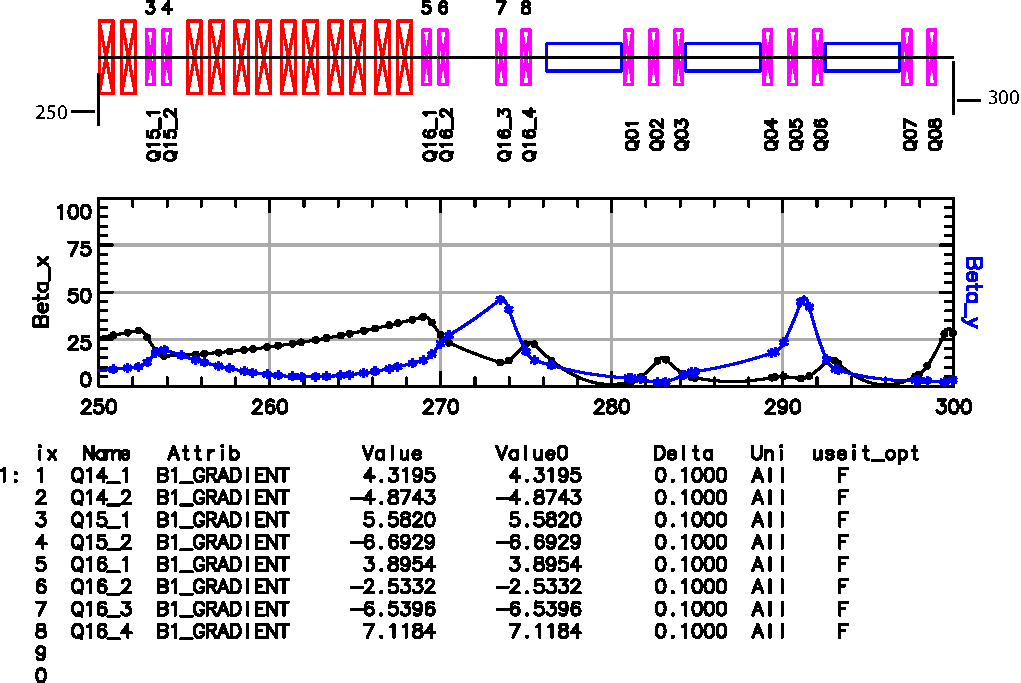
\includegraphics[width=5in]{layout-graph-table.pdf}
  \caption[Example key table with a lattice layout and data plots.]
{A lattice layout plot (top) above a data plot (middle) 
which in turn is above a key table plot (bottom). The points on the
curves in the data plot mark the edges of the elements displayed in
the lattice layout. Elements that have attributes that are varied as
shown in the key table have the corresponding key table number printed
above the element's glyph in the lattice layout.}
  \label{f:key.table}
\end{figure}

%% keys ------------------------------------------------------------------------
\section{List of Key Strokes}\index{single mode!list of Key strokes}
\label{s:keys}

In the following list, certain commands use multiple key strokes. For
example, the \vn{"/v"} command is invoked by first pressing the slash
(\vn{"/"}) key followed by the \vn{"v"} key. \vn{"a $<$left_arrow$>$"}
represents pressing the \vn{"a"} key followed by the left-arrow key.

Additionally, custom commands can be associated with any key using the
\vn{set key} command \sref{s:set}.

\begin{description}
\item[?]
Type a short help message.

\item[a $<$left\_arrow$>$]
Pan plots left by half the plot width.

\item[a $<$right\_arrow$>$]
Pan plots right by half the plot width.

\item[a $<$up\_arrow$>$]
Pan plots up by half the plot height.

\item[a $<$down\_arrow$>$]
Pan plots down by half the plot height.

\item[s $<$left\_arrow$>$]
Scale x-axis of plots by a factor of 2.0.

\item[s $<$right\_arrow$>$]
Scale x-axis of plots by a factor of 0.5

\item[s $<$up\_arrow$>$]
Scale y-axis of plots by a factor of 2.0.

\item[s $<$down\_arrow$>$]
Scale y-axis of plots by a factor of 0.5


\item[z $<$left\_arrow$>$]
Zoom x-axis of plots by a factor of 2.0.

\item[z $<$right\_arrow$>$]
Zoom x-axis of plots by a factor of 0.5

\item[z $<$up\_arrow$>$]
Zoom y-axis of plots by a factor of 2.0.

\item[z $<$down\_arrow$>$]
Zoom y-axis of plots by a factor of 0.5

\item[c]  
Show constraints.

\item[g]
Go run the default optimizer (\sref{s:tao.opti}). The optimizer will
run until you type a '.' (a period).  Periodically during the
optimization the variable values will be written to files, one for
each universe, whose name is \vn{tao_opt_vars\#.dat}. where \vn{\#} is
the universe number.

\item[v]
Show Bmad variable values in bmad lattice format. See also the
\vn{/v} command. Equivalent to \vn{show vars -bmad} in line mode.

\item[V] 
Same an \vn{v} except only variables currently enabled for optimization are shown.
This is equivalent to \vn{show vars -bmad -good} in line mode.

\item[Z] 
Go back to \vn{line mode}

\item[$<$]
Reduce the deltas (the amount that a variable is changed when you use
the keys 0 through 9) of all the variables by a factor of 2.

\item[$>$]
Increase the deltas (the amount that a variable is changed when you
use the keys 0 through 9) of all the variables by a factor of 2.

\item[$<$left\_arrow$>$]
Shift the active key bank down by 1: ib -$>$ ib - 1

\item[$<$right\_arrow$>$]
Shift the active key bank up by 1: ib -$>$ ib + 1

\item[/$<$up\_arrow$>$]
Increase all key deltas by a factor of 10.

\item[/$<$down\_arrow$>$]
Decrease all key deltas by a factor of 10.

\item[$<$CR$>$]
Do nothing but replot.

\item[-p]
Toggle plotting. Whether to plot or not to plot is initially
determined by \vn{plot%enable}.

\item['$<$command$>$]
Accept a Line Mode (\sref{c:command}) command.

\item[/b]
Switch the default lattice branch (\sref{s:lattice}).

\item[/e $<$Index or Name$>$]
Prints info on a lattice element. If there are two lattices being used
and only the information of an element from one particular lattice is
wanted then prepend with "n@" where n is the lattice index.

\item[/l]
Print a list of the lattice elements with Twiss parameters.

\item[/u $<$Universe Index$>$]
Switch the default universe (\sref{s:universe}).

\item[/v]
Write variable values to the default output file in Bmad lattice format. 
The default output file name is set by \vn{global%var_out}. 
See also the \vn{V} command.

\item[/x $<$min$>$ $<$max$>$]
Set the horizontal scale min and max values for all the plots. This is
the same as setting \vn{plot%x%min} and \vn{plot%x%max} in the \tao
input file. If \vn{min} and \vn{max} are not given then the scale will
be chosen to include the entire lattice.

\item[/y $<$min$>$ $<$max$>$]
Set the y-axis min and max values for all the plots. This is the same
as setting \vn{plot%y%min} and \vn{plot%y%max} in the \tao input
file. If \vn{min} and \vn{max} are not given then an autoscale will be
done.

\item[=v $<$digit$>$ $<$value$>$]
Set variable value. \vn{<digit>} is between 0 and 9 corresponding to a
variable of the current bank. \vn{<value>} is the value to set the
variable to.

\item[=$<$right\_arrow$>$]
Set saved ("value0") values to variable values to saved values. The
saved values (the value0 column in the display) are initially set to
the initial value on startup. There are saved values for both the
manual and automatic variables. Note that reading in a TOAD input file
will reset the saved values. If you want to save the values of the
variables in this case use "/w" to save to a file. Use the
"\vn{/$<$left_arrow$>$}" command to go in the reverse direction.

\item[=$<$left\_arrow$>$]
Paste saved (\vn{value0} column in the display) 
values back to the variable values.  The saved
values are initially set to the
initial value on startup. Use the "\vn{/$<$right_arrow$>$}" command to go in
the reverse direction.

\end{description}

\chapter{Python/GUI Interface}
\index{python interface}
\label{c:python}

%--------------------------------------------------------------------------
\section{Python Interface Via Pexpect}

A python module, \vn{tao_pipe.py}, for interfacing \tao to \vn{Python}
is provided in the \vn{tao/python} directory. 

The \vn{tao_pipe} module uses the \vn{pexpect} module. The
\vn{pexpect} module is a general purpose tool for interfacing
Python with programs like \tao. If \vn{pexpect} is not present
your system, it can be downloaded from
\vn{http://www.noah.org/wiki/pexpect}. 

Example:
\begin{example}
  >>> import tao_pipe                                       # import module
  >>> p = tao_pipe.tao_io("../bin/tao -lat my_lat.bmad")    # init session
  >>> p.cmd_in("show global")               # Command to Tao
  >>> print(p.output)                       # print the output from Tao
  >>> p.cmd("show global")                  # Like p.cmd_in() excepts prints the output too.
\end{example}

After each call to \vn{tao_io.cmd} and \vn{tao_io.cmd_in}, the
\vn{tao_io.output} variable is set to the multiline output string
returned by \tao. To chop this string into lines, use the splitlines()
string method.

\index{python}
To get information from \tao into Python, the output from \tao,
contained in \vn{tao_io.output}, needs to be parsed. For long term
maintainability of python scripts, use the \vn{python} (\sref{s:python}) command 
as opposed to the \vn{show} command . See the \vn{python} command for more details.

%--------------------------------------------------------------------------
\section{Tao Python command}




%--------------------------------------------------------------------------
\section{Plotting Issues}
\label{s:gui.plot}

When using \tao with a \vn{gui}, and when the \vn{gui} is doing the plotting, the \vn{-noplot}
option (\sref{s:command.line}) should be used when starting \tao. The \vn{-noplot} option prevents
\tao from opening a plotting window.

Even though \tao is not displaying the plot page when the \vn{-noplot} option is used, \tao will
still calculate the points needed for plotting curves for use by the \vn{gui}. In this case, a few
points must be kept in mind: First the names of the default plot regions are simplified to be 'r1',
'r2', etc. Use the \vn{show plot} command (\sref{s:show.plot}) to view a list. Second, to prevent
unneeded computation, the \vn{visible} parameter of template plots that are placed (\sref{s:place})
is set to False and must be set to True, using the \vn{set plot} command (\sref{s:set.plot}), to
enable computation of the curve points.


%----------------------------------------------------------------
\part{Programmer's Guide}

\chapter{Bmad Programming Overview}
\label{c:programming}

%-----------------------------------------------------------------------------
\section{Manual Notation}
\label{s:component}

\bmad defines a number of structures and these structures may contain
components which are structures, etc. In order to keep the text in
this manual succinct when referring to components, the enclosing
structure name may be dropped. For example, the \vn{lat_struct}
structure looks like
\begin{example}
  type lat_struct
    character(40) name               
    type (mode_info_struct) a, b, z  
    type (lat_param_struct) param    
    type (ele_struct), pointer ::  ele(:)
    type (branch_struct), allocatable :: branch(:)  
    ... etc. ...
  end type
\end{example}
In this example, ``\vn{%a}'' could be used to refer to, the \vn{a}
component of the \vn{lat_struct}.  To make it explicit that this is a
component of a \vn{lat_struct}, ``\vn{lat_struct%a}'' is an alternate
possibility. Since the vast majority of structures have the
``_struct'' suffix, this may be shortened to ``\vn{lat%a}''. A similar
notation works for subcomponents. For example, a \vn{branch_struct}
looks like
\begin{example}
  type branch_struct
    character(40) name
    integer ix_from_ele                  ! Index of branching element
    integer, pointer :: n_ele_track      ! Number of tracking elements
    integer, pointer :: n_ele_max
    type (ele_struct), pointer :: ele(:) ! Element array
    ... etc. ...
  end type
\end{example}
The \vn{ele} component of the \vn{branch} component of the
\vn{lat_struct} can be referred to using ``\vn{lat%branch%ele}'',
``\vn{%branch%ele}'', or ``\vn{%ele}''. Potentially, the last of these
could be confused with the ``\vn{lat%ele}'' component so ``\vn{%ele}''
would only be used if the meaning is unambiguous in the context.
%-----------------------------------------------------------------------
\section {The Bmad Libraries}
\label{s:libs}
\index{Bmad!distribution}

The code that goes into a program based upon \bmad is divided up into
a number of libraries. The \bmad web site has general information on
the organization of these libraries including information on obtaining
and compiling programs. The \bmad web site is at:
\begin{example}
    http://www.lepp.cornell.edu/~dcs/bmad
\end{example}

The \bmad libraries are divided into two groups. One group of
libraries contains the Cornell developed code. The other
\vn{``package''} libraries consist of non-Cornell code that \bmad
relies upon.

The Cornell developed code can further be divided into CESR storage
ring specific code and non-CESR specific code. The CESR specific code
will not be discussed in this Manual.

The Cornell developed non-CESR specific code libraries are:
subsidiary libraries are: 
\begin{description}
  \index{sim_utils library}
  \item[bmad] \Newline
The \vn{bmad} library contains the routines for relativistic charged
particle simulation including particle tracking, Twiss calculations,
symplectic integration, etc., etc.
  \item[cpp_bmad_interface]
The \vn{cpp_bmad_interface} library is for interfacing \bmad with C++.  This library
defines a set of C++ classes corresponding to the major \bmad structures. Along
with this, the library contains conversion routines to move information between 
the C++ classes and the corresponding \bmad structures.
  \item[sim_utils] \Newline
The \vn{sim_utils} library contains a set of miscellaneous helper routines. 
Included are routines for string manipulation, file manipulation,
matrix manipulation, spline fitting, Gaussian random number generation, etc. 
\end{description}

The \vn{package} libraries are:
\begin{description}
  \index{PTC/FPP!library}
  \item[forest] \Newline
This is the PTC/FPP (Polymorphic Tracking Code / Fully Polymorphic
Package) library of \'Etienne Forest that handles Taylor maps to any
arbitrary order (this is also known as Truncated Power Series Algebra
(TPSA)). See Chapter~\ref{c:ptc} for more details.  FPP/PTC is a
very general package and \bmad only makes use of a small part of its
features.  For more inform
ation see the FPP/PTC
manual\cite{b:ptc}. The core Differential Algebra (DA) package used
by PTC was developed by Martin Berz\cite{b:berz}.
  \index{fftw!library}
  \item[fftw] \Newline
FFTW is a C subroutine library for computing the discrete Fourier
transform in one or more dimensions. FFTW has a Fortran 2003 API.
  \index{gsl!library}
  \index{fgsl!library}
  \item[gsl / fgsl] \Newline
The Gnu Scientific Library (GSL), written in C, provides a wide range of mathematical
routines such as random number generators, special functions and least-squares
fitting. There are over 1000 functions in total. The FGSL library provides a Fortran
interface to the GSL library.
  \index{hdf5!library}
  \item[hdf5] \Newline
\vn{hdf5} is a library for for storing and managing data.
  \index{h5hut!library}
  \item[h5hut] \Newline
\vn{h5hut} is a library, based on \vn{hdf5} for storing particle data. Additionally,
there are associated programs for viewing the particle data.
  \index{lapack!library}
  \index{lapack95!library}
  \item[lapack / lapack95] \Newline
\vn{lapack} is a widely used package of linear algebra routines written in Fortran77. The
\vn{lapack95} library provides a Fortran95 interface to \vn{lapack}.
  \index{pgplot!library}
  \item[PGPLOT] \Newline
The \vn{pgplot} Graphics Subroutine Library is a Fortran or
C-callable, device-independent graphics package for making simple
scientific graphs. Documentation including a user's manual may be
obtained from the \vn{pgplot} web site at
\begin{verbatim}
    http://www.astro.caltech.edu/~tjp/pgplot.
\end{verbatim} 
One disadvantage of \vn{pgplot} for the programmer is that it is not the
most user friendly. To remedy this, there is a set of Fortran90
wrapper subroutines called \vn{quick_plot}.  The \vn{quick_plot}
suite is part of the \vn{sim_utils} library and is documented in
Chapter~\ref{c:quick.plot}.
  \index{plplot!library}
  \item[plplot] \Newline
The \vn{plplot} library is an updated version of \vn{pgplot}. The \vn{plplot}
library can be used as a replacement for \vn{pgplot}. The \vn{quick_plot}
suite, which is part of the \vn{sim_utils} library and is documented in
Chapter~\ref{c:quick.plot}, provides wrapper routines for \vn{plplot} to
make things more programmer friendly.
  \index{numerical recipes!library}
  \item[recipes] \Newline
Numerical Recipes is a set of subroutines for doing scientific
computing including Runge--Kutta integration, FFTs, interpolation and
extrapolation, etc., etc. The documentation for this library is the
books ``Numerical Recipes, in Fortran, The Art of Scientific
Computing'' and ``Numerical Recipes in Fortran90, the Art of Parallel
Scientific Computing''\cite{b:nr}.  The first book explains how the
subroutines work and the second book explains what the argument lists
for the Fortran90 version of the subroutines are. You do need both
books if you want to use Numerical Recipes. For \bmad, this library
has been modified to handle double precision reals which is the
standard for the other libraries (See \sref{s:precision}).
  \index{xraylib!library}
  \item[xraylib] \Newline
The XRAYLIB library provides routines for obtaining parameters
pertinent to the X-ray interaction with matter.
  \index{xsif!library}
  \item[xsif] \Newline
\vn{xsif} is a library from \vn{SLAC} to read in \vn{xsif} format files. See 
\sref{s:lattice.file.formats} for more details. The only
\bmad routine to use this library is \vn{xsif_parser}.
\end{description}

%-----------------------------------------------------------------------------
\section{Using getf and listf for Viewing Routine and Structure Documentation}
\label{s:getf}
\index{getf}
\index{listf}

As can be seen from the program example in Chapter~\ref{c:program.info}
there is a lot going on behind the scenes even for this
simple program. This shows that programming with \bmad can be both easy
and hard. Easy in the sense that a lot can be done with just a few
lines. The hard part comes about since there are many details that
have to be kept in mind in order to make sure that the subroutines
are calculating what you really want them to calculate.

To help with the details, all \bmad subroutines have in their source (.f90)
files a comment block that explains the arguments needed by the
subroutines and explains what the subroutine does. To help quickly
access these comments, there are two Perl scripts that are supplied
with the \bmad distribution that are invoked with the commands
\vn{listf} and \vn{getf}.

The \vn{getf} command is used to locate routines and structures, and
to type out information on them.  The form of the command is
\begin{verbatim}
    getf <name>
\end{verbatim}
This searches for any routine or structure with the name
\vn{<name>}. \vn{<name>} may contain the wild--cards ``*'' and ``.'' where
``*'' matches to any number of characters and ``.'' matches to any
single character. For example:
\begin{example}
    getf bmad_parser
    getf lat_struct
    getf twiss_at_.
\end{example}
The third line in this example will match to the routine
\vn{twiss_at_s} but not the routine \vn{twiss_at_start}. You may or
may not have to put quotation marks if you use wild card characters.
As an example, the command \vn{getf twiss_struct} produces:
\begin{example}
  /home/cesrulib/cesr_libs/devel/cvssrc/bmad/modules/twiss_mod.f90
    type twiss_struct
      real(rp) beta, alpha, gamma, phi, eta, etap
      real(rp) sigma, emit
    end type
\end{example}
The first line shows the file where the structure is located (This is
system and user dependent so don't be surprised if you get a different
directory when you use \vn{getf}). The rest of the output shows the
definition of the \vn{twiss_struct} structure.  The result of issuing
the command \vn{getf relative_tracking_charge} is:
\begin{example}
  File: ../../bmad/modules/bmad_utils_mod.f90
  !+
  ! Function relative_tracking_charge (orbit, param) result (rel_charge)
  !
  ! Routine to determine the relative charge/mass of the particle being
  ! tracked relative to the charge of the reference particle.
  !
  ! Input:
  !   orbit -- coord_struct: Particle position structure.
  !   param -- lat_param_struct: Structure holding the reference particle id.
  !
  ! Output:
  !   rel_charge -- real(rp): Relative charge/mass
  !-
  function relative_tracking_charge (orbit, param) result (rel_charge)
\end{example}
The first line again shows in what file the subroutine is located.
The rest of the output explains what the routine does and how it
can be called.

The \vn{listf} command is like the \vn{getf} command except that only
the file name where a routine or structure is found is printed.
The \vn{listf} command is useful if you
want to just find out where a routine or structure definition lives.
For example, the \vn{listf relative*} command would produce
\begin{example}
  File: ../../bmad/code/relative_mode_flip.f90
      function relative_mode_flip (ele1, ele2) result (rel_mode)

  File: ../../bmad/modules/bmad_utils_mod.f90
      function relative_tracking_charge (orbit, param) result (rel_charge)
\end{example}

The way \vn{getf} and \vn{listf} work is that they search a list of
directories to find the \vn{bmad}, \vn{sim_utils}, and \vn{tao}
libraries. Currently the libraries in the \bmad distribution that were
not developed at Cornell are not searched. This is primarily due to
the fact that, to save time, \vn{getf} and \vn{listf} make assumptions
about how documentation is arranged in a file and the non--Cornell libraries 
do not follow this format.

%-----------------------------------------------------------------------
\section{Precision of Real Variables}
\label{s:precision}
\index{programming!precision (rp)}
\index{rp}


Historically, \bmad come in two flavors: One version where the real
numbers are single precision and a second version with double
precision reals. Which version you are working with is controlled by
the kind parameter \vn{rp}\ (Real Precision) which is defined in the
\vn{precision_def} module. On most platforms, single precision
translates to \vn{rp}\ = 4 and double precision to \vn{rp}\ = 8. The
double precision version is used by default since round-off errors can
be significant in some calculations. Long--term tracking is an example
where the single precision version is not adequate. Changing the
precision means recompiling all the libraries except \vn{PTC} and
\vn{pgplot}.  You cannot mix and match. Either you are using the
single precision version or you are using the double precision
version. Currently, \bmad is always compiled double precision and it
is a near certainty that there would have to be some fixes if there
was ever a need for compiling single precision.

To define floating point variables in Fortran with the correct precision,
 use the syntax {\tt ``real(rp)''}. For example:
\begin{example}
    real(rp) var1, var2, var3
\end{example}
When you want to define a literal constant, for example to pass an
argument to a subroutine, add the suffix \vn{_rp} to the end of the
constant. For example
\begin{example}
   var1 =  2.0_rp * var2
   call my_sub (var1, 1.0e6_rp)
\end{example}
Note that \vn{2_rp} is different from \vn{2.0_rp}. \vn{2_rp} is an
integer of kind \vn{rp}, not a real.

Independent of the setting of \vn{rp}, the parameters \vn{sp} and
\vn{dp} are defined to give single and double precision numbers
respectively.

%-----------------------------------------------------------------------------
\section{Programming Conventions}
\index{programming!conventions}

\bmad subroutines follow the following conventions:

\begin{description}

\index{\$!character to denote a parameter}
\item[A ``\$'' suffix denotes a parameter:] 
A ``\$'' at the end of a name denotes an 
integer parameter. For example, in the above program, to check
whether an element is a quadrupole one would write:
\begin{verbatim}
  if (lat%ele(i)%key == quadrupole$) ...
\end{verbatim}
Checking the source code one would find in the module \vn{bmad_struct}
\begin{verbatim}
  integer, parameter :: drift$ = 1, sbend$ = 2, quadrupole$ = 3, group$ = 4
\end{verbatim}
One should always use the parameter name instead of the integer it represents.
That is, one should never write
\begin{verbatim}
  if (lat%ele(i)%key == 3) ...  ! DO NOT DO THIS!
\end{verbatim}
For one, using the name makes the code clearer. However, more
importantly, the integer value of the parameters may at times be
shuffled for practical internal reasons. The use of the integer value
could thus lead to disastrous results.  

\index{structures}
\item[Structure names have a ``_struct'' suffix:]
For example: \vn{lat_struct}, \vn{ele_struct}, etc. Structures without a 
\vn{_struct} are usually part of \'Etienne's PTC/FPP package.

\end{description}

%-----------------------------------------------------------------------
%\section {Using Modules}
%\label{s:modules}
%\index{modules}



\chapter{Customizing Tao}
\index{customizing}
\label{c:custom.tao}

\tao has been designed to be readily extensible with a minimum of
effort when certain rules are followed. 
This chapter discusses how this is done.

%----------------------------------------------------------------
\section{Initial Setup}
\label{s:cust.init}

Creating a custom version of \tao involves creating custom code that is put in a directory that is
distinct from the \vn{tao} directory that contains the standard \tao code files.

\textbf{It is important to remember that the code in the \vn{tao} directory is not to be modified.
This ensures that, as time goes on, and as \tao is developed by the "Taoist" developers, changes to
the code in the \vn{tao} directories will have a minimal chance to break your custom code.} If you do
feel you need to change something in the \vn{tao} directory, please seek help first.

To setup a custom \tao version do the following:
  \begin{enumerate}
  \item
Establish a base directory in which things will be built. This directory can have any name. Here we
will call this directory \vn{ROOT}.
  \item
Make a subdirectory of \vn{ROOT} that will contain the custom code.  This directory can have any
name.  Here this directory will be called \vn{tao_custom}.
  \item
Copy the files from the directory \vn{tao/customization} to \vn{ROOT/tao_custom}. The \vn{tao}
directory is part of the \bmad package. If you do not know where to find it, ask your local Guru
where it is. Along with a \vn{README} file, there are two CMake\footnote{CMake is a program used for
compiling code}  script files in the
\vn{customization} directory:
\begin{example}
  CMakeLists.txt
  cmake.custom_tao
\end{example}
These scripts are setup to make an executable called \vn{custom_tao}. This name can be changed
by modifying the \vn{cmake.custom_tao} file.
  \item
Copy the file \vn{tao/program/tao_program.f90} to \vn{ROOT/tao_custom}.
  \item
Copy as needed \vn{hook} files from \vn{tao/hook} to \vn{ROOT/tao_custom}. The hook files
you will need are the hook files you will want to modify to customize \tao. See below for
details. See \sref{s:cust.example} for an example.
  \item
Go to the \vn{ROOT/tao_custom} directory and use the command \vn{mk} to create the
executable 
\begin{example}
    \vn{ROOT/production/bin/custom_tao}. 
\end{example}
Similarly, the command \vn{mkd} will create a debug executable 
\begin{example}
    \vn{ROOT/debug/bin/custom_tao}
\end{example}
	\end{enumerate}
A debug executable only needs to be created if you a debugging the code.

%----------------------------------------------------------------
\section{It's All a Matter of Hooks}
\index{customizing!hooks}

The golden rule when extending \tao is that you are only allowed to
customize routines that have the name ``hook'' in
them. These files are located in the directory \vn{tao/hook}.
To customize one of these files, copy it from \vn{tao/hook} to \vn{ROOT}
and then make modifications to the copy.

The reason for this golden rule is to ensure that, as time
goes by, and revisions are made to the \tao routines to extend it's
usefulness and to eliminate bugs, these changes will
have a minimum impact on the specialized routines you write.
What happens if the modification you want to do cannot be accomplished
by customizing a hook routine? The answer is to contact
the \tao programming team and we will modify \tao and provide the hooks 
you need so that you can then do your customization.

%----------------------------------------------------------------
\section{Initializing Hook Routines}

One way to initialize a hook routine is to read in parameters from an initialization file.
If an initialization file is used, the filename may be set using the
\vn{s%global%hook_init_file} string. This string may be set in the \vn{tao_params}
namelist (\sref{s:globals} or may be set on the command line using the
\vn{-hook_init_file} option (\sref{s:command.line}).

%----------------------------------------------------------------
\section{Hook Routines}

To get a good idea of how \tao works it is recommended to spend a
little bit of time going through the source files. This may also
provide pointers on how to make customizations in the hook routines. Of
particular interest is the module \vn{tao_lattice_calc_mod.f90} where tracking
and lattice parameters are computed. 

Plotting is based upon the \vn{quick_plot} subroutines which are
documented in the \bmad reference manual. If custom plotting is
desired this material should be reviewed to get familiar with the
concepts of ``graph'', ``box'', and ``page''.

The following is a run through of each of the hook routines. Each
routine is in a separate file called
\vn{tao/hook/<hook_routine_name>.f90}. See these files for subroutine
headers and plenty of comments throughout the dummy code to aid in the
modification of these subroutines.

%-----------------------------------------------------------------
\subsection{tao_hook_graph_setup}
\index{customizing!tao_hook_graph_data_setup}

Use this to setup custom graph data for a plot.

%-----------------------------------------------------------------
\subsection{tao_hook_command}\index{customizing!tao_hook_commad}
\label{s:hook.command}

Any custom commands are placed here. The dummy subroutine already has
a bit of code that replicates what is performed in
\vn{tao_command}. Commands placed here are searched before the
standard \tao commands. This allows for the overwriting of any
standard \tao command.

By default, there is one command included in here: \vn{`hook'}. This
is just a simple command that doesn't really do anything and is for
the purposes of demonstrating how a custom command would be
implemented.

The only thing needed to be called at the end of a custom command is
\vn{tao_cmd_end_calc}. This will perform all of the steps listed in
Section~\sref{s:lat.calc}.

See Sec.~\sref{s:cust.read.example} for an example of how to use this hook.

%-----------------------------------------------------------------
\subsection{tao_hook_evaluate_a_datum}
\index{customizing!tao_hook_evaluate_a_datum}

Any custom data types are defined and calculated here. If a non-standard data type is listed in the
initialization files, then a corresponding data type must be placed in this routine. The tutorial
uses this hook routine when calculating the emittance.

Dependent lattice parameters (such as closed orbits, beta functions, etc.) are recalculated every
time \tao believes the lattice has changed (for example, after a \vn{change} command).  This is done
in \vn{tao_lattice_calc}. \vn{tao_lattice_calc} in turn calls \vn{tao_evaluate_a_datum} for each
datum. \vn{tao_evaluate_a_datum} in turn calls \vn{tao_hook_evaluate_a_datum} to allow for custom
data evaluations. 

See the \vn{tao_evaluate_a_datum} routine as an example as how to handle datums.
The arguments for \vn{tao_hook_evaluate_a_datum} is
\begin{example}
  tao_hook_evaluate_a_datum (found, datum, u, tao_lat, datum_value, valid_value)
\end{example}
The \vn{found} logical argument should be set to \vn{True} for datums that are handled by this
hook routine and \vn{found} sould be set to \vn{False} for all other datums.

%-----------------------------------------------------------------
\subsection{tao_hook_init1 and tao_hook_init2}
\label{s:hook.init}
\index{customizing!tao_hook_init}

After the \vn{design} lattice and the global and universe structures are initialized,
\vn{tao_hook_init1} is called from the \vn{tao_init} routine. Here, any further
initializations can be added. In particular, if any custom hook structures need to be
initialized, here's the place to do it. 

Further down in \vn{tao_init}, \vn{tao_hook_init2} is called. Normally you will want to
use \vn{tao_hook_init1}. However, \vn{tao_hook_init2} can be used, for example, ! to set
model variable values different from design variable values since when \vn{tao_hook_init1}
is called the \vn{model} lattice has not yet been initialized.

%-----------------------------------------------------------------
\subsection{tao_hook_init_design_lattice}
\index{customizing!tao_hook_init_design_lattice}

This will do a custom lattice initialization. The standard lattice
initialization just calls \vn{bmad_parser} or \vn{xsif_parser}. If
anything more complex needs to be done then do it here. This is also
where any custom overlays or other elements would be inserted after
the parsing is complete. But in general, anything placed here should,
in principle, be something that can be placed in a lattice file.

\textbf{This is the only routine that should insert elements in the
ring}. This is because the \tao data structures use the element index
for each element associated with the datum. If all the element indexes
shift then the data structures will break. If new elements need to be
inserted then modify this routine and recompile. You can alternatively
create a custom initialization file used by this routine that reads in
any elements to be inserted.

%-----------------------------------------------------------------
\subsection{tao_hook_lattice_calc}
\index{customizing!tao_hook_lattice_calc}

The standard lattice calculation can be performed for single particle,
particle beam tracking and will recalculate the
orbit, transfer matrices, twiss parameters and load the data
arrays. If something else needs to be performed whenever the lattice
is recalculated then it is placed here. A custom lattice calculation
can be performed on any lattice separately, this allows for the
possibility of, for example, tracking a single particle for one
lattice and beams in another.

%-----------------------------------------------------------------
\subsection{tao_hook_merit_data}
\index{customizing!tao_hook_merit_data}

A custom data merit type can be defined here. Table~\ref{t:con.type}
lists the standard merit types. If a custom merit type is used then
\vn{load_it} in \vn{tao_hook_load_data_array} may also need to be
modified to handle this merit type, additionally, all standard data
types may need to be overridden in \vn{tao_hook_load_data_array} in
order for the custom \vn{load_it} to be used.  See
\vn{tao_merit.f90} for how the standard merit types are
calculated.

%-----------------------------------------------------------------
\subsection{tao_hook_merit_var}
\index{customizing!tao_hook_merit_var}

This hook will allow for a custom variable merit type. However, since
there is no corresponding data transfer, no \vn{load_it} routine needs
to be modified.  See \vn{tao_merit.f90} for how the standard
merit types are calculated.

%-----------------------------------------------------------------
\subsection{tao_hook_optimizer}
\index{customizing!tao_hook_optimizer}

If a non standard optimizer is needed, then it can be implemented
here. See the \vn{tao_*_optimizer.f90} files for how the
standard optimizers are implemented.

%-----------------------------------------------------------------
\subsection{tao_hook_plot_graph}
\index{customizing!tao_hook_plot_graph}

This will customize the plotting of a graph. See the \tao module
\vn{tao_plot_mod} for details on what it normally done. You will also
need to know how \vn{quick_plot} works (See the \bmad manual).

%-----------------------------------------------------------------
\subsection{tao_hook_plot_data_setup}
\index{customizing!tao_hook_plot_data_setup}

Use this routine to override the \vn{tao_plot_data_setup} routine which
essentially transfers the information from the \vn{s%u(:)%data} arrays
to the \vn{s%plot_page%region(:)%plot%graph(:)%curve(:)} arrays. This
may be useful if you want to make a plot that isn't simply the
information in a data or variable array.

%-----------------------------------------------------------------
\subsection{tao_hook_post_process_data}
\index{customizing!tao_hook_post_process_data}

Here can be placed anything that needs to be done after the data
arrays are loaded. This routine is called immediately after the data
arrays are called and before the optimizer or plotting is done, so any
final modifications to the lattice or data can be performed here.

%-----------------------------------------------------------------
%\chapter{Plotting}
%\label{s:prog.plotting} 

%\fbox{this chapter is yet to be completed!} 

%----------------------------------------------------------------
\section{Adding a New Data Type Example}
\label{s:cust.example}

As an example of a customization, let's include a new data type called
\vn{particle_emittance}. This will be the non-normalized x and y
emittance as found from the Courant-Snyder invariant. This data type
will behave just like any other data type (i.e.  \vn{orbit},
\vn{phase} etc...). 

This example will only require the modification of one file:
\vn{tao_hook_evaluate_a_datum.f90}. This file should be copied
from the \vn{tao/hook} directory and put in your \vn{ROOT/code}
directory (\sref{s:cust.init}).

The formula for single particle emittance is
\Begineq
  \epsilon = \gamma x^{2} + 2 \alpha x x' + \beta x'^{2}
  \label{e:emittance}
\Endeq
Place the following code in \vn{tao_hook_evaluate_a_datum.f90} in the
\cmd{case select} construct (also add the necessary type declarations)
\begin{example}
  type (coord_struct), pointer :: orbit(:)
  ...
  orbit => tao_lat%tao_branch(0)%orbit
  ...
  case ('particle_emittance.x') 
    datum_value =  (ele%a%gamma * orbit(ix1)%vec(1)**2 + &
		     2 * ele%a%alpha * orbit(ix1)%vec(1) * orbit(ix1)%vec(2) + &
		     ele%a%beta * orbit(ix1)%vec(2)**2)
    
  case ('particle_emittance.y')
    datum_value = (ele%b%gamma * orbit(ix1)%vec(3)**2 + &
		     2 * ele%b%alpha * orbit(ix1)%vec(3) * orbit(ix1)%vec(4) + &
		     ele%b%beta * orbit(ix1)%vec(4)**2)
\end{example}
This defines what is to be calculated for each \vn{particle_emittance}
datum.  There are two transverse coordinates, so two definitions need
to be made, one for each dimension.

Now you just need to declare the data types in the \cmd{tao.init} and
\cmd{tao_plot.init} files. For the sake of this example, modify the
example files found in the \vn{tao/example} directory
\begin{example}
	mkdir ROOT/my_example
  cp tao/example/*.init ROOT/my_example
  cp tao/example/*.lat ROOT/my_example
\end{example}

In \cmd{ROOT/my_example/tao.init} add the following lines to the data
declarations section
\begin{example}
  &tao_d2_data
    d2_data%name = "particle_emittance" 
    universe = 0 
    n_d1_data = 2
  /

  &tao_d1_data
    ix_d1_data = 1
    d1_data%name = "x"  
    default_weight = 1
    use_same_lat_eles_as = 'orbit.x"
  /

  &tao_d1_data
    ix_d1_data = 2
    d1_data%name = "y"  
    default_weight = 1
    use_same_lat_eles_as = 'orbit.x"
  /
\end{example}

In \cmd{ROOT/my_example/tao_plot.init} add the following lines to the end
of the file
\begin{example}
  &tao_template_plot
    plot%name = 'particle_emittance'
    plot%x%min =   0
    plot%x%max = 100
    plot%x%major_div = 10
    plot%x%label = ' '
    plot%x_axis_type = 'index'
    plot%n_graph = 2
  /
  
  &tao_template_graph
    graph%name = 'x'
    graph_index = 1
    graph%box = 1, 2, 1, 2
    graph%title = 'Horizontal Emittance (microns)'
    graph%margin =  0.15, 0.06, 0.12, 0.12, '%BOX'
    graph%y%label = 'x'
    graph%y%max =  15
    graph%y%min =  0.0
    graph%y%major_div = 4
    graph%n_curve = 1
    curve(1)%data_source = 'data'
    curve(1)%data_type   = 'particle_emittance.x'
    curve(1)%y_axis_scale_factor = 1e6 !convert from meters to microns
  /

  &tao_template_graph
    graph%name = 'y'
    graph_index = 2
    graph%box = 1, 1, 1, 2
    graph%title = 'Vertical Emittance (microns)'
    graph%margin =  0.15, 0.06, 0.12, 0.12, '%BOX'
    graph%y%label = 'Y'
    graph%y%max =  15
    graph%y%min =  0.0
    graph%y%major_div = 4
    graph%n_curve = 1
    curve(1)%data_source = 'data'
    curve(1)%data_type = 'particle_emittance.y'
    curve(1)%units_factor = 1e6 !convert from meters to microns
  /
\end{example}
These namelists are described in detail in Chapter~\ref{c:init}.

We are now ready to compile and then run the program. The \tao library
should have already been created so all you need to do is
\begin{example}
	cd ROOT/code
	mk
  cd ROOT/my_example
  ../production/bin/custom_tao
\end{example}

After your custom \tao initializes type
\begin{example}
  place bottom particle_emittance
  scale
\end{example}
Your plot should look like Figure~\ref{f:plot.emittance}.

The emittance (as calculated) is not constant. This is due to
dispersion and coupling throughout the ring. \bmad provides a routine
to find the particle emittance from the twiss parameters that includes
dispersion and coupling called \vn{orbit_amplitude_calc}.

\begin{figure}
  \centering
  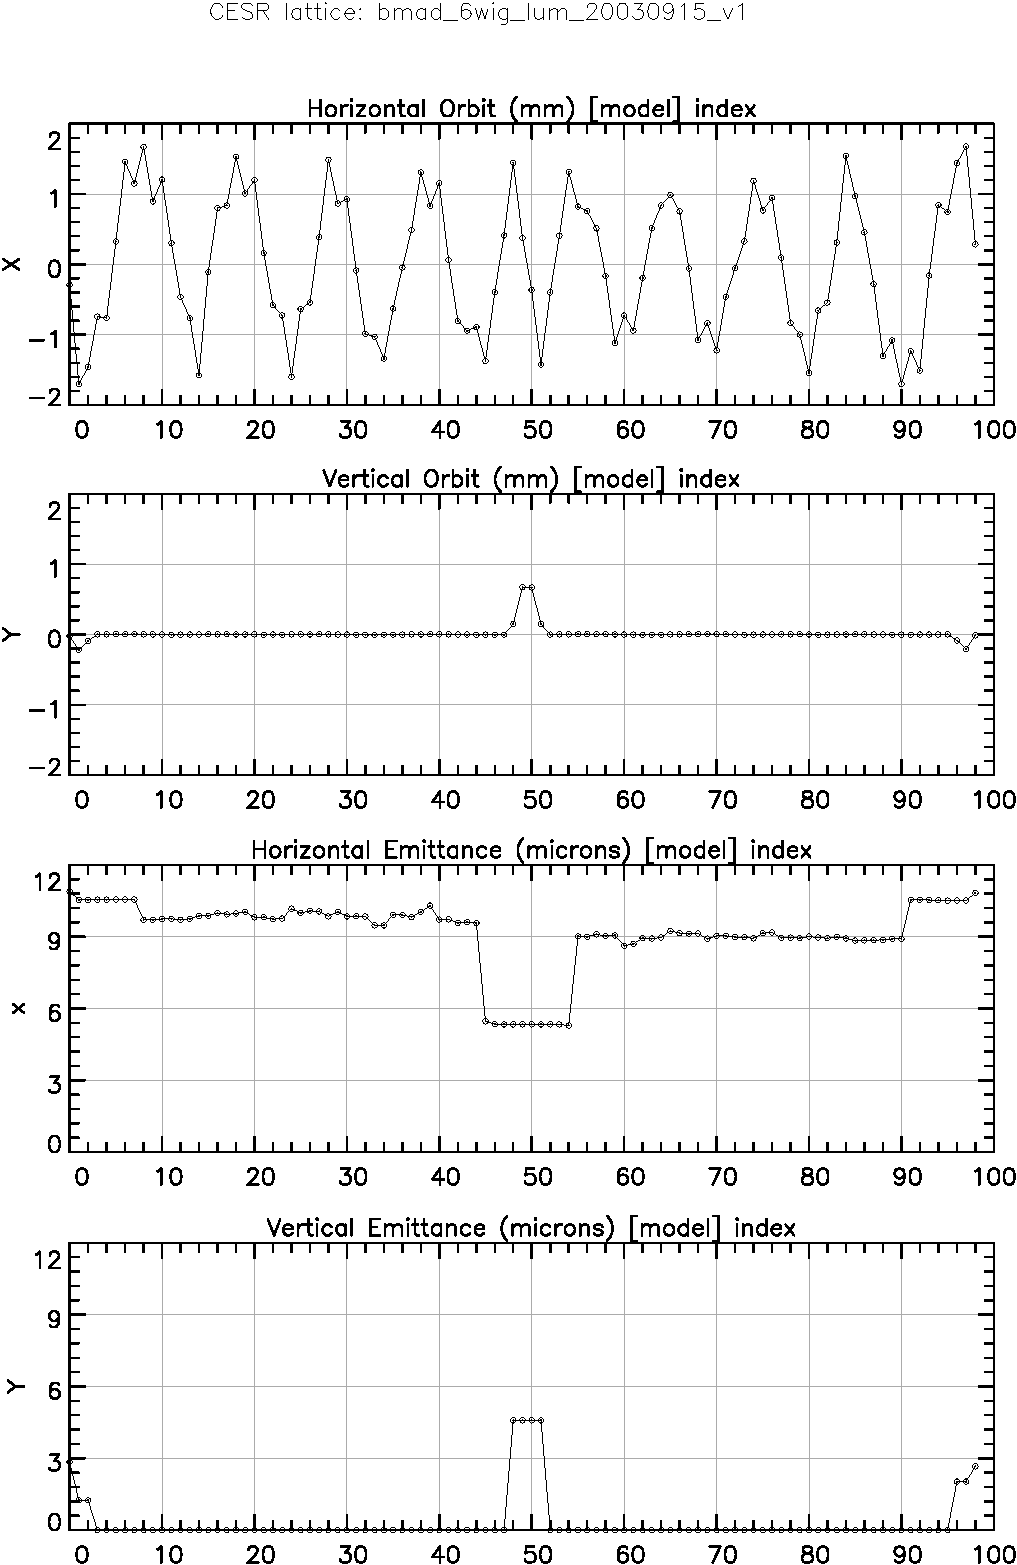
\includegraphics[width=5in]{plot-emittance.pdf}
  \caption{Custom data type: non-normalized emittance}
  \label{f:plot.emittance}
\end{figure}

%----------------------------------------------------------------
\section{Reading in Measured Data Example}
\label{s:cust.read.example}

This section shows how to construct a customized version of \tao, called \vn{ping_tao}, to
read in measured data for analysis. This example uses data from the Fermilab proton
recirculation. The data is obtained by measuring the orbit turn-by-turn of a beam that has been
initially pinged to give it a finite oscillation amplitude.

The files for constructing \vn{ping_tao} can be found
in the directory
\begin{example}
  tao/examples/custom_tao_with_measured_data
\end{example}
The files in this directory are as follows:
\begin{description}
  \item[CMakeLists.txt, cmake.ping_tao] \Newline
Script files for creating \vn{ping_tao}. See Sec.~\sref{s:cust.init}.
  \item[README] \Newline
The \vn{README} file gives some instructions on how to create \vn{ping_tao}
  \item[RRNOVAMU2E11172016.bmad] \Newline
Lattice file for the proton recirculation ring.
  \item[data] \Newline
Directory where some ping data is stored
  \item[tao.init] \Newline
\tao initialization file defining the appropriate data and variable structures (\sref{s:init.global})
  \item[tao.startup] \Newline
File with some command that are executed when \tao is started. These commands will read in
and plot some data.
  \item[tao_hook_command.f90] \Newline
Custom code for reading in ping data. The template used to construct this file is at
\vn{tao/hook/tao_hook_command.f90} (\sref{s:hook.command}).
  \item[tao_plot.init] \Newline
File for defining plot parameters (\sref{s:init.plot}).
  \item[tao_program.f90] \Newline
copy of the \vn{tao/program/tao_program.f90} file (\sref{s:cust.init}).
\end{description}

After creating the \vn{ping_tao} program (see the \vn{README} file), the program can
be run by going to the custom_tao_with_measured_data directory and using the command:
\begin{example}
	../production/bin/ping_tao
\end{example}

The customized \vn{tao_hook_command} routine implements a custom command called
\vn{pingread}.  This command will read in ping data. Ping data is the amplitude and phase
of the beam oscillations at a BPM for either the \vn{a-mode} or \vn{b-mode} oscillations.
See the write up on ping data types in Sec.~\sref{s:data.types} under \vn{ping_a.amp_x},
and \vn{ping_b.amp_x} for more details.

The data files in the \vn{data} directory contain data for either the \vn{a-mode} or \vn{b-mode} ping at either
the horizontal or vertical BPMs.

The syntax of the \vn{pingread} command is:
\begin{example}
  pingread <mode> <filename> <data_or_ref>
\end{example}
The first argument, \vn{<mode>}, should be either ``\vn{a_mode}'' ``\vn{b_mode}''
indicating wether the data is for the \vn{a-mode} \vn{b-mode} analysis (a better setup
would encode this information in the data file itself). The second argument, \vn{filename}
is the name of the data file, and the third argument, \vn{data_or_ref} should be
``\vn{data}'' or ``\vn{reference}'' indicating that the data is to be read into the
\vn{meas_value} or \vn{ref_value} of the appropriate \vn{tao_data_struct}.

%----------------------------------------------------------------
\subsection{Analysis of the tao_hook_command.f90 File}
\label{s:hook.cmd.anal}

The first part of the \vn{tao_hook_command} routine parses the command line to see
if the \vn{pingread} command is present. The relevant code, somewhat condensed, is:
\begin{example}
  subroutine tao_hook_command (command_line, found)

  !!!! put your list of hook commands in here. 

  character(16) :: cmd_names(1) = [character(16):: 'pingread']  

  ! "found" will be set to TRUE if the command is found.

  found = .false.

  ! strip the command line of comments

  call string_trim (command_line, cmd_line, ix_line)
  ix = index(cmd_line, '!')
  if (ix /= 0) cmd_line = cmd_line(:ix-1)        ! strip off comments

  ! blank line => nothing to do

  if (cmd_line(1:1) == '') return

  ! match first word to a command name
  ! If not found then found = .false.

  call match_word (cmd_line(:ix_line), cmd_names, ix_cmd, .true., .true., cmd_name)
  if (ix_cmd < 0) then
    call out_io (s_error$, r_name, 'AMBIGUOUS HOOK COMMAND')
    found = .true.
    return
  endif

  found = .true.
  call string_trim (cmd_line(ix_line+1:), cmd_line, ix_line)
\end{example}

Note: To quickly find information on routines and structures, use the \vn{getf} and \vn{listf}
scripts as explained in the \bmad manual. For example, typing ``\vn{getf string_trim}'' 
on the system command line will give information on the string_trim subroutine.

The above code tests to see if the command is \vn{pingread} and, if not, returns without
doing anything.

If the \vn{pingread} command is found, the rest of the command line is parsed to get the 
\vn{<mode>}, \vn{<filename>}, and \vn{<data_or_ref>} arguments.

In the \vn{tao.init} file, a \vn{tune} d2 datum is setup to have two \vn{d1} datum arrays
One for the \vn{a}-mode tune and one for the \vn{b}-mode tune:
\begin{example}
  \&tao_d2_data
    d2_data%name = "tune"
    universe = '*'  ! apply to all universes
    n_d1_data = 2
  /

  \&tao_d1_data
    ix_d1_data = 1
    d1_data%name = "a"
    default_weight = 1e6
    ix_min_data = 1
    ix_max_data = 1
  /

  \&tao_d1_data
    ix_d1_data = 2
    d1_data%name = "b"
    default_weight = 1e6
    ix_min_data = 1
    ix_max_data = 1
  /
\end{example}
And each \vn{d1} array has only one datum since the \vn{a}-mode and \vn{b}-mode tunes have
only one value associated with them (as opposed to, say an orbit which will have multiple
values from different BPMs).

In a data file there is a header section which, among other things, records the tune.
In a line beginning with the word ``\vn{Tune}''. Example:
\begin{example}
                   Horz         Vert         Sync.                           
   Tune           ( .452444)   ( .404434)   ( 0      ) 2p                    
\end{example}

In the \vn{tao_hook_command} file, after the arguments are parsed, the header part of the
data file is read to extract the tune datums:
\begin{example}
  type (tao_d2_data_array_struct), allocatable :: d2(:)
  ...
  if (line(1:4) == 'Tune') then
    call tao_find_data (err, 'tune', d2_array = d2)
    if (size(d2) /= 1) then
      call out_io (s_fatal$, r_name, 'NO TUNE D2 DATA STRUCTURE DEFINED!')
      return
    endif
\end{example}
The call to \vn{tao_find_data} looks for a \vn{d2} data structure named \vn{tune}. This
structure is setup in the \vn{tao.init} file. Alternatively, the \vn{ping_tao} program
could be configured to automatically setup the appropriate data and/or variable structures
via the \vn{tao_hook_init1} routine (\sref{s:hook.init}). 

The returned value from the call to \vn{tao_find_data} is an array called \vn{d2} of type
\vn{tao_d2_data_array_struct}. \vn{d2} holds an array of pointers to all
\vn{d2_data_struct} structures it can find. In general, there could be multiple such
structures if multiple universes are being used or if the match string, in this case
\vn{'tune'}, contained wild card characters. In this case, the expectation is that there
will only one universe used and thus there should be one and only one structure that
matches the name \vn{tune}. This structure will be pointed to by \vn{d2(1)%d2}. The
appropriate datums, will be:
\begin{example}
  d2(1)%d2%d1(1)%d(1)   ! a-mode tune
  d2(1)%d2%d1(1)%d(2)   ! b-mode tune
\end{example}
The values read from the data file are put in these datums via the code:
\begin{example}
  if (data_or_ref == 'data') then
    d2(1)%d2%d1(1)%d(1)%meas_value = twopi * (data_tune_a + nint(design_tune_a))
    d2(1)%d2%d1(1)%d(1)%good_meas = .true.
    d2(1)%d2%d1(2)%d(1)%meas_value = twopi * (data_tune_b + nint(design_tune_b))
    d2(1)%d2%d1(2)%d(1)%good_meas = .true.
  else
    d2(1)%d2%d1(1)%d(1)%ref_value = twopi * (data_tune_a + nint(design_tune_a))
    d2(1)%d2%d1(1)%d(1)%good_ref = .true.
    d2(1)%d2%d1(2)%d(1)%ref_value = twopi * (data_tune_b + nint(design_tune_b))
    d2(1)%d2%d1(2)%d(1)%good_ref = .true.
  endif      
\end{example}

The next step is to setup pointers to the appropriate data arrays to receive the ping data.
In the data file the ping data looks like:
\begin{example}
  BPM           Phase    Ampl.   RMSdev     Beta  bml_psi *Calib Old_Cal     
  R:HP222    -0.27314  0.46085    0.078    1.863  0.35183                         
  R:HP224    -0.05939  0.28277    0.143    0.701 -0.43442                         
  R:HP226     0.23140  0.31712    0.075    0.882 -0.14363                         
  ... etc ...
\end{example}
The ``\vn{H}'' in \vn{R:HP222}, etc. indicates that the data is from BPMs that only
measure the horizontal displacement of the beam. Alternatively, a ``\vn{V}'' would
indicate data from vertical measurement BPMs.

In the \vn{tao_hook_command} file the data pointers are setup by the code:
\begin{example}
  type (tao_d1_data_array_struct), allocatable, target :: d1_amp_arr(:), d1_phase_arr(:)
  ...
  if (line(3:3) == 'H') then
    if (mode == 'a_mode') then
      call tao_find_data (err, 'ping_a.amp_x', d1_array = d1_amp_arr)
      call tao_find_data (err, 'ping_a.phase_x', d1_array = d1_phase_arr)
    else 
      call tao_find_data (err, 'ping_b.amp_x', d1_array = d1_amp_arr)
      call tao_find_data (err, 'ping_b.phase_x', d1_array = d1_phase_arr)
    endif
  elseif (line(3:3) == 'V') then
    if (mode == 'a_mode') then
      call tao_find_data (err, 'ping_a.amp_y', d1_array = d1_amp_arr)
      call tao_find_data (err, 'ping_a.phase_y', d1_array = d1_phase_arr)
    else 
      call tao_find_data (err, 'ping_b.amp_y', d1_array = d1_amp_arr)
      call tao_find_data (err, 'ping_b.phase_y', d1_array = d1_phase_arr)
    endif
\end{example}
\vn{line(3:3)} is either \vn{H} or \vn{V} indicating horizontal or vertical orbit
measuring BPMs. In this case, the call to the \vn{tao_find_data} routine returns \vn{d1}
data arrays to the amplitude data (\vn{d1_amp_arr}) and phase data (\vn{d1_phase_arr}).
Just like the tune data, since it is assumed only one universe is being used, there should
be one and only \vn{d1} structure for the phase and only one \vn{d1} structure for the amplitude:
\begin{example}
  d1_amp_arr(1)%d1      ! d1 struucture for the amplitude data
  d1_phase_arr(1)%d1    ! d1 struucture for the phase data
\end{example}
To save on typing, and make the code clearer, pointers are used to point to these structures:
\begin{example}
  type (tao_d1_data_struct), pointer :: d1_phase, d1_amp
  ...
  d1_amp => d1_amp_arr(1)%d1
  d1_phase => d1_phase_arr(1)%d1
\end{example}
The array of datums for the amplitude and phase data will be \vn{d1_amp%d(:)} and
\vn{d1_phase%d(:)} respectively.

After the \vn{d1_amp} and \vn{d1_phase} pointers have been set, there is a loop over all
the lines in the file to extract the ping data. One problem faced is that the order of the
data in the file is not the same as the order of the data in \vn{d1} structures.  [The
data in the file is sorded in increasing numberical order in the BPM name while the order
in the \vn{d1} structures is sorted by increasing logitudinal s-position.]  To get around
this problem, the BPM name in the file is used to locate the appropriate datum (the
associated BPM element name is stored in the \vn{%ele_name} component of the datums):
\begin{example}
  character(140) :: cmd_word(12), ele_name
  ... 
  call tao_cmd_split (line, 4, cmd_word, .false., err)
  read (cmd_word(2), *) r1
  read (cmd_word(3), *) r2
  ele_name = cmd_word(1)
  datum_amp => tao_pointer_to_datum(d1_amp, ele_name(3:))
  datum_phase => tao_pointer_to_datum(d1_phase, ele_name(3:))
\end{example}
The \vn{line} string holds a line from the data file, the call to \vn{tao_cmd_split}
splits the line into word chunks and puts them into the array \vn{cmd_word(:)}.
\vn{cmd_word(1)} holds the first word which is the BPM name with ``\vn{R:}'' prepended to
the name. The calls to \vn{tao_pointer_to_datum} return pointers, \vn{datum_amp} and
\vn{datum_phase}, to the approbriate datums given the BPM name. 

After the appropriate datums have been identified, the ping data values read from the data
file, \vn{r1} and \vn{r2}, are used to set the appropriate components:
\begin{example}
  if (data_or_ref == 'data') then
    datum_phase%good_meas = .true.
    datum_amp%meas_value = r2
    datum_amp%good_meas = .true.
  else
    datum_phase%good_ref = .true.
    datum_amp%ref_value = r2
    datum_amp%good_ref = .true.
  endif
\end{example}

One problem is that individual data phase data points can be off by factors of $2\pi$. To
correct this, the measured phase values are shifted by factors of $2\pi$ so that they are
within $\pm\pi$ of the design values. There is an added ``branch cut'' problem here in
that, even without the factors of $2\pi$ problem, the measured phases will be off from the
design values by some arbitrary amount (determined by how the zero phase is defined in the
program that created the data file). If this difference between the zero phase of the data
and the zero phase of design lattice (in the design lattice, the phase is taken to be zero
at the beginning of the lattice) is close enough to $\pi$, the shifting of the phases by
factors of $2\pi$ will not be correct. For this reason, a best guess as to what the offset
is is used in the calculation to avoid the branch cut problem:
\begin{example}
  rms_best = 1e30

  do i = 1, 20
    offset = i / 20.0
    data = data + nint(design + offset - data)
    rms = sum((data - design - offset)**2, mask = ok)
    if (rms < rms_best) then
      offset_best = offset
      rms_best = rms
    endif
  enddo

  data = data + nint(design + offset_best - data)
\end{example}


%----------------------------------------------------------------
\begin{thebibliography}{99}

\bibitem[Bma06]{b:bmad}
D. Sagan,
"Bmad: A Relativistic Charged Particle Simulation Library"
Nuc.\ Instrum.\ \& Methods Phys.\ Res.\ A, {\bf 558}, pp 356-59 (2006).

The Bmad Manual can be optained at:
\hfill\break
\hspace*{20pt} 
\url{http://www.lepp.cornell.edu/~dcs/bmad}

\bibitem[Blender]{b:blender}
\vn{Blender} web page:
\hfill\break
\hspace*{20pt} 
\url{https://blender.org/}

\bibitem[Fra11]{b:emit}
A.~Franchi, L.~Farvacque, J.~Chavanne, F.~Ewald, B.~Nash, K.~Scheidt, and R.~Tom\',
``Vertical emittance reduction and preservation in electron storage rings via resonance driving terms correction'',
Phys. Rev. ST Accel. Beams,
{\bf 14}, 3, 034002, (2011). 
\hfill\break
\hspace*{20pt}
\url{http://link.aps.org/doi/10.1103/PhysRevSTAB.14.034002}

\bibitem[NR92]{b:nr}
W.~Press, B.~Flannery, S.~Teukolsky, W.~Wetterling,
{\em Numerical Recipes in Fortran, the Art of Scientific Computing},
Second Edition, Cambridge University Press, New York (1992)

\bibitem[Saf97]{b:orm}
J. Safranek, ``Experimental determination of storage ring optics
using orbit response measurements'', NIM-A388, p. 27 (1997).

\bibitem[Sag00a]{b:beta.meas}
D. Sagan, R. Meller, R. Littauer, and D. Rubin,
``Betatron phase and coupling measurement at the Cornell Electron/Positron
Storage Ring'', Phys. Rev. ST Accel. Beams 3, 092801 (2000).
\hfill\break
\hspace*{20pt}
\url{http://link.aps.org/doi/10.1103/PhysRevSTAB.3.092801}

\bibitem[Sag00b]{b:wave}
D. Sagan,
``Betatron phase and coupling correction at the Cornell Electron/Positron
Storage Ring'', Phys. Rev. ST Accel. Beams 3, 102801 (2000).
\hfill\break
\hspace*{20pt}
\url{http://link.aps.org/doi/10.1103/PhysRevSTAB.3.102801}

\bibitem[Sto96]{b:de}
R.~Storn, and K.~V.~Price, "Minimizing the real function of the
ICEC'96 contest by differential evolution" IEEE conf. on Evolutionary
Computation, 842-844 (1996).

\bibitem[Wil00]{b:wille}
Klaus Wille, {\em The Physics of Particle Accelerators: An Introduction},
Translated by Jason McFall, Oxford University Press (2000).

\end{thebibliography}


\printindex

\end{document}
